\documentclass[10pt, letterpaper]{article}

\usepackage{setspace}
\usepackage[letterpaper, margin=1.0in]{geometry}
\usepackage{amsmath}   % includes \boldmath(), \boldsymbol{()}
\usepackage{bm}        % math fonts, \boldmath{}, \boldsymbol{}
\usepackage[authoryear, round, semicolon]{natbib}
\usepackage{graphicx}
\bibliographystyle{plainnat}
%\usepackage[style=apa, citestyle=authoryear, language=american]{biblatex}
%\DeclareLanguageMapping{american}{american-apa}
%\addbibresource{XTXBibliography.bib}
%\bibliographystyle{plain}
%\renewcommand\multicitedelim{\addsemicolon\space}
\usepackage{graphicx}
\graphicspath{ {Images/} }
\usepackage{float}
\usepackage{caption}
%\captionsetup[table]{skip=10pt, belowskip=12pt}
\providecommand{\keywords}[1]{\noindent\textbf{Keywords:  } #1}
\usepackage{subcaption}
\newcommand{\mt}[1]{\bm{#1}^{\prime}}
\newcommand{\mtm}[2]{\bm{#1}^{\prime}\bm{#2}}
\newcommand{\mi}[1]{\bm{#1}^{-1}}
\newcommand{\mest}[1]{\hat{\bm{#1}}}
\usepackage[bottom]{footmisc}
\setlength{\skip\footins}{12pt}
\setlength\parindent{0pt}

\title{\Large A Framework for Sharing Confidential Research Data, Applied to Investigating Differential Pay by Race in the U. S. Government\\
\vspace{12pt} \Large Supplement:  Synthetic Data Validation}

\author{Duke University Synthetic Data Project}

\begin{document}

\begin{spacing}{1.0}

\maketitle

\vspace{20pt}

The following graphs and tables are excerpted from work done by the Synthetic Data Team at Duke University to validate the DIBBS synthetic federal employee data set with corresponding authentic data supplied by the U.S. Office of Personnel Management (OPM).\footnote{A complete description of both data sets and sources is available in the main document that the current document supplements.}  The selection here highlights two and three level covariate relationships, especially involving important research variables such as sex, race, age, education, agency, occupation, year, and pay.  In assessing similarity of the data sets, emphasis is placed on utility, or the degree to which answers to meaningful research questions obtained from use of synthetic data agree with those from use of corresponding authentic data.  Graphs and tables representing synthetic data contain the text ``DIBBS" while those for authentic data contain either ``OPM" or ``JdF."\footnote{``JdF" is nomenclature for a particular FOIA request that resulted in receipt of authentic data from OPM, which was used to generate synthetic data.}  All codes and definitions are taken from the U.S. Office of Personnel Management Guide to Data Standards \citep{OPMGDS}.  For additional information and guidance on use and interpretation of data made available by OPM, see \citep{OPMDataAnalysisDocumentation}.\\

\vspace{0.5in}

TWO VARIABLE CORRELATION\\

Figure \ref{figure:JdFDIBBSCorrelation} shows, for pay plan GS, full-time observations, correlations between 1.) the variable indicated in the title bars and 2.) all levels of all other variables in title bars.  Synthetic variable pair correlations are plotted (y-axis) against corresponding pair correlations in the authentic data (x-axis).  Points lying near the reference line (slope of 1.0) indicate equality between data sets.  Agency and occupation are truncated to the first two positions.  Note that correlations involving categorical variables, or fixed effects, effectively measure the association of proportion of observations with levels of the second variable.  Missing counts are the number of variable level combinations that appear in the other data set but not in the one indicating a count.  For instance, JdF=2 in the agency panel would indicate that observations exist in the synthetic data, but not in the authentic data, for two combinations of agency and some level of a second variable.  Note that all missing counts are a multiple of three.  This is due to agencies AL, CP, and GD missing in the synthetic data.\\

Observation:  Correlation of pairs of levels of variables within synthetic data are very near those of  corresponding pairs in the authentic data. This is indicated by the near proximity of all plotted points to the reference line of slope 1.0, including those for extreme correlation values.  

\begin{figure}[ht]
    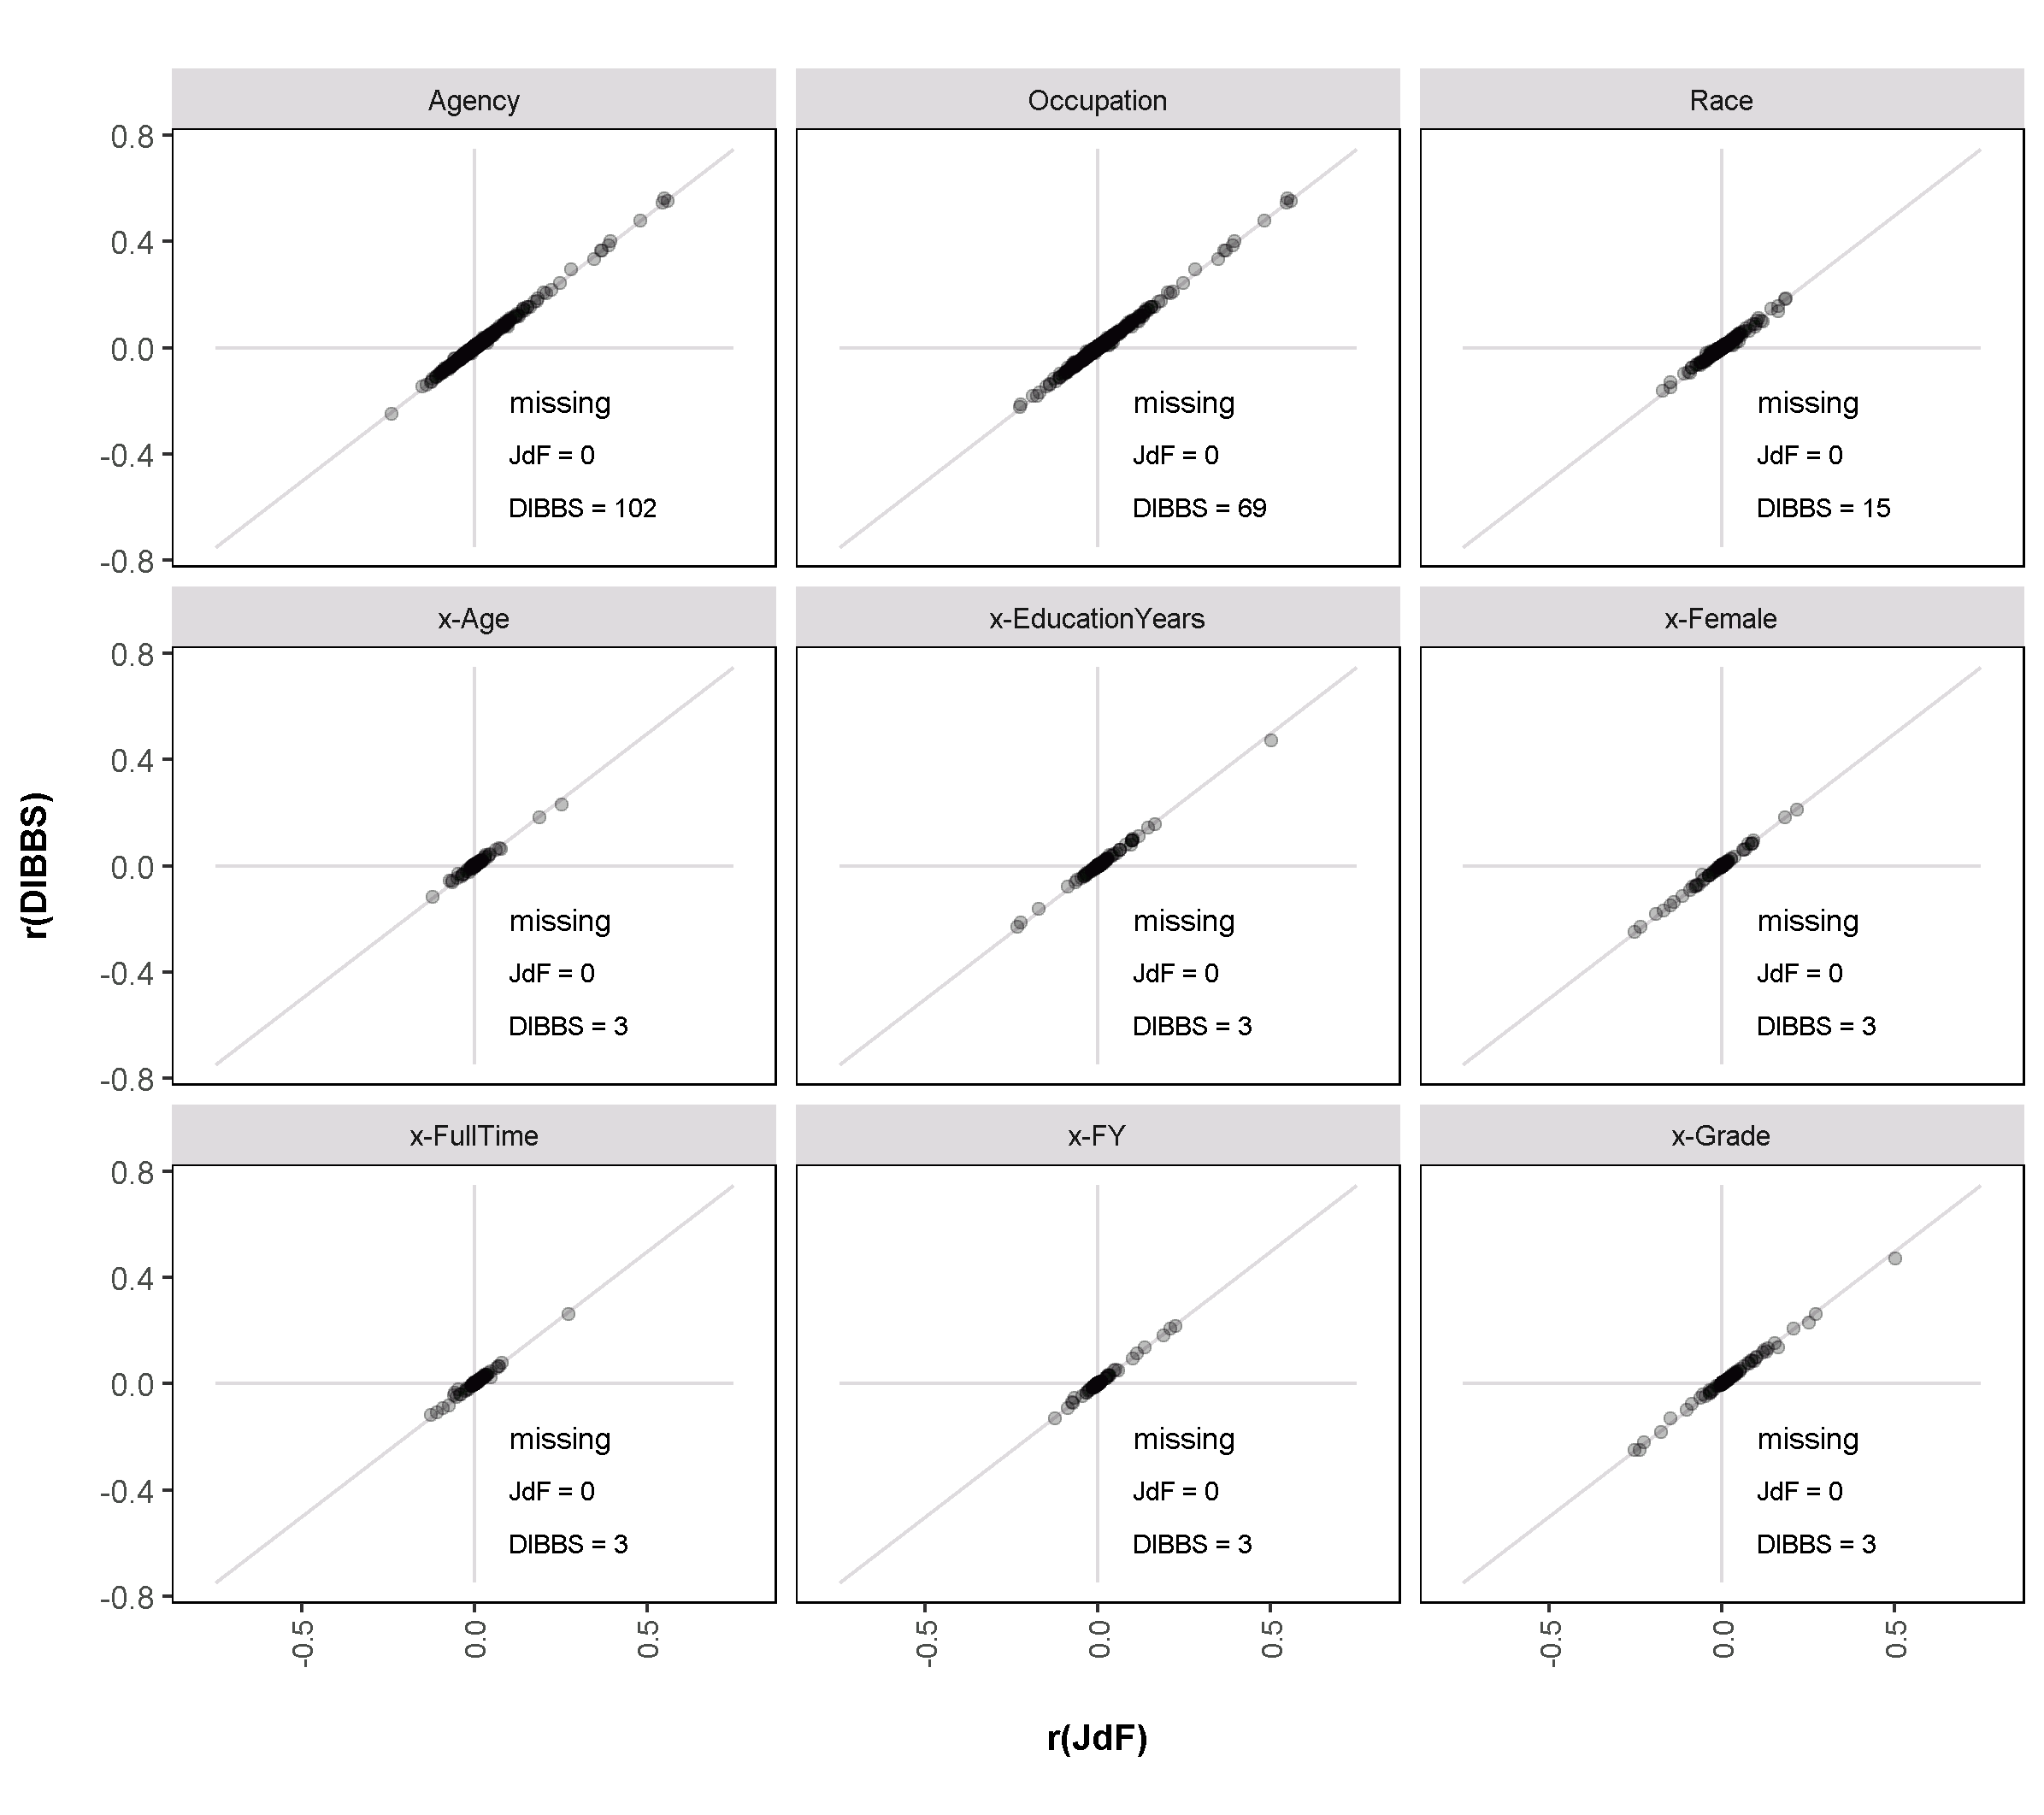
\includegraphics[width=6.5in]{JdFDIBBSCorrelation.png}
    \centering
    \caption{Two variable correlations of corresponding levels of synthetic and authentic data.  Synthetic level correlation on y-axis, corresponding authentic correlation on x-axis.}
    \label{figure:JdFDIBBSCorrelation}
\end{figure}  

\clearpage

CORRELATION OF PRIMARY VARIABLES WITH TWO-VARIABLE INTERACTIONS\\

Figures \ref{figure:JdFDIBBSCorrelationInteraction} and \ref{figure:JdFDIBBSCorrelationInteraction2} show, for pay plan GS, full-time observations, correlations between 1.) the variable indicated in the graph title, 2.) all combinations of levels of the variable listed in a title bar, and 3.) all levels of other variables appearing in the title bars.  These constitute correlation of main variables with two variable interactions.  In the case of categorical variables, or fixed effects, this is the association of a primary variable with the proportion of observations in interacting level combinations of two other variables.  Agency and occupation truncated to first two positions.\\

Observation:  Proximity of all points to slope 1.0 reference line indicates agreement of three-variable associations between data sets and implies depth of utility beyond simple pairwise relationships.\\

\begin{figure}[ht]
    \centering
    \begin{subfigure}{.5\textwidth}
        \centering
        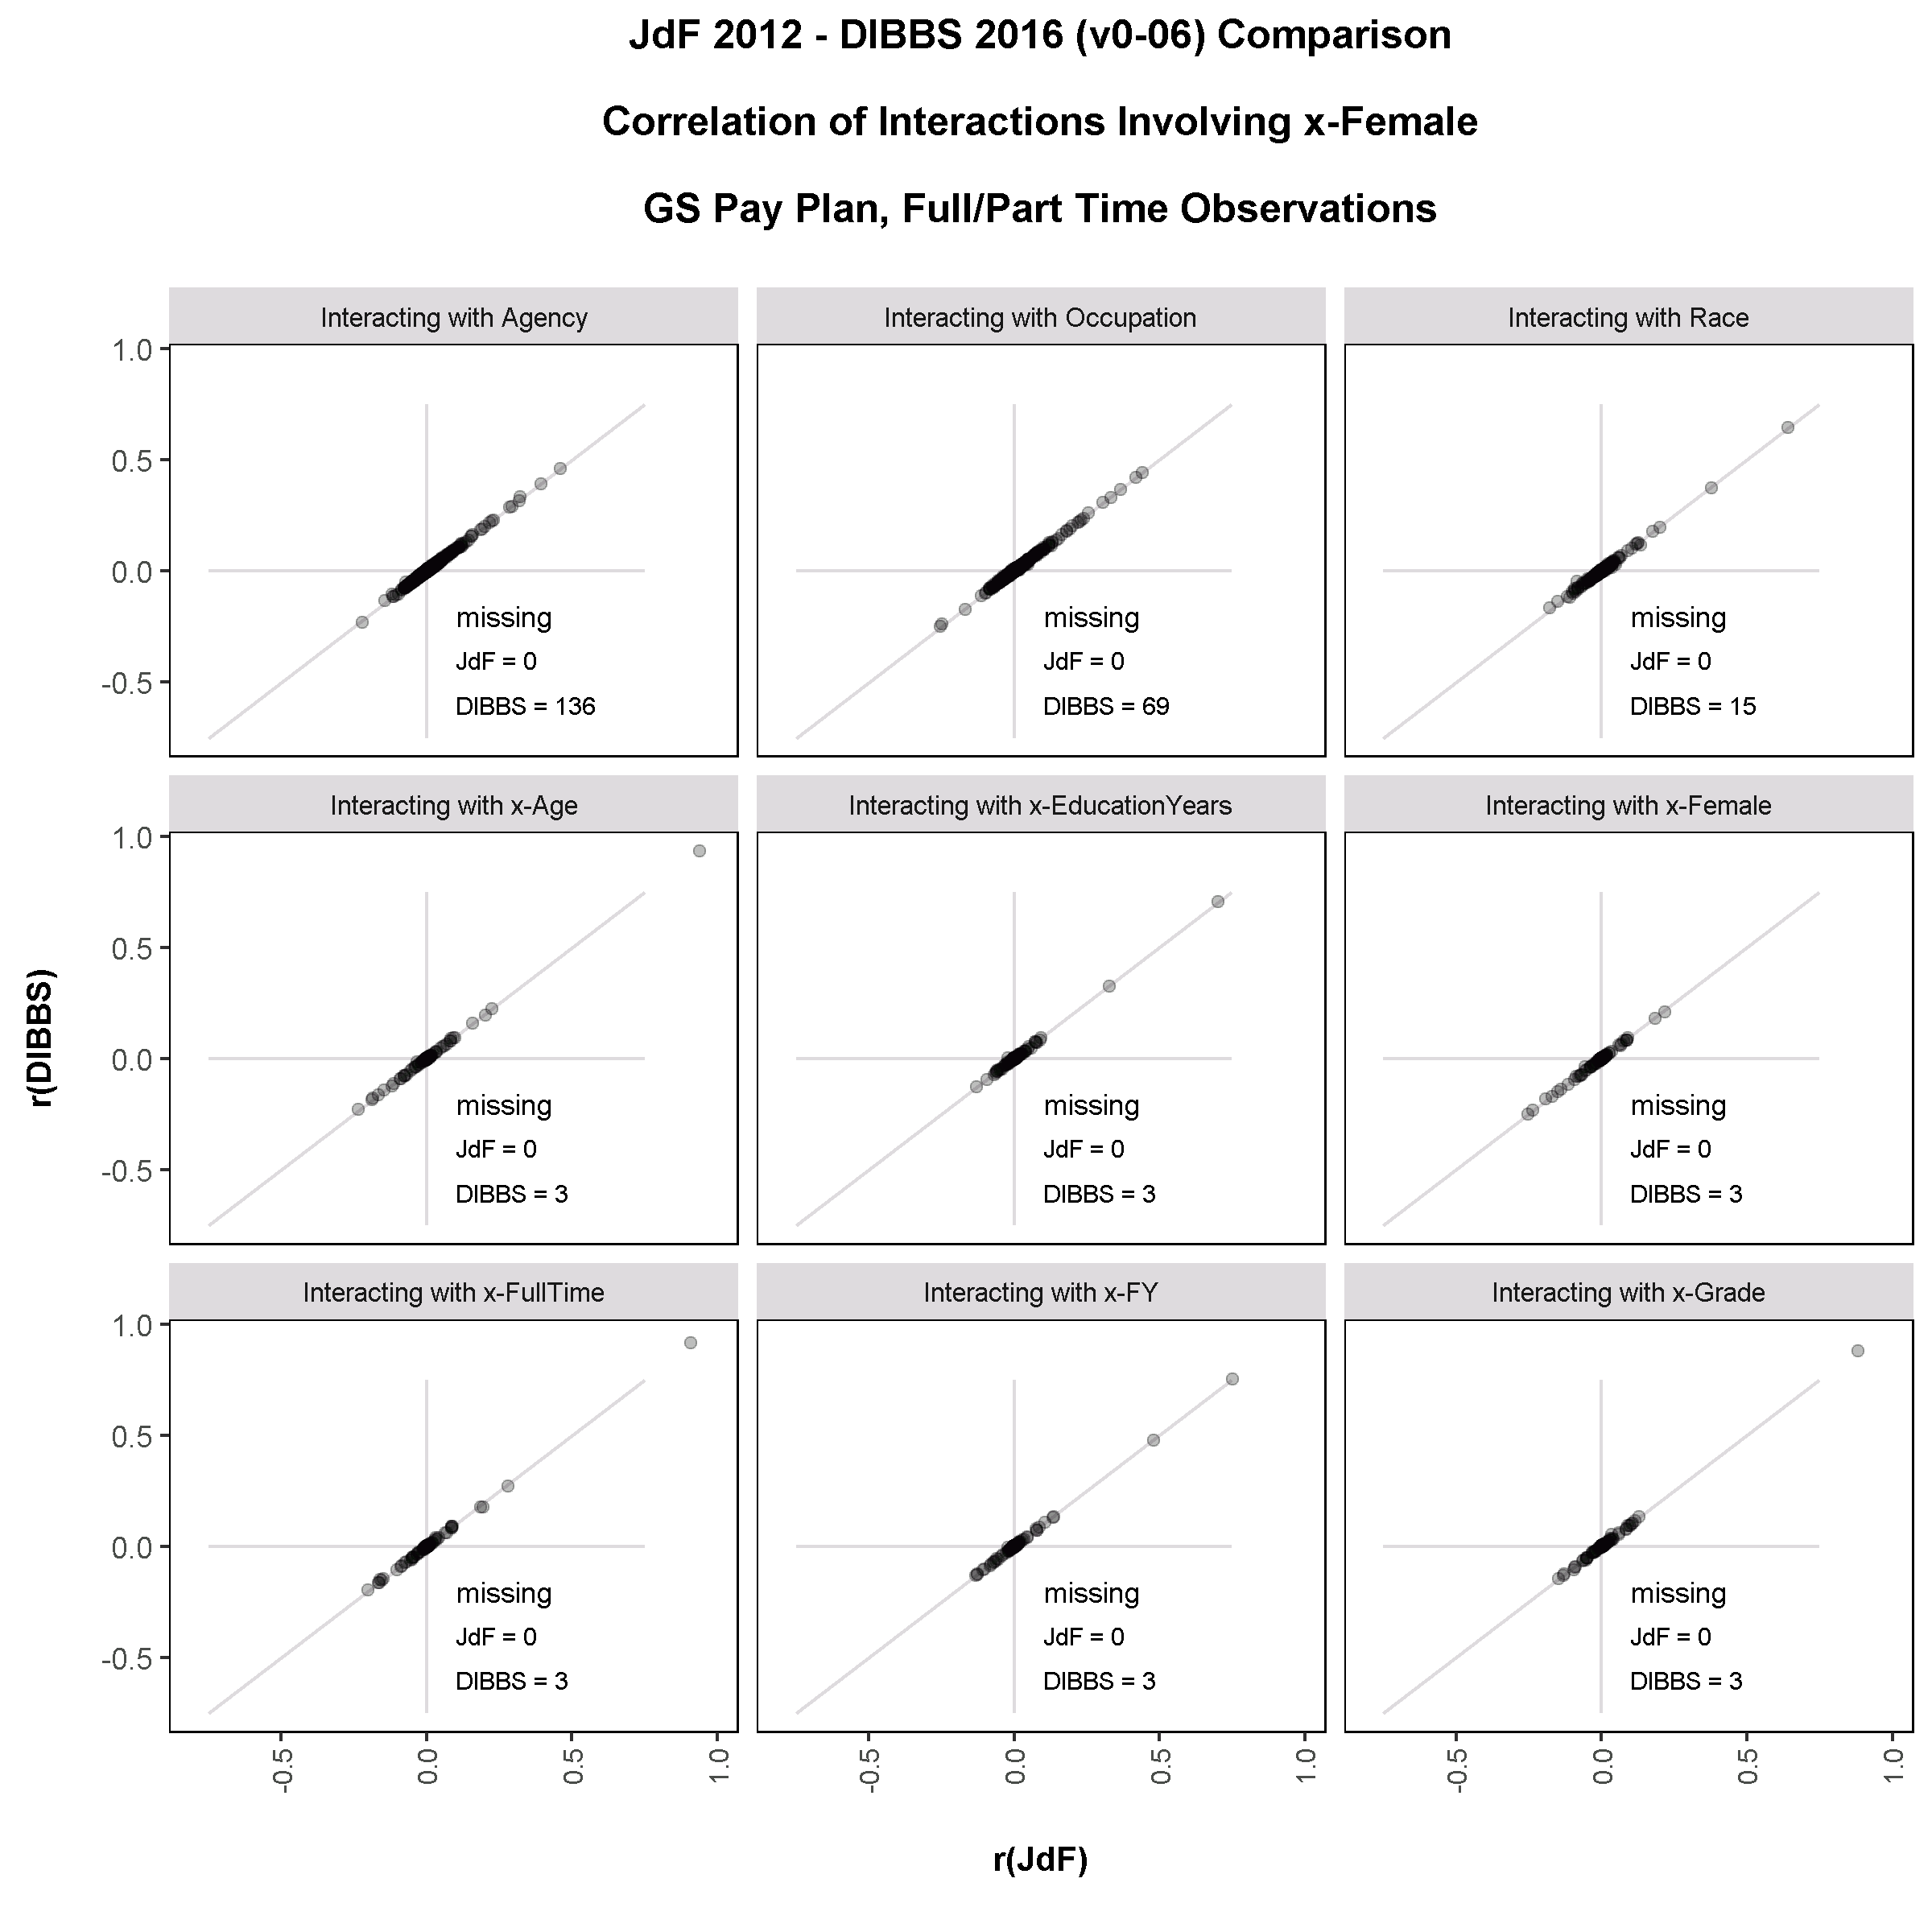
\includegraphics[width=3in, trim={0 0.25in 0 1in}, clip]{JdFDIBBSCorrelationInteraction-x-Female.png}
        \caption{Correlations involving sex}
        %\label{figure:}
        \vspace{10pt}
    \end{subfigure}% suppress line break
    \begin{subfigure}{.5\textwidth}
        \centering
        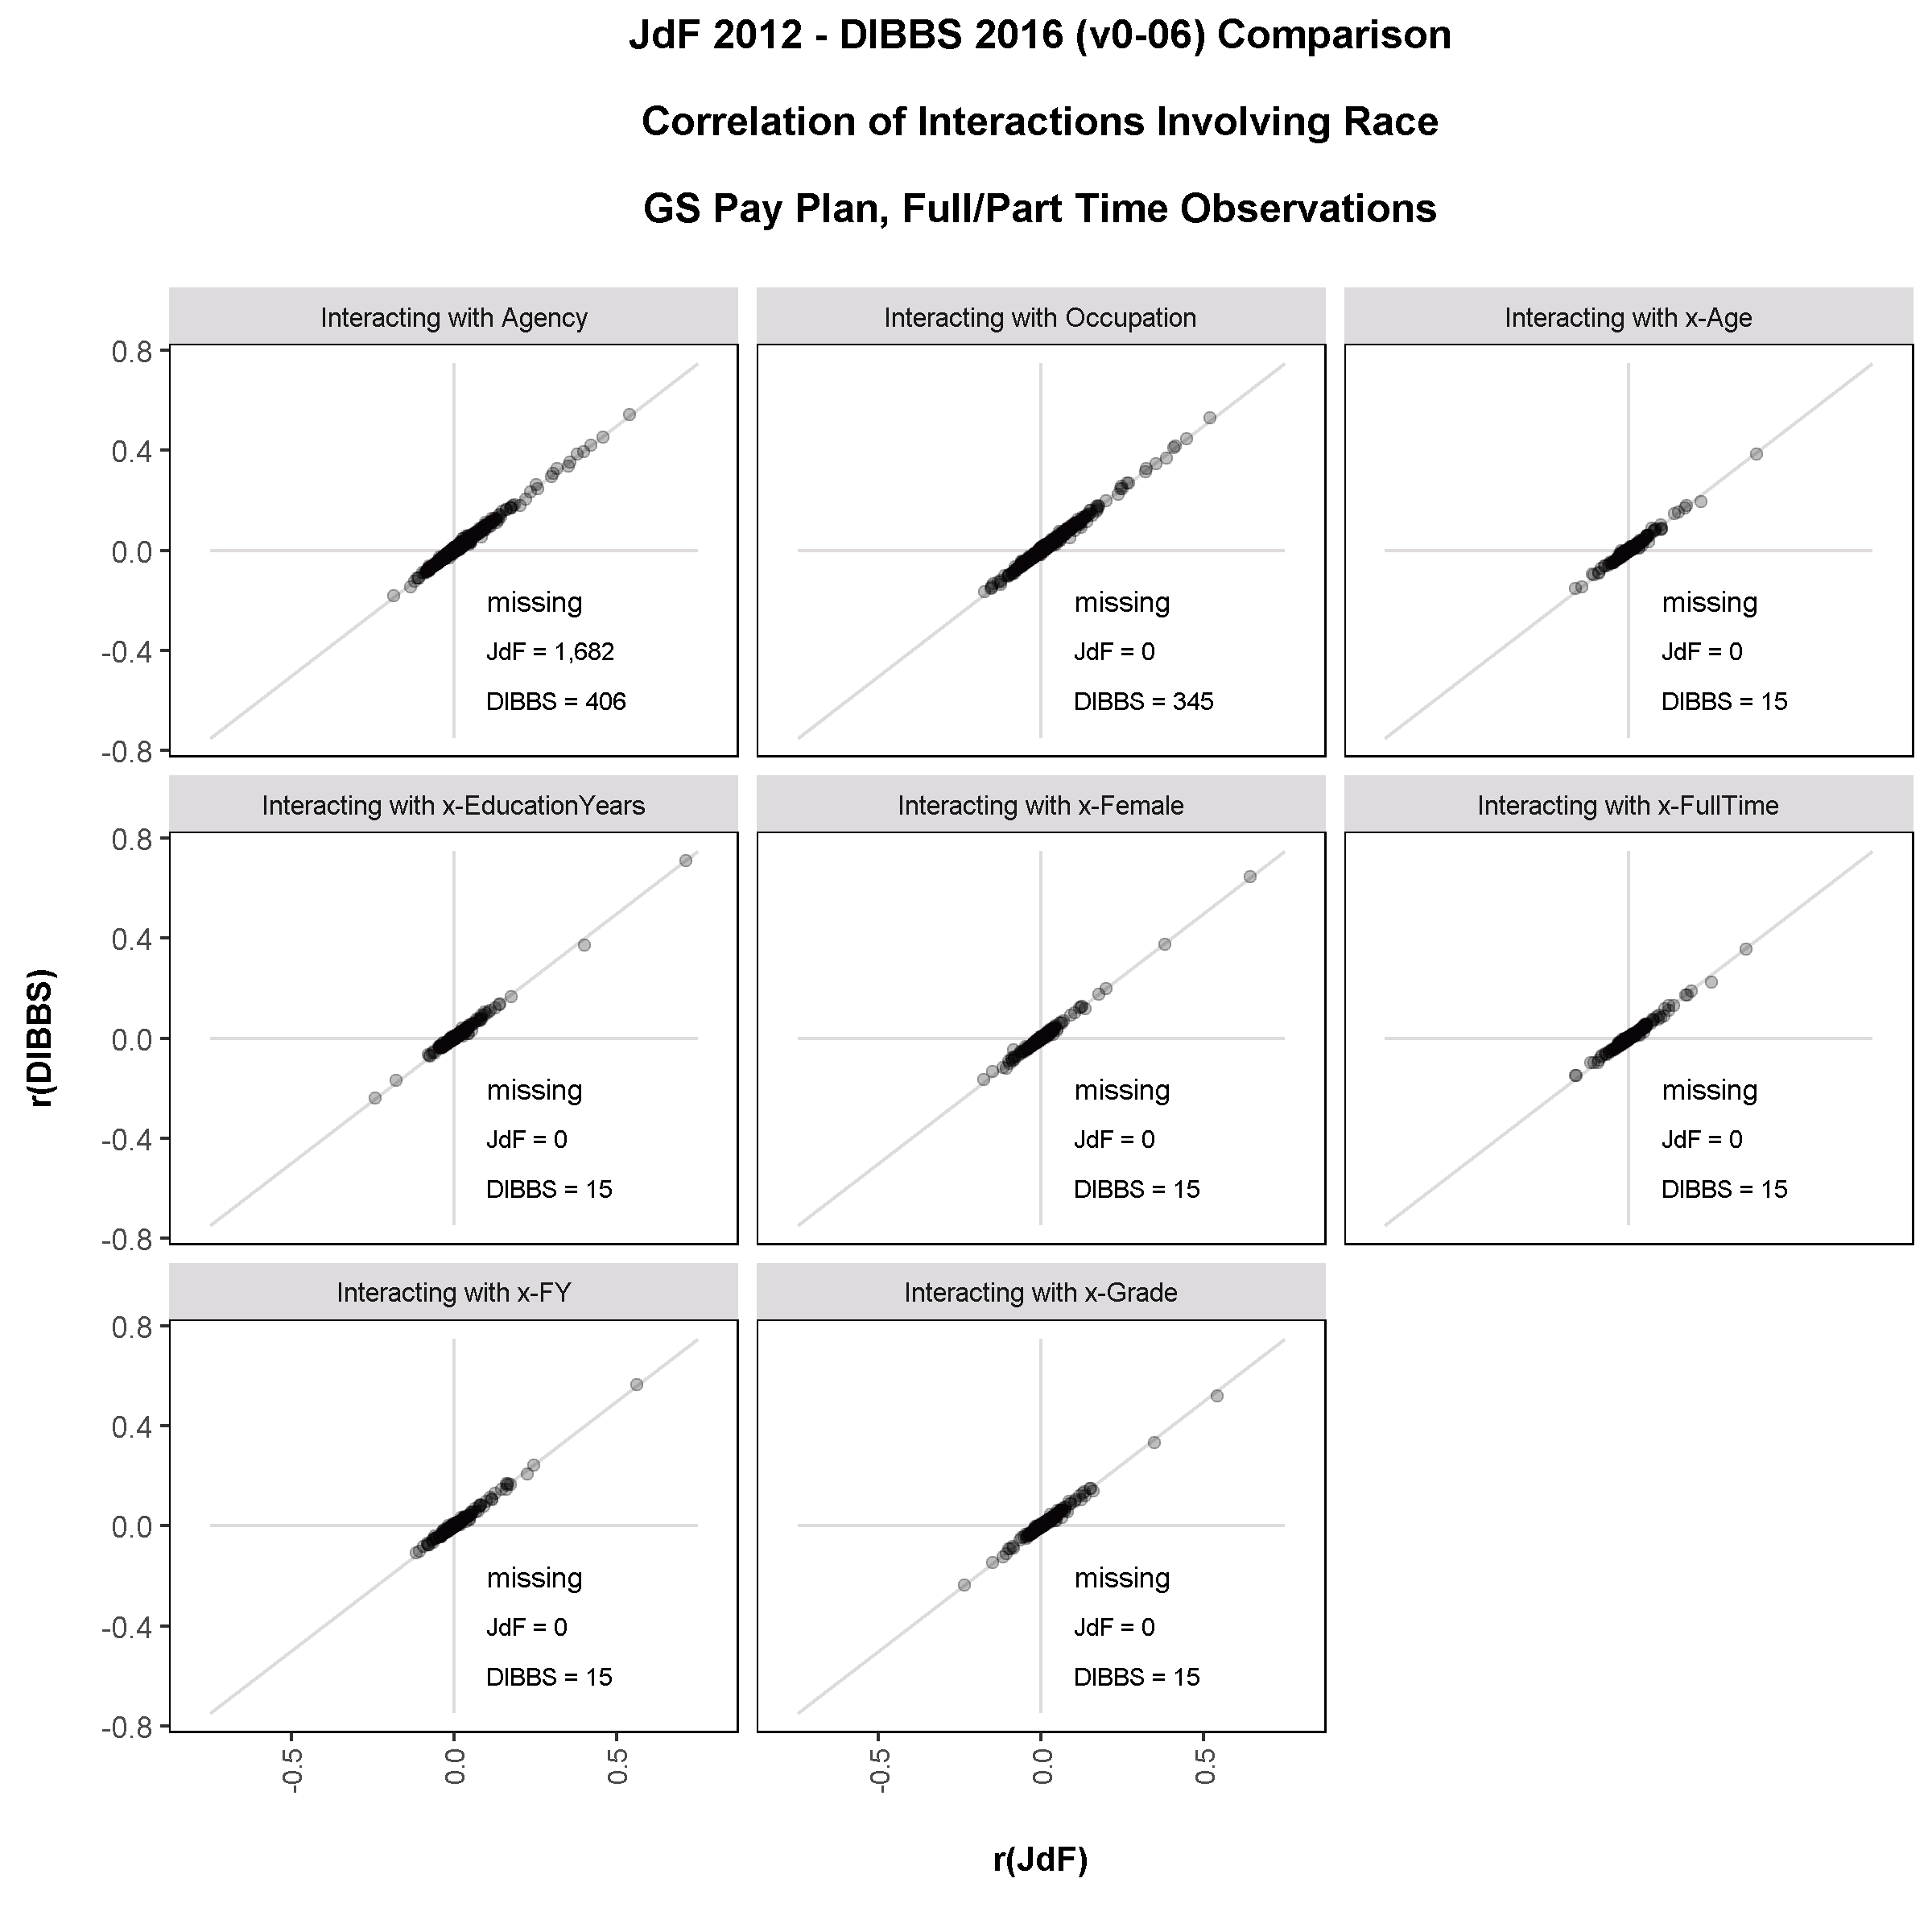
\includegraphics[width=3in, trim={0 0.25in 0 1in}, clip]{JdFDIBBSCorrelationInteraction-Race.png}
        \caption{Correlations involving race}
        %\label{figure:}
        \vspace{10pt}
    \end{subfigure}
    \begin{subfigure}{.5\textwidth}
        \centering
        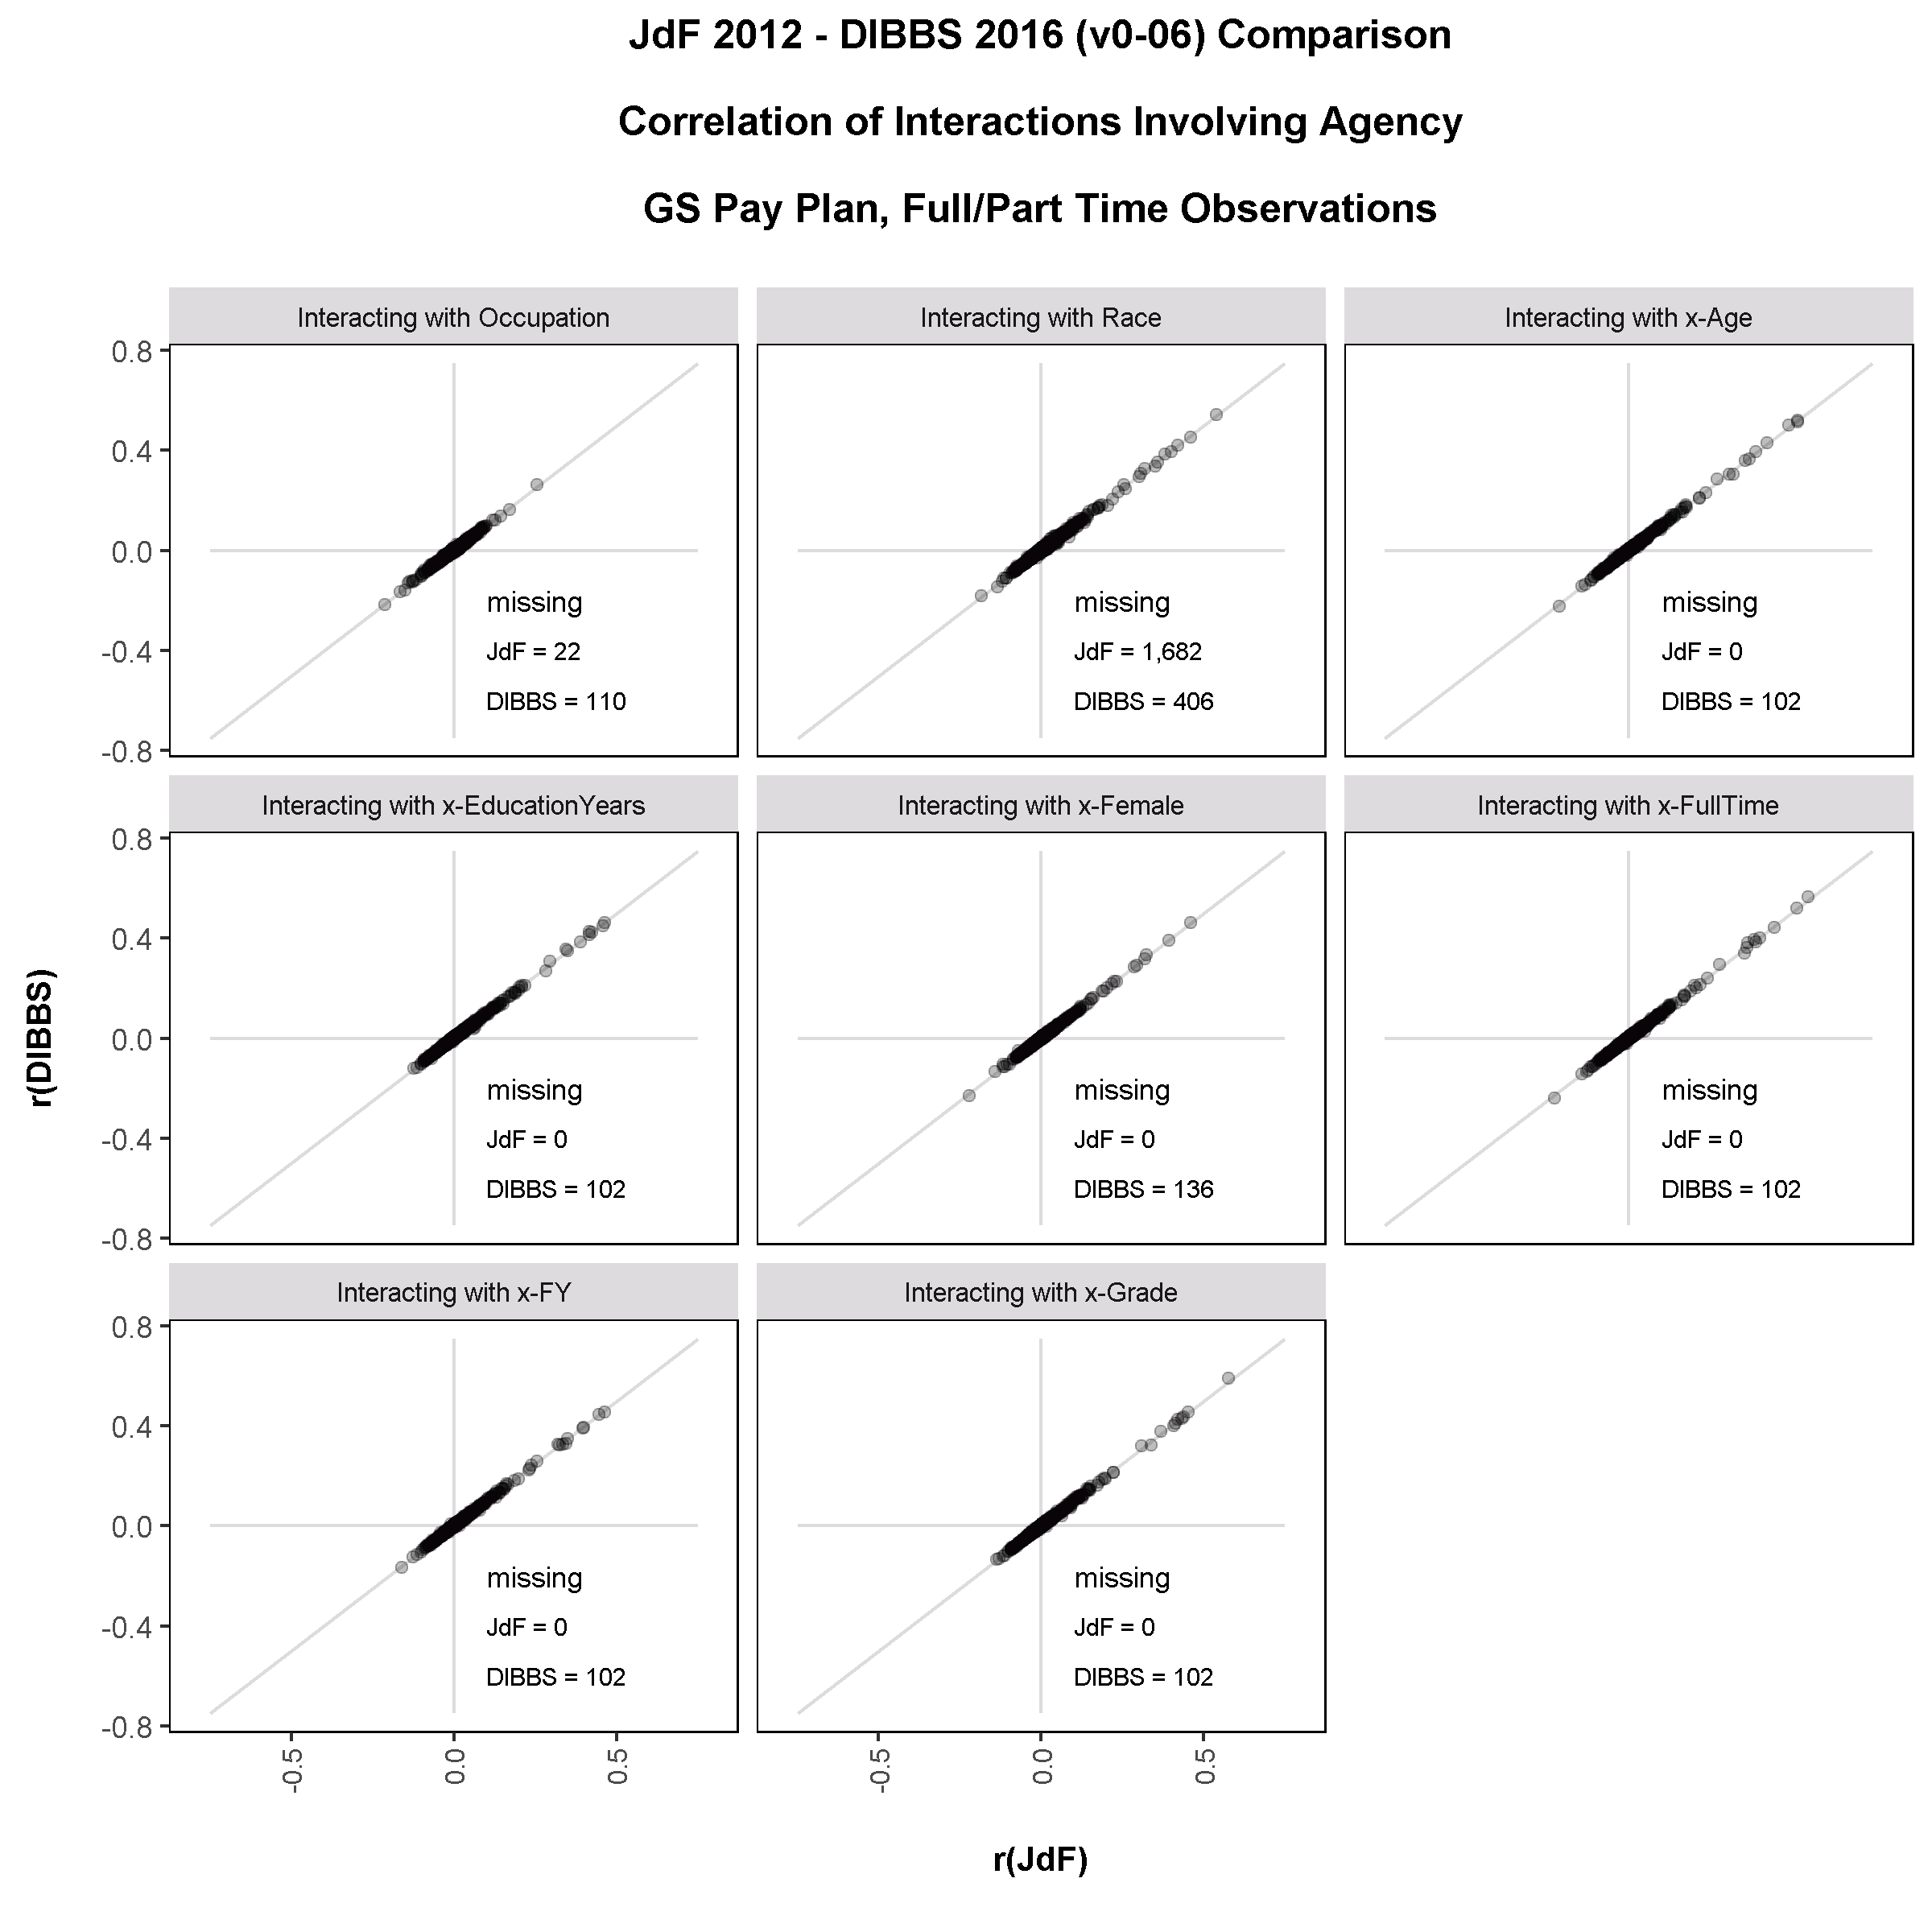
\includegraphics[width=3in, trim={0 0.25in 0 1in}, clip]{JdFDIBBSCorrelationInteraction-Agency.png}
        \caption{Correlations involving agency}
        %\label{figure:}
        \vspace{10pt}
    \end{subfigure}% suppress line break
    \begin{subfigure}{.5\textwidth}
        \centering
        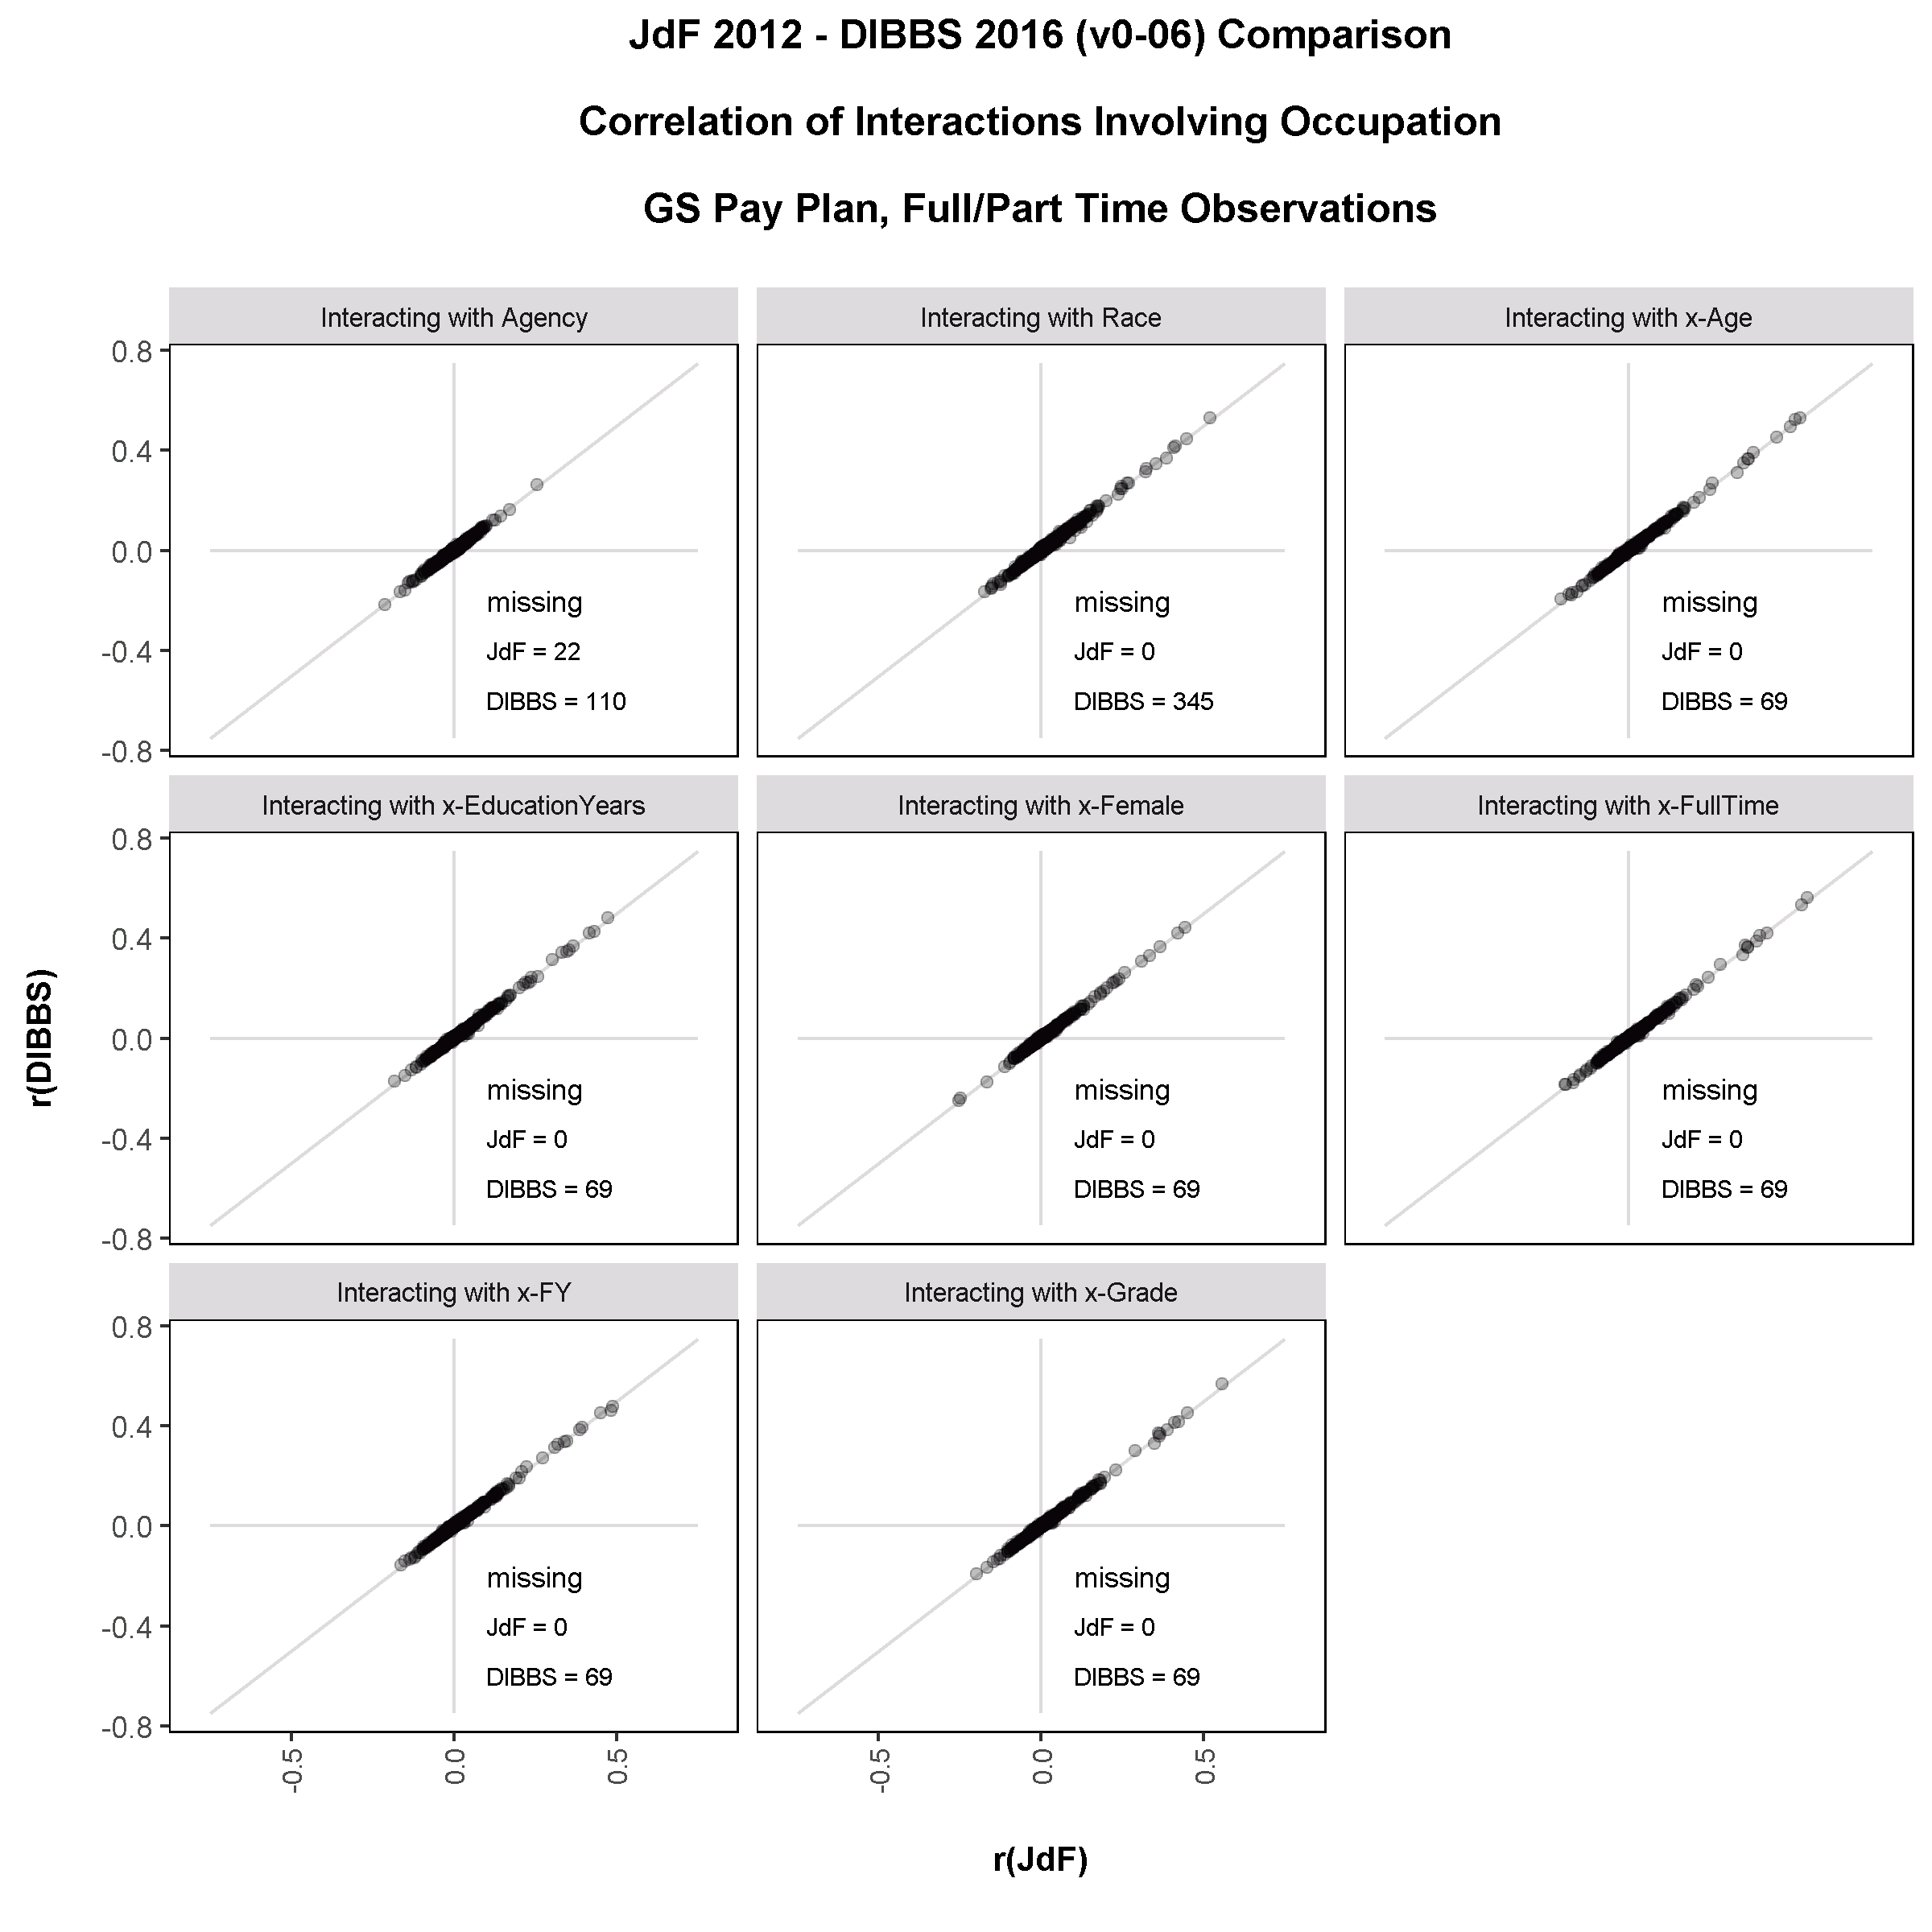
\includegraphics[width=3in, trim={0 0.25in 0 1in}, clip]{JdFDIBBSCorrelationInteraction-Occupation.png}
        \caption{Correlations involving occupation}
        %\label{figure:}
        \vspace{10pt}
    \end{subfigure}
    \caption{Correlations of primary variables with two variable interactions.  Variable set one.  Synthetic level correlation on y-axis, corresponding authentic correlation on x-axis.}
    \label{figure:JdFDIBBSCorrelationInteraction}
\end{figure}

\begin{figure}[ht]
    \centering
    \begin{subfigure}{.5\textwidth}
        \centering
        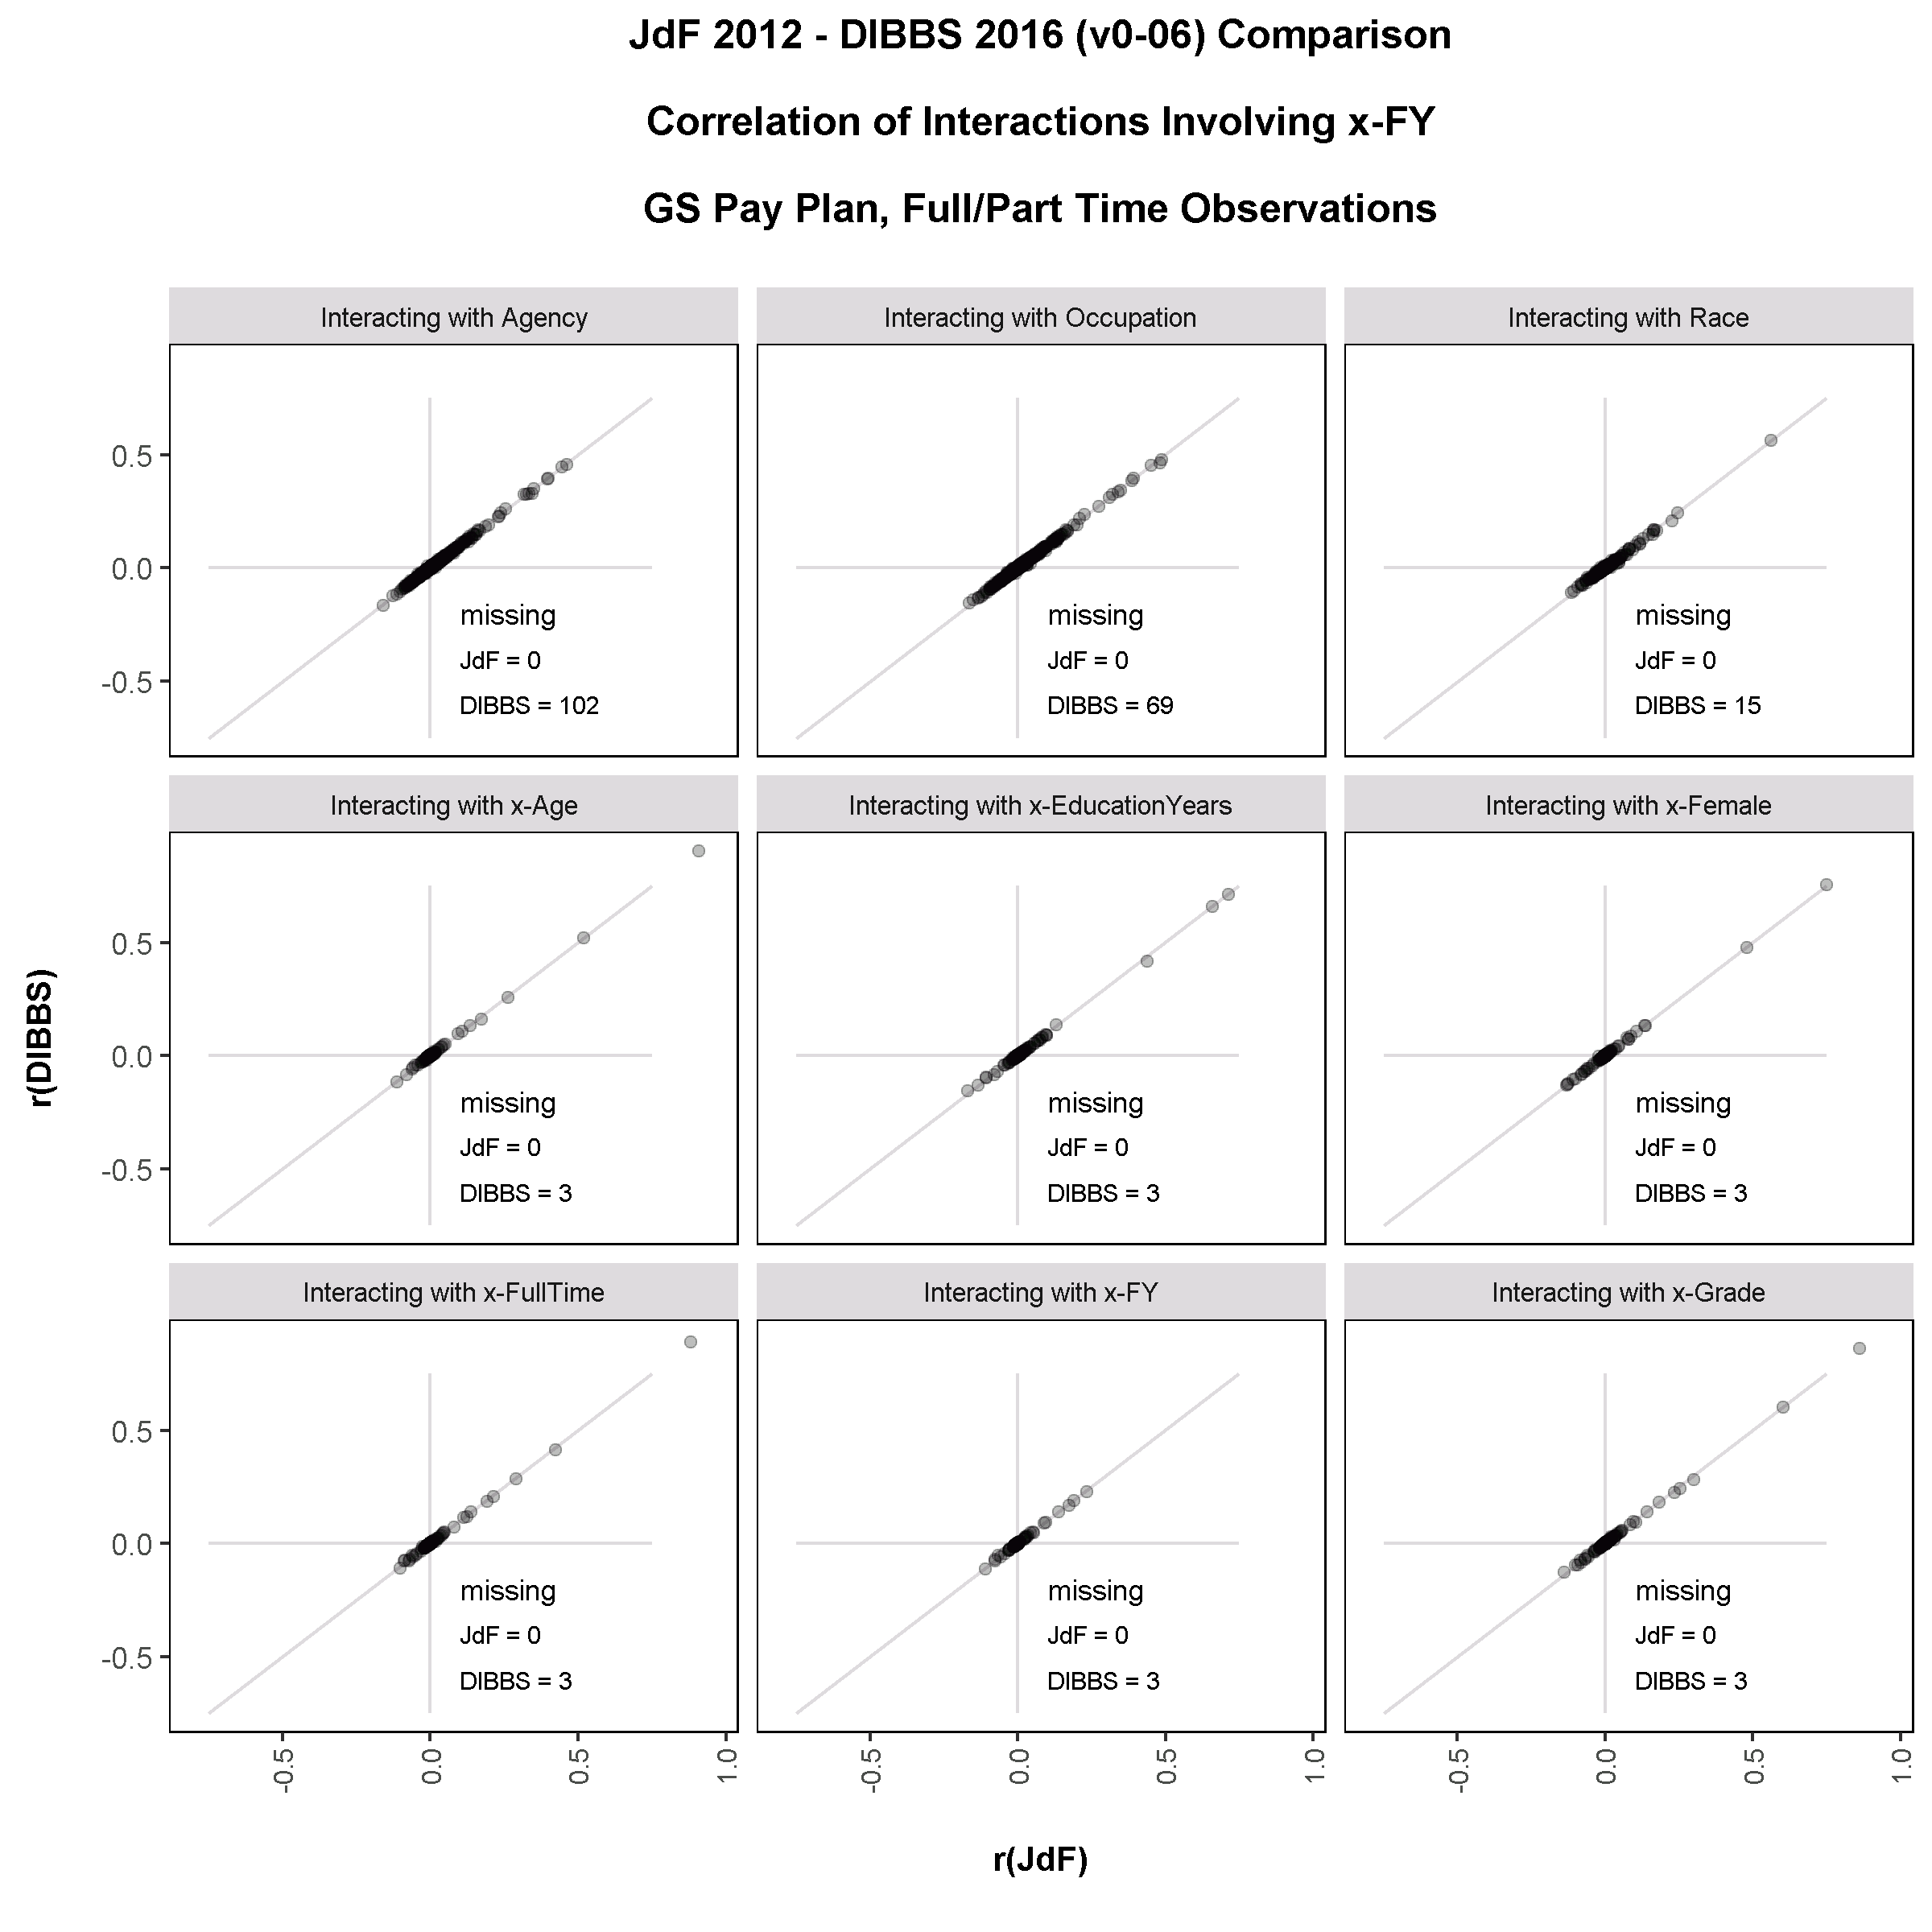
\includegraphics[width=3in, trim={0 0.25in 0 1in}, clip]{JdFDIBBSCorrelationInteraction-x-FY.png}
        \caption{Correlations involving Fiscal Year}
        %\label{figure:}
        \vspace{10pt}
    \end{subfigure}% suppress line break
    \begin{subfigure}{.5\textwidth}
        \centering
        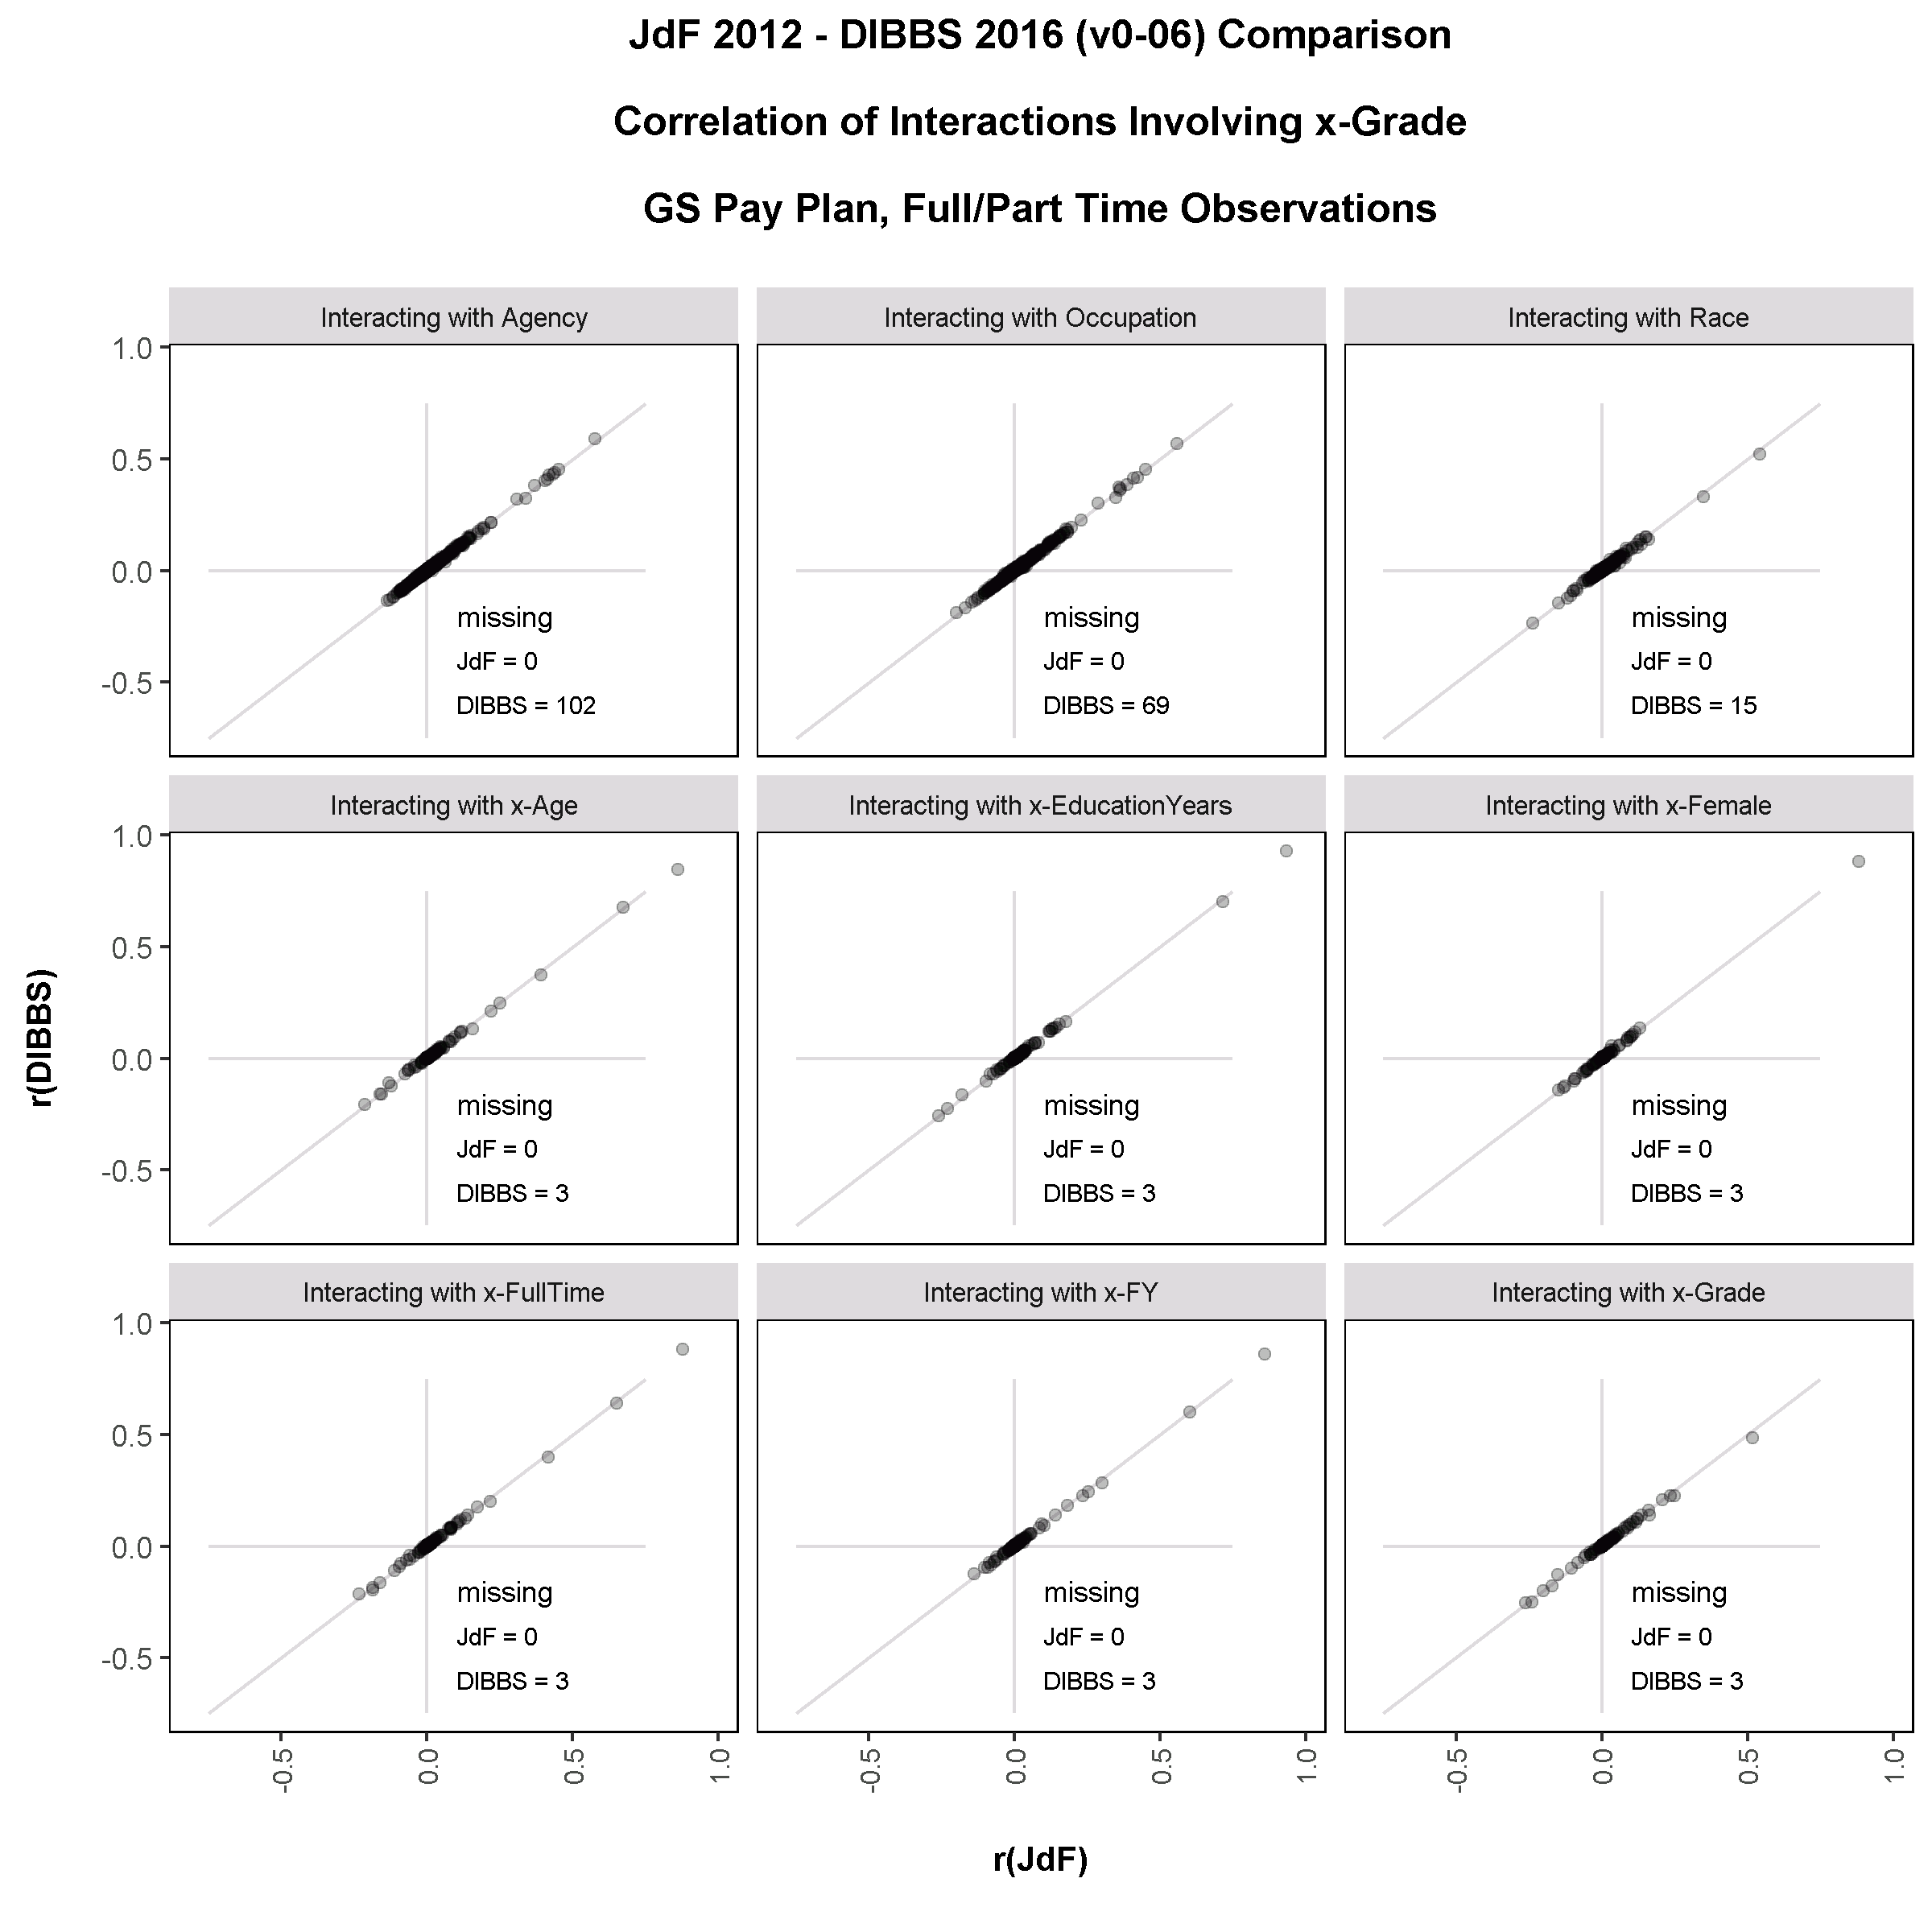
\includegraphics[width=3in, trim={0 0.25in 0 1in}, clip]{JdFDIBBSCorrelationInteraction-x-Grade.png}
        \caption{Correlations involving Grade}
        %\label{figure:}
        \vspace{10pt}
    \end{subfigure}
    \begin{subfigure}{.5\textwidth}
        \centering
        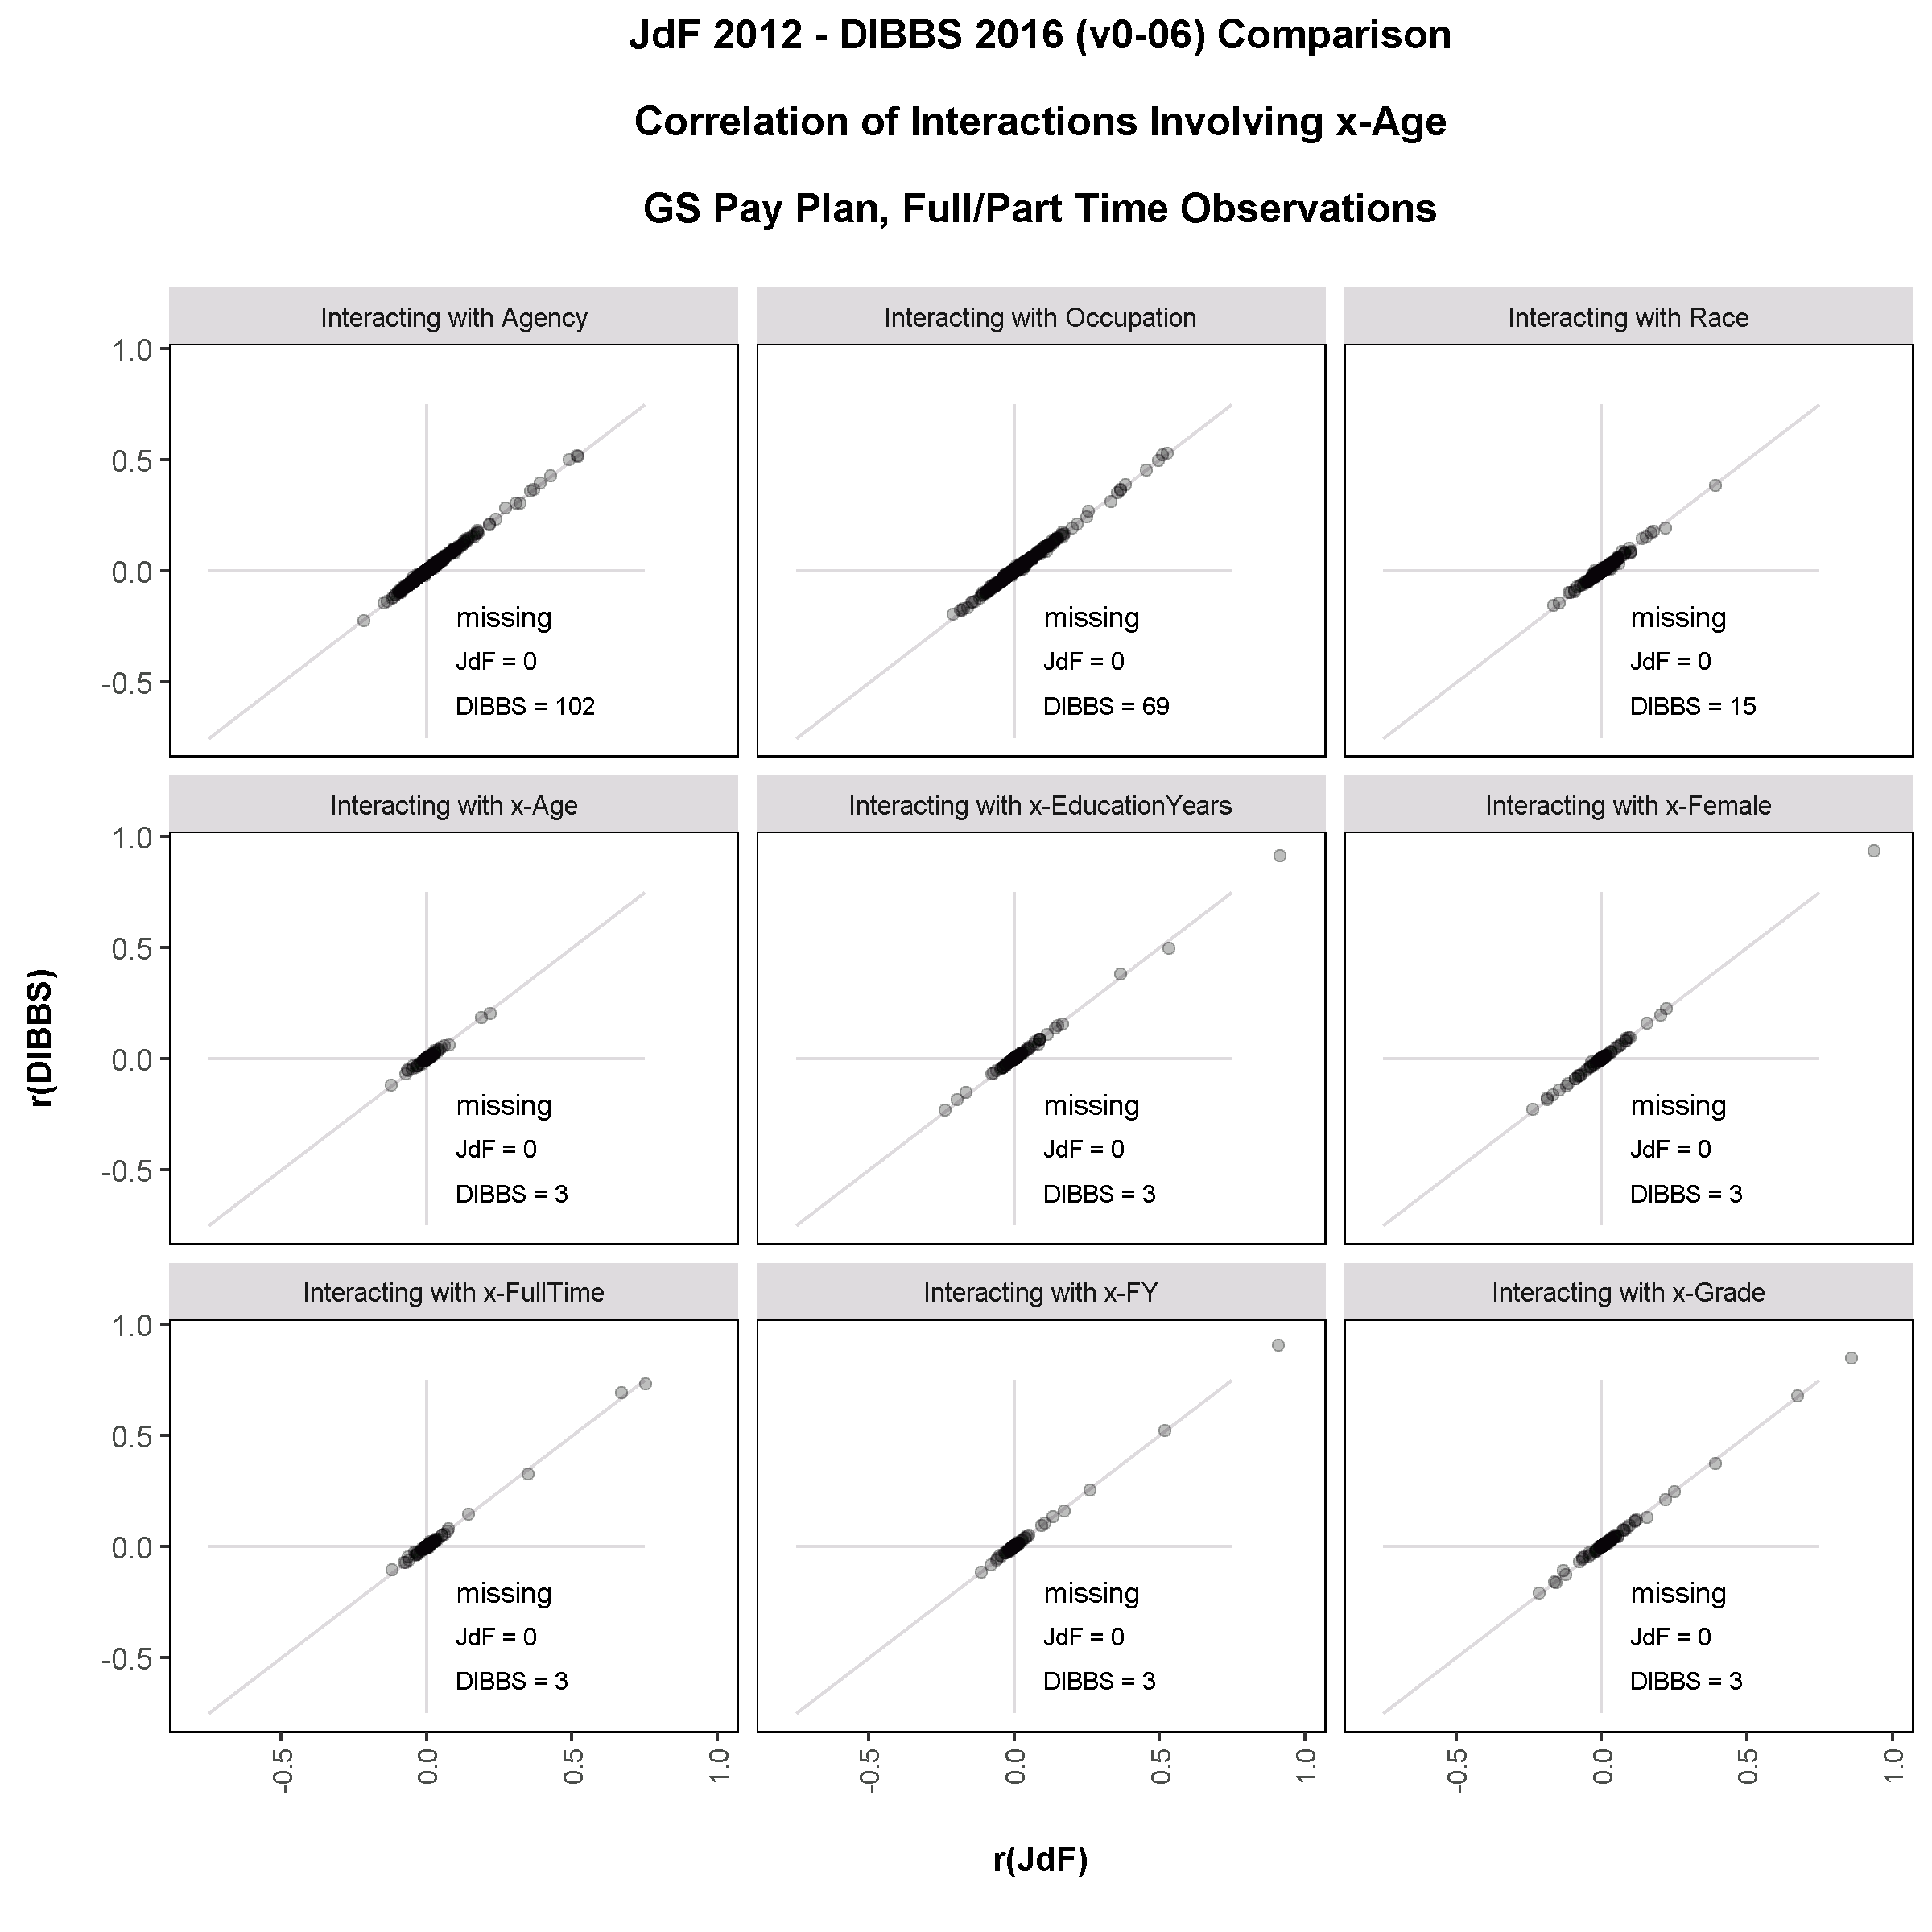
\includegraphics[width=3in, trim={0 0.25in 0 1in}, clip]{JdFDIBBSCorrelationInteraction-x-Age.png}
        \caption{Correlations involving Age}
        %\label{figure:}
        \vspace{10pt}
    \end{subfigure}% suppress line break
    \begin{subfigure}{.5\textwidth}
        \centering
        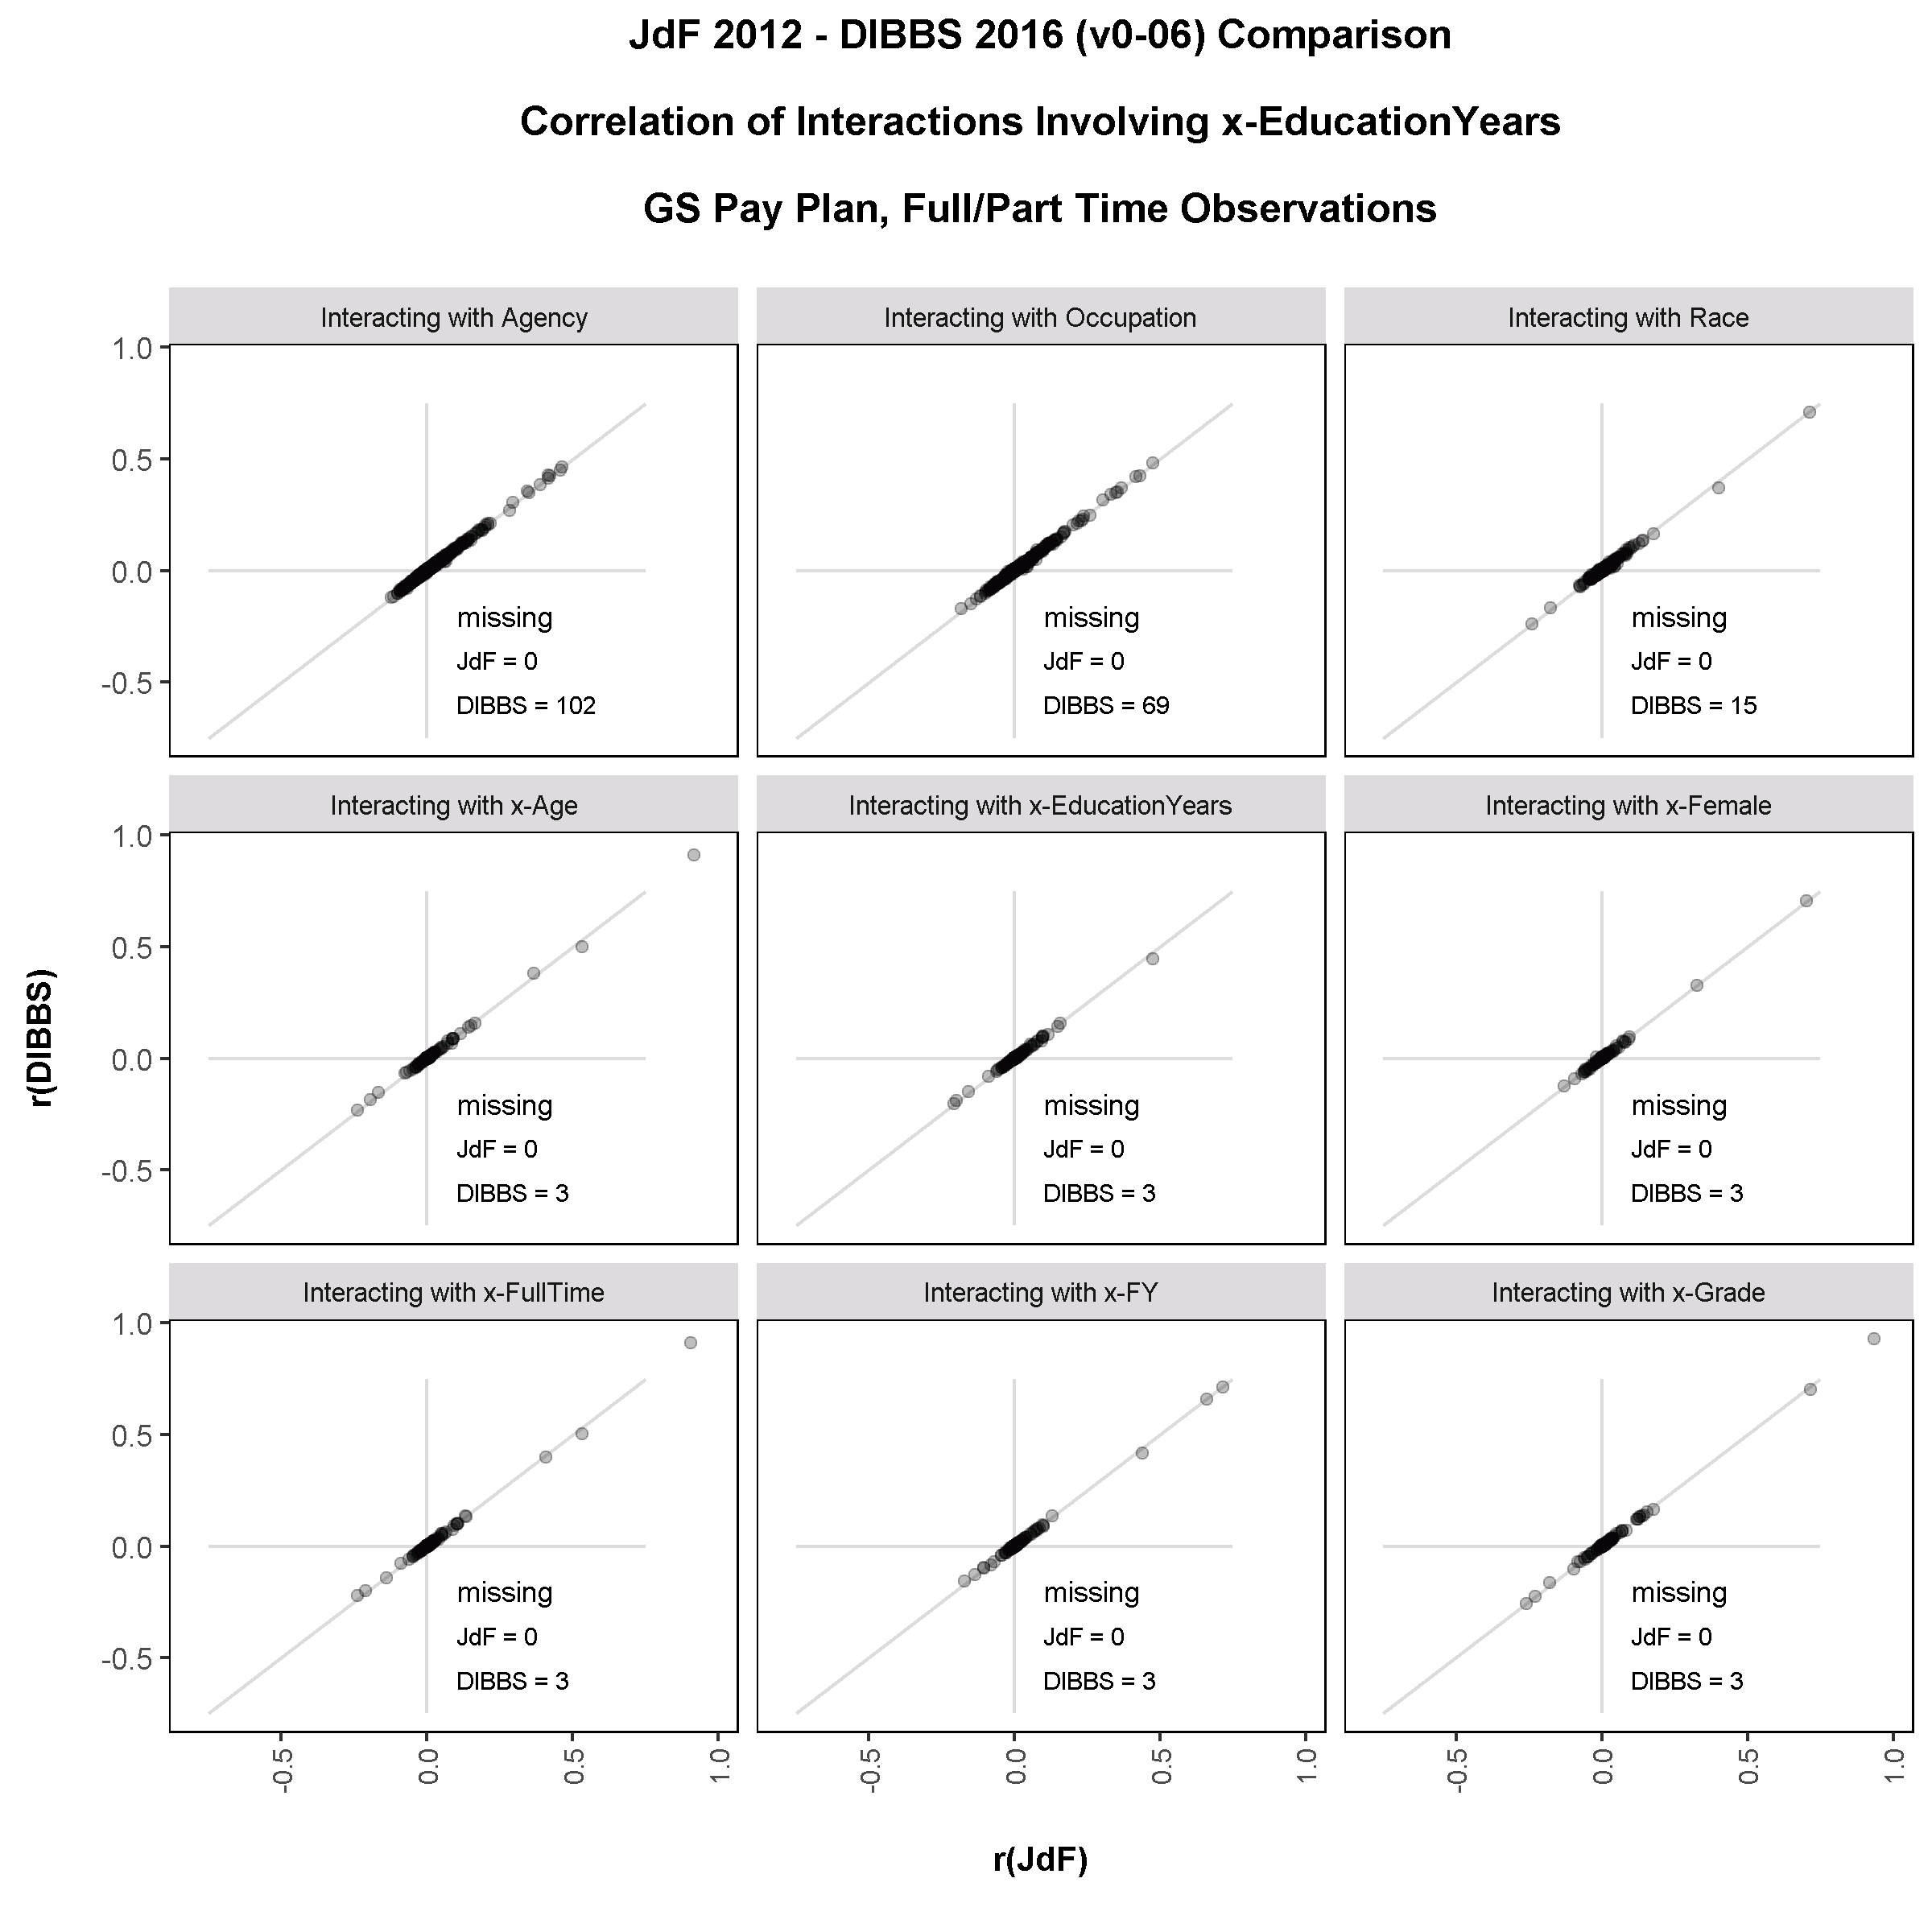
\includegraphics[width=3in, trim={0 0.25in 0 1in}, clip]{JdFDIBBSCorrelationInteraction-x-EducationYears.png}
        \caption{Correlations involving Education}
        %\label{figure:}
        \vspace{10pt}
    \end{subfigure}
    \begin{subfigure}{.5\textwidth}
        \centering
        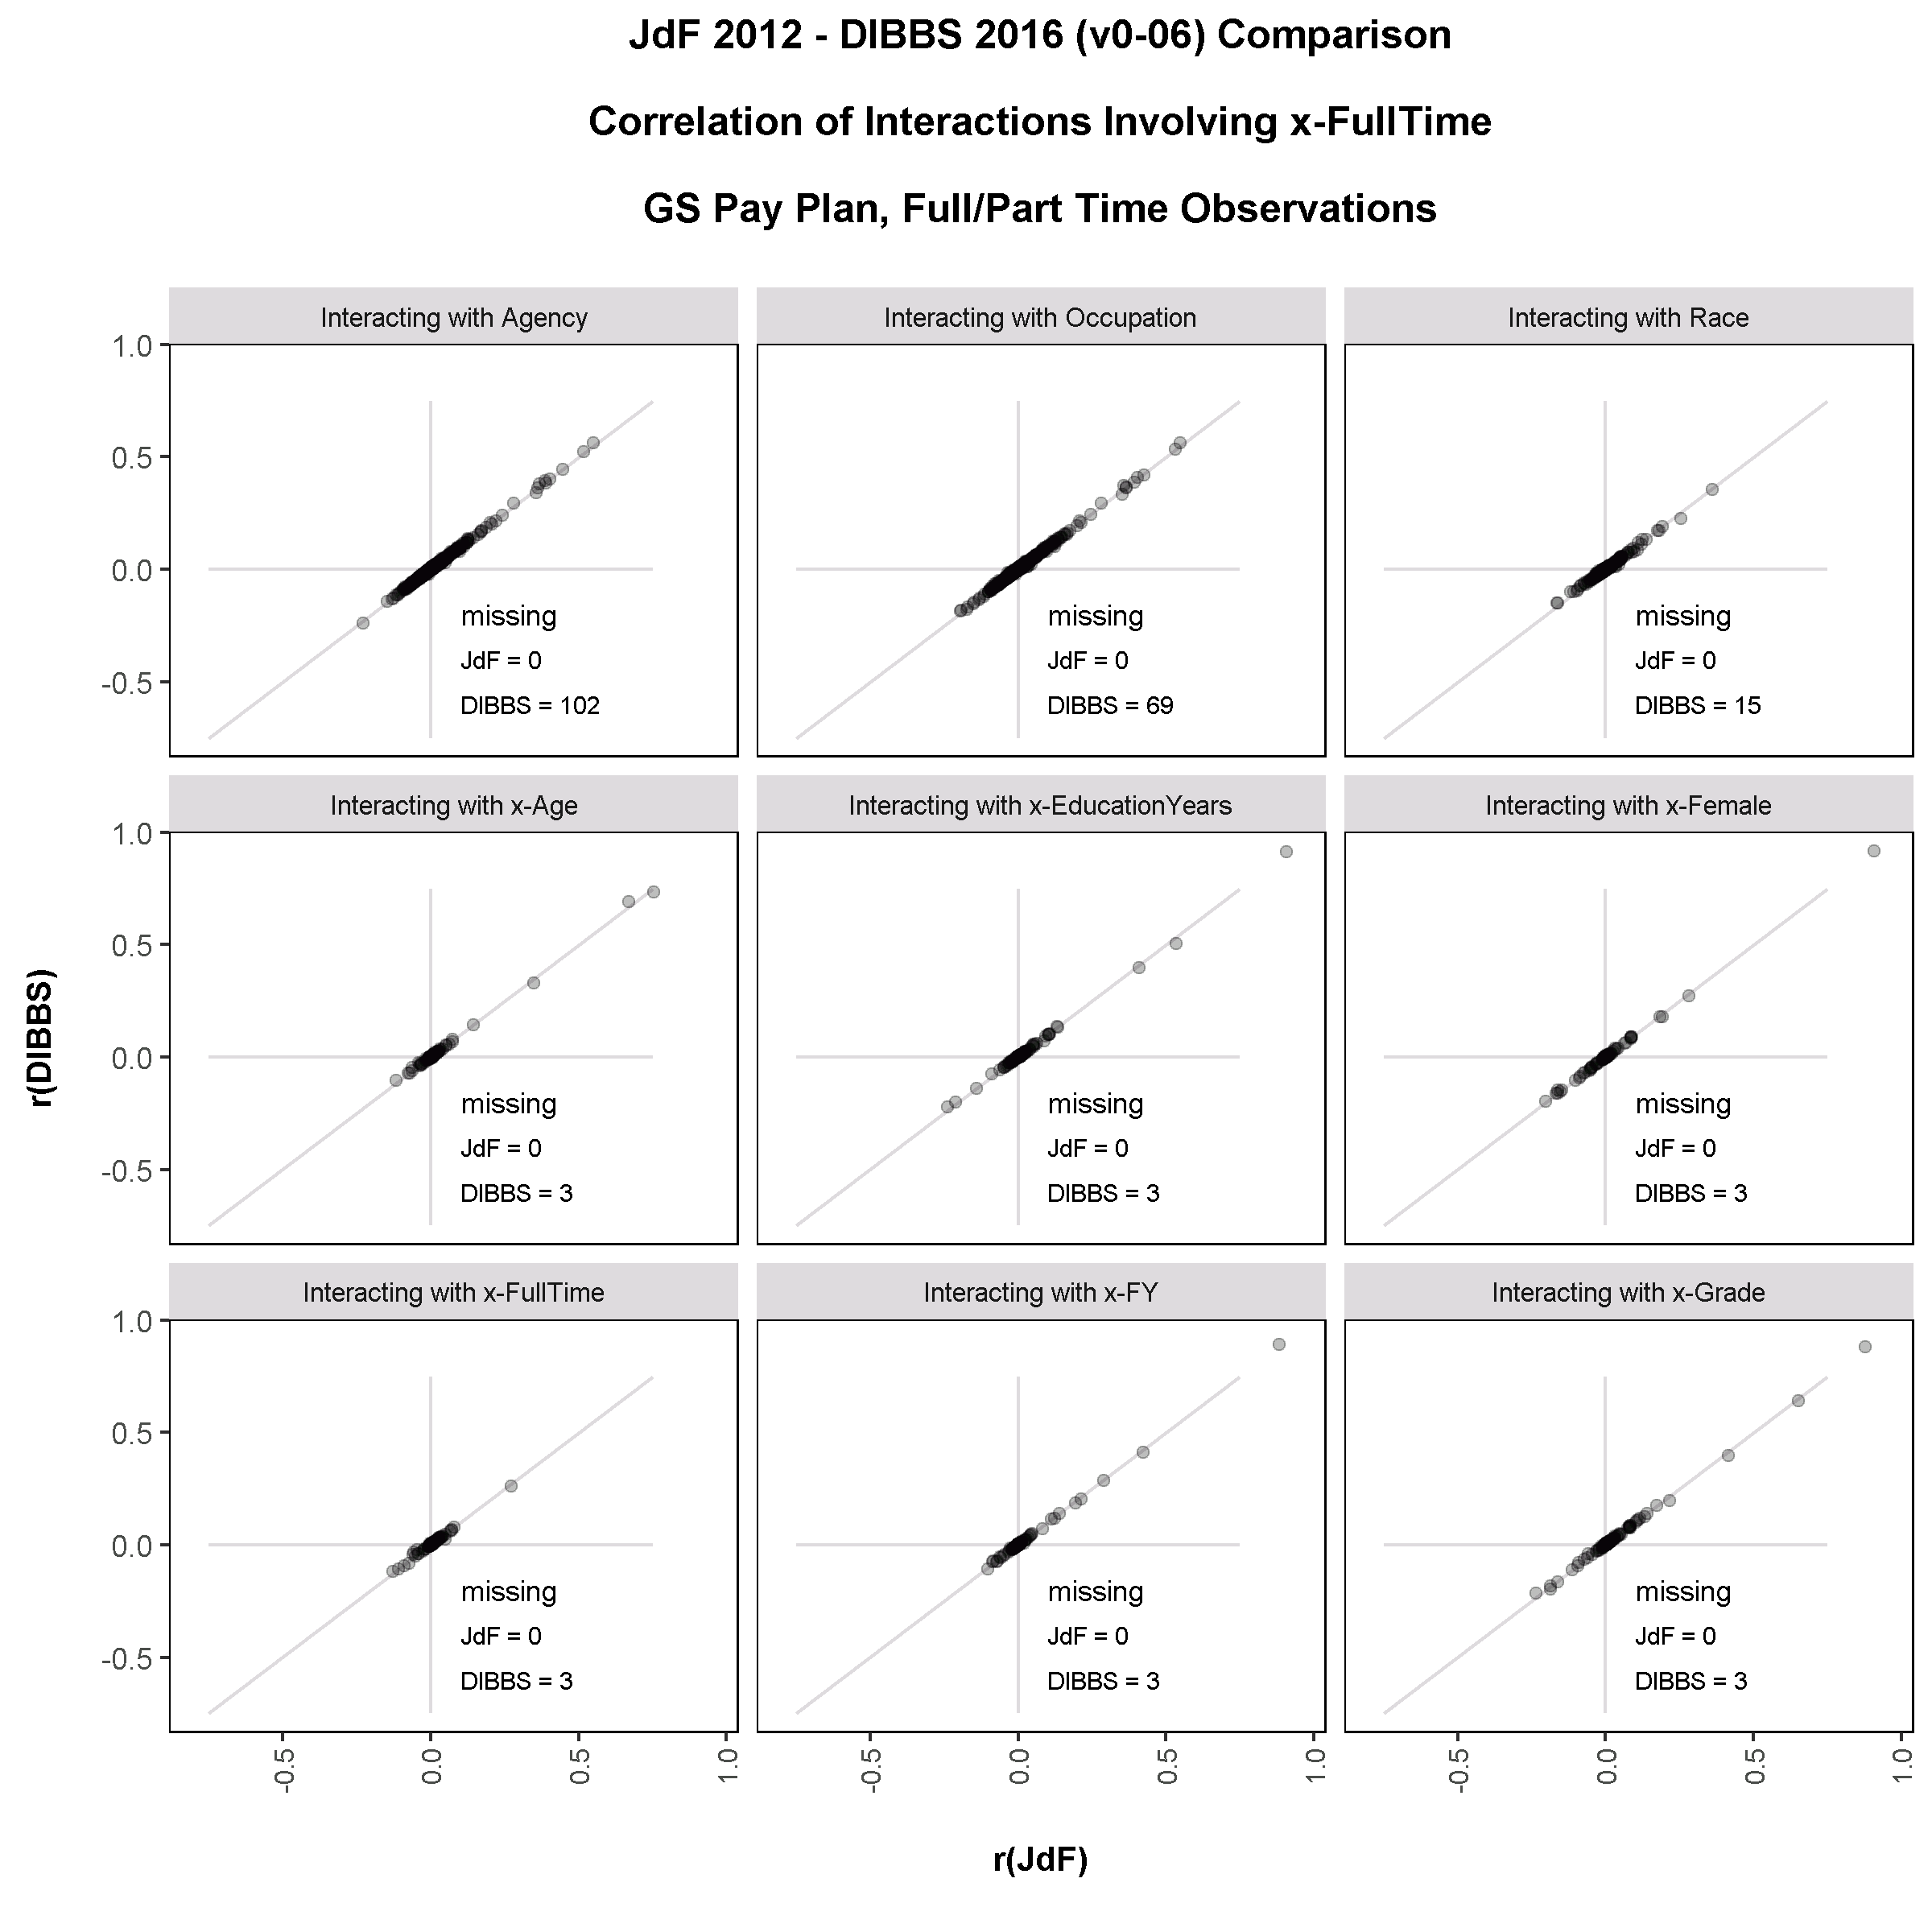
\includegraphics[width=3in, trim={0 0.25in 0 1in}, clip]{JdFDIBBSCorrelationInteraction-x-FullTime.png}
        \caption{Correlations involving Work Schedule}
        %\label{figure:}
        \vspace{10pt}
    \end{subfigure}
    \caption{Correlations of primary variables with two variable interactions.  Variable set two.  Synthetic level correlation on y-axis, corresponding authentic correlation on x-axis.}
    \label{figure:JdFDIBBSCorrelationInteraction2}
\end{figure}  

\clearpage

CUMULATIVE MASS (PROPORTION OBSERVATIONS) BY PAY PLAN AND OCCUPATION\\

Figures \ref{figure:CMFOccupationPayPlan1} and \ref{figure:CMFOccupationPayPlan2} contain example CMF plots of pay plan and occupation combinations.  All occupations within each pay plan are represented.  Solid line for authentic data, dashed line for synthetic.  Overlapping or nearness of lines indicates equality of cumulative mass for corresponding levels of occupation within pay plan.  ``nJ" indicates observation count in authentic data, ``nD" indicates synthetic data observation count.  Near identical distribution is observed for high frequency pay plans GS, WG, GM, and VN, which account for more than 95\% of observations, indicating overall close agreement between data sets.  Increasing departure observed as number of observations decreases.\\

\begin{figure}[h!]
    \centering
    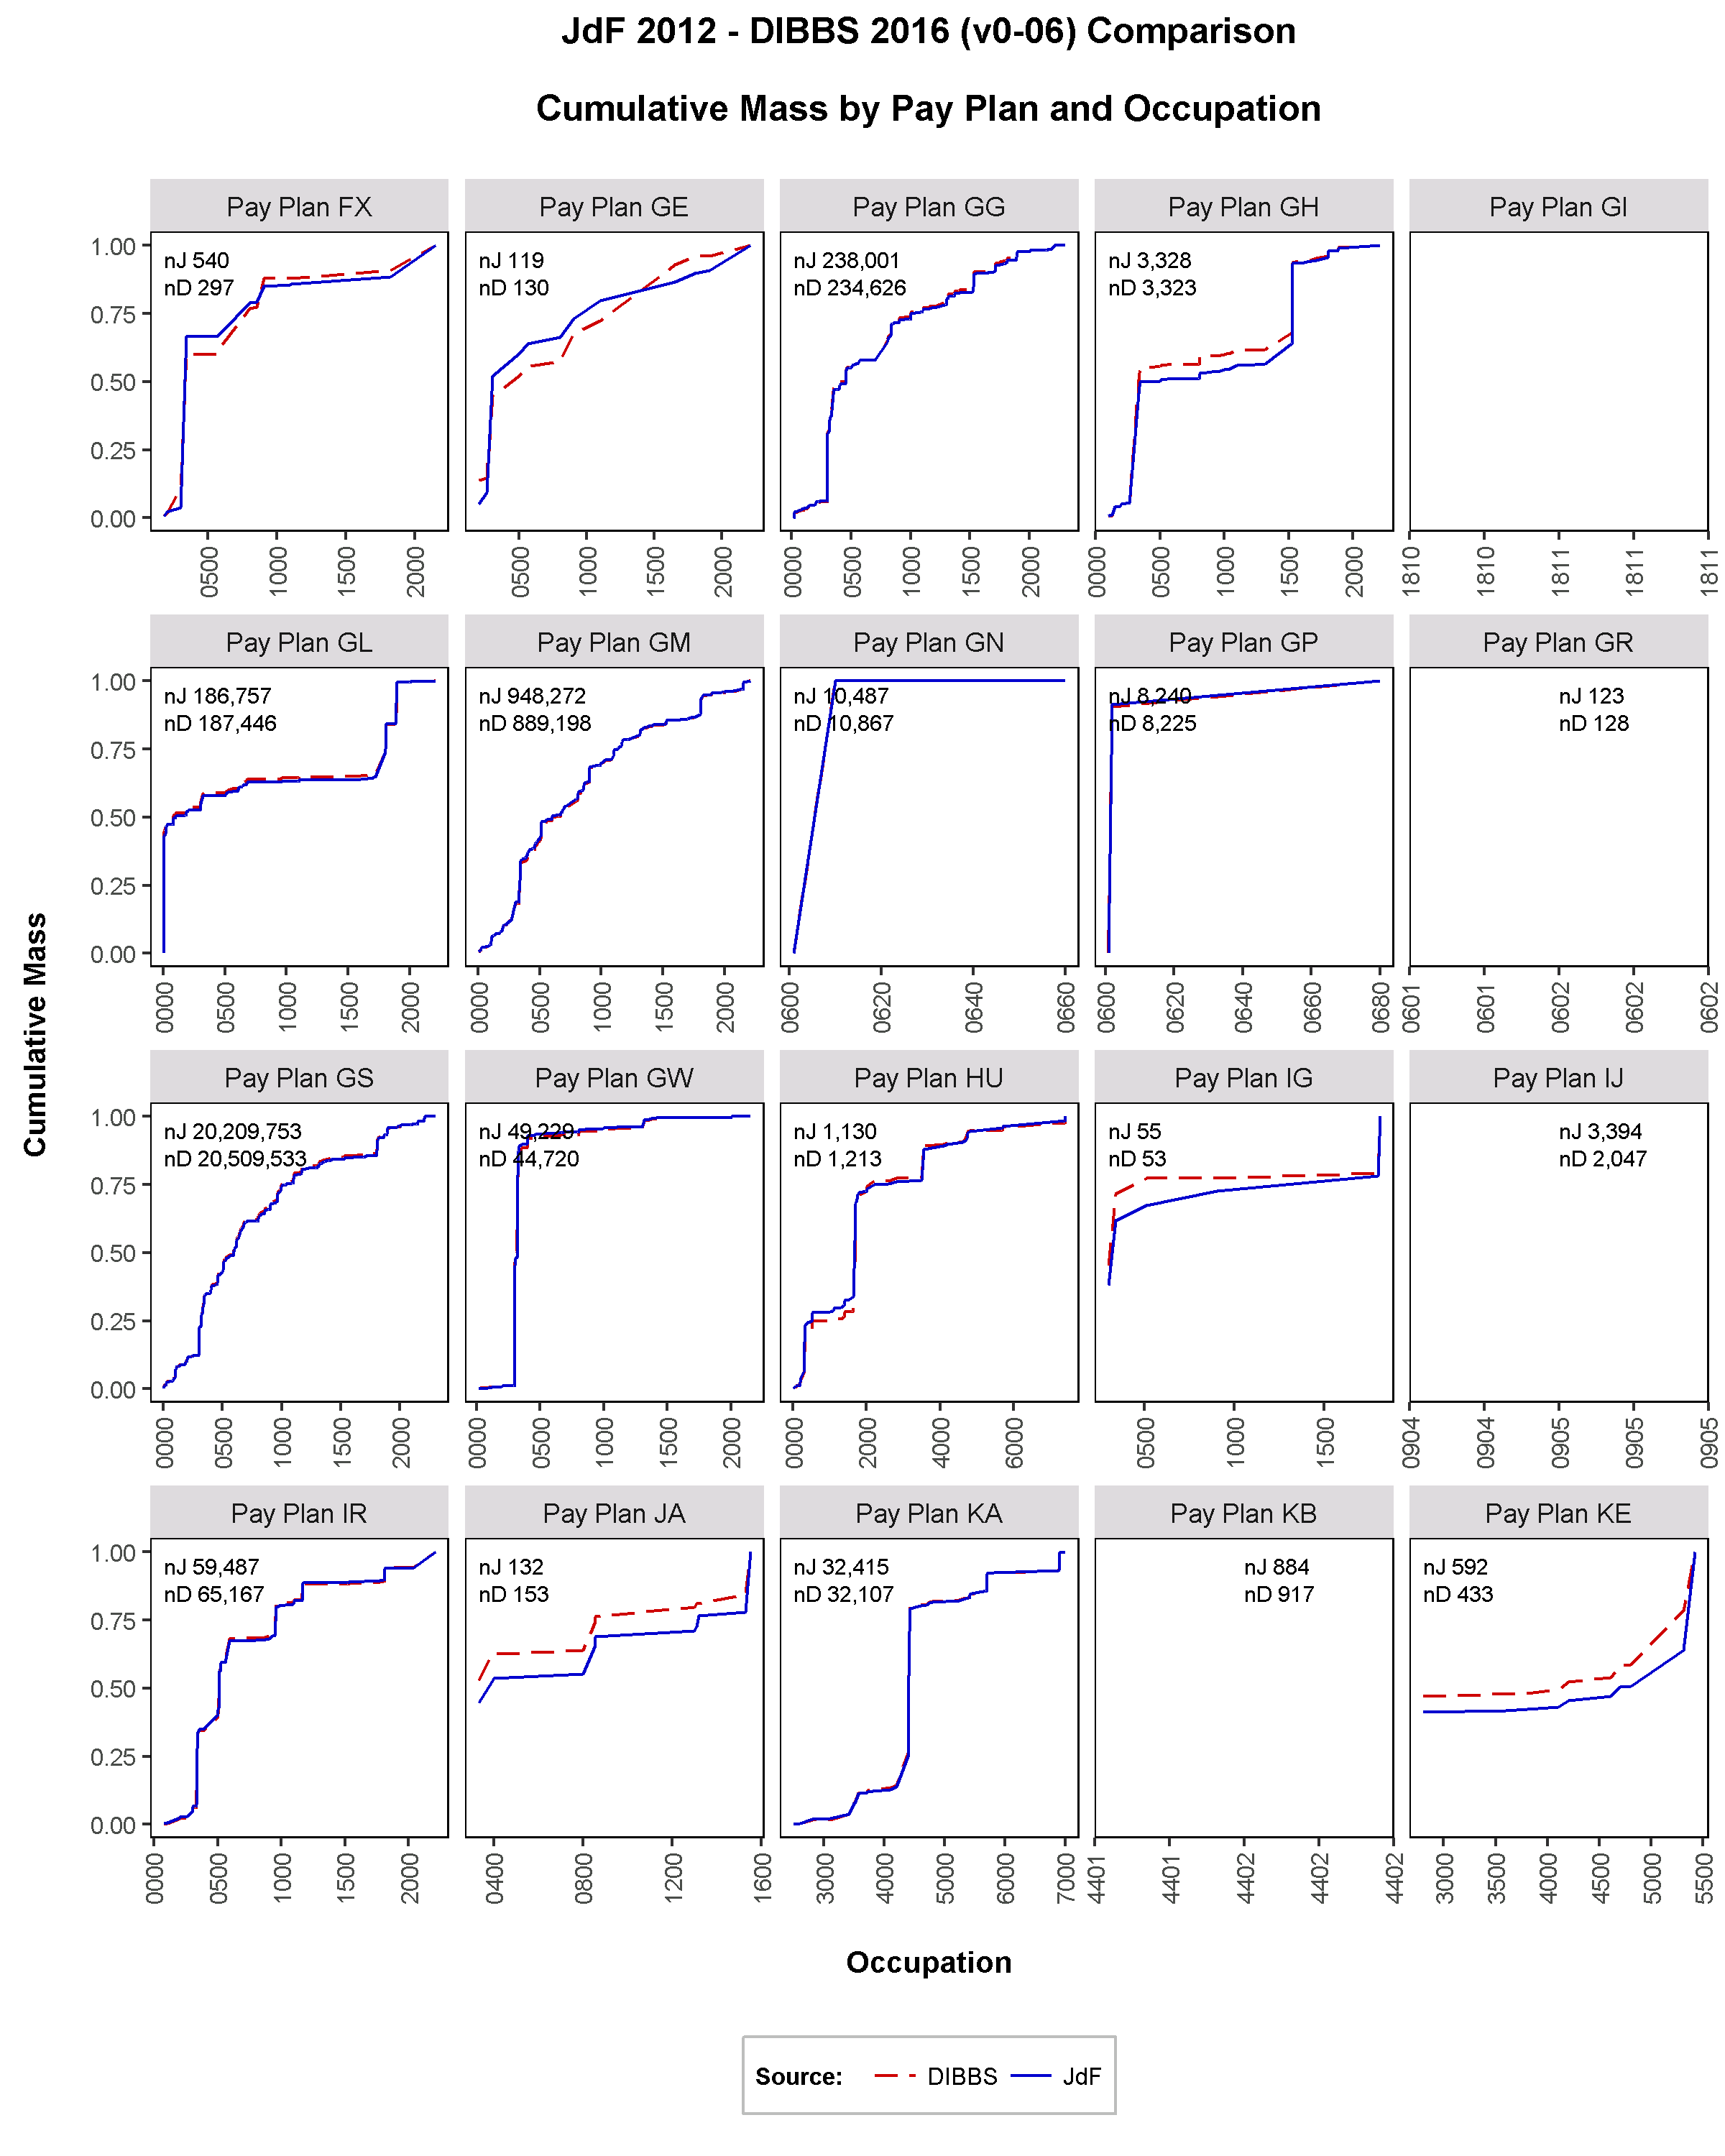
\includegraphics[width=5.9in, trim={0 0 0 0.75in}, clip]{CMFOccupationPayPlan61.png}
    \caption{Cumulative mass by occupation within pay plan.  Pay plan set one.}
    \label{figure:CMFOccupationPayPlan1}
\end{figure}

\begin{figure}[h!]
    \centering
    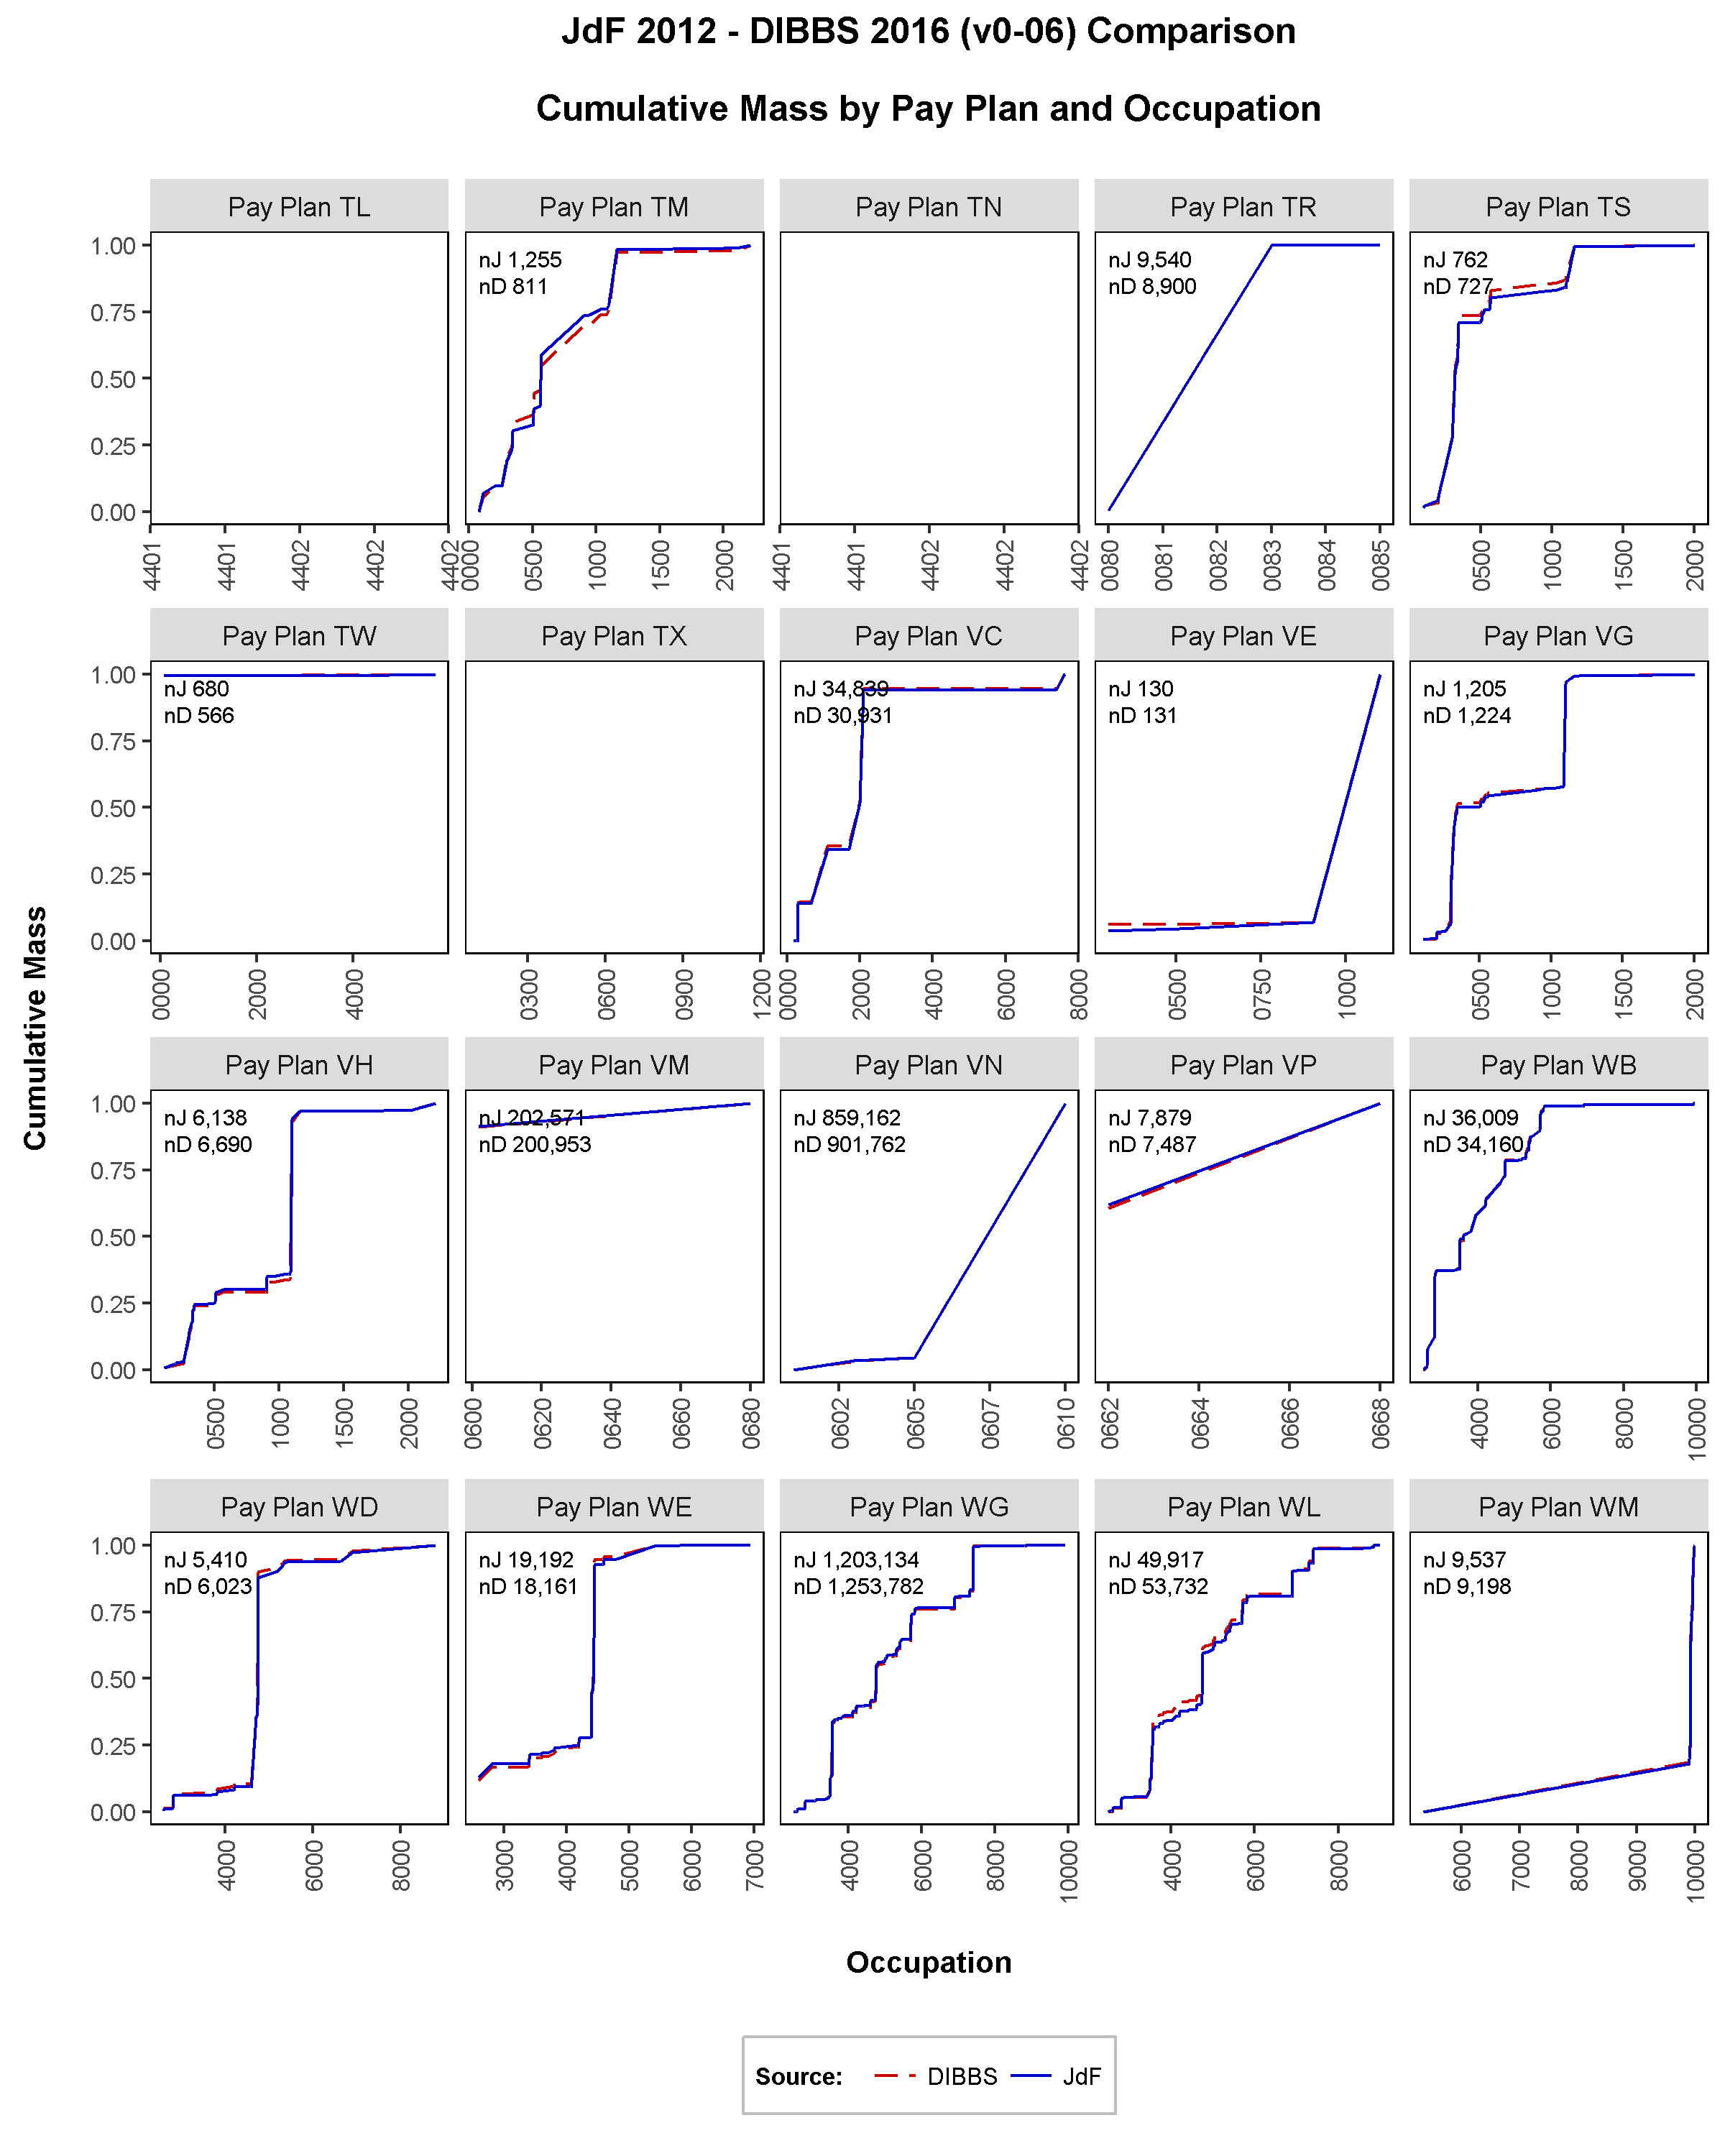
\includegraphics[width=5.9in, trim={0 0 0 0.75in}, clip]{CMFOccupationPayPlan141.png}
    \caption{Cumulative mass by occupation within pay plan.  Pay plan set 2.}
    \label{figure:CMFOccupationPayPlan2}
\end{figure}

\clearpage

DISTRIBUTION OF BASIC PAY BY AGENCY\\

Basic pay is an important dependent study variable and the distribution of pay values in the authentic data must be maintained in the synthetic data.  Figure \ref{figure:JdFDIBBSBasicPayDistribution} plots the distribution of basic pay for the top eight frequency agencies (first two positions):  Department of Agriculture (AG), Department of Justice (DJ), Department of Health and Human Services (HE), Department of Homeland Security (HS), Department of Interior (IN), Department of Transportation (TD), Department of Treasury (TR), and the Department of Veterans Affairs (VA).  These agencies account for approximately 85\% of observations.  Synthetic distribution represented by dashed line, authentic distribution by solid line.  ``n(D)" indicates synthetic data observation frequency, ``n(J)" indicates authentic data observation count.\\

Observations:  Although each data set is represented in each graph, a single striped-appearing line is visible, due to identical frequency proportions at each pay level.  Local increases, decreases, and trends in authentic distribution are accurately represented in the synthetic data. 

\vspace{12pt}

\begin{figure}[h]
    \centering
    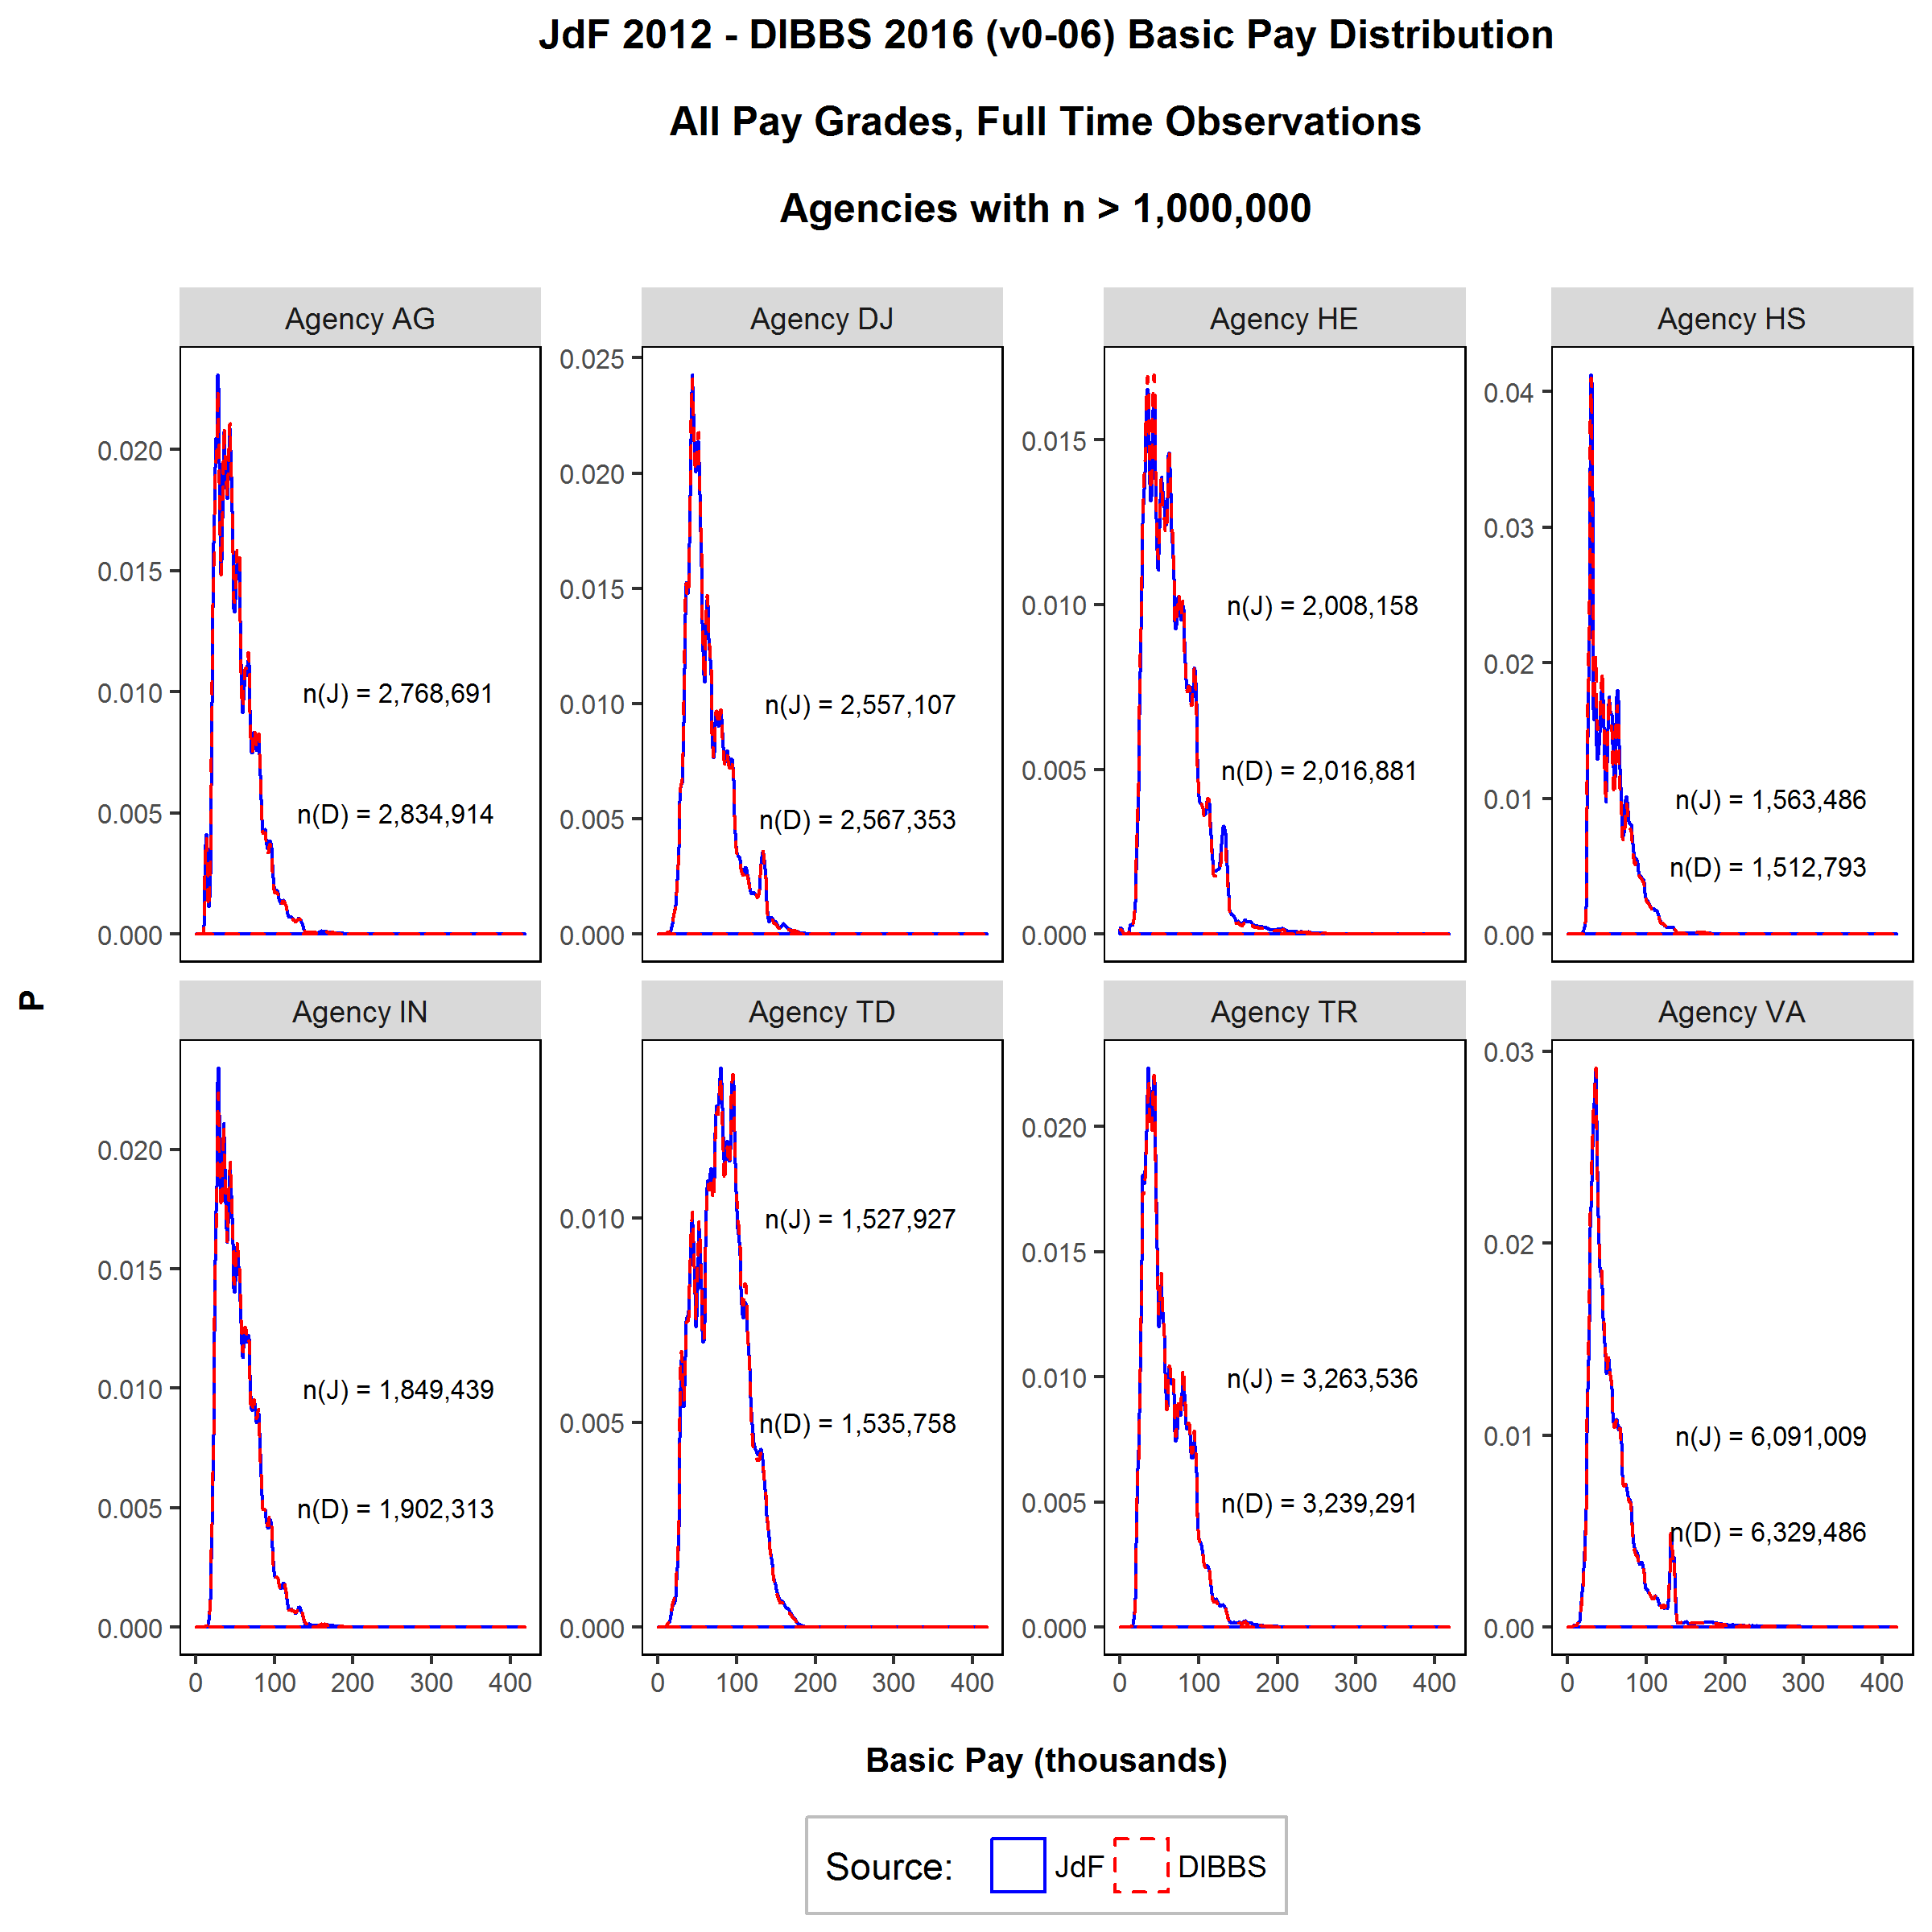
\includegraphics[width=6in, trim={0 0 1in 1in}, clip]{JdFDIBBSBasicPayDistribution.png}
    \caption{Basic pay marginal distribution for top eight agencies.  Dashed line for synthetic data, solid line for authentic.}
    \label{figure:JdFDIBBSBasicPayDistribution}
\end{figure}

\clearpage

DISTRIBUTION OF BASIC PAY BY PROFESSIONAL, SUPERVISORY, COLLEGE EDUCATION, AND WORK SCHEDULE CATEGORY\\

Professional classification, supervisory status, and college education are important independent variables in human capital research.  Figures \ref{figure:JdFDIBBSBasicPayCDFAG} through \ref{figure:JdFDIBBSBasicPayCDFVA} plot, for the top eight frequency agencies, the distribution of basic pay by these independent variables and work schedule code.  One column for each professional, supervisory, college combination (column code position one equals ``P" if occupational category is administrative or professional, position two equals ``S" if supervisory status is enabled, position three equals ``C" if education level at or above college).  One row for each work schedule code [significant codes are full time (F), full time seasonal (G), intermittent (I), intermittent seasonal (J), and part time (P)].  Synthetic distribution indicated by dashed line, authentic distribution by solid line.  ``n(D)" indicates synthetic data observation frequency, ``n(J)" indicates authentic data observation count.\\

Observations:  There exists near identical distribution for high frequency combinations, as indicated by striped, single line appearance due to overlay of synthetic on authentic lines.  Slight differences in distribution are observed for small frequency combinations.

\vspace{12pt}

\begin{figure}[h]
    \centering
    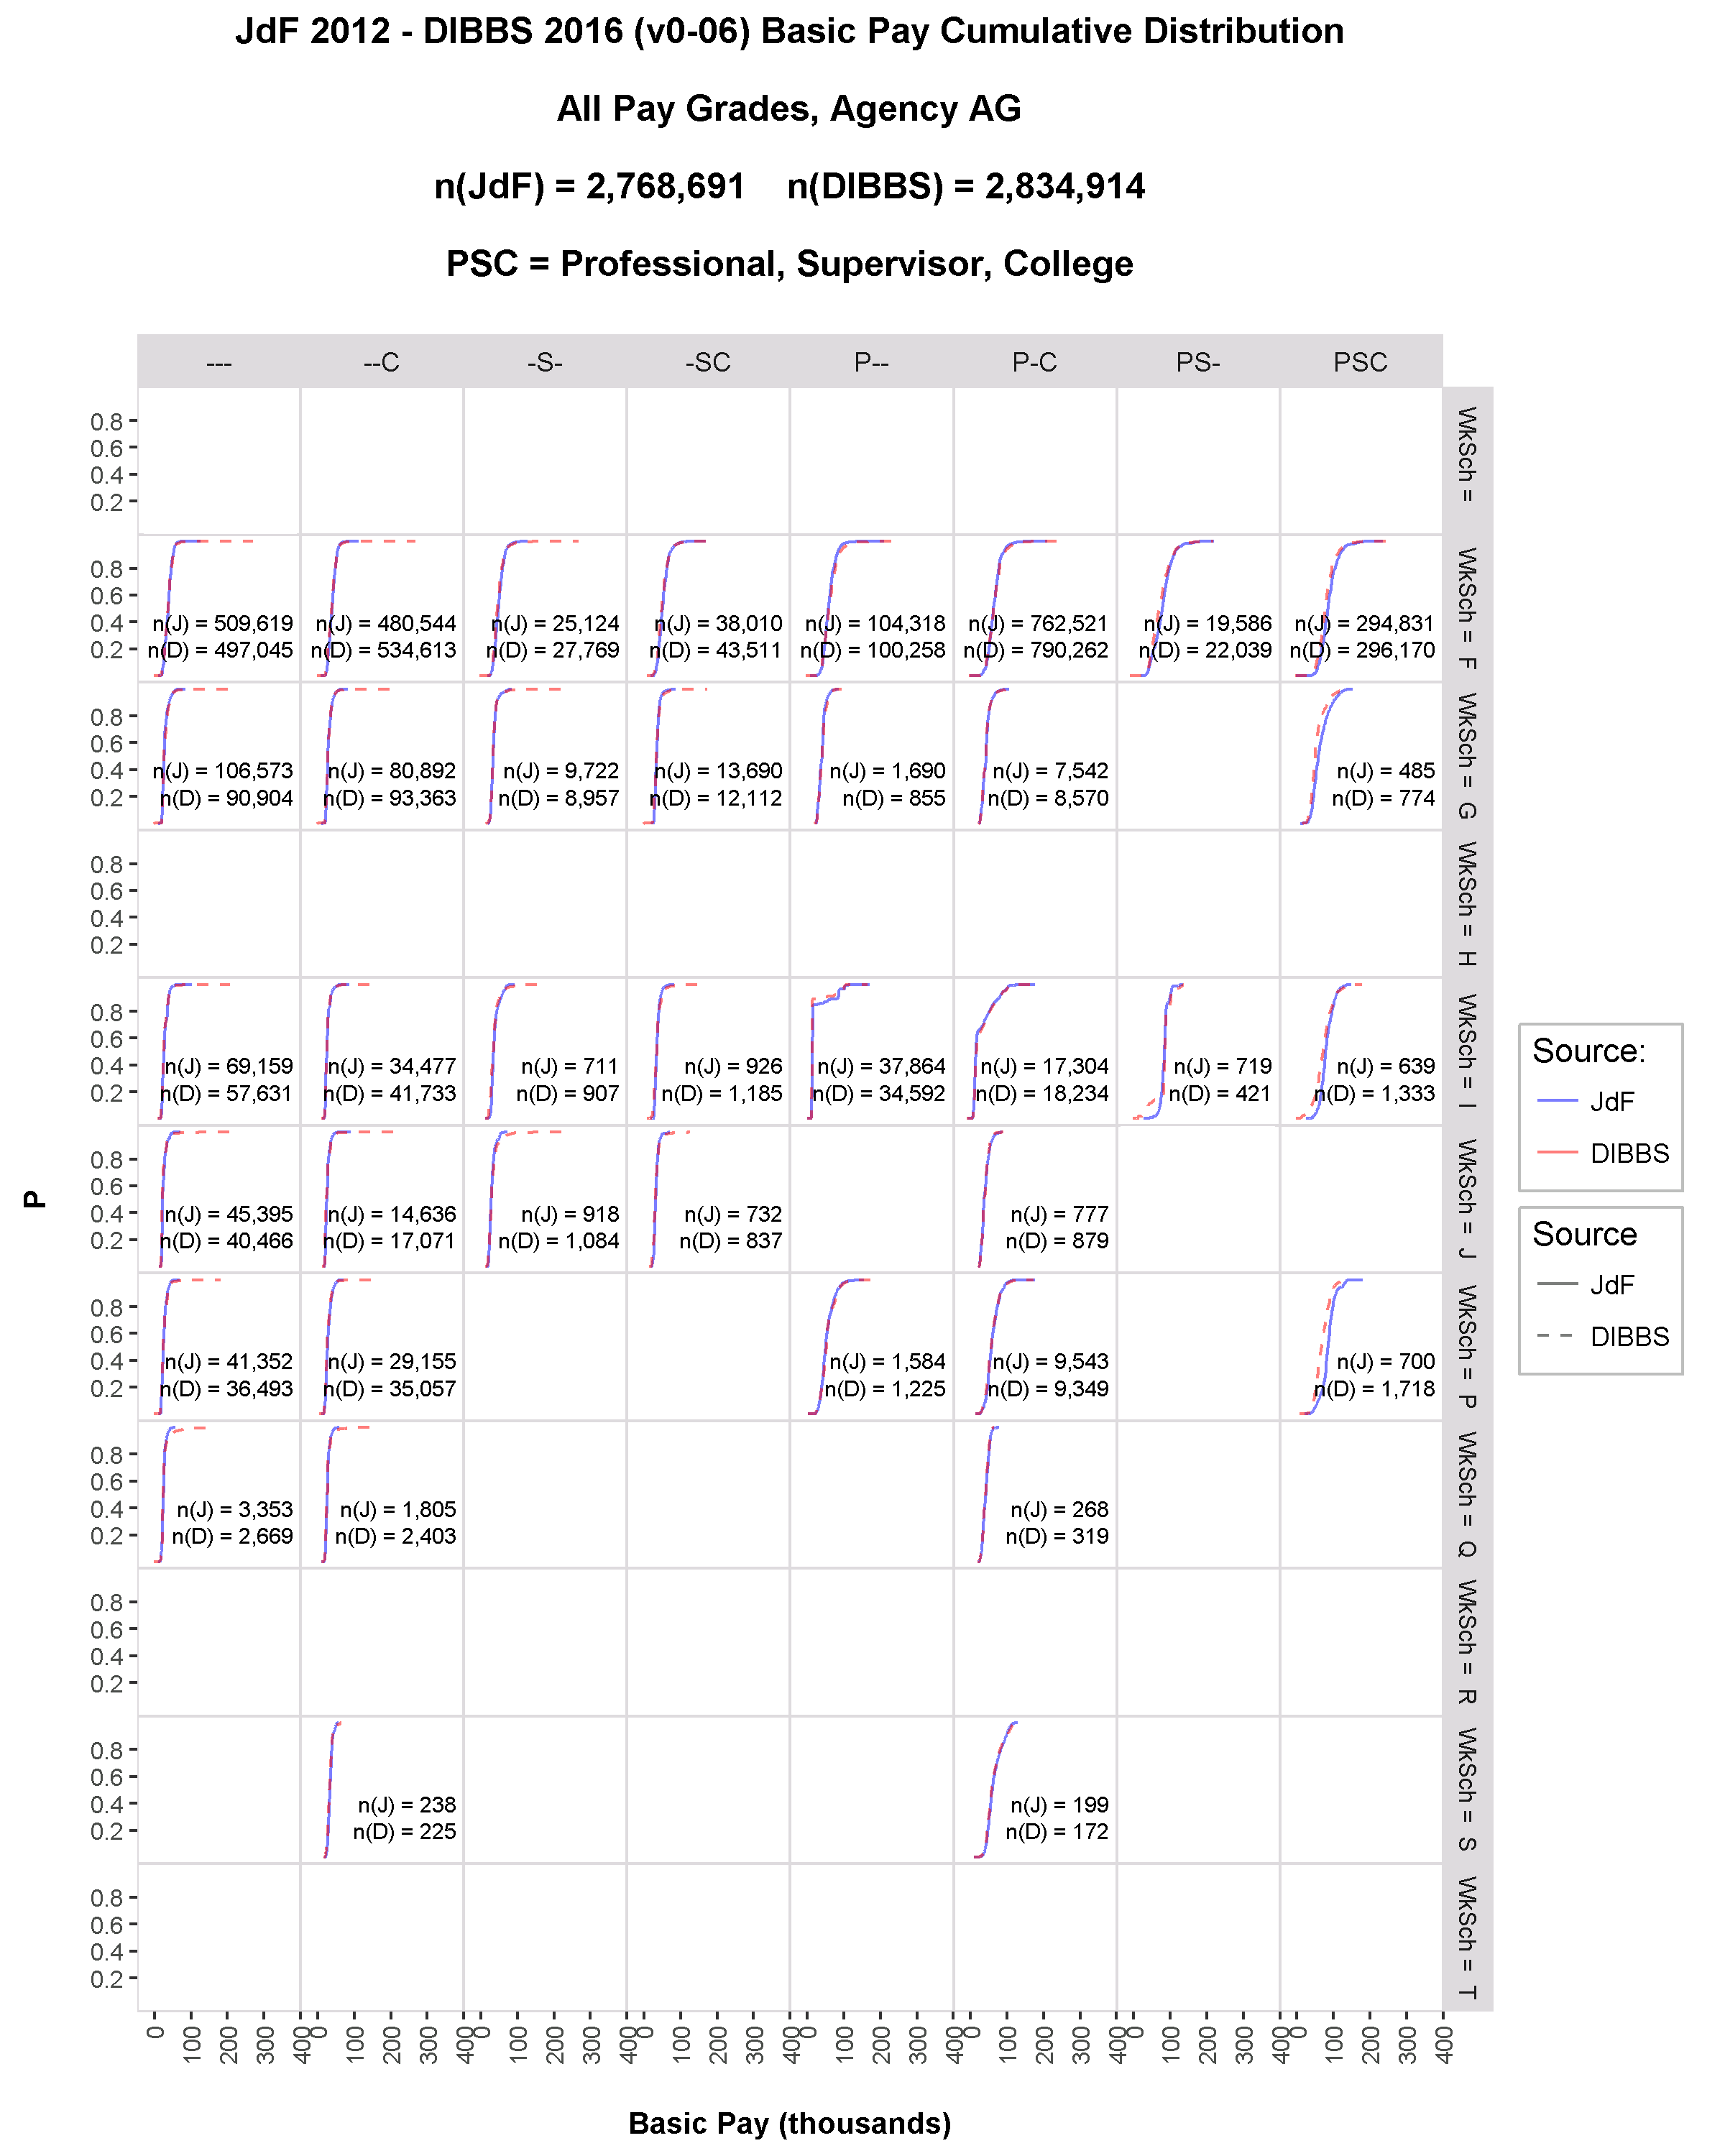
\includegraphics[width=6.5in, trim={0 0 1in 1.5in}, clip]{JdFDIBBSBasicPayCDFAG.png}
    \caption{Basic pay distribution by joint professional, supervisory status, college education, and work schedule  categories.  Department of Agriculture (AG).  Dashed line for synthetic data, solid line for authentic.}
    \label{figure:JdFDIBBSBasicPayCDFAG}
\end{figure}

\clearpage

\begin{figure}[h]
    \centering
    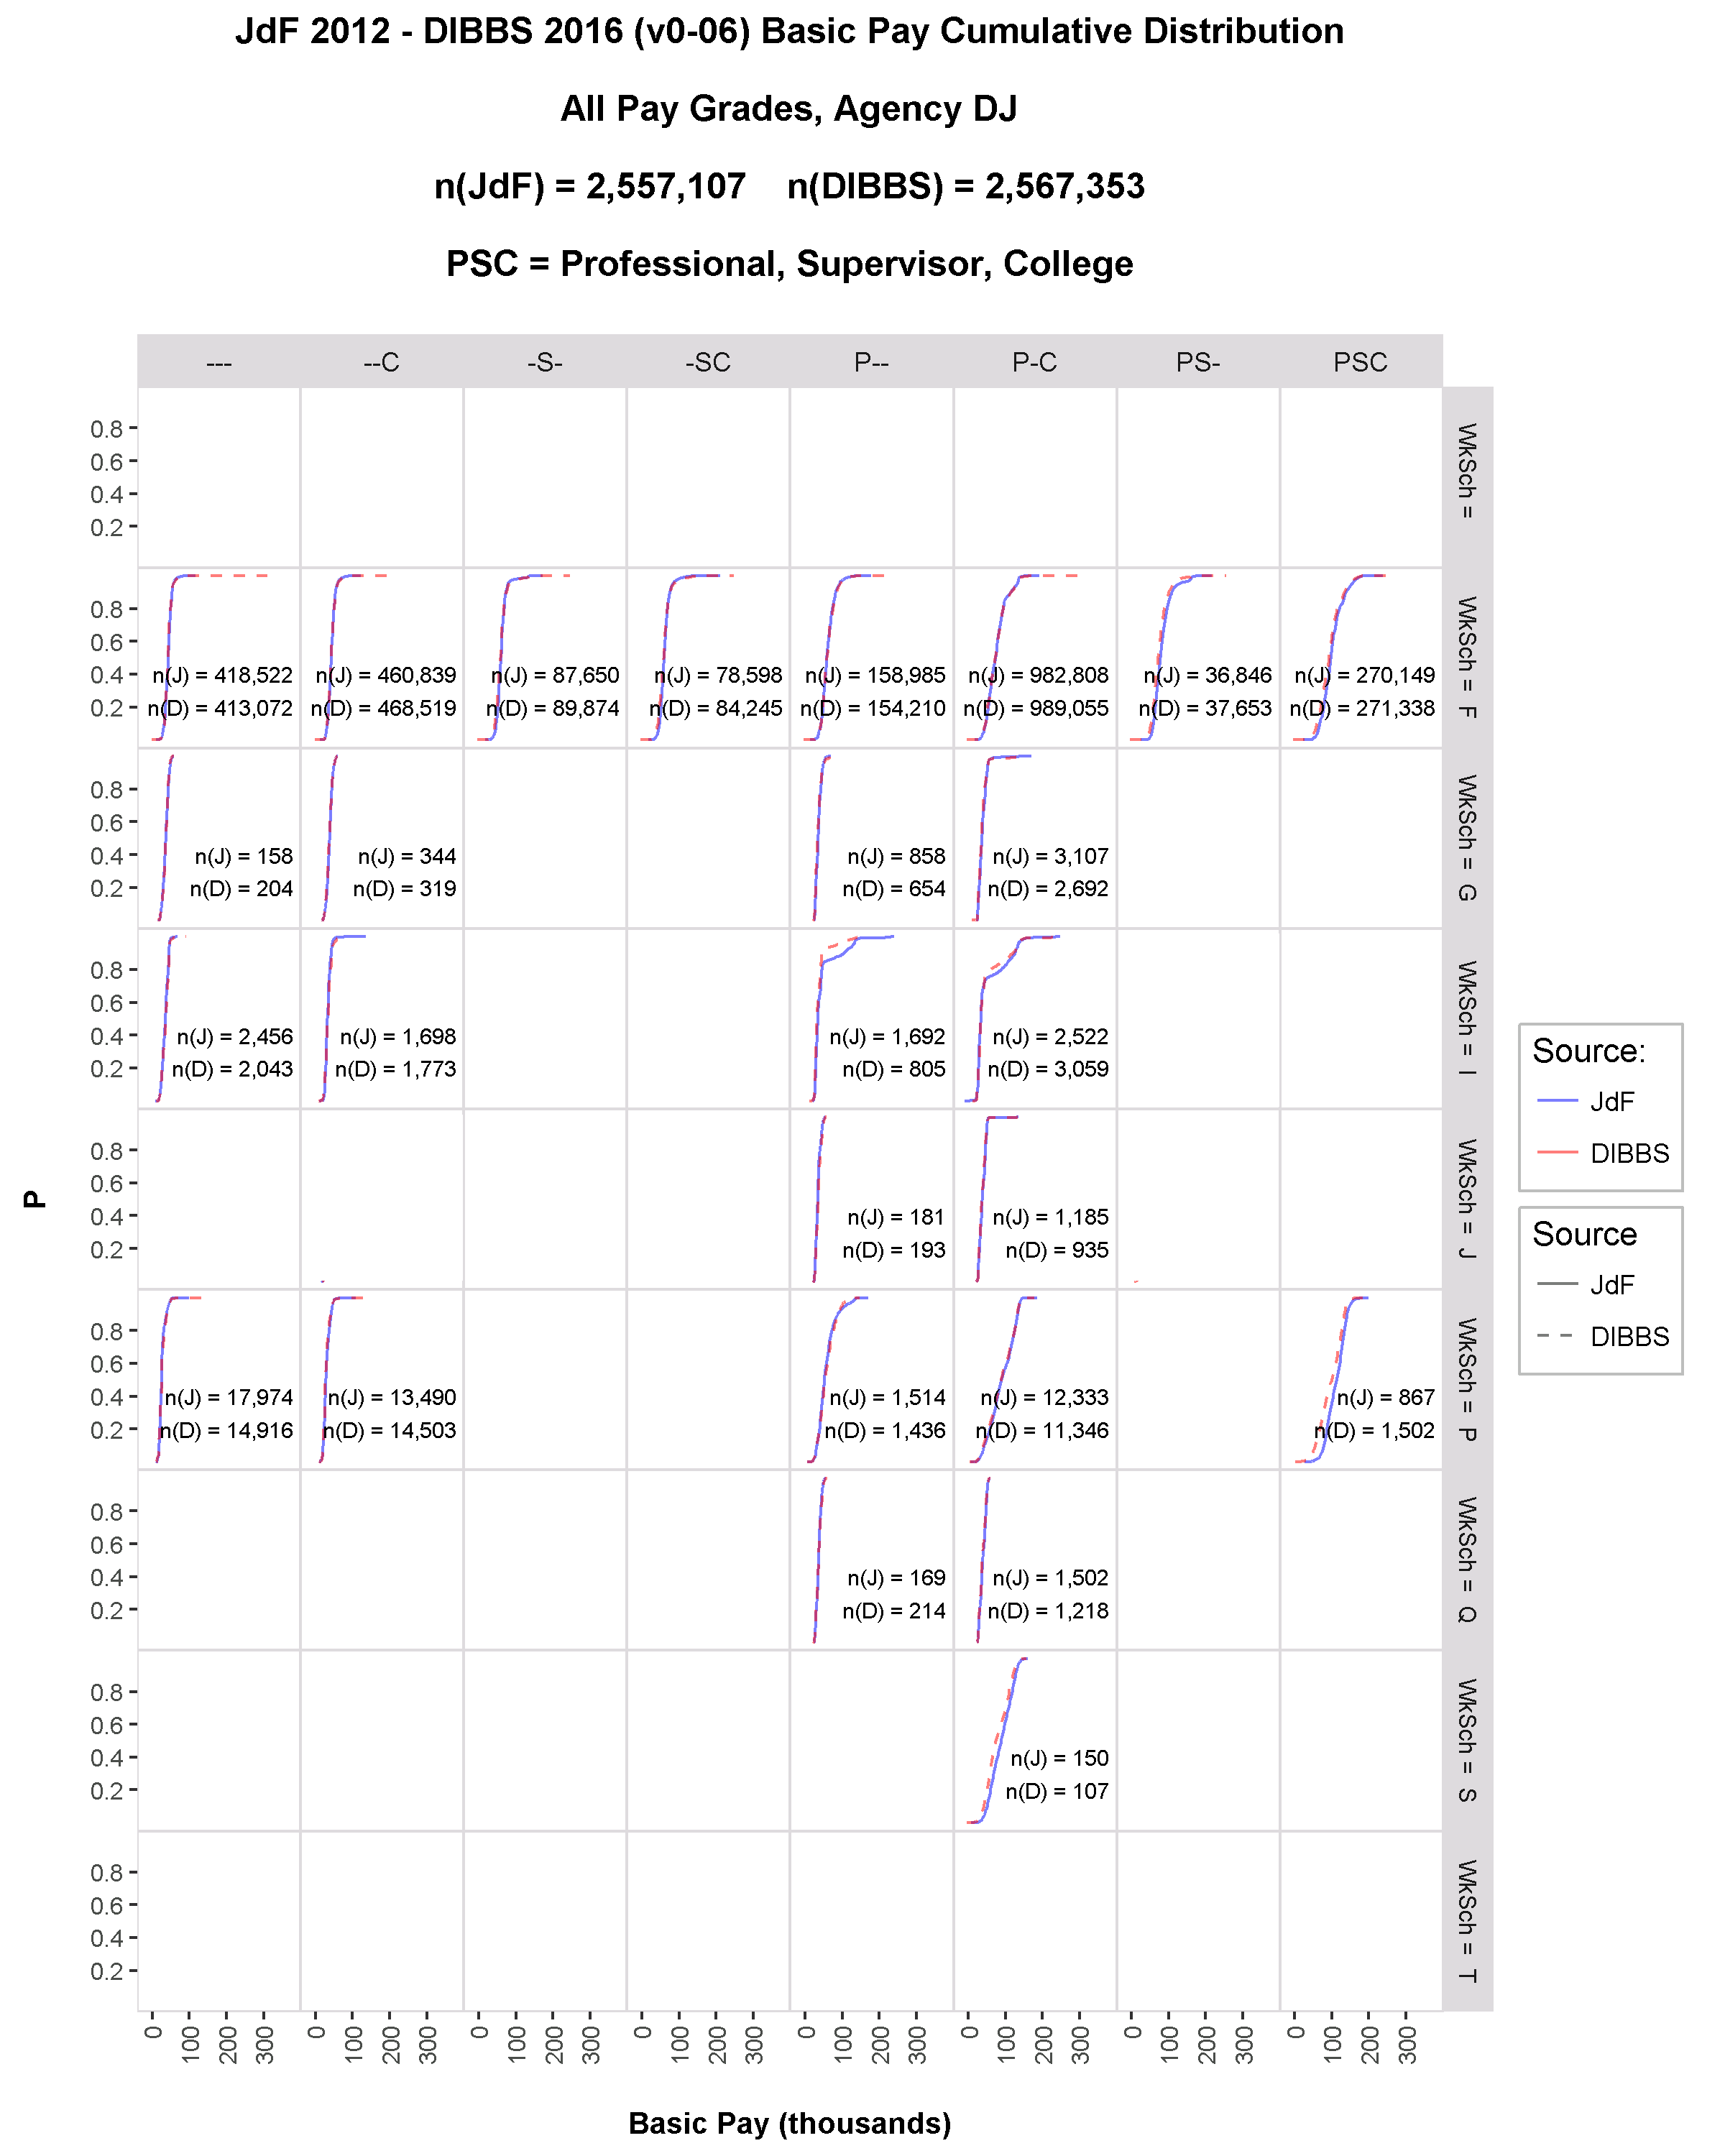
\includegraphics[width=6.5in, trim={0 0 1in 1.5in}, clip]{JdFDIBBSBasicPayCDFDJ.png}
    \caption{Basic pay distribution by joint professional, supervisory status, college education, and work schedule  categories.  Department of Justice (DJ).  Dashed line for synthetic data, solid line for authentic.}
    \label{figure:JdFDIBBSBasicPayCDFDJ}
\end{figure}

\clearpage

\begin{figure}[h]
    \centering
    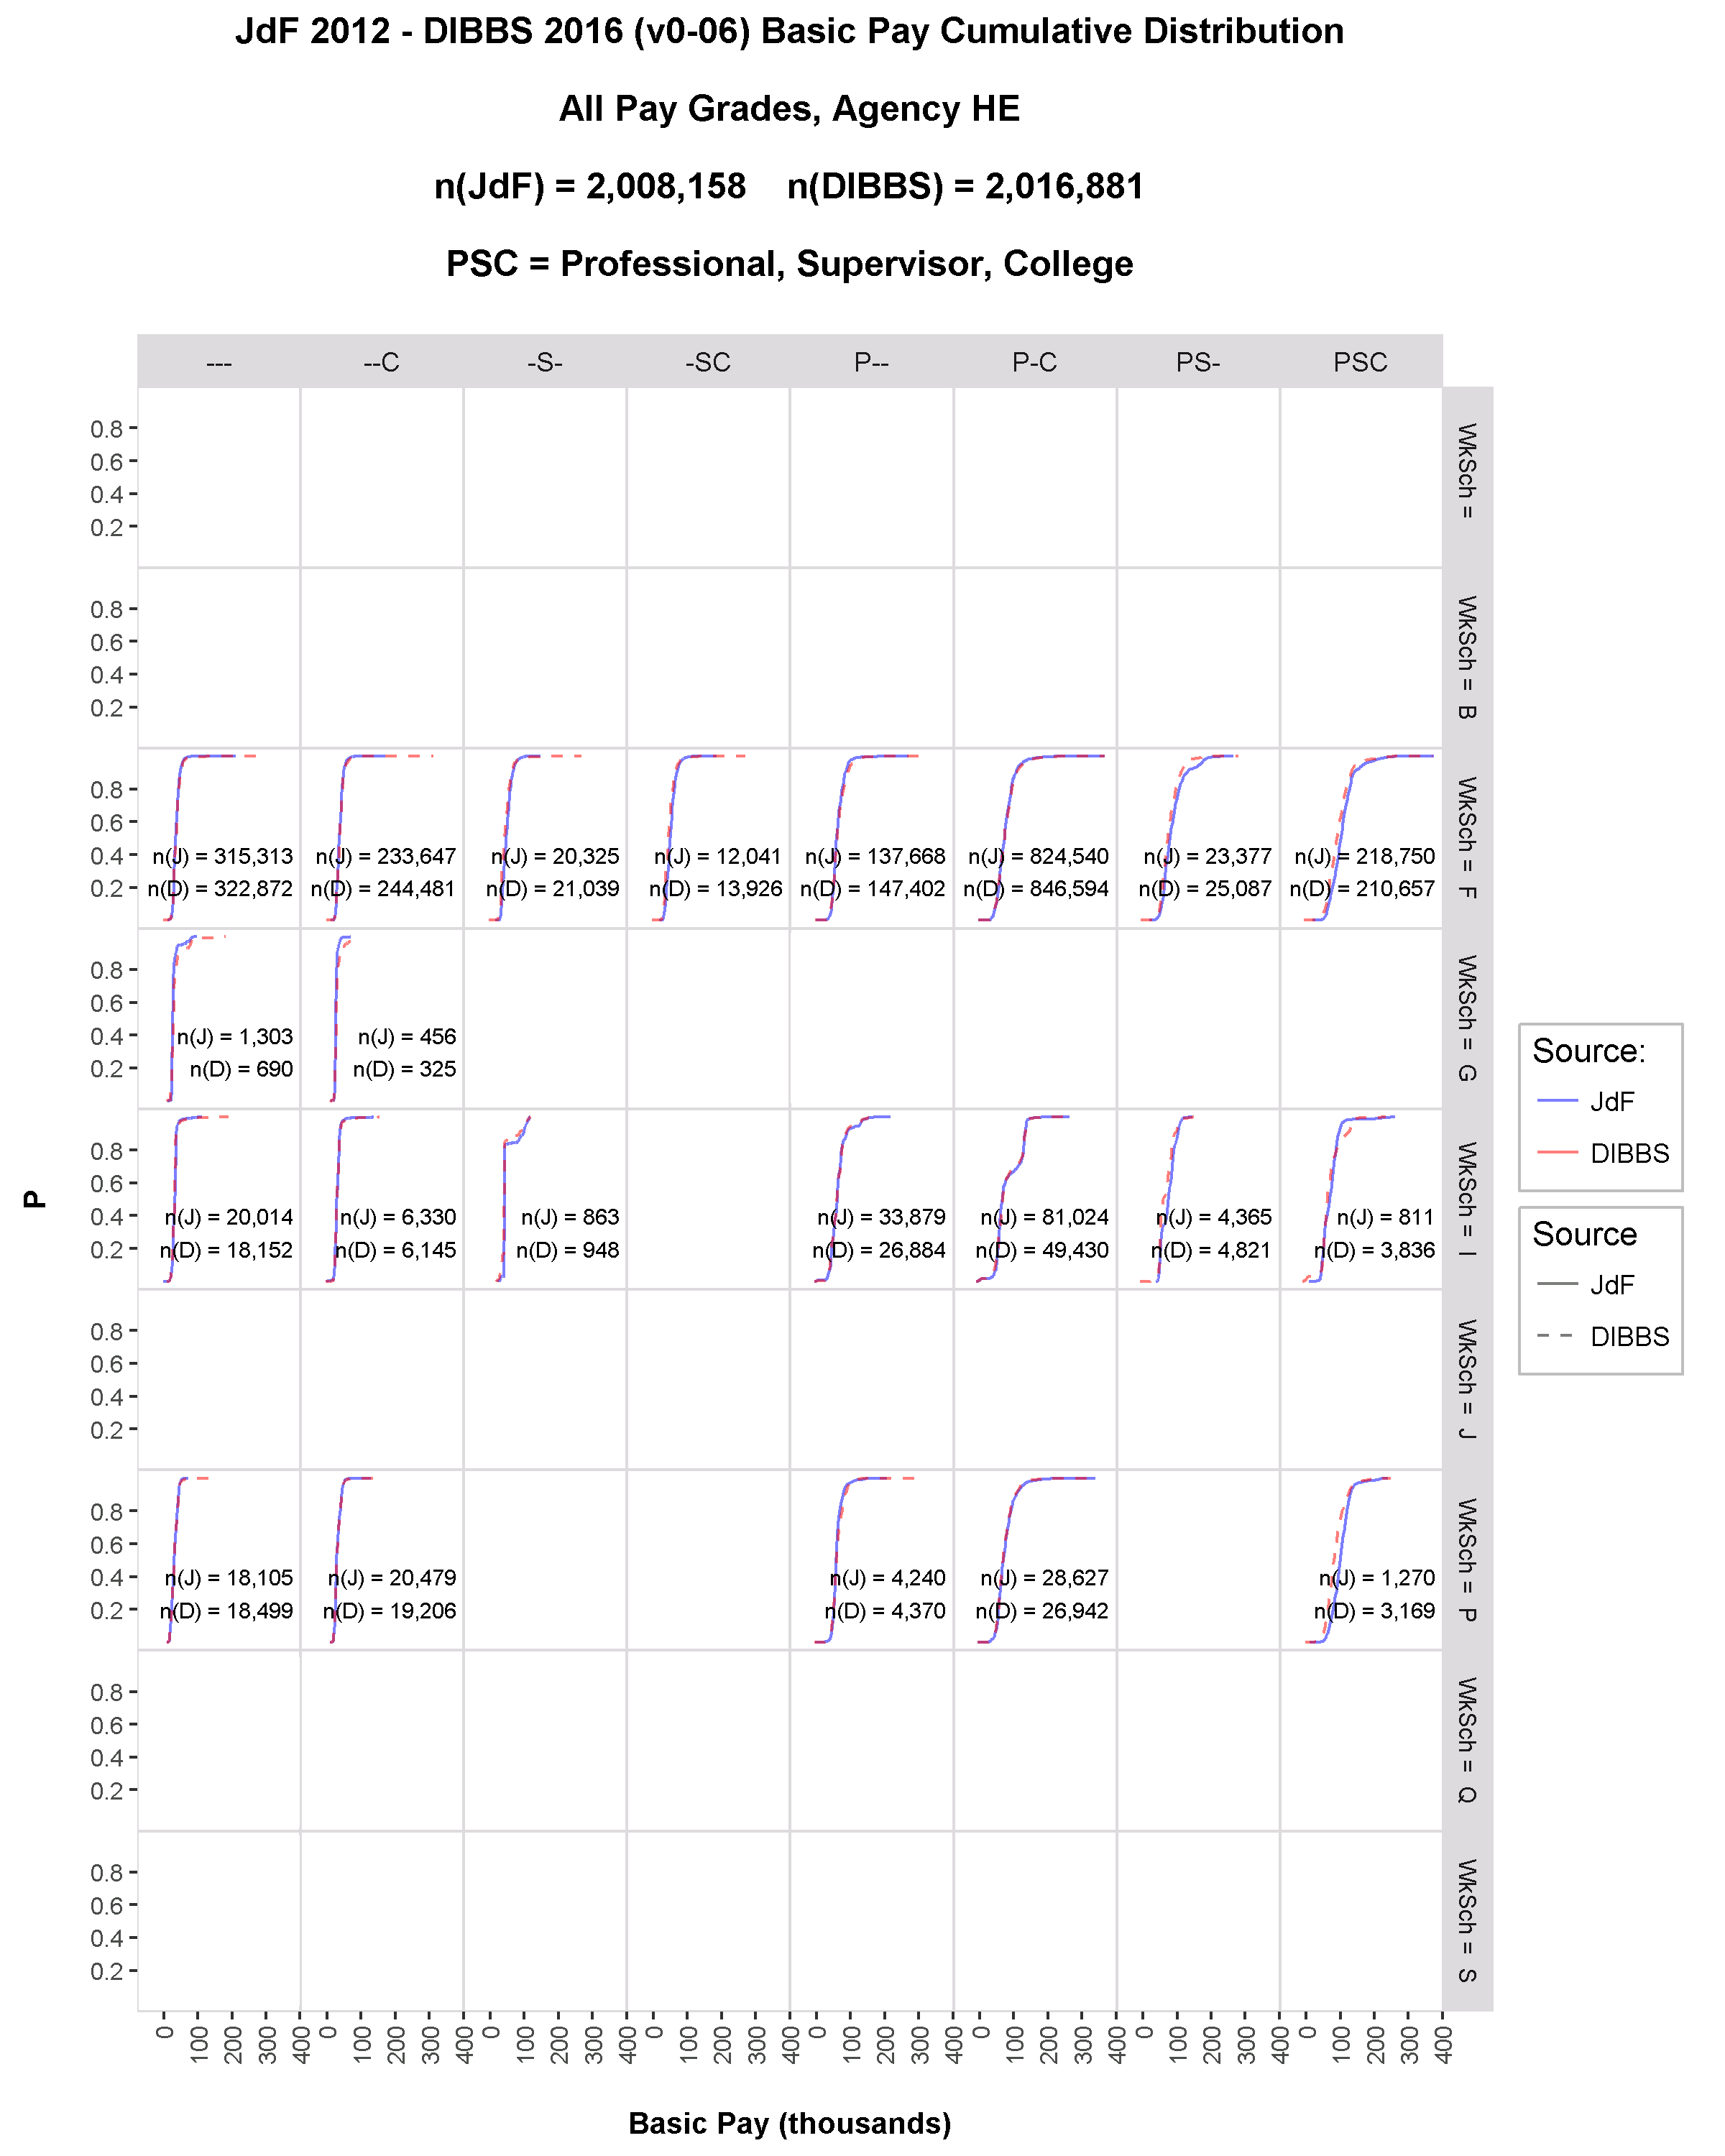
\includegraphics[width=6.5in, trim={0 0 1in 1.5in}, clip]{JdFDIBBSBasicPayCDFHE.png}
    \caption{Basic pay distribution by joint professional, supervisory status, college education, and work schedule  categories.  Department of Health and Human Services (HE).  Dashed line for synthetic data, solid line for authentic.}
    \label{figure:JdFDIBBSBasicPayCDFHE}
\end{figure}

\clearpage

\begin{figure}[h]
    \centering
    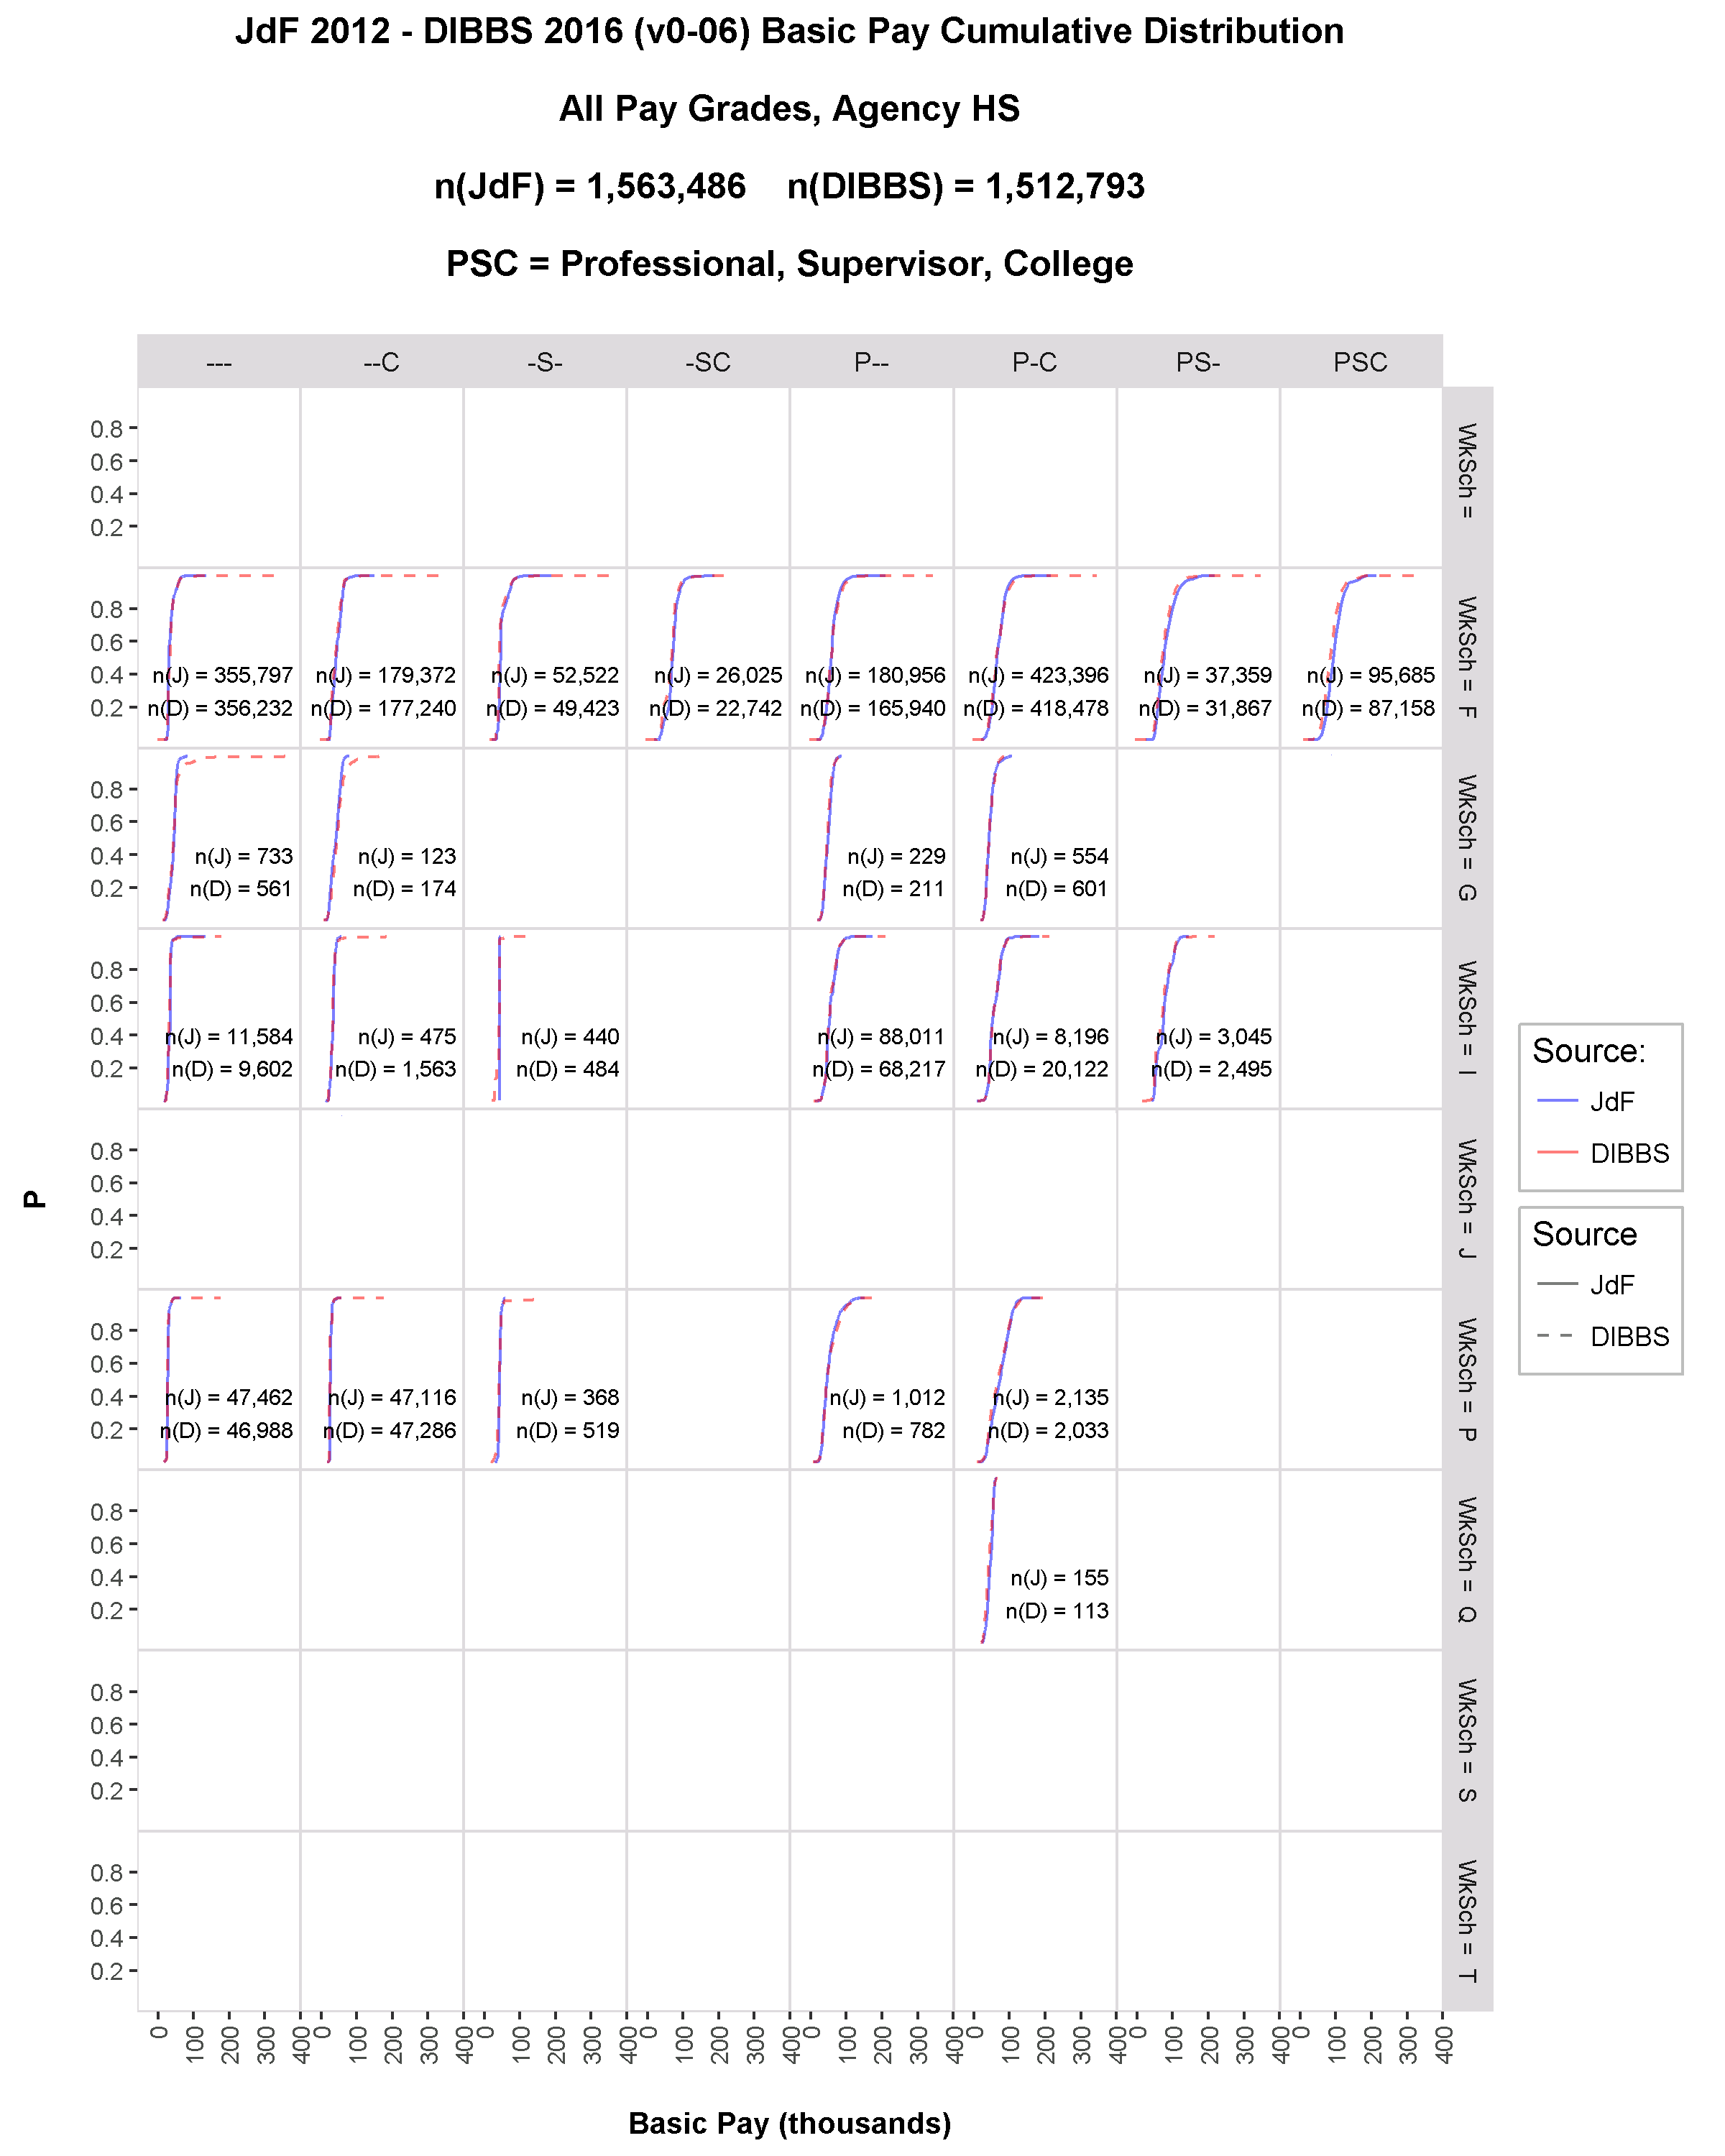
\includegraphics[width=6.5in, trim={0 0 1in 1.5in}, clip]{JdFDIBBSBasicPayCDFHS.png}
    \caption{Basic pay distribution by joint professional, supervisory status, college education, and work schedule  categories.  Department of Homeland Security (HS).  Dashed line for synthetic data, solid line for authentic.}
    \label{figure:JdFDIBBSBasicPayCDFHS}
\end{figure}

\clearpage

\begin{figure}[h]
    \centering
    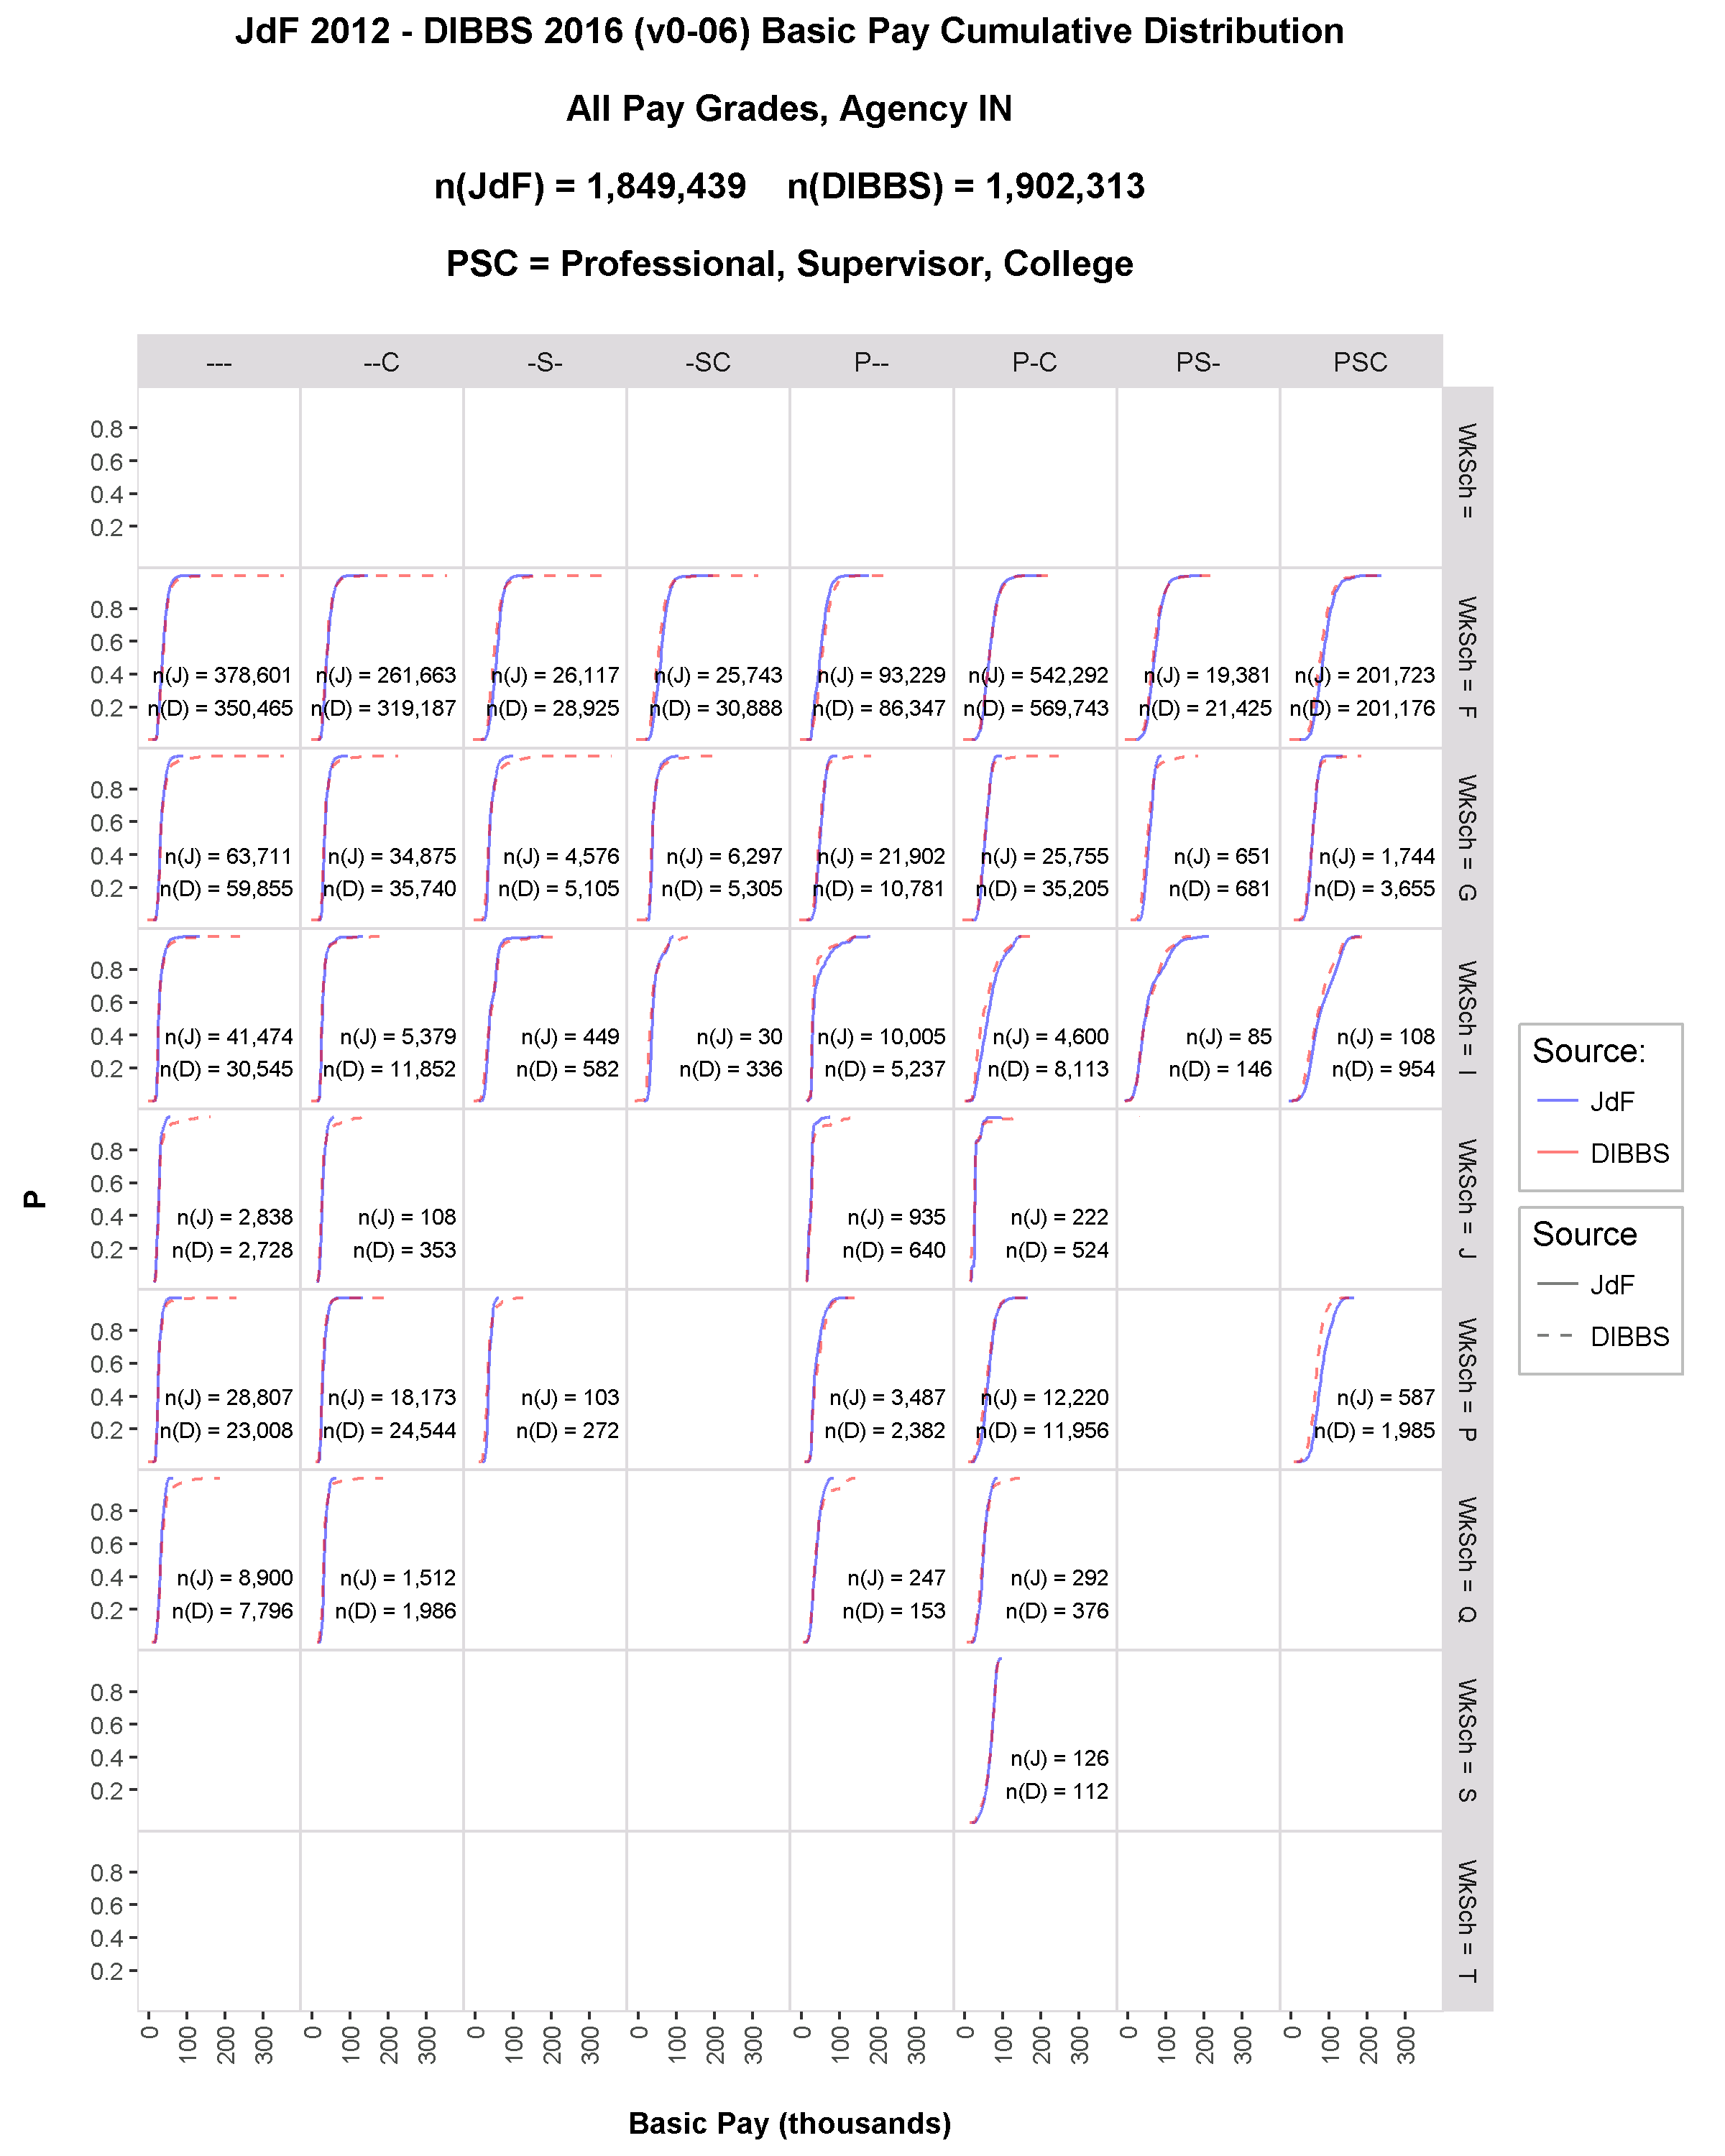
\includegraphics[width=6.5in, trim={0 0 1in 1.5in}, clip]{JdFDIBBSBasicPayCDFIN.png}
    \caption{Basic pay distribution by joint professional, supervisory status, college education, and work schedule  categories.  Department of Interior (IN).  Dashed line for synthetic data, solid line for authentic.}
    \label{figure:JdFDIBBSBasicPayCDFIN}
\end{figure}

\clearpage

\begin{figure}[h]
    \centering
    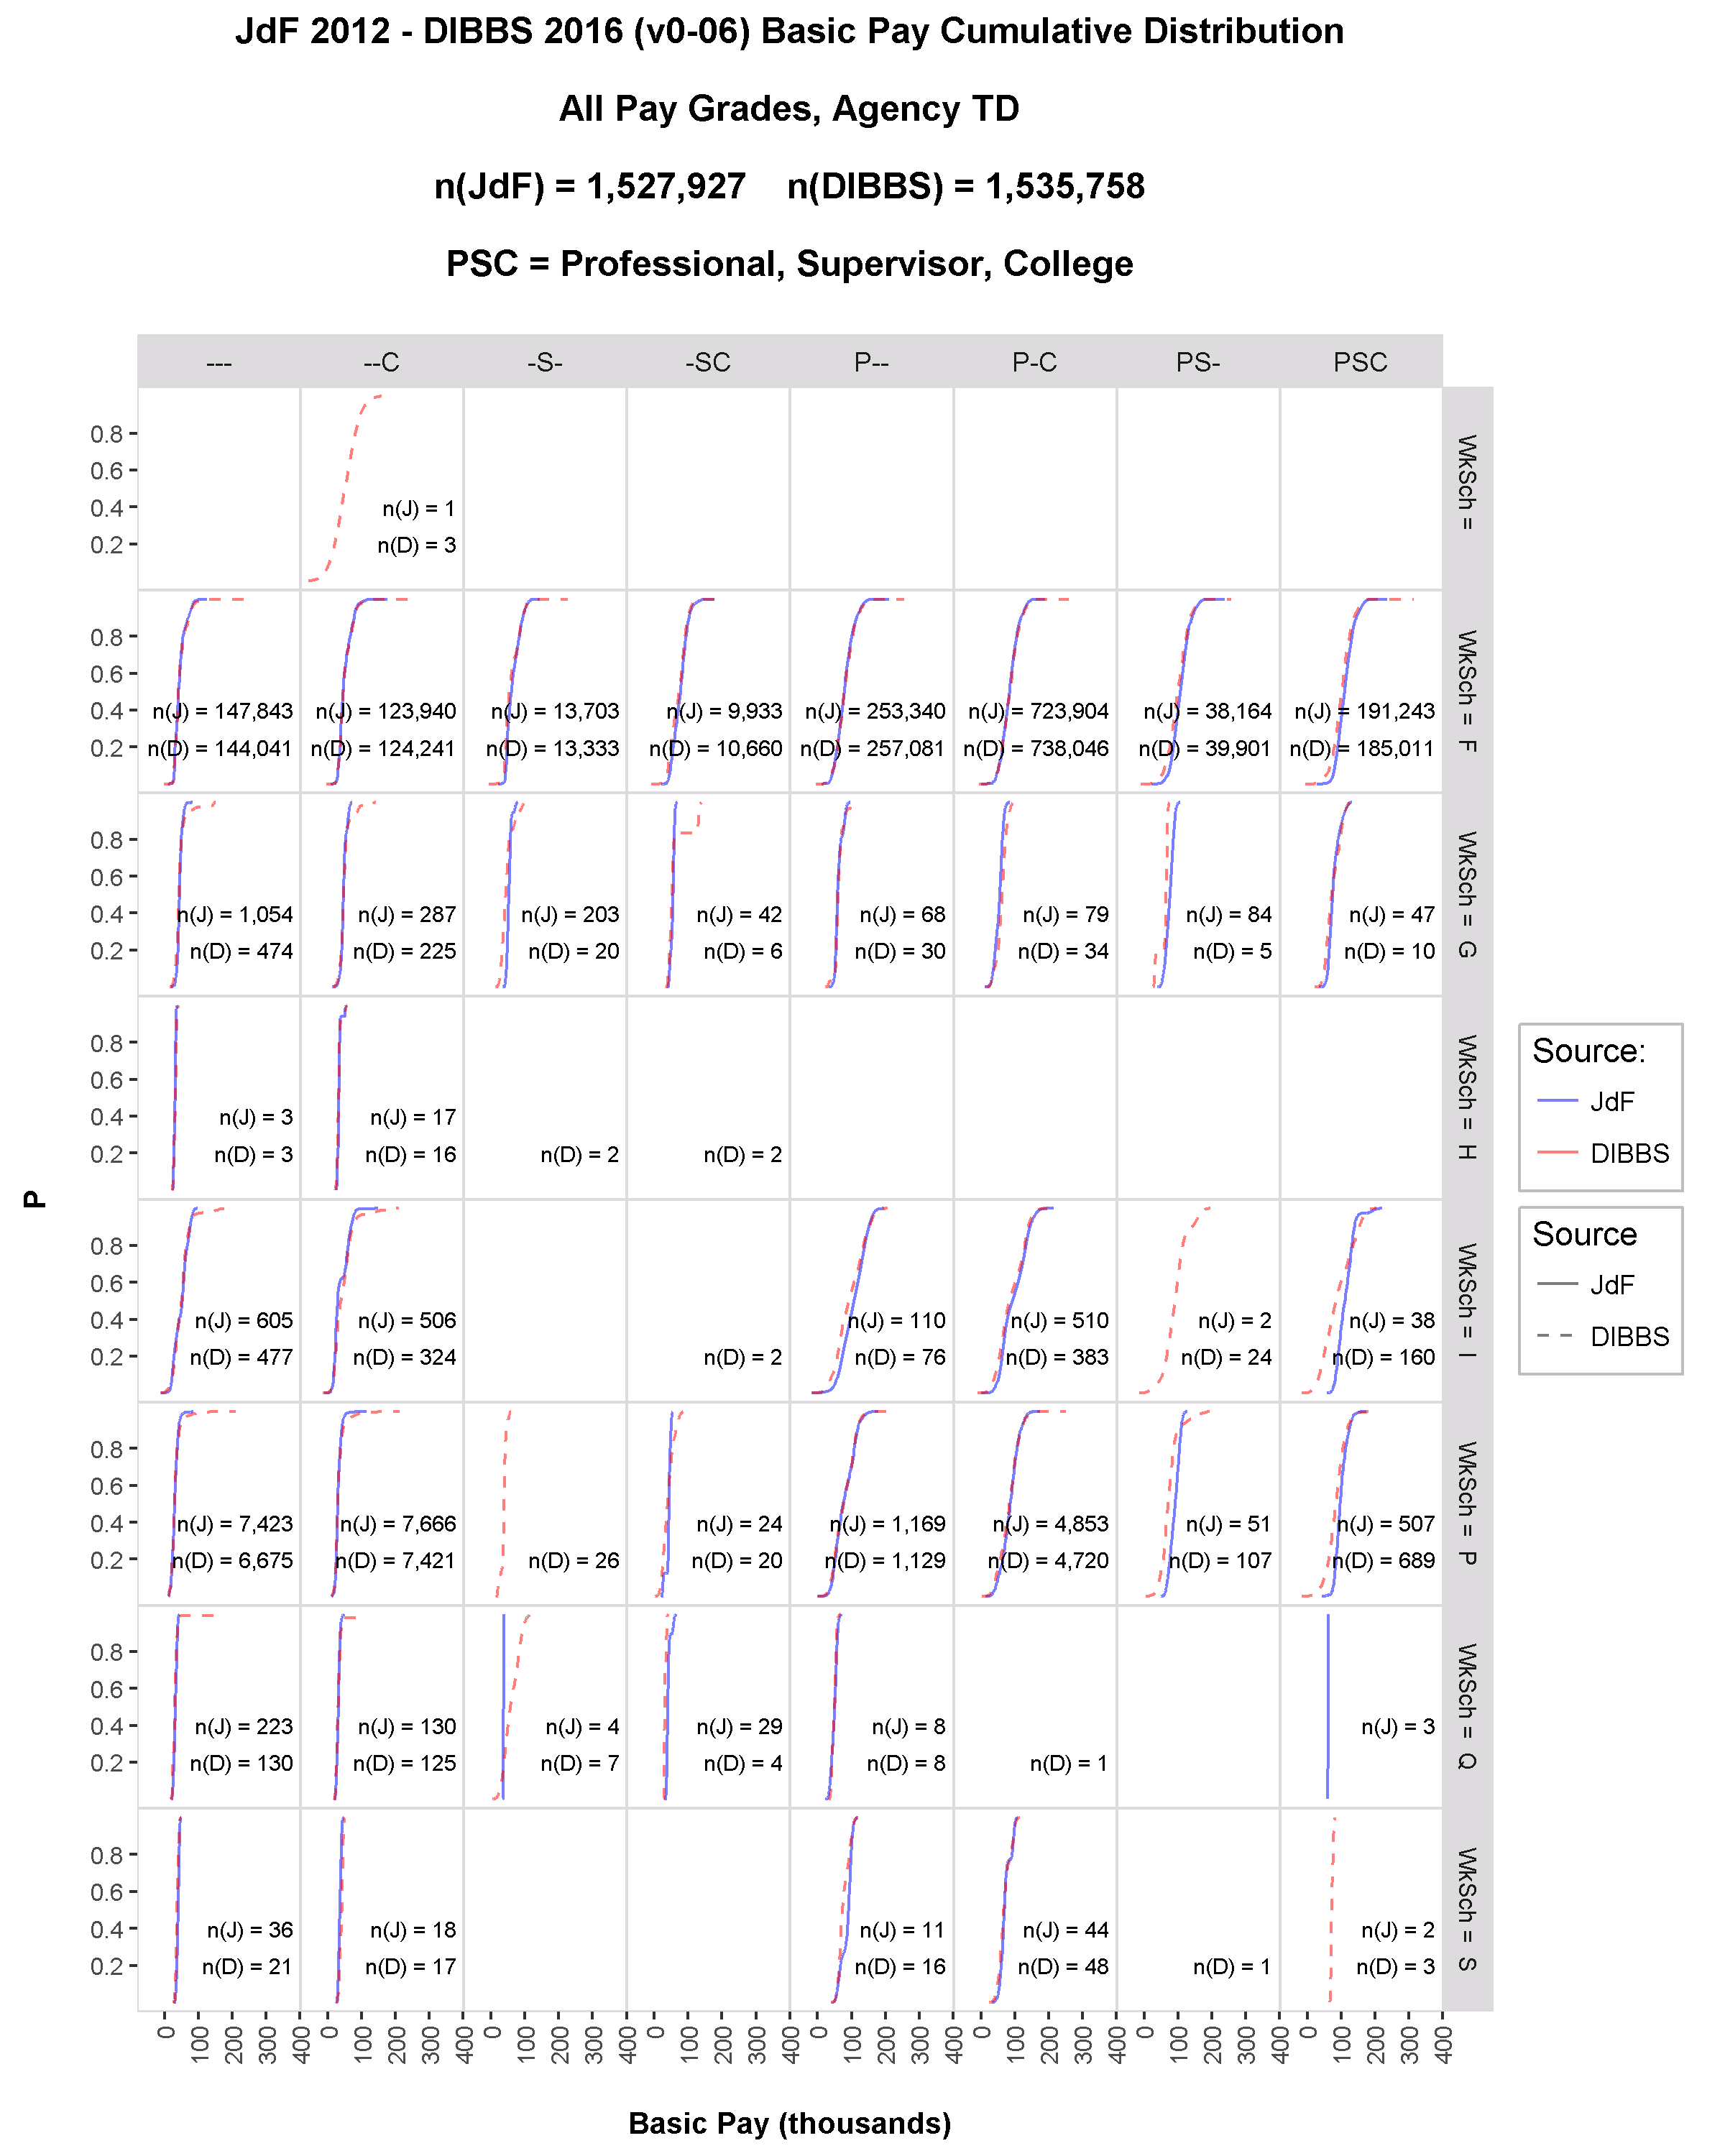
\includegraphics[width=6.5in, trim={0 0 1in 1.5in}, clip]{JdFDIBBSBasicPayCDFTD.png}
    \caption{Basic pay distribution by joint professional, supervisory status, college education, and work schedule  categories.  Department of Transportation (TD).  Dashed line for synthetic data, solid line for authentic.}
    \label{figure:JdFDIBBSBasicPayCDFTD}
\end{figure}

\clearpage

\begin{figure}[h]
    \centering
    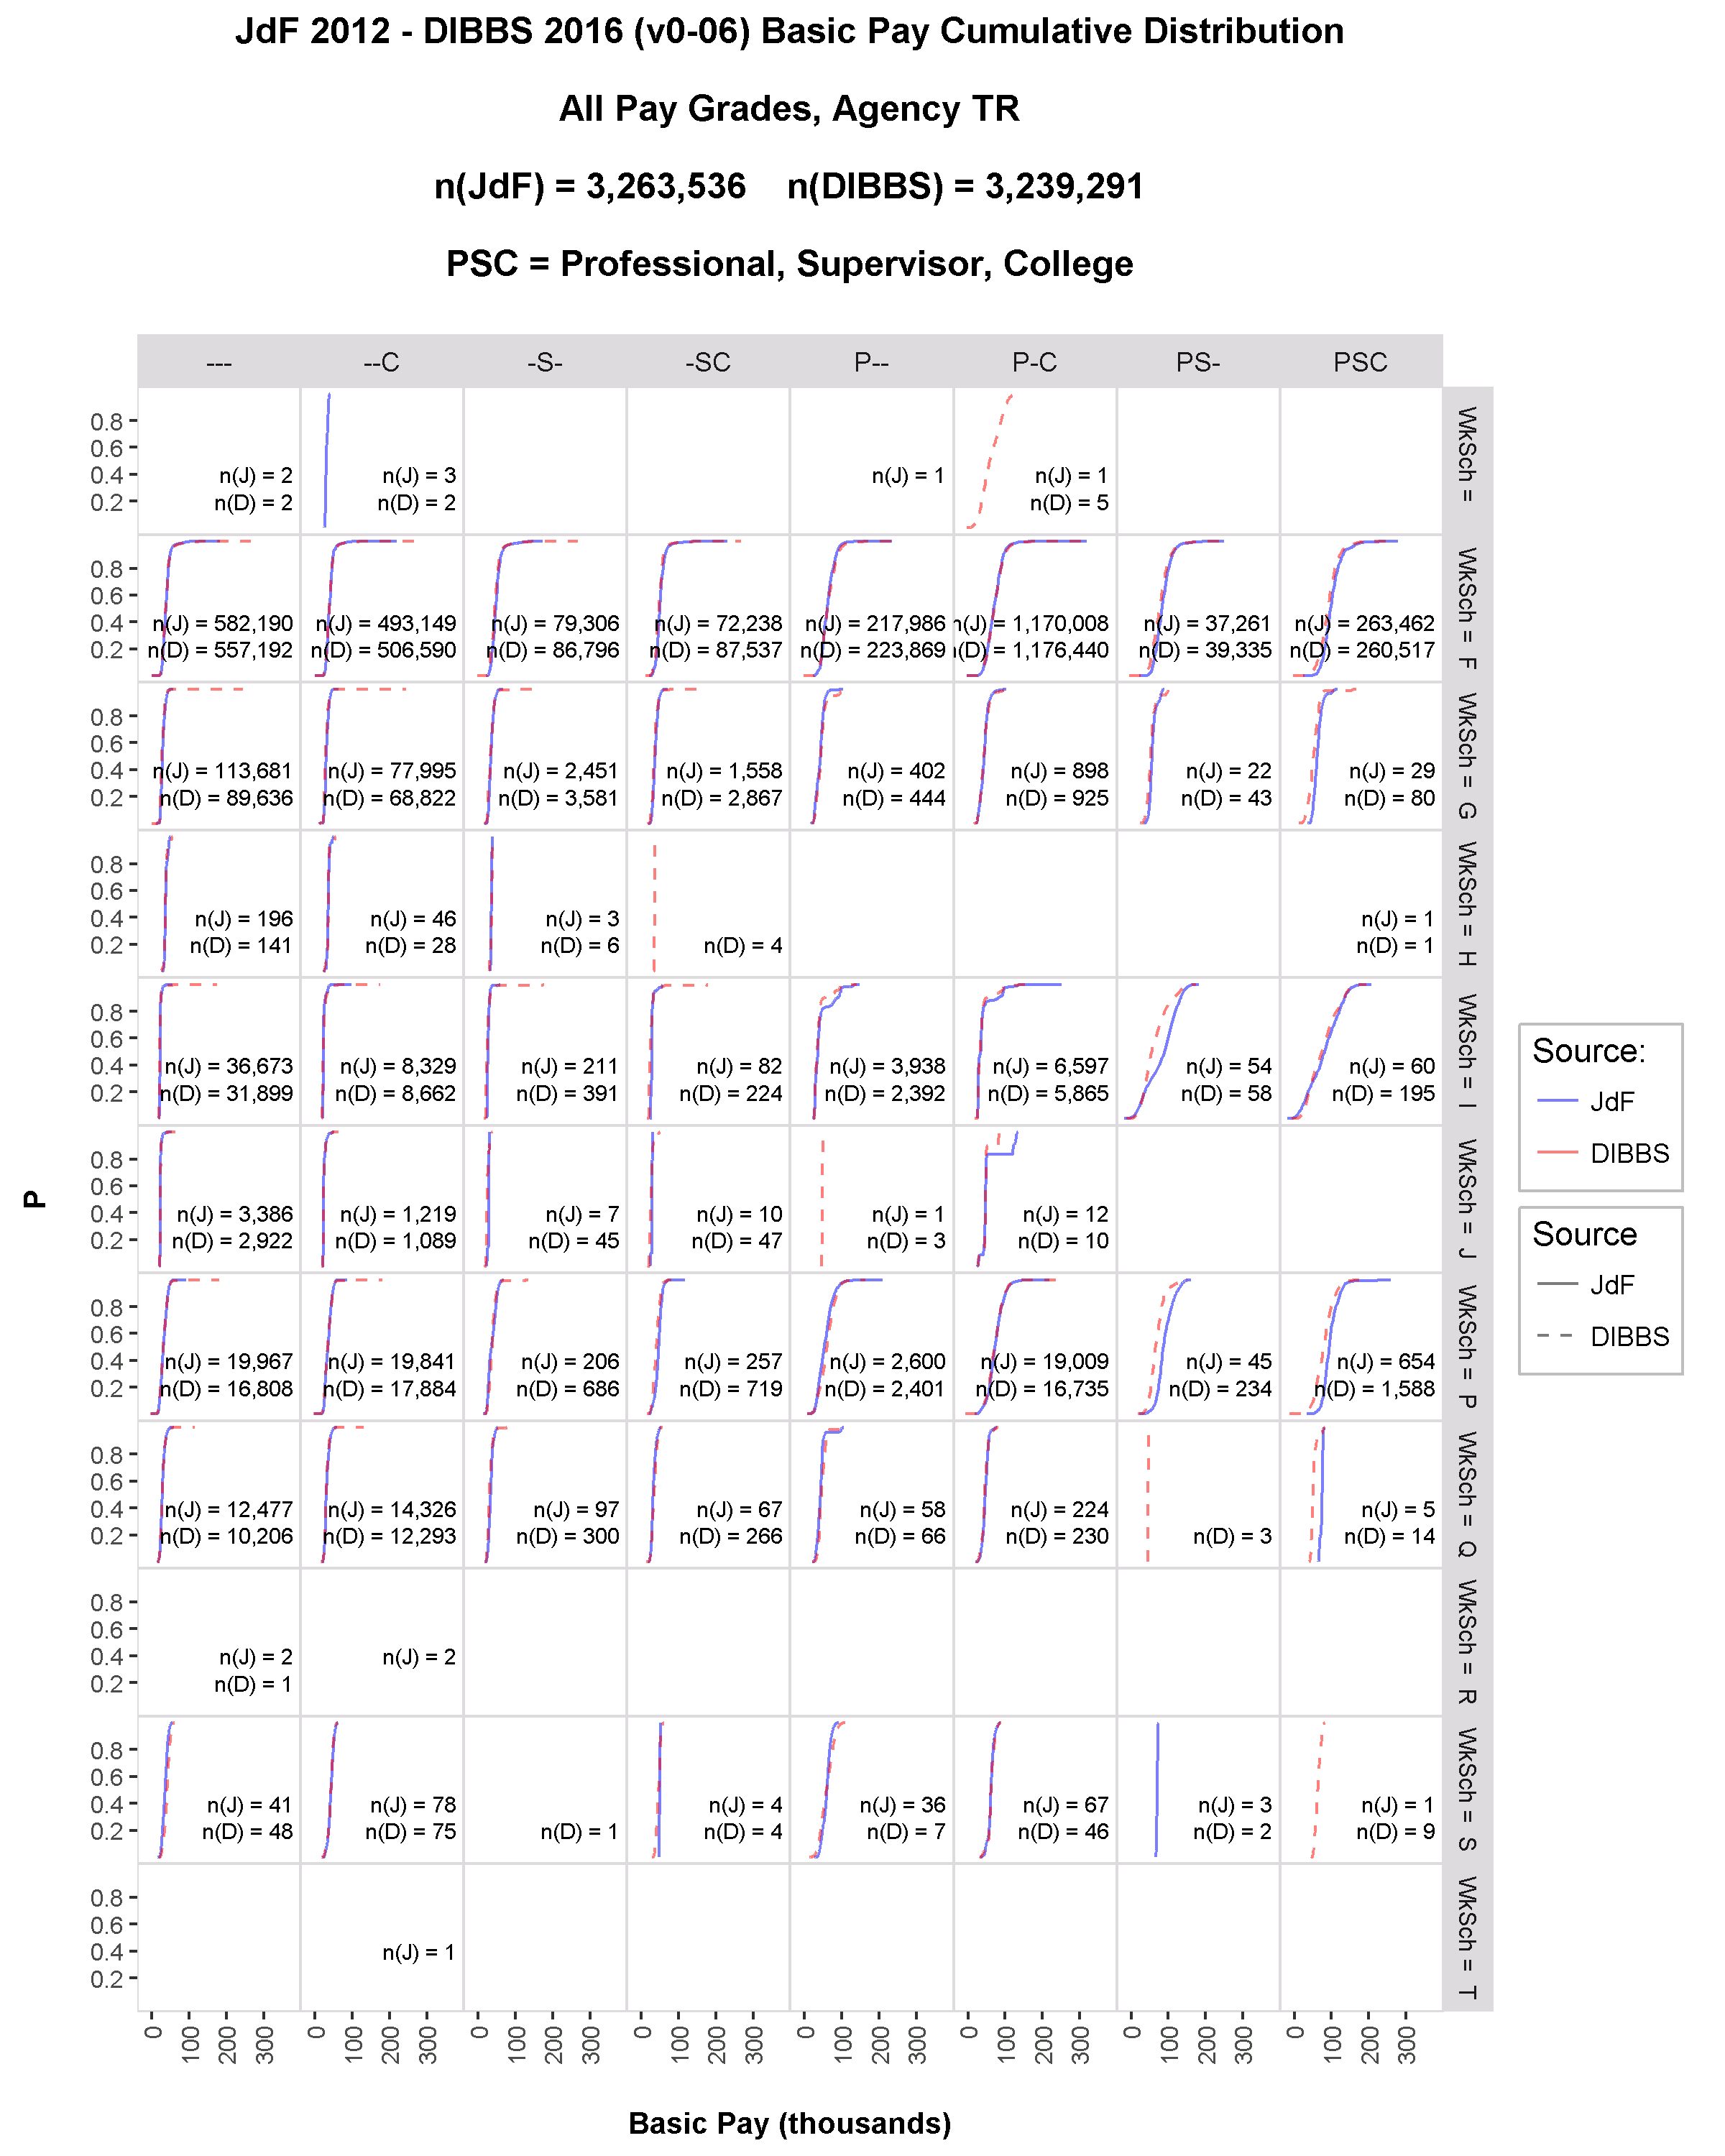
\includegraphics[width=6.5in, trim={0 0 1in 1.5in}, clip]{JdFDIBBSBasicPayCDFTR.png}
    \caption{Basic pay distribution by joint professional, supervisory status, college education, and work schedule  categories.  Department of Treasury (TR).  Dashed line for synthetic data, solid line for authentic.}
    \label{figure:JdFDIBBSBasicPayCDFTR}
\end{figure}

\clearpage

\begin{figure}[h]
    \centering
    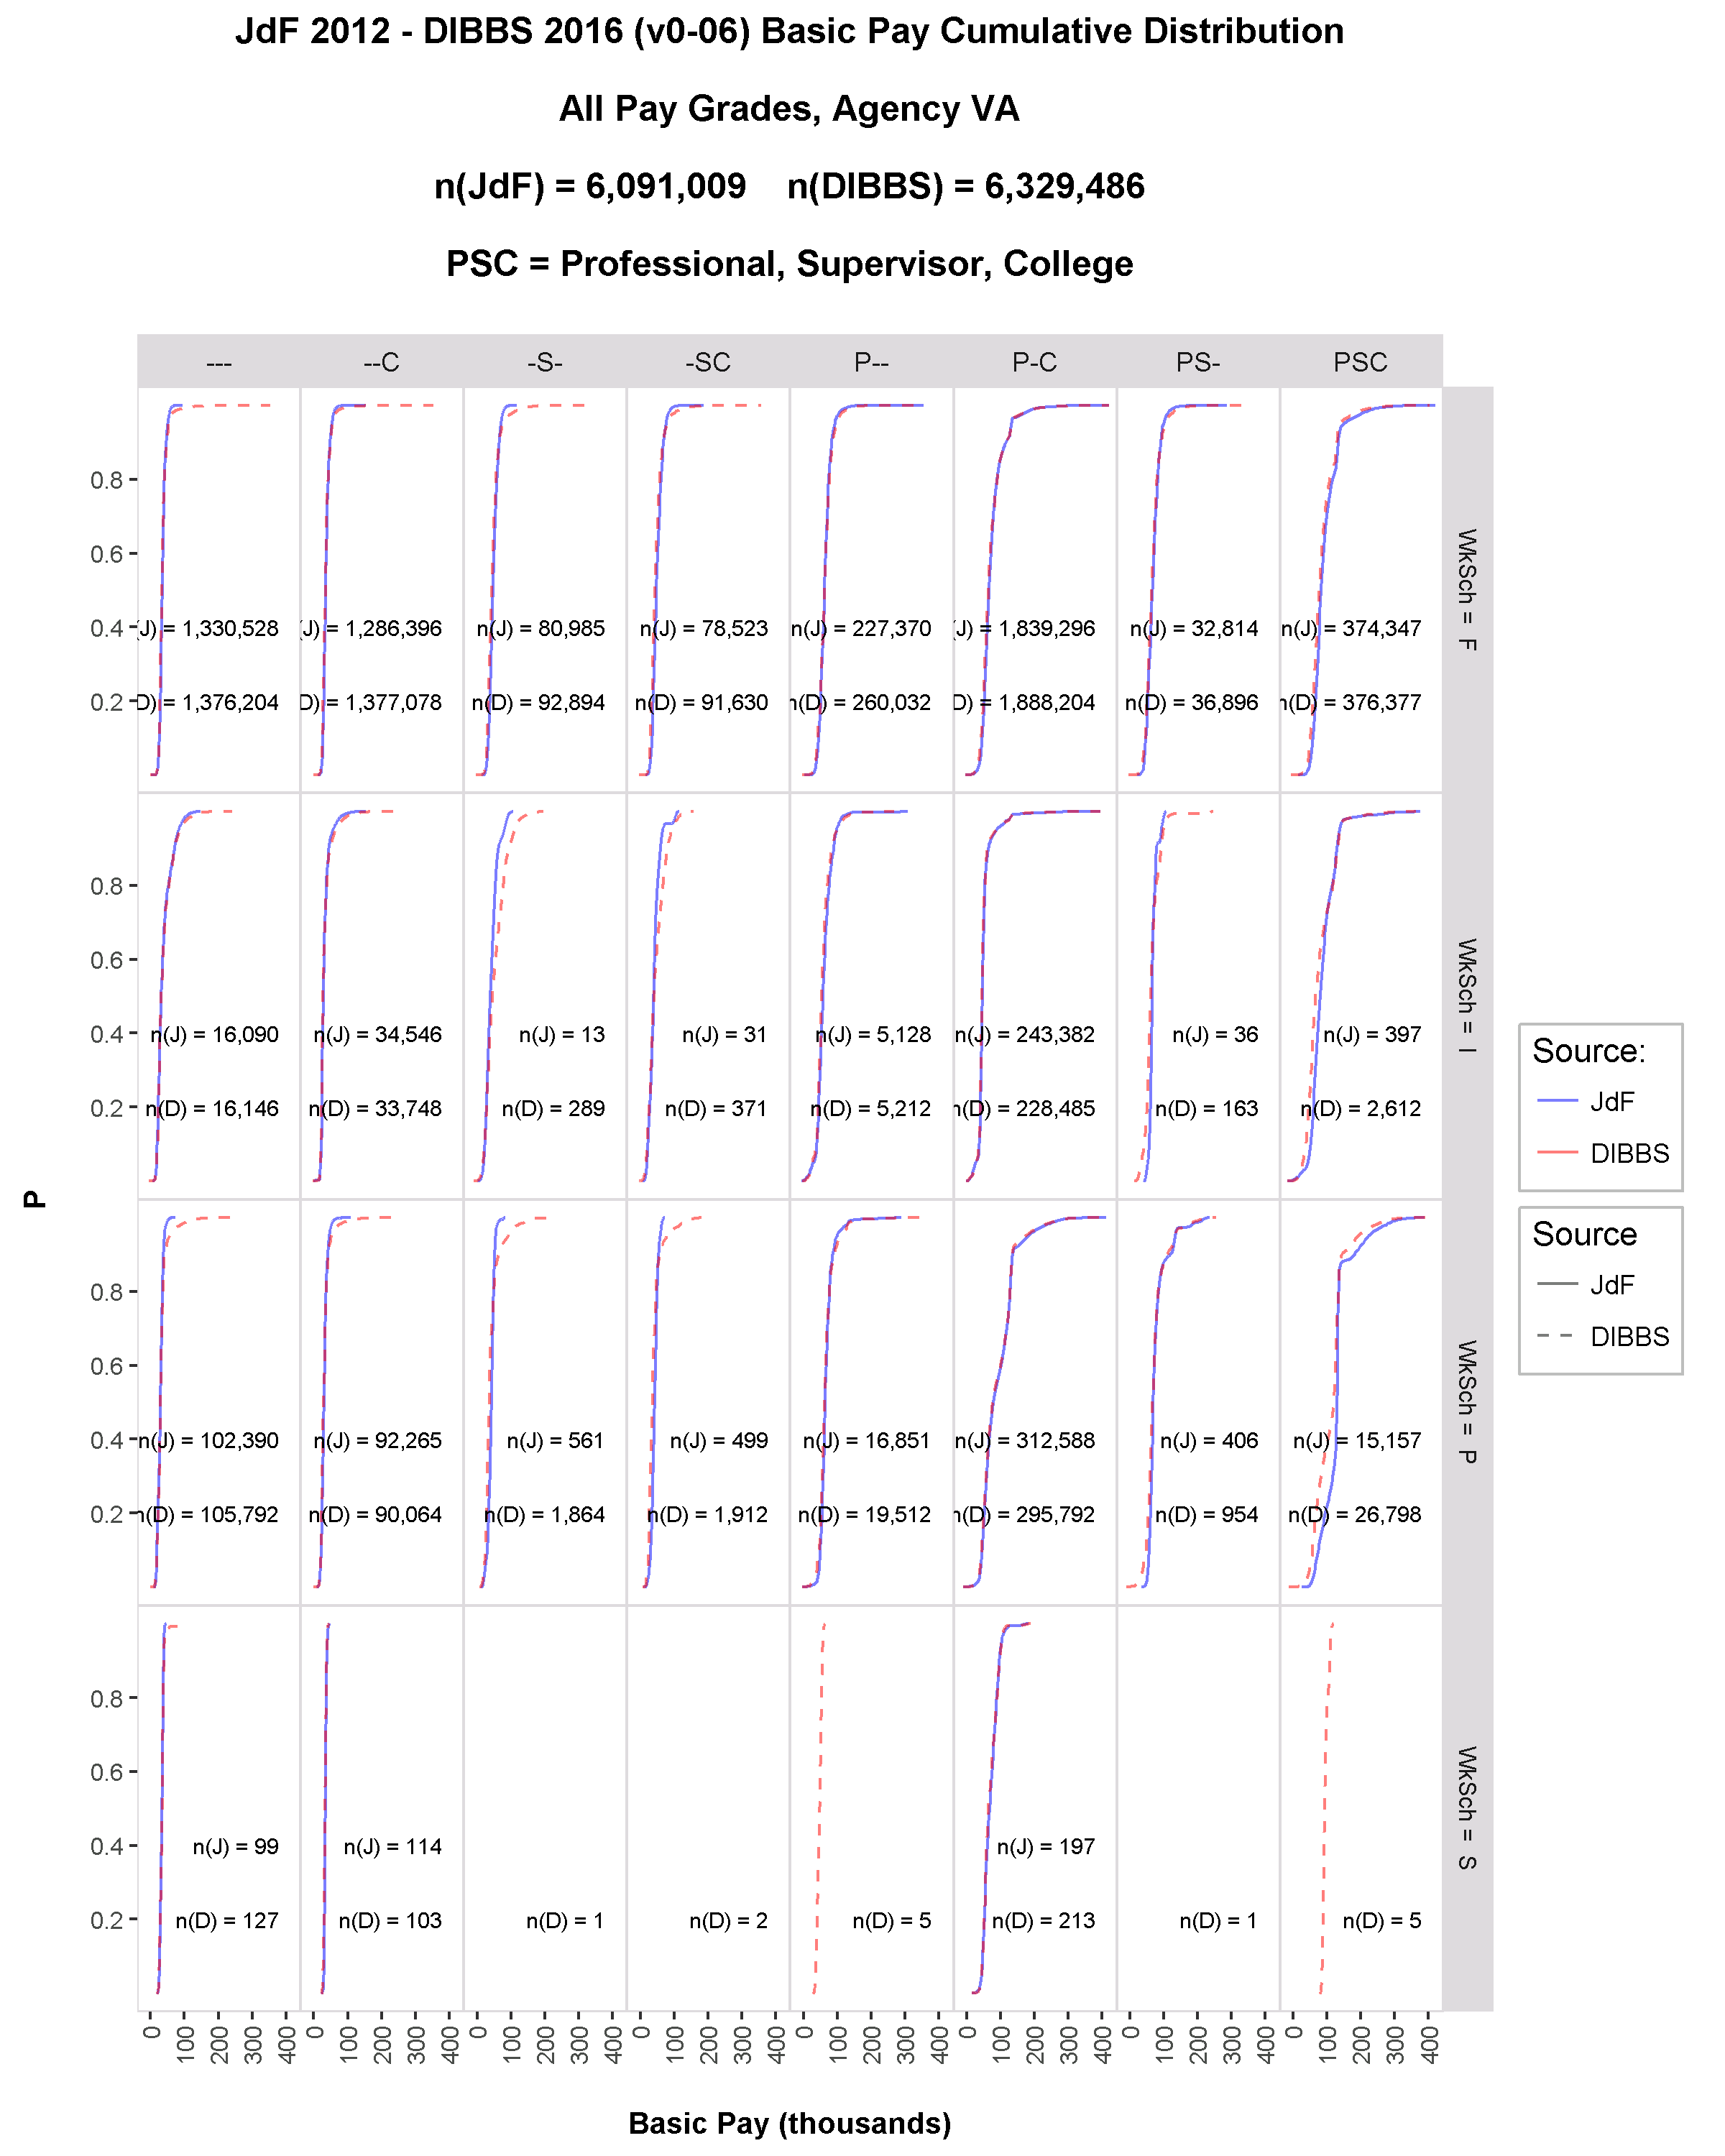
\includegraphics[width=6.5in, trim={0 0 1in 1.5in}, clip]{JdFDIBBSBasicPayCDFVA.png}
    \caption{Basic pay distribution by joint professional, supervisory status, college education, and work schedule  categories.  Department of Veterans Affairs (VA).  Dashed line for synthetic data, solid line for authentic.}
    \label{figure:JdFDIBBSBasicPayCDFVA}
\end{figure}

\clearpage

DISTRIBUTION OF BASIC PAY BY OCCUPATION AND SUPERVISORY STATUS\\

803 distinct occupations are represented in the data supplied by OPM.  To verify distribution of basic pay by occupation and supervisory status in the synthetic data, box plots consisting of a pair of authentic/synthetic distributions for each occupation were constructed.  Figures \ref{figure:JdFDIBBSBasicPaySupervisoryStatusOccupation1} through \ref{figure:JdFDIBBSBasicPaySupervisoryStatusOccupation3} show box plots for the first 120 occupations in order of occupation code.  Trade, or blue collar, occupations begin at code 2500.  Figures \ref{figure:JdFDIBBSBasicPaySupervisoryStatusOccupation4} and \ref{figure:JdFDIBBSBasicPaySupervisoryStatusOccupation5} show the distributions of the first 80 of these occupations.  Remaining occupations exhibit patterns similar to those presented.\\

Observation:  Median pay and inter-quartile ranges appear consistent between data sets.  Upper tails of distributions of in the synthetic data generally appear greater than corresponding authentic distributions, particulary for trade occupations.  Note that, of the 318 trade occupations represented in the authentic data, 190 have proportion female observations less than 0.05.  Given disparity in federal employee pay by gender \citep{BoltondeFigGenderPayGap2017} and a requirement, for protection of privacy, of a degree of modification of gender and occupation in synthetic observations, differences in pay extremes may be expected.\\

\begin{figure}[h]
    \centering
    \begin{subfigure}{1\textwidth}
        \centering
        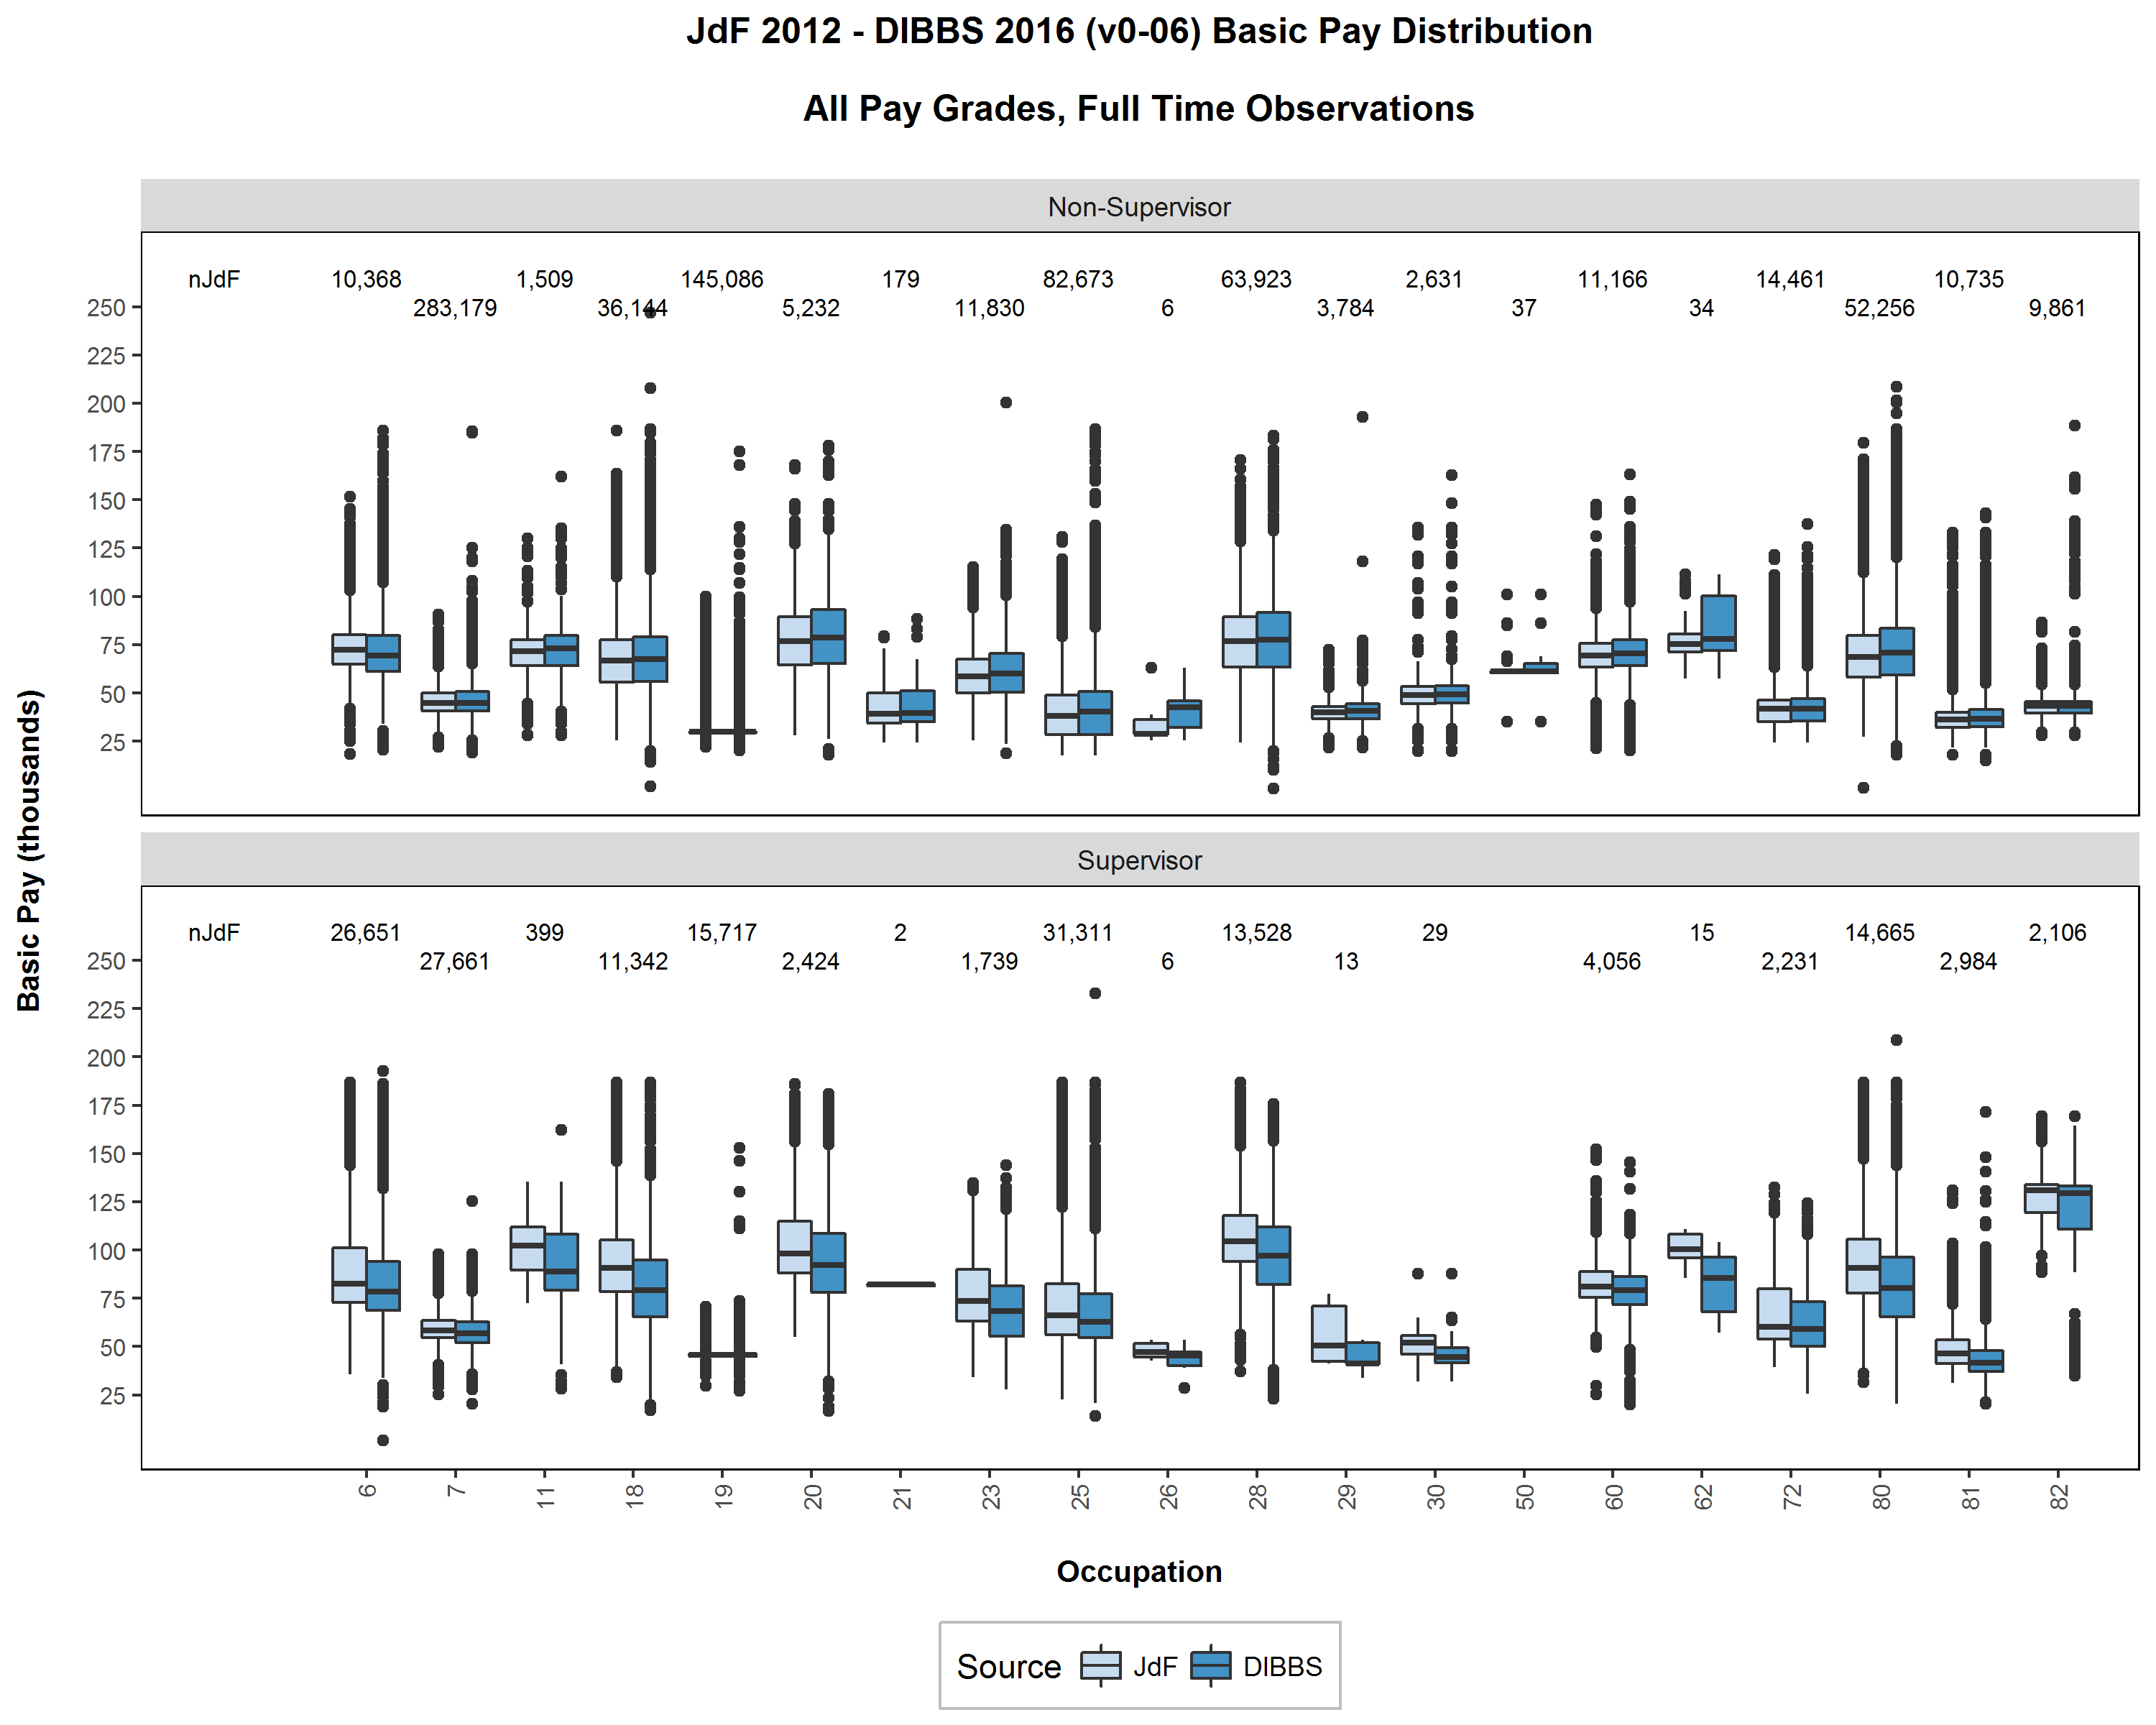
\includegraphics[width=6in, trim={0 1in 0 0.75in}, clip]{JdFDIBBSBasicPaySupervisoryStatusOccupation1.png}
        \caption{Occupations 0006 through 0082}
        \vspace{10pt}
    \end{subfigure}
    \begin{subfigure}{1\textwidth}
        \centering
        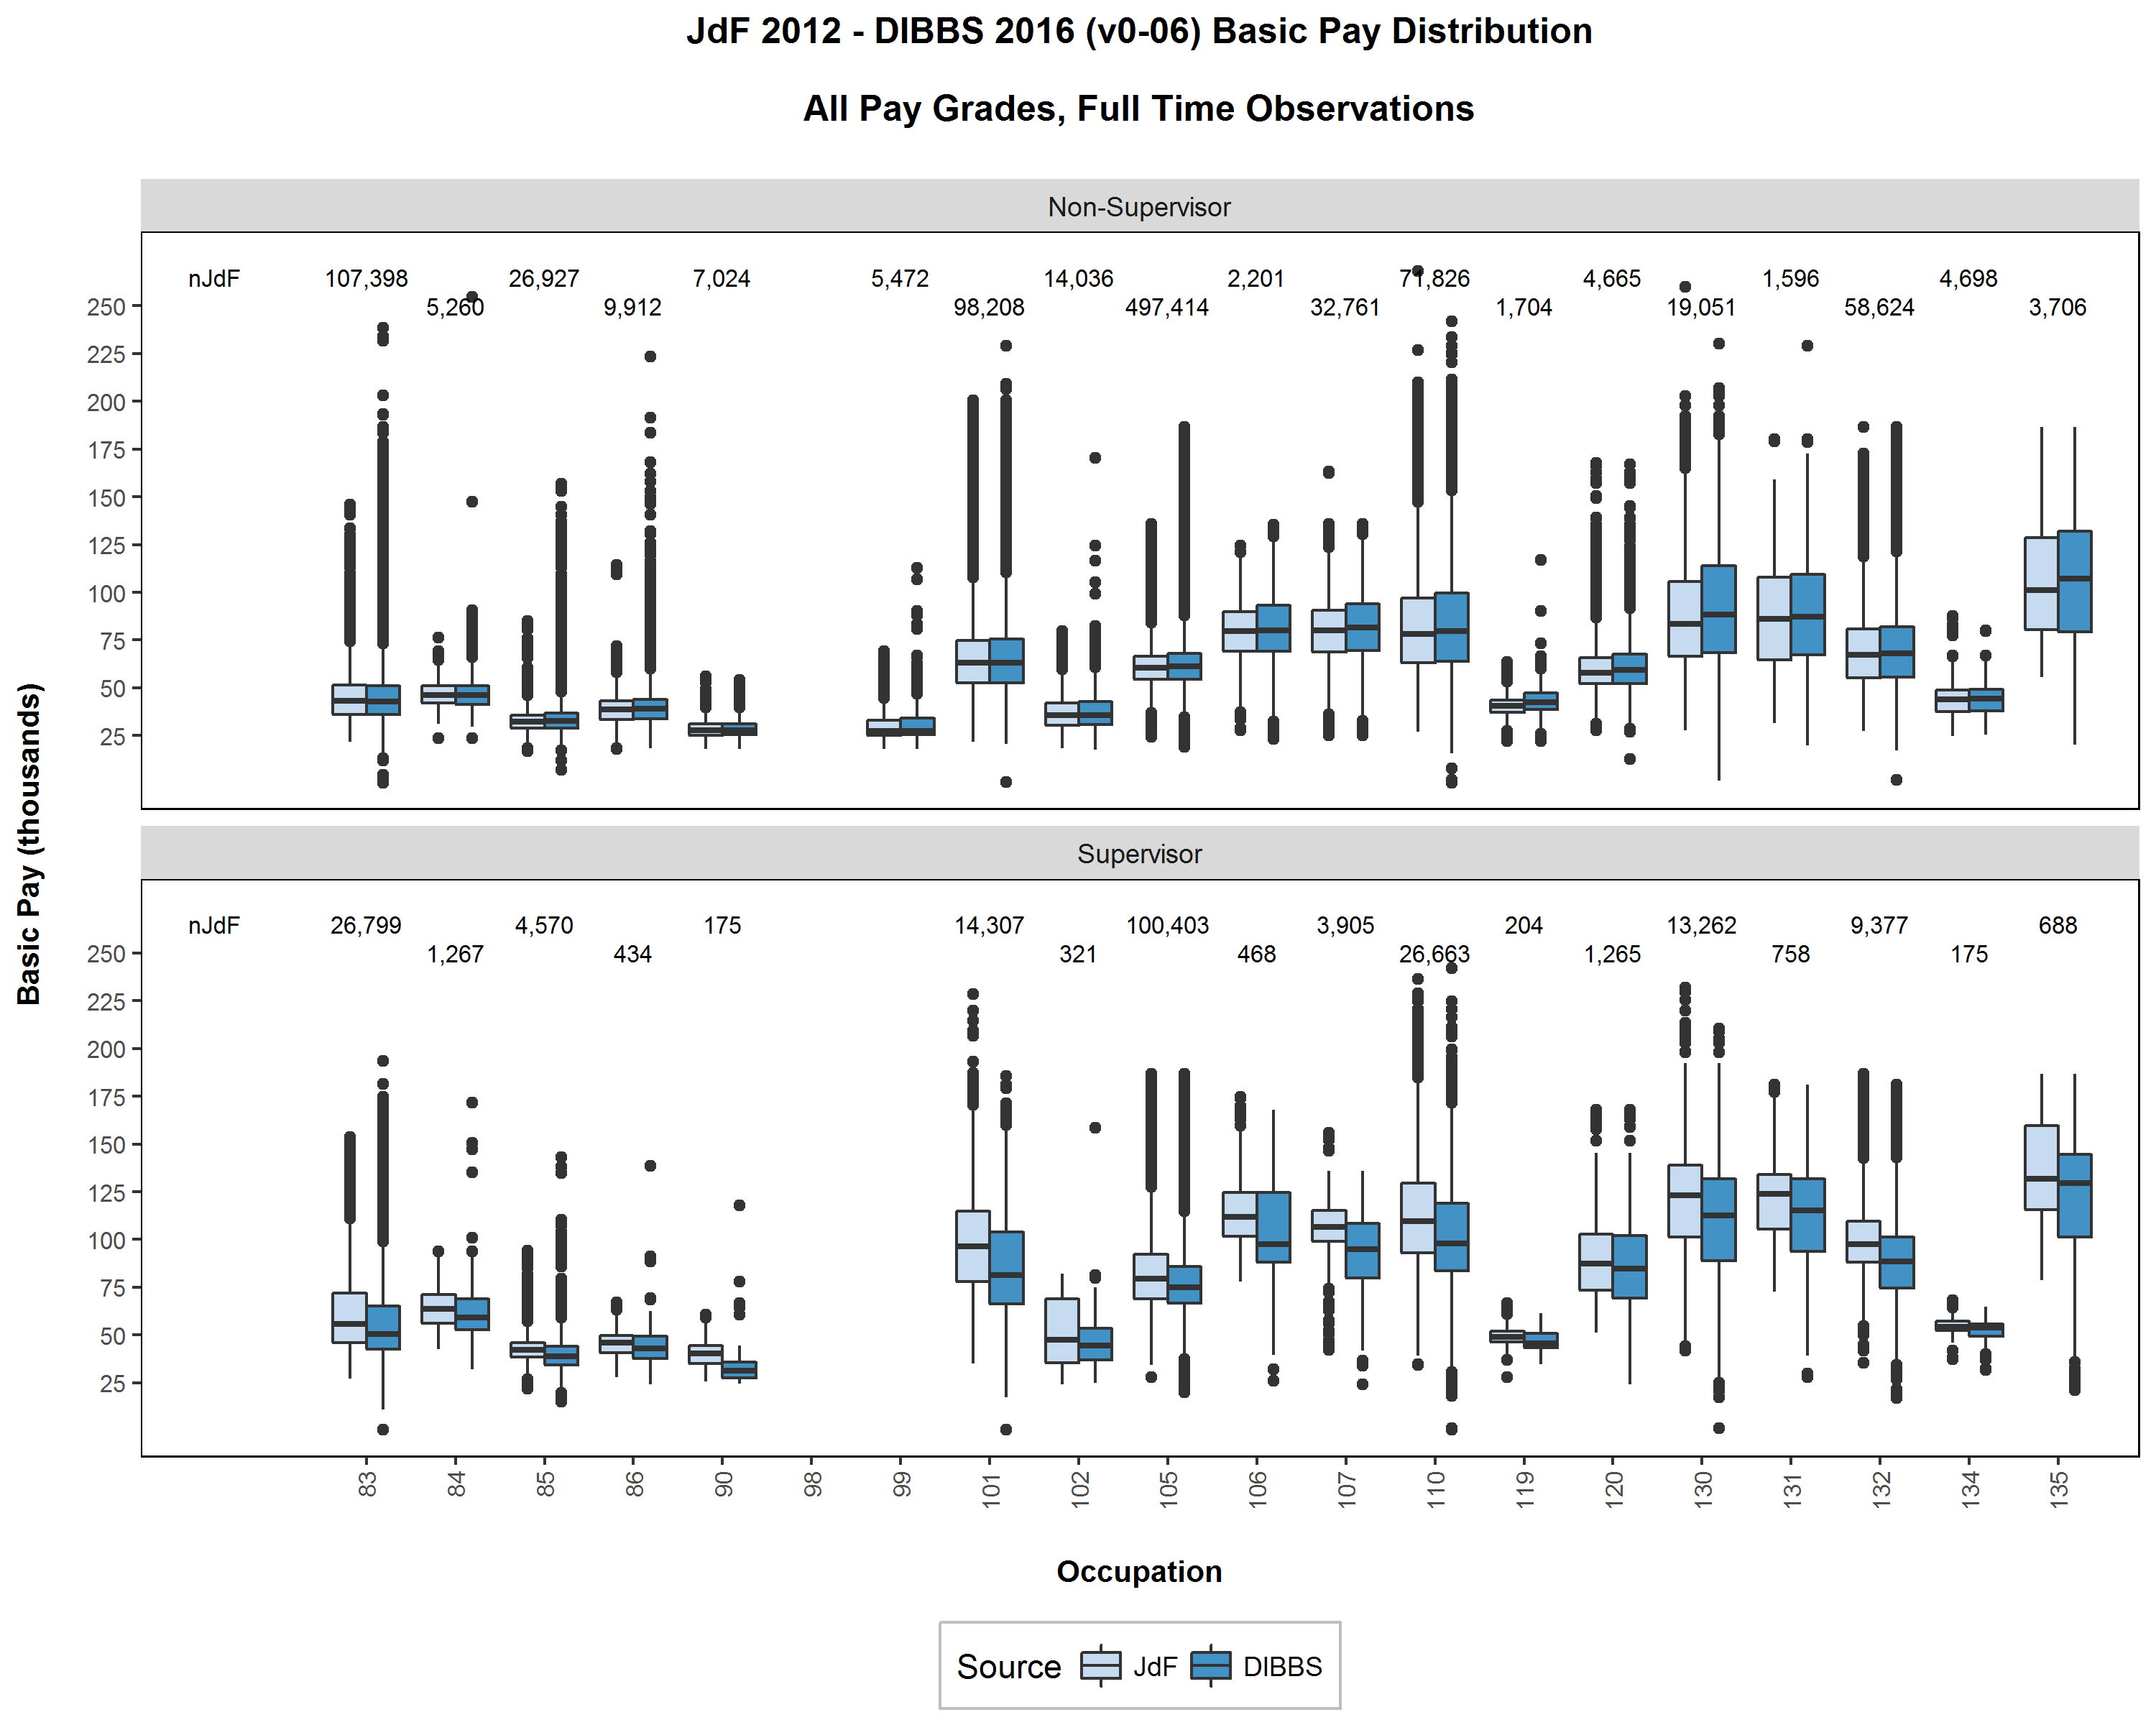
\includegraphics[width=6in, trim={0 1in 0 0.75in}, clip]{JdFDIBBSBasicPaySupervisoryStatusOccupation21.png}
        \caption{Occupations 0083 through 0135}
        \vspace{10pt}
    \end{subfigure}
    \caption{Basic pay distribution by occupation and supervisor status.  All agencies combined.  Authentic boxes on left, synthetic on right.}
    \label{figure:JdFDIBBSBasicPaySupervisoryStatusOccupation1}
\end{figure}

\clearpage

\begin{figure}[h]
    \centering
    \begin{subfigure}{1\textwidth}
        \centering
        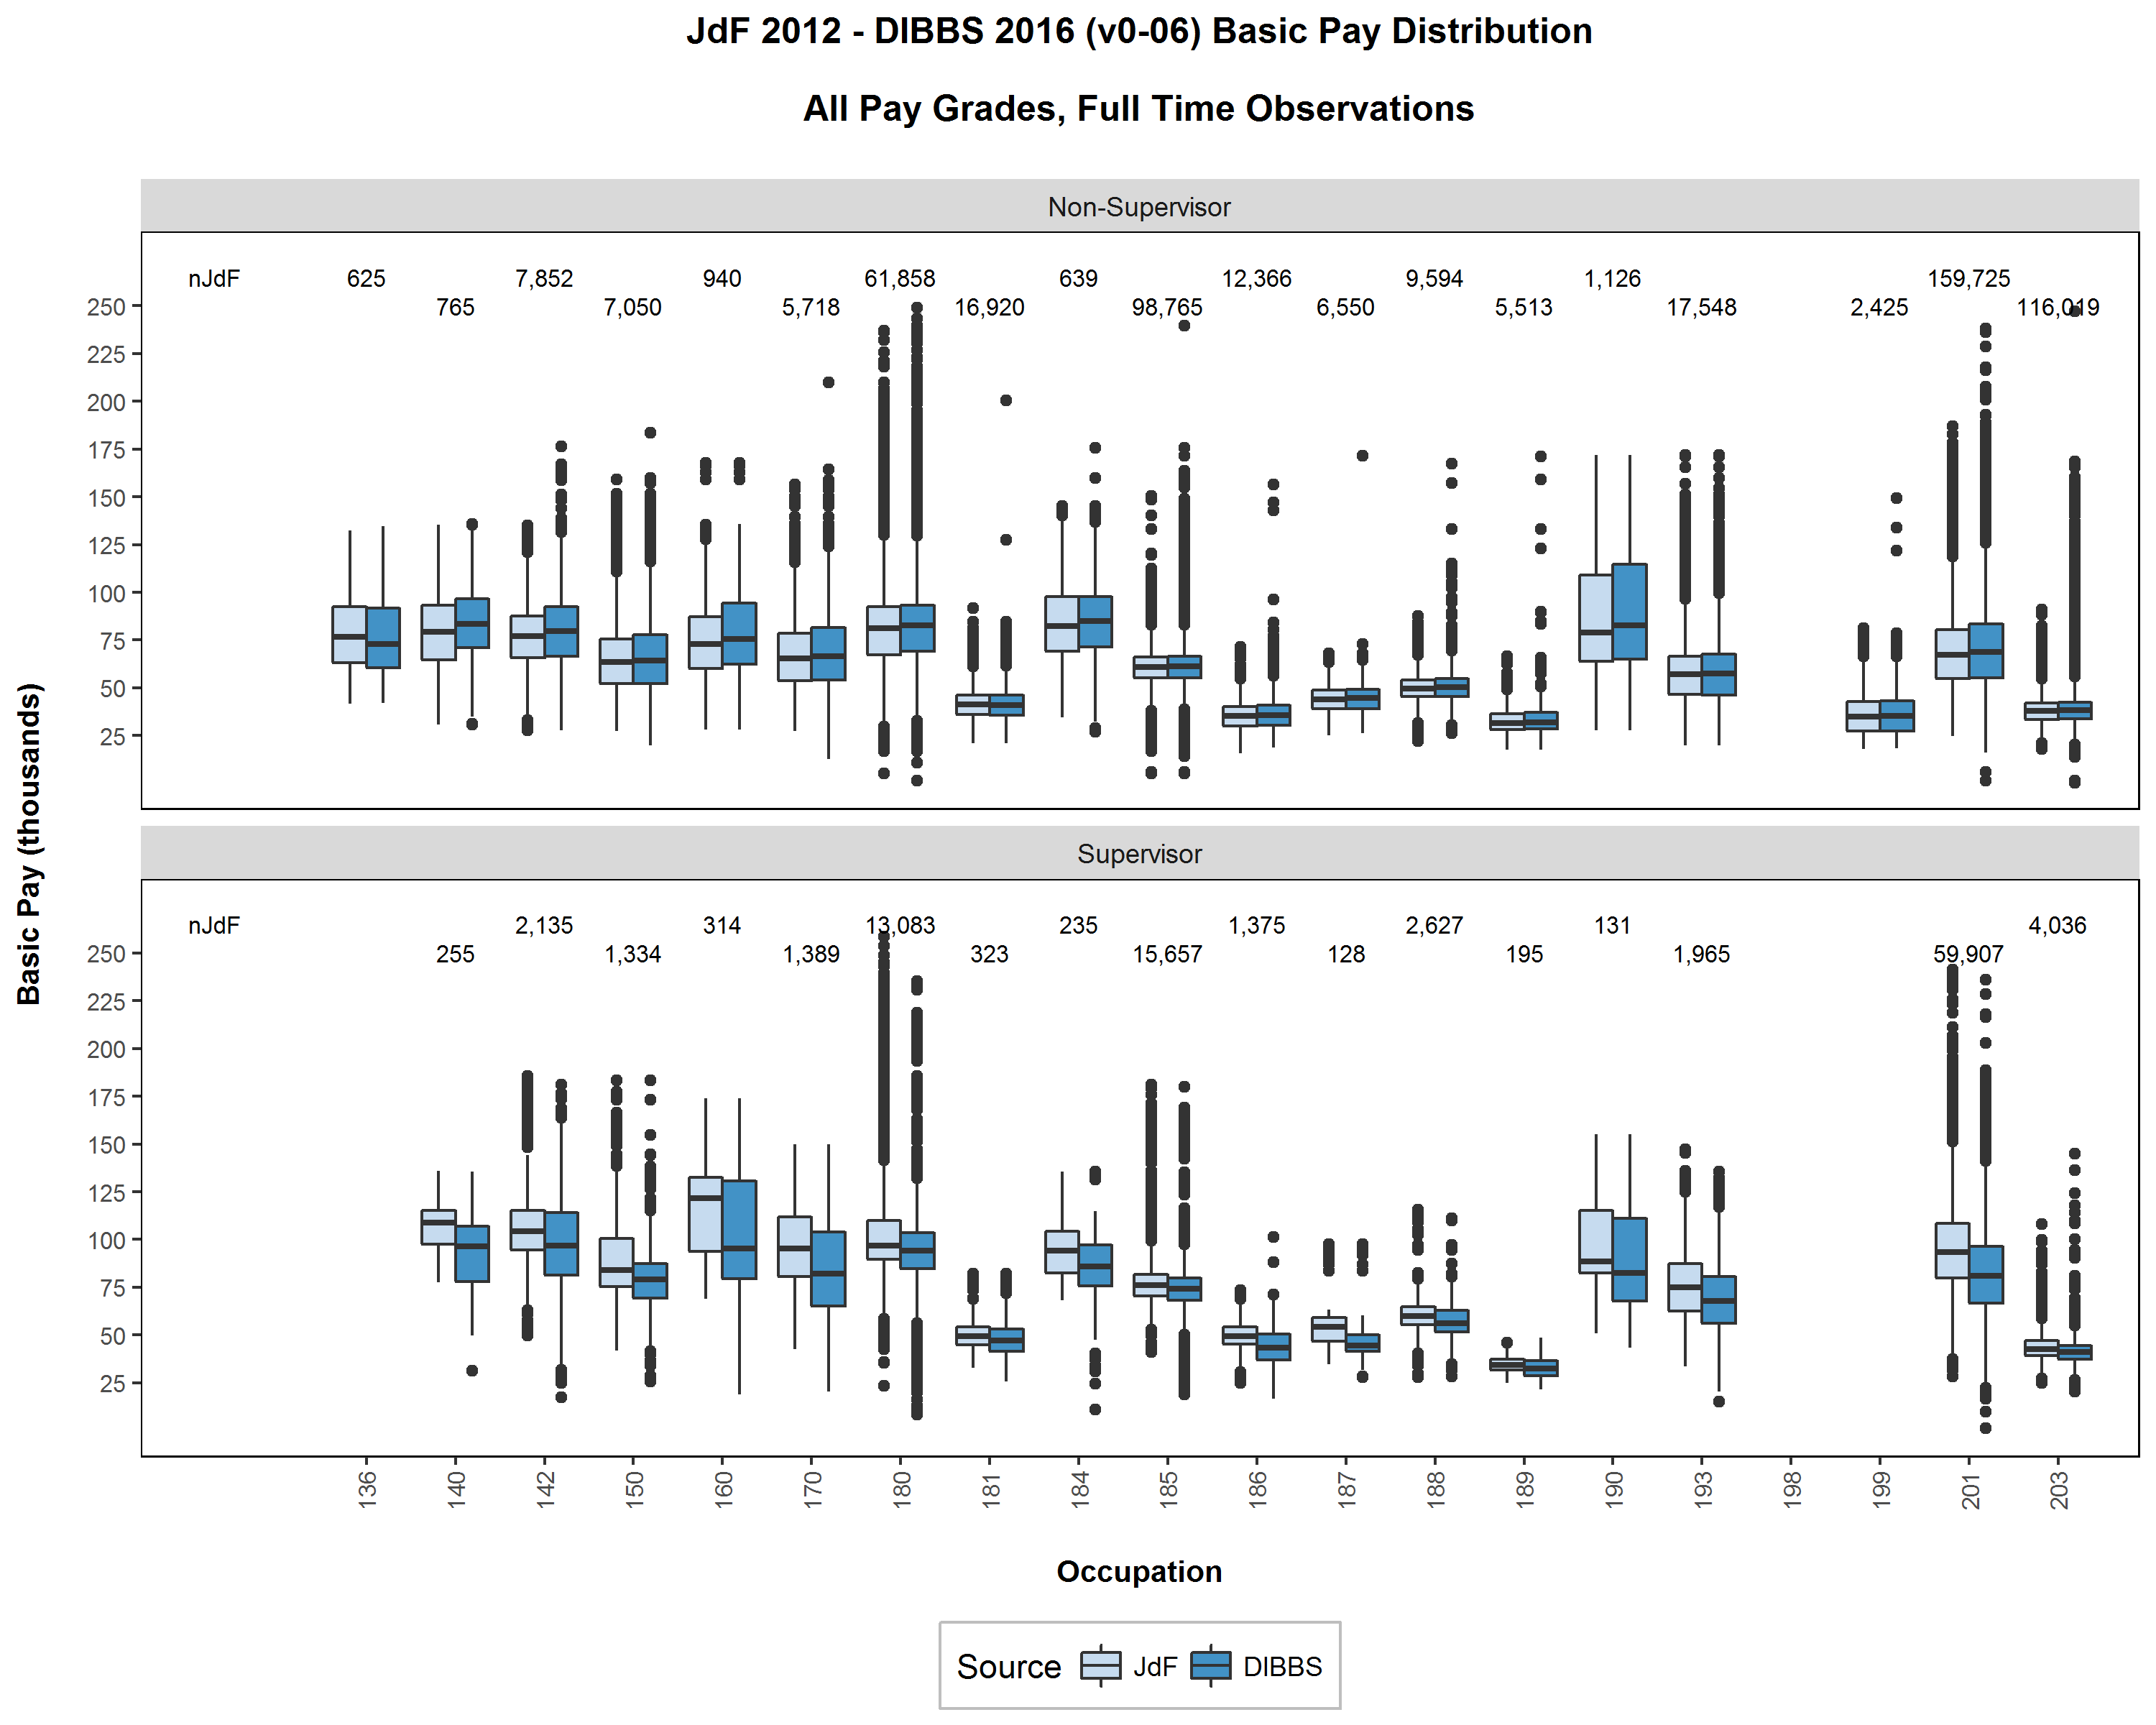
\includegraphics[width=6in, trim={0 1in 0 0.75in}, clip]{JdFDIBBSBasicPaySupervisoryStatusOccupation41.png}
        \caption{Occupations 0136 through 0203}
        \vspace{10pt}
    \end{subfigure}
    \begin{subfigure}{1\textwidth}
        \centering
        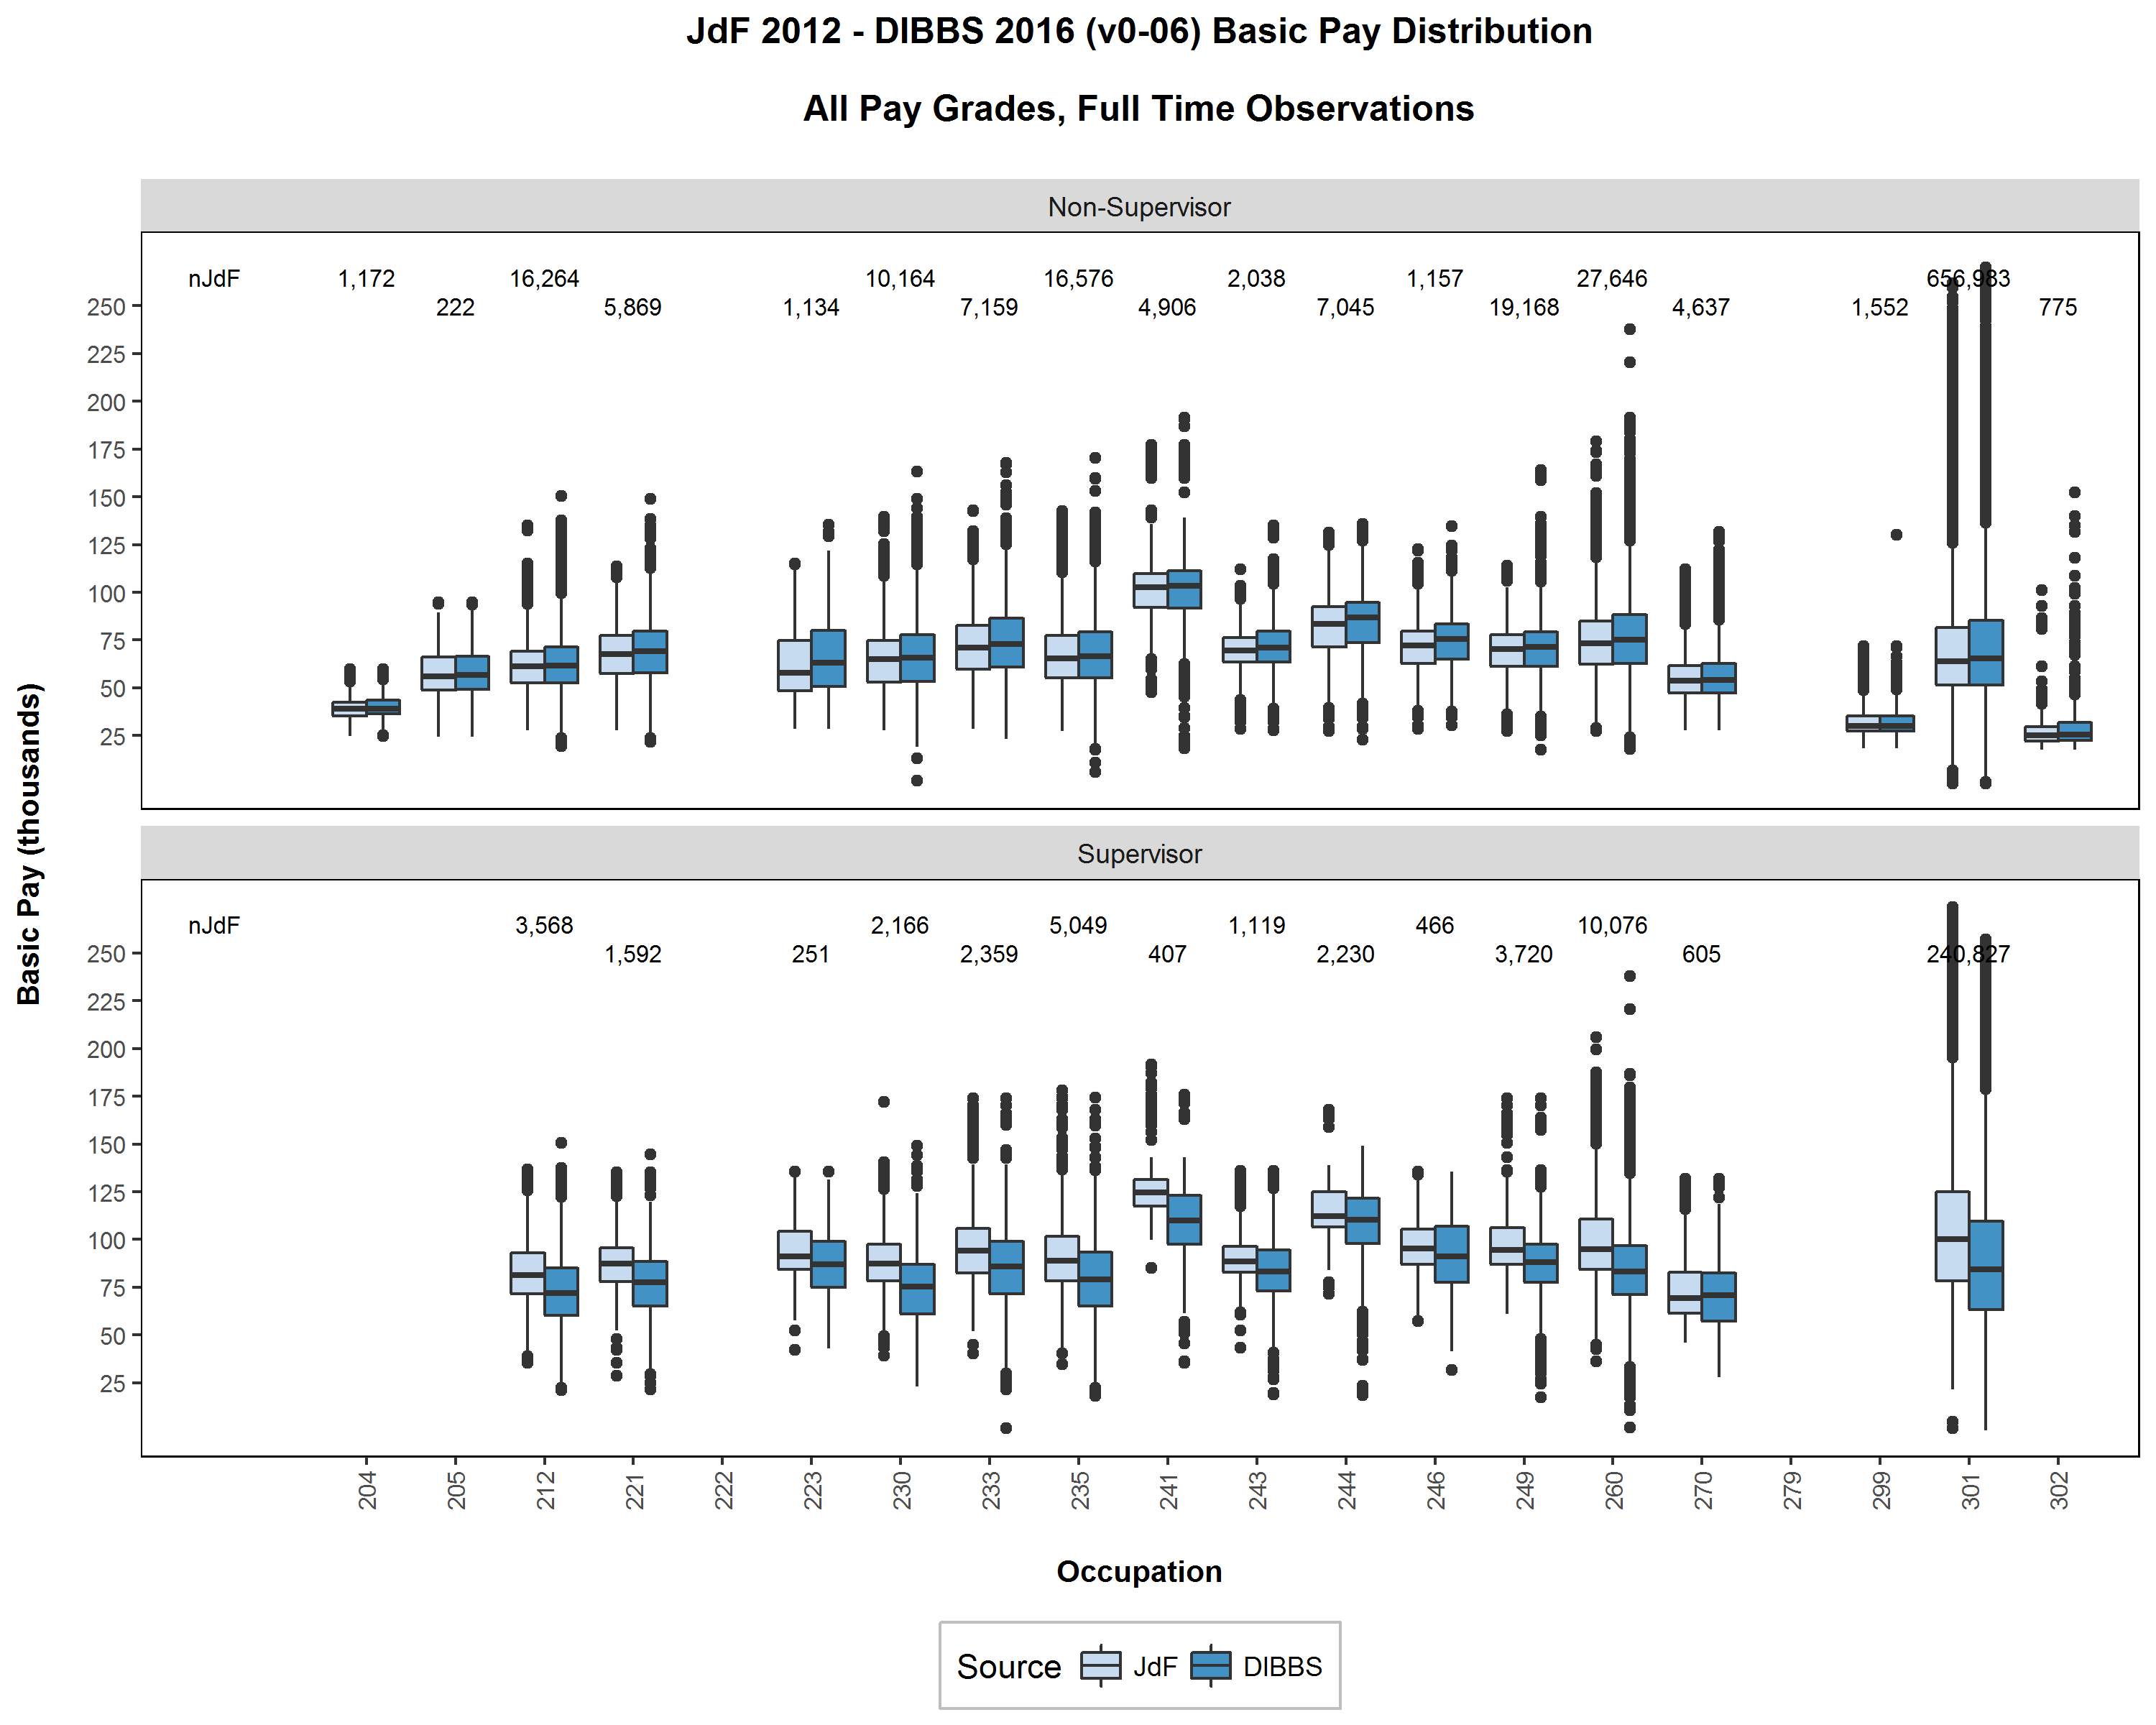
\includegraphics[width=6in, trim={0 1in 0 0.75in}, clip]{JdFDIBBSBasicPaySupervisoryStatusOccupation61.png}
        \caption{Occupations 0204 through 0302}
        \vspace{10pt}
    \end{subfigure}
    \caption{Basic pay distribution by occupation and supervisor status.  All agencies combined.  Authentic boxes on left, synthetic on right.}
    \label{figure:JdFDIBBSBasicPaySupervisoryStatusOccupation2}
\end{figure}

\clearpage

\begin{figure}[h]
    \centering
    \begin{subfigure}{1\textwidth}
        \centering
        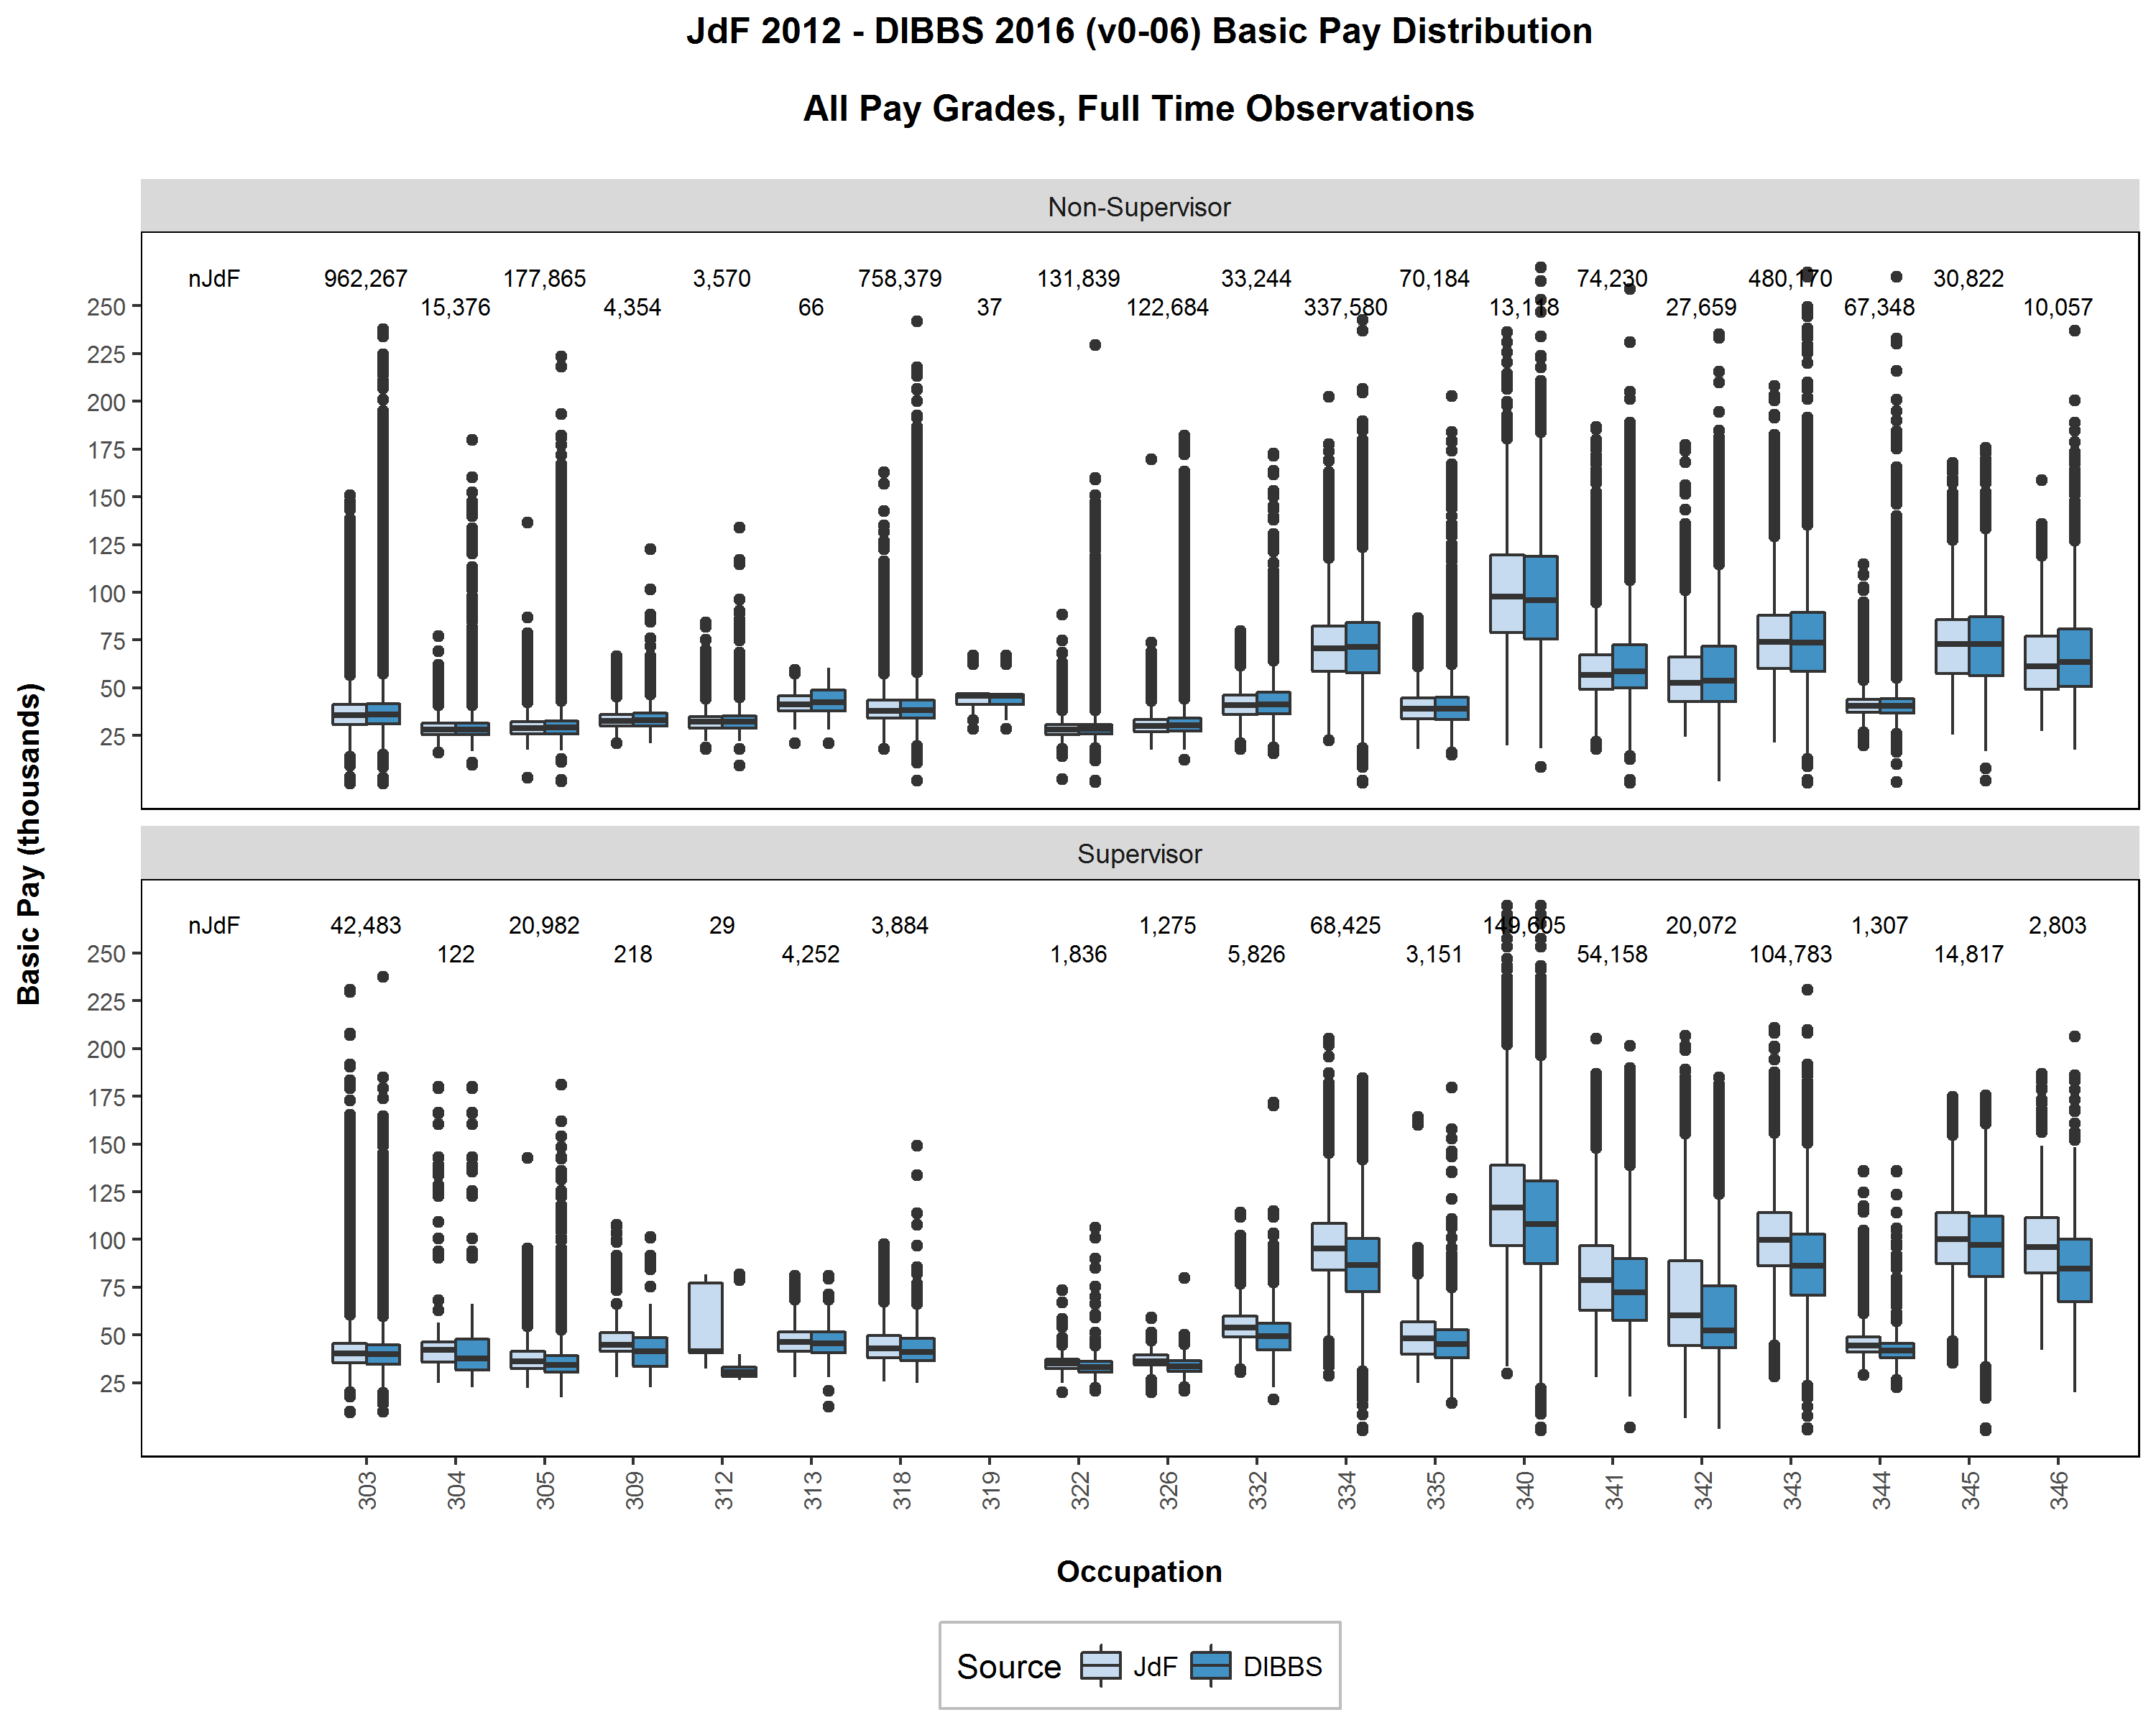
\includegraphics[width=6in, trim={0 1in 0 0.75in}, clip]{JdFDIBBSBasicPaySupervisoryStatusOccupation81.png}
        \caption{Occupations 0303 through 0346}
        \vspace{10pt}
    \end{subfigure}
    \begin{subfigure}{1\textwidth}
        \centering
        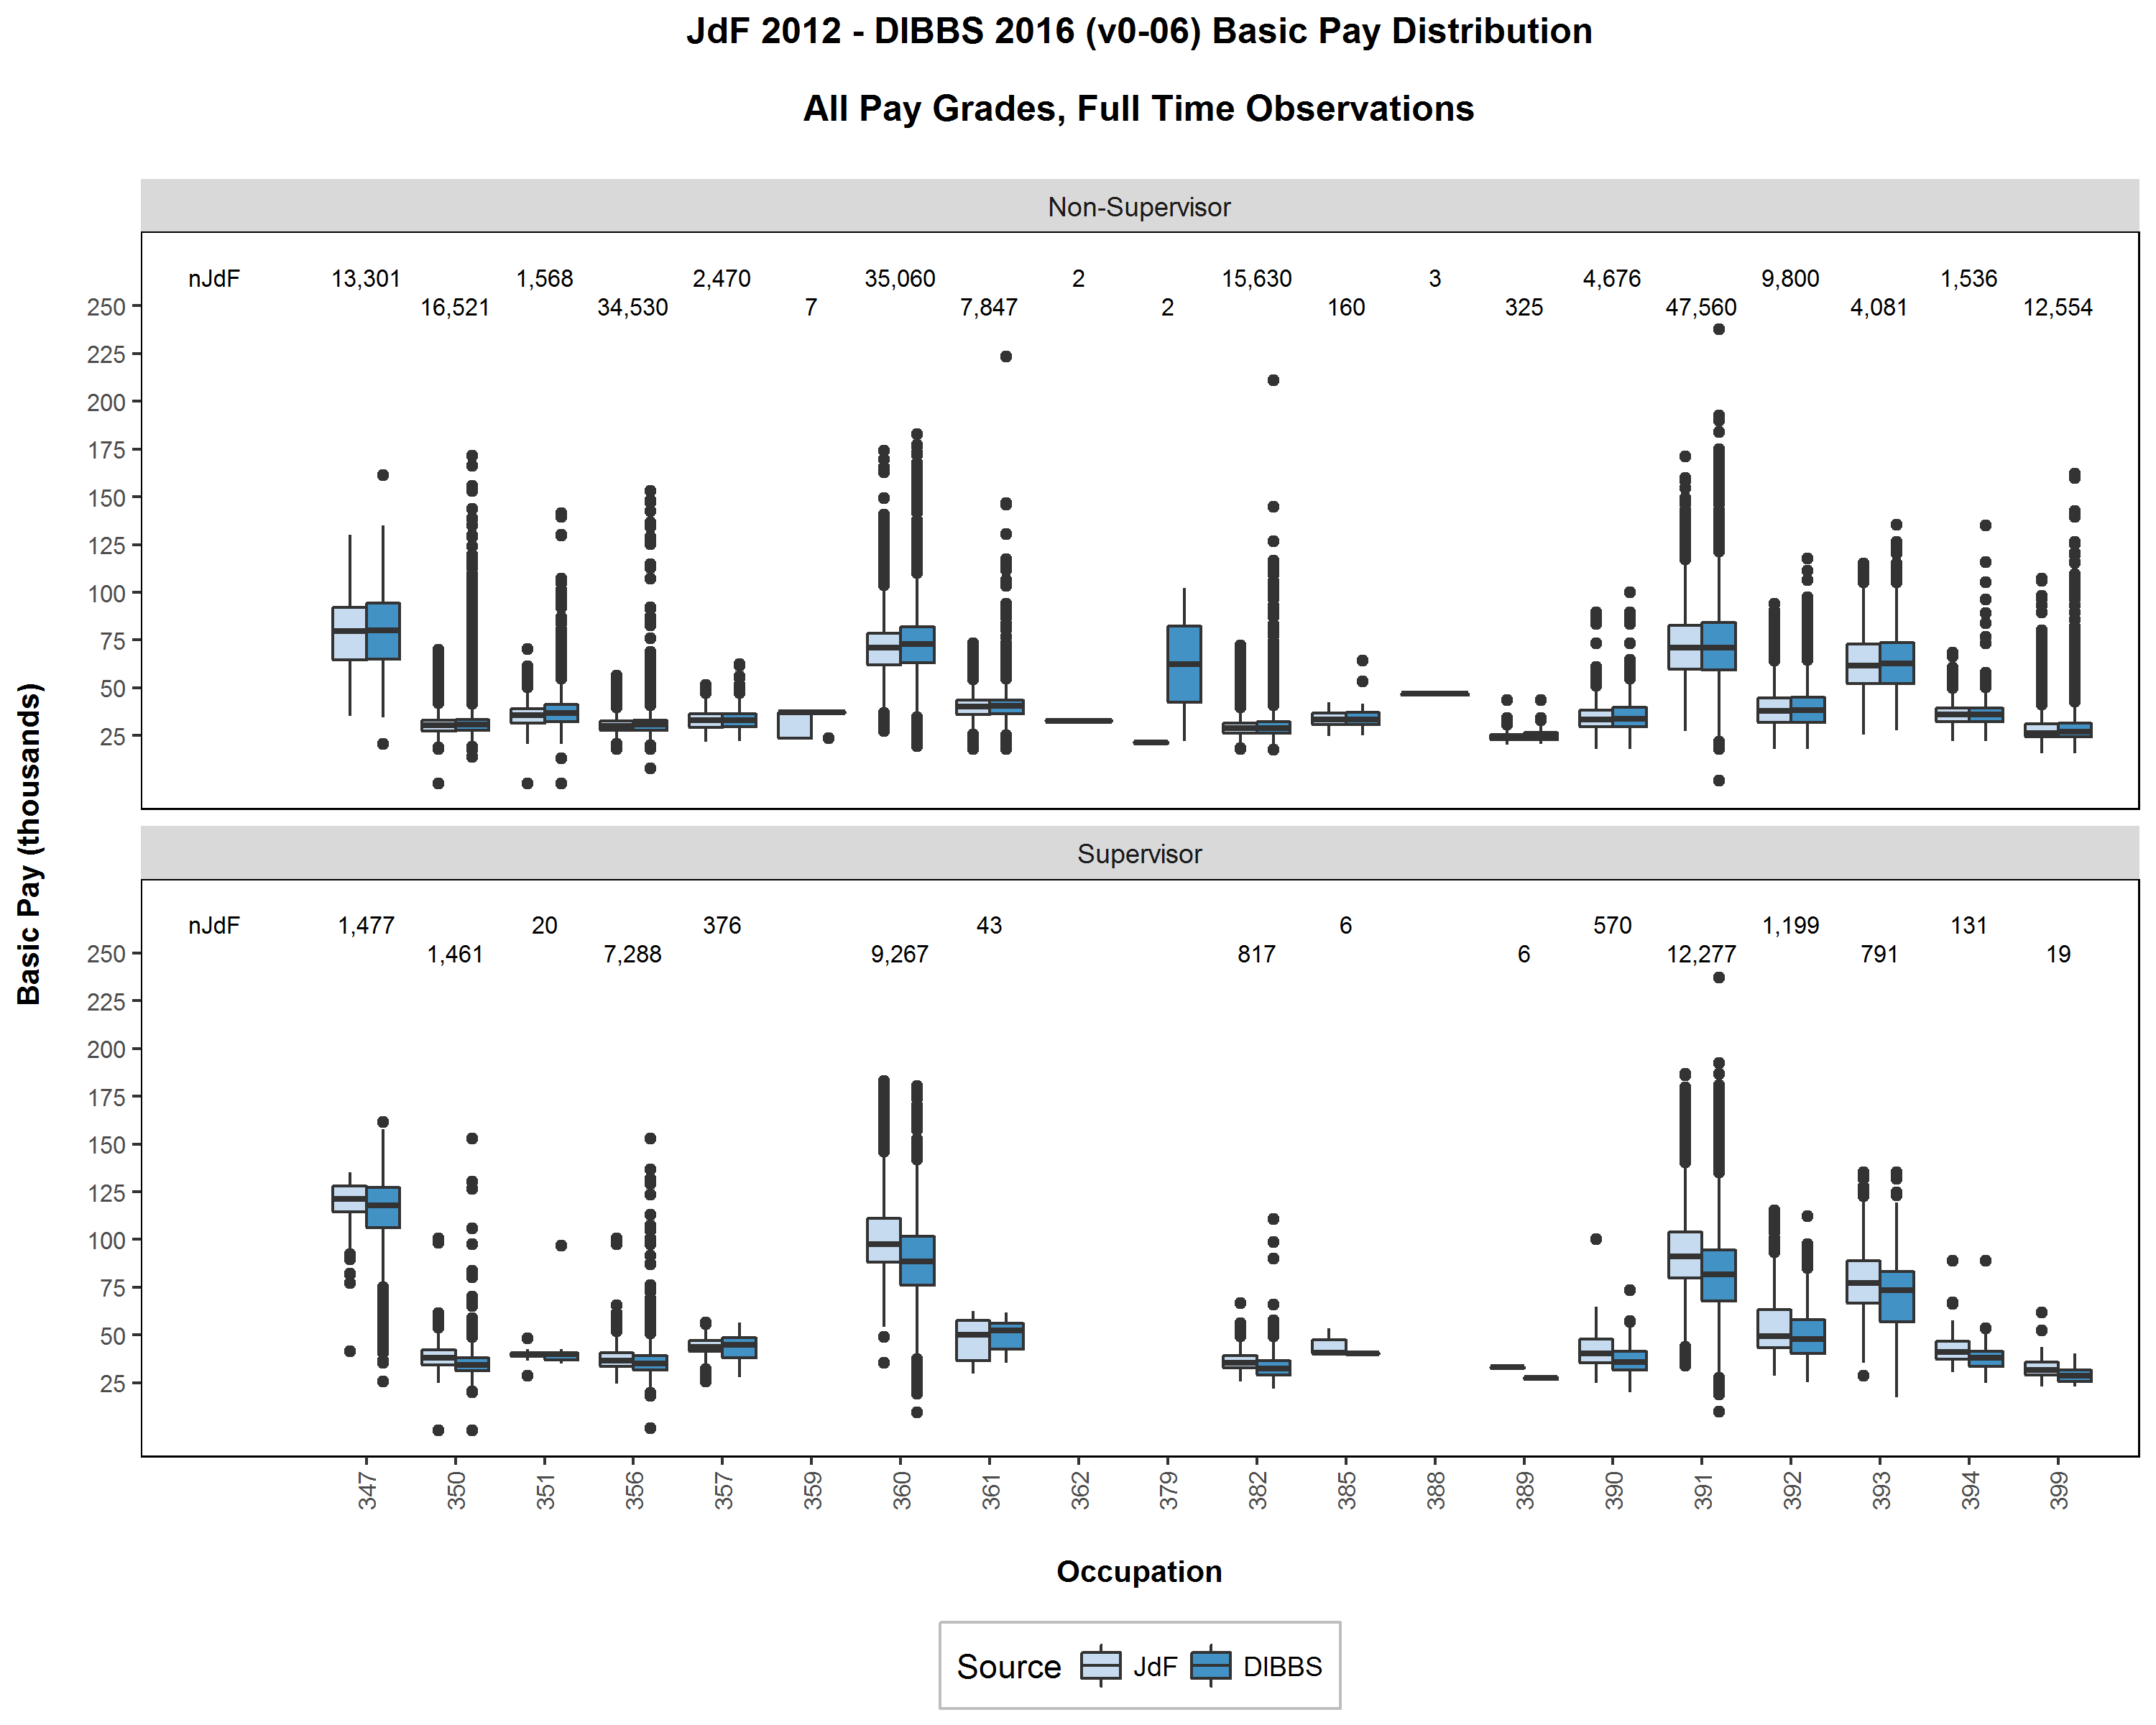
\includegraphics[width=6in, trim={0 1in 0 0.75in}, clip]{JdFDIBBSBasicPaySupervisoryStatusOccupation101.png}
        \caption{Occupations 0347 through 0399}
        \vspace{10pt}
    \end{subfigure}
    \caption{Basic pay distribution by occupation and supervisor status.  All agencies combined.  Authentic boxes on left, synthetic on right.}
    \label{figure:JdFDIBBSBasicPaySupervisoryStatusOccupation3}
\end{figure}

\begin{figure}[h]
    \centering
    \begin{subfigure}{1\textwidth}
        \centering
        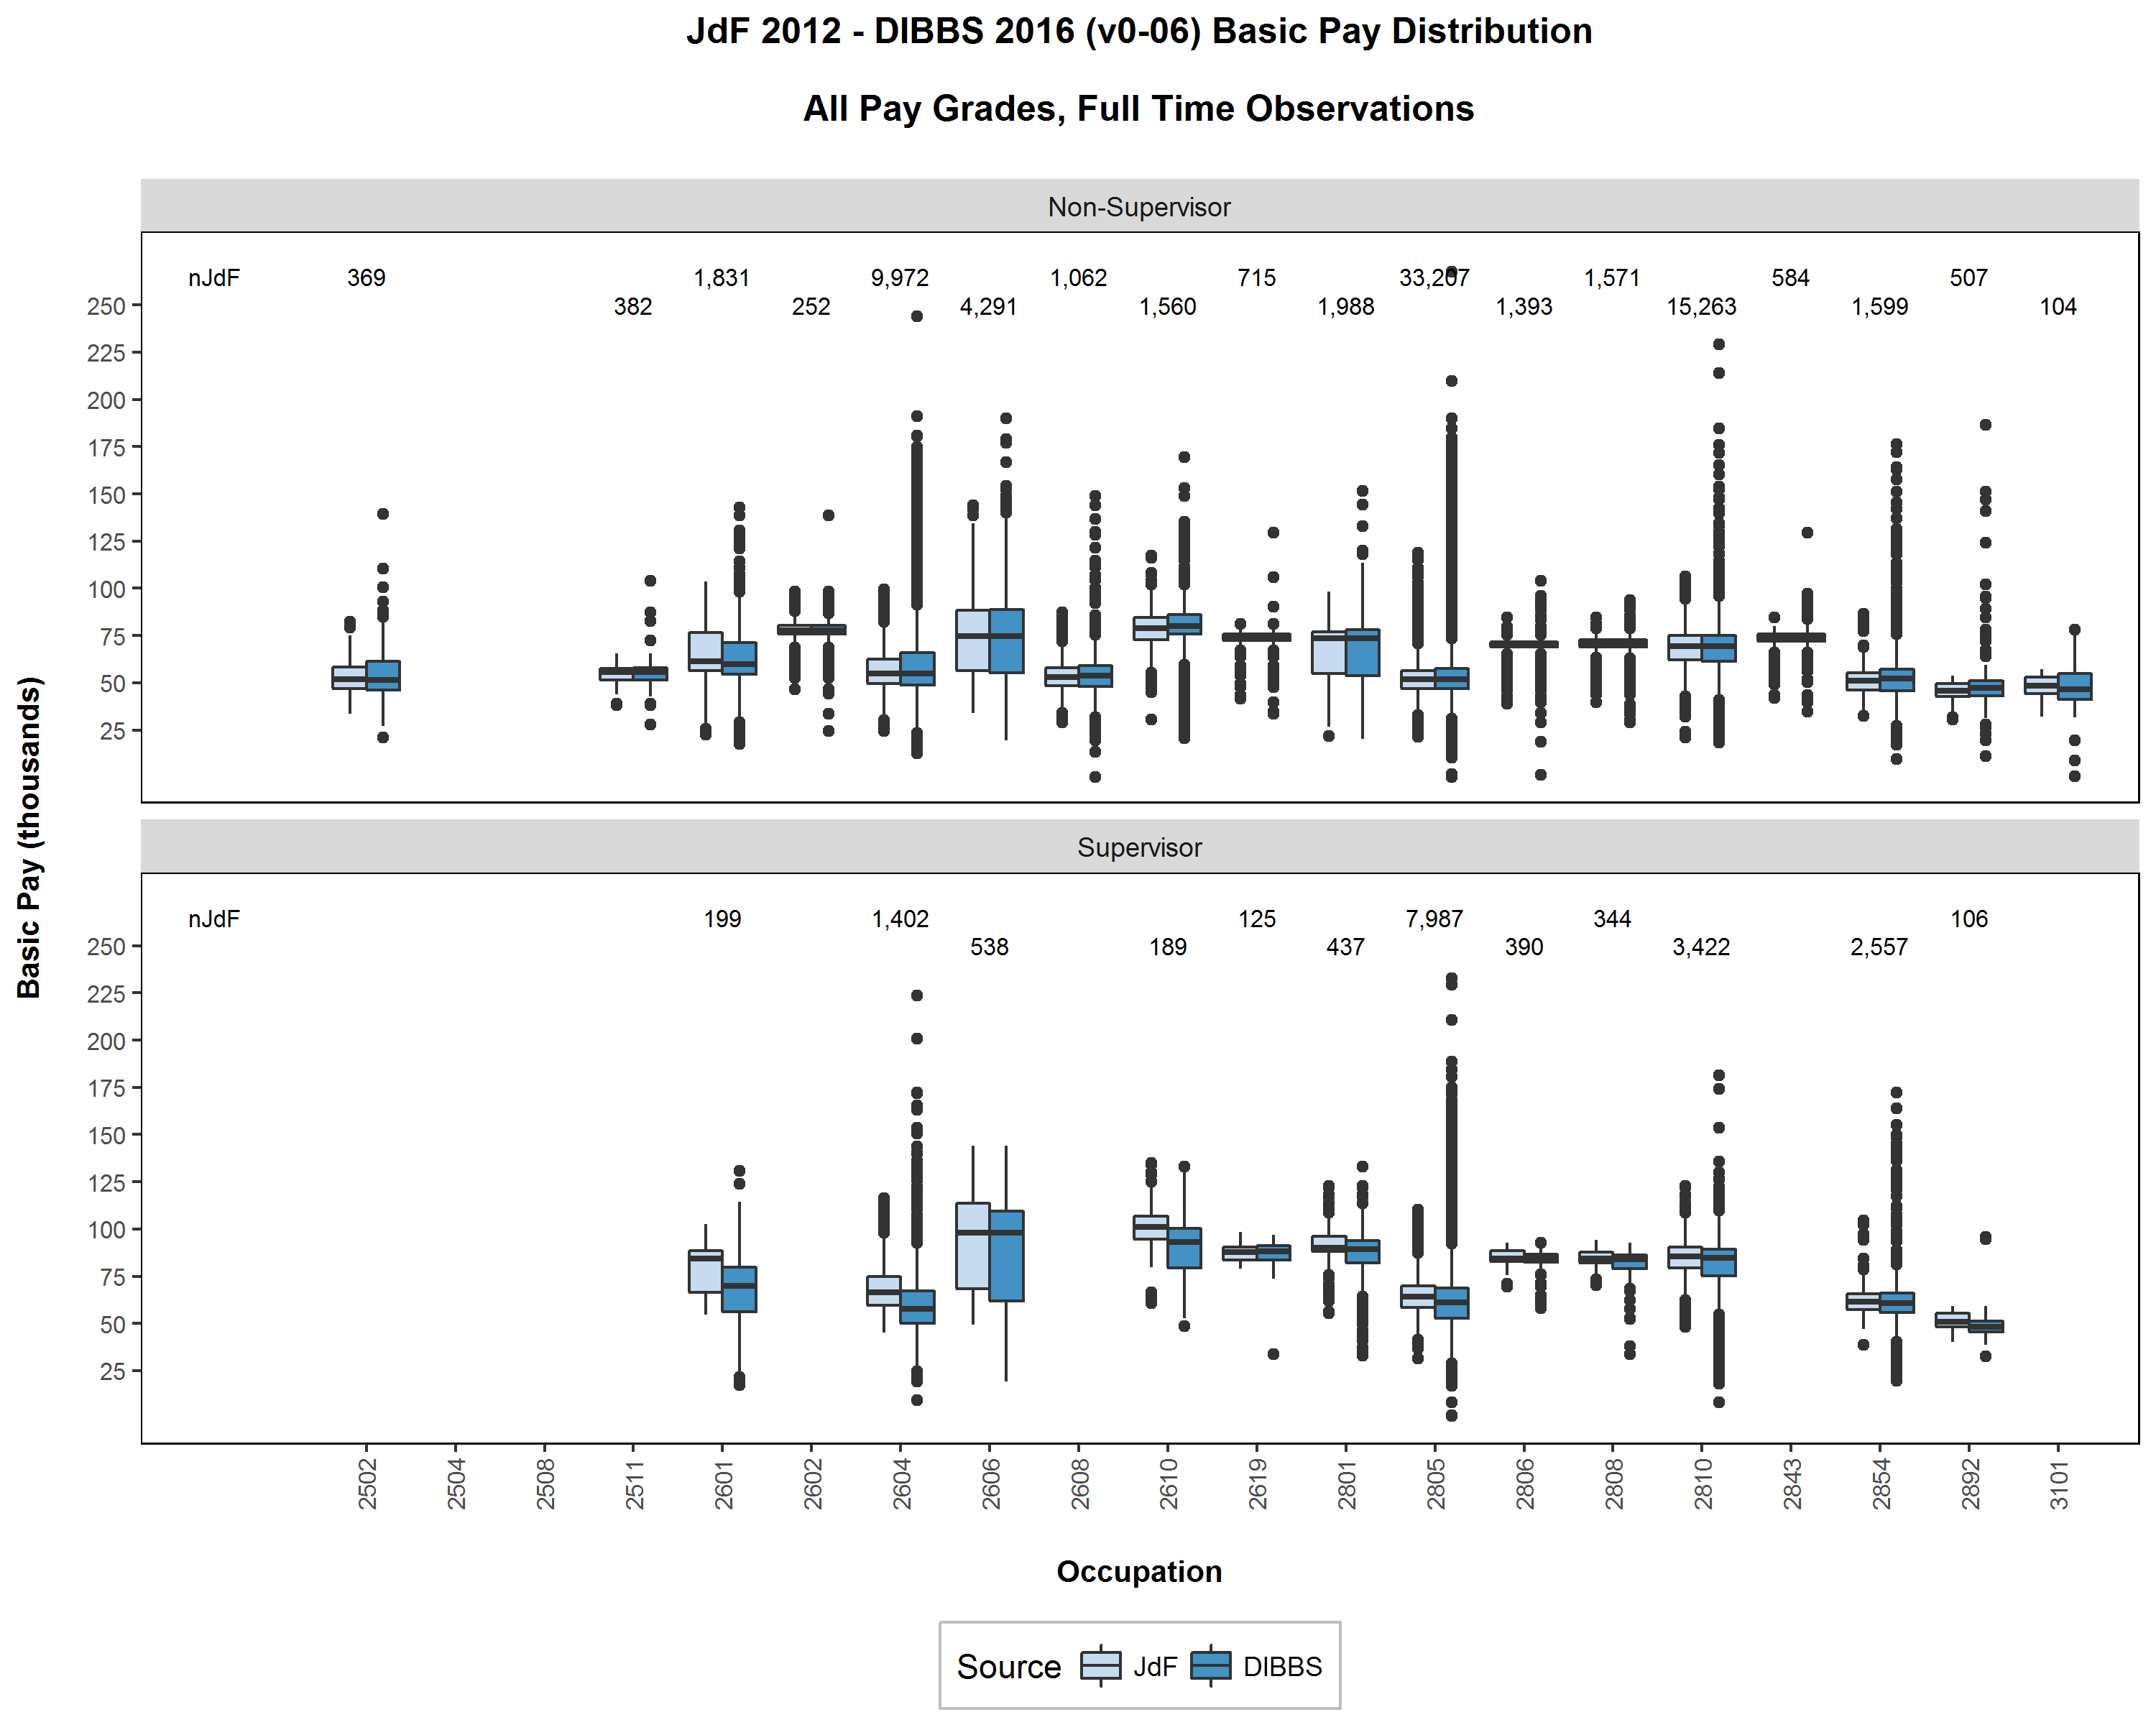
\includegraphics[width=6in, trim={0 1in 0 0.75in}, clip]{JdFDIBBSBasicPaySupervisoryStatusOccupation481.png}
        \caption{Occupations 2502 through 3101 (trades)}
        \vspace{10pt}
    \end{subfigure}
    \begin{subfigure}{1\textwidth}
        \centering
        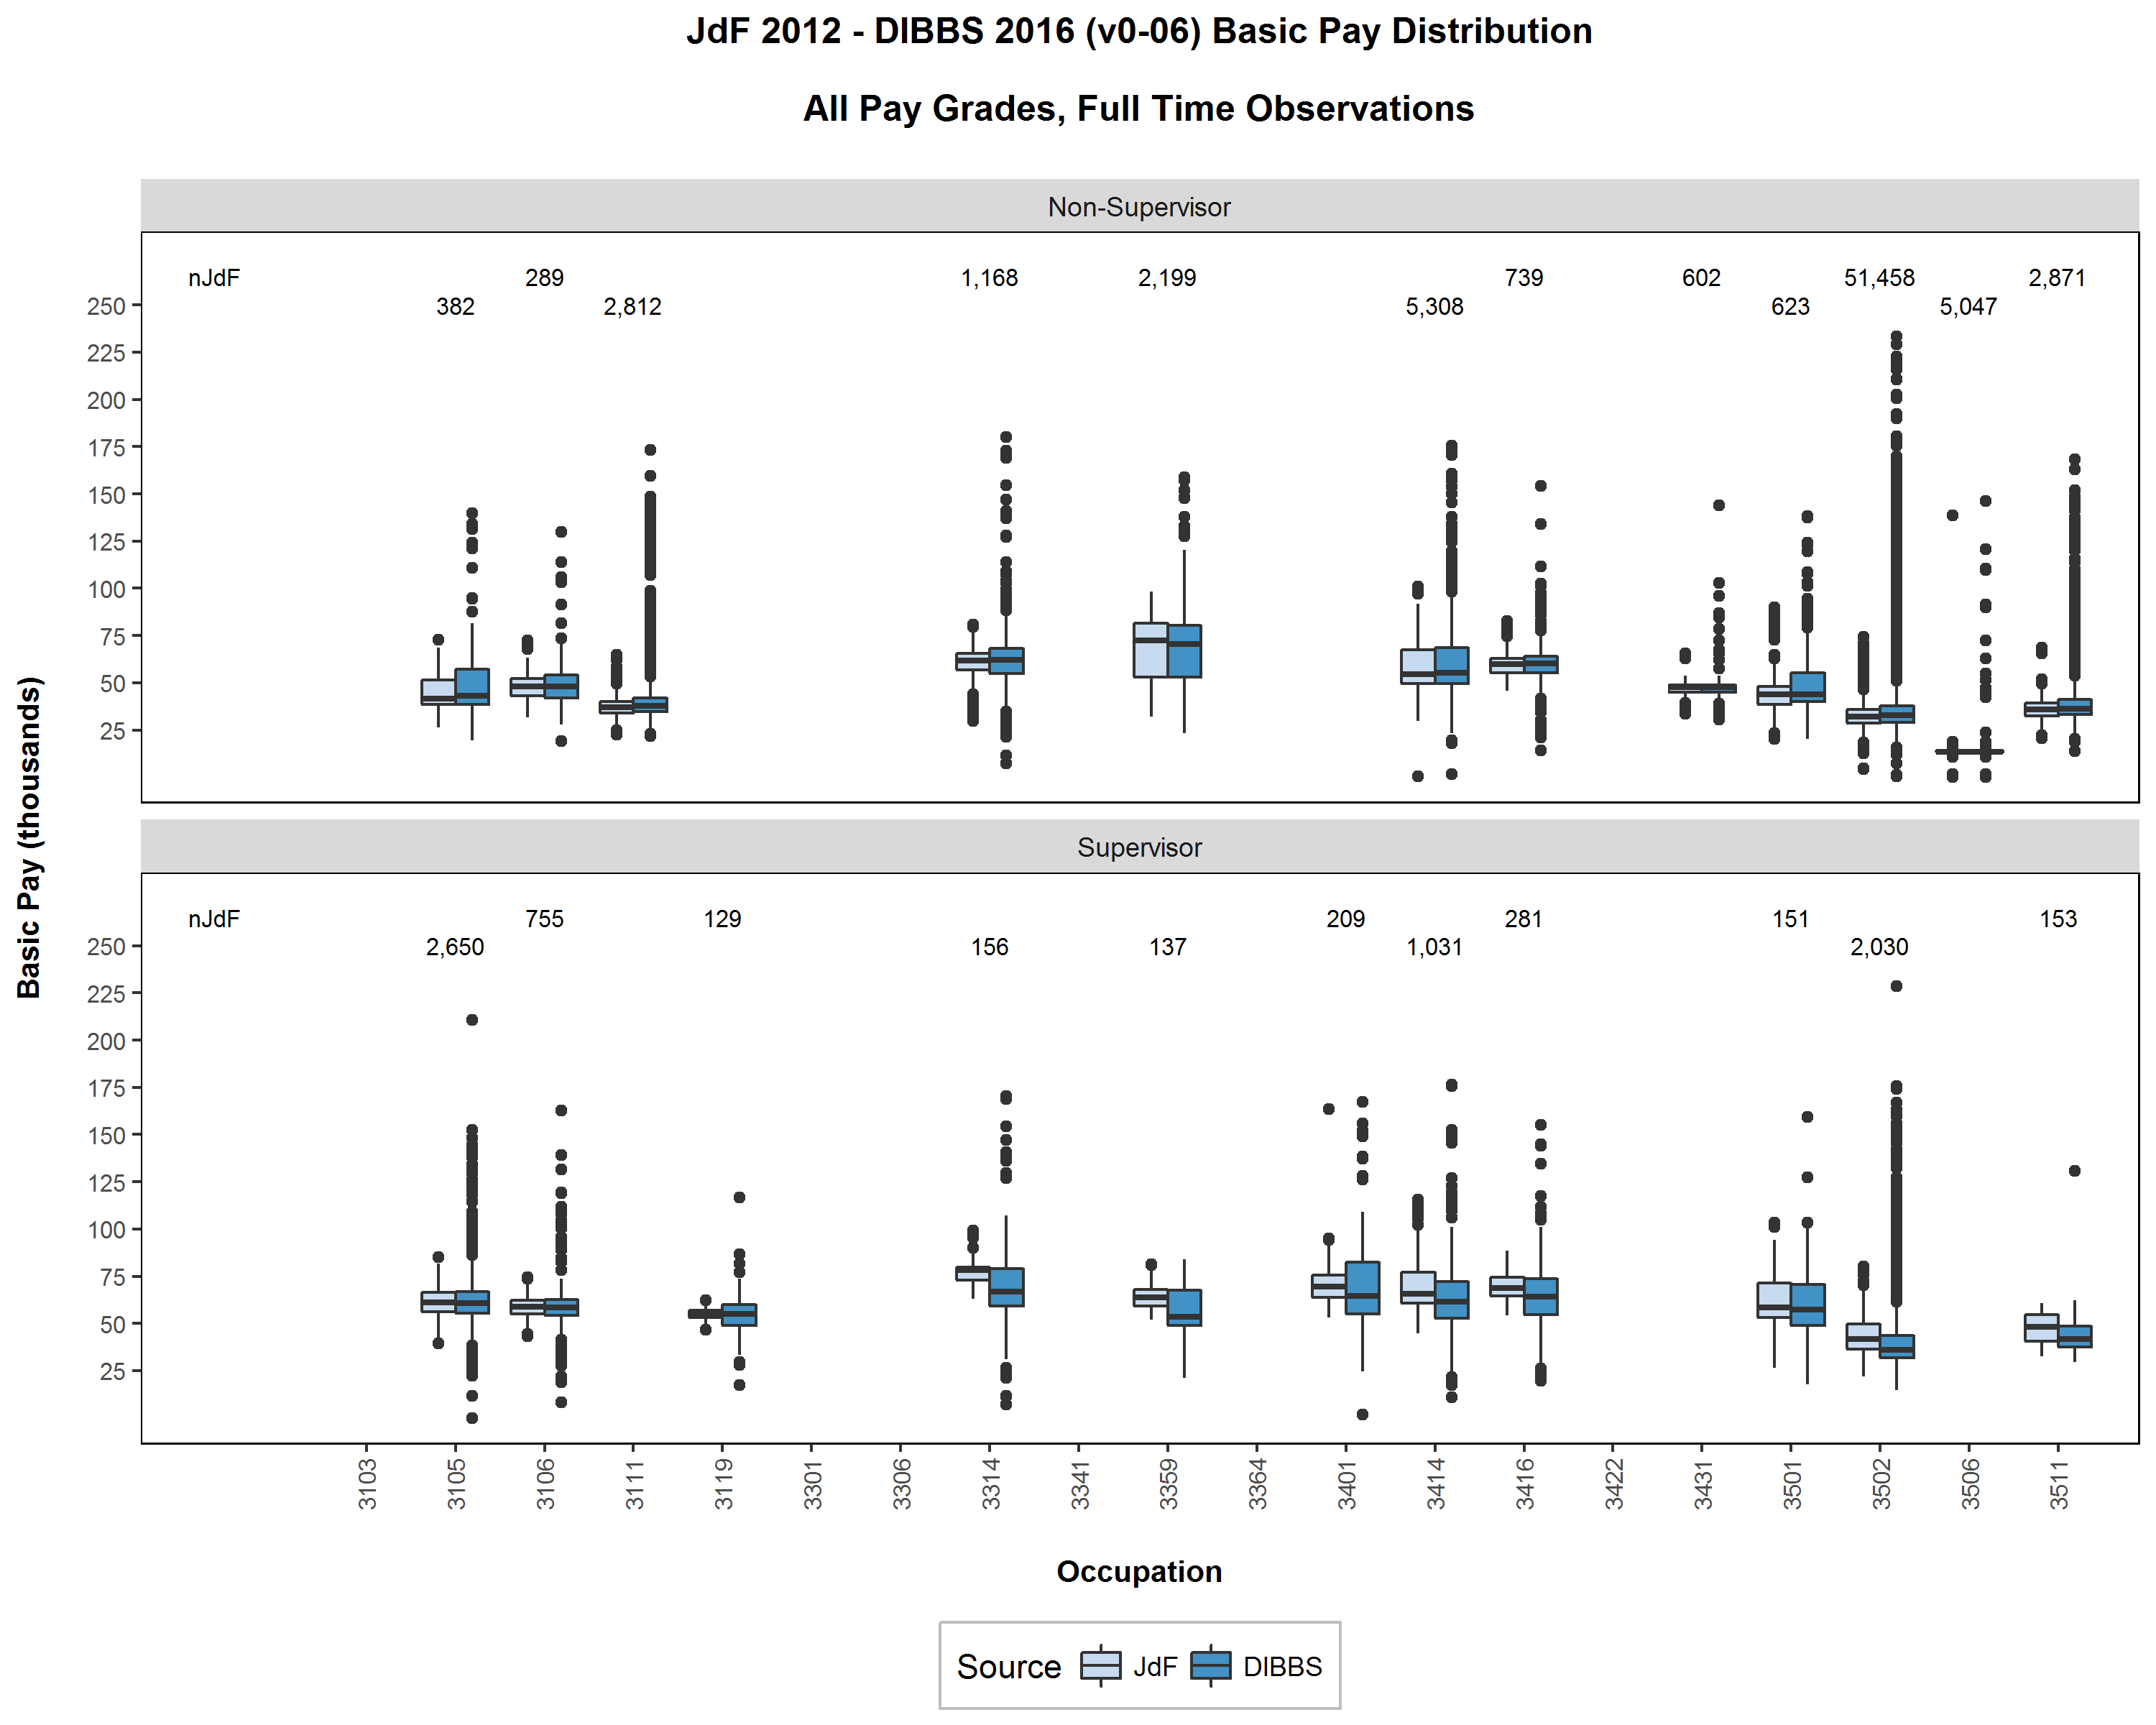
\includegraphics[width=6in, trim={0 1in 0 0.75in}, clip]{JdFDIBBSBasicPaySupervisoryStatusOccupation501.png}
        \caption{Occupations 3103 through 3511 (trades)}
        \vspace{10pt}
    \end{subfigure}
    \caption{Basic pay distribution by occupation and supervisor status.  All agencies combined.  Authentic boxes on left, synthetic on right.}
    \label{figure:JdFDIBBSBasicPaySupervisoryStatusOccupation4}
\end{figure}

\clearpage

\begin{figure}[h]
    \centering
    \begin{subfigure}{1\textwidth}
        \centering
        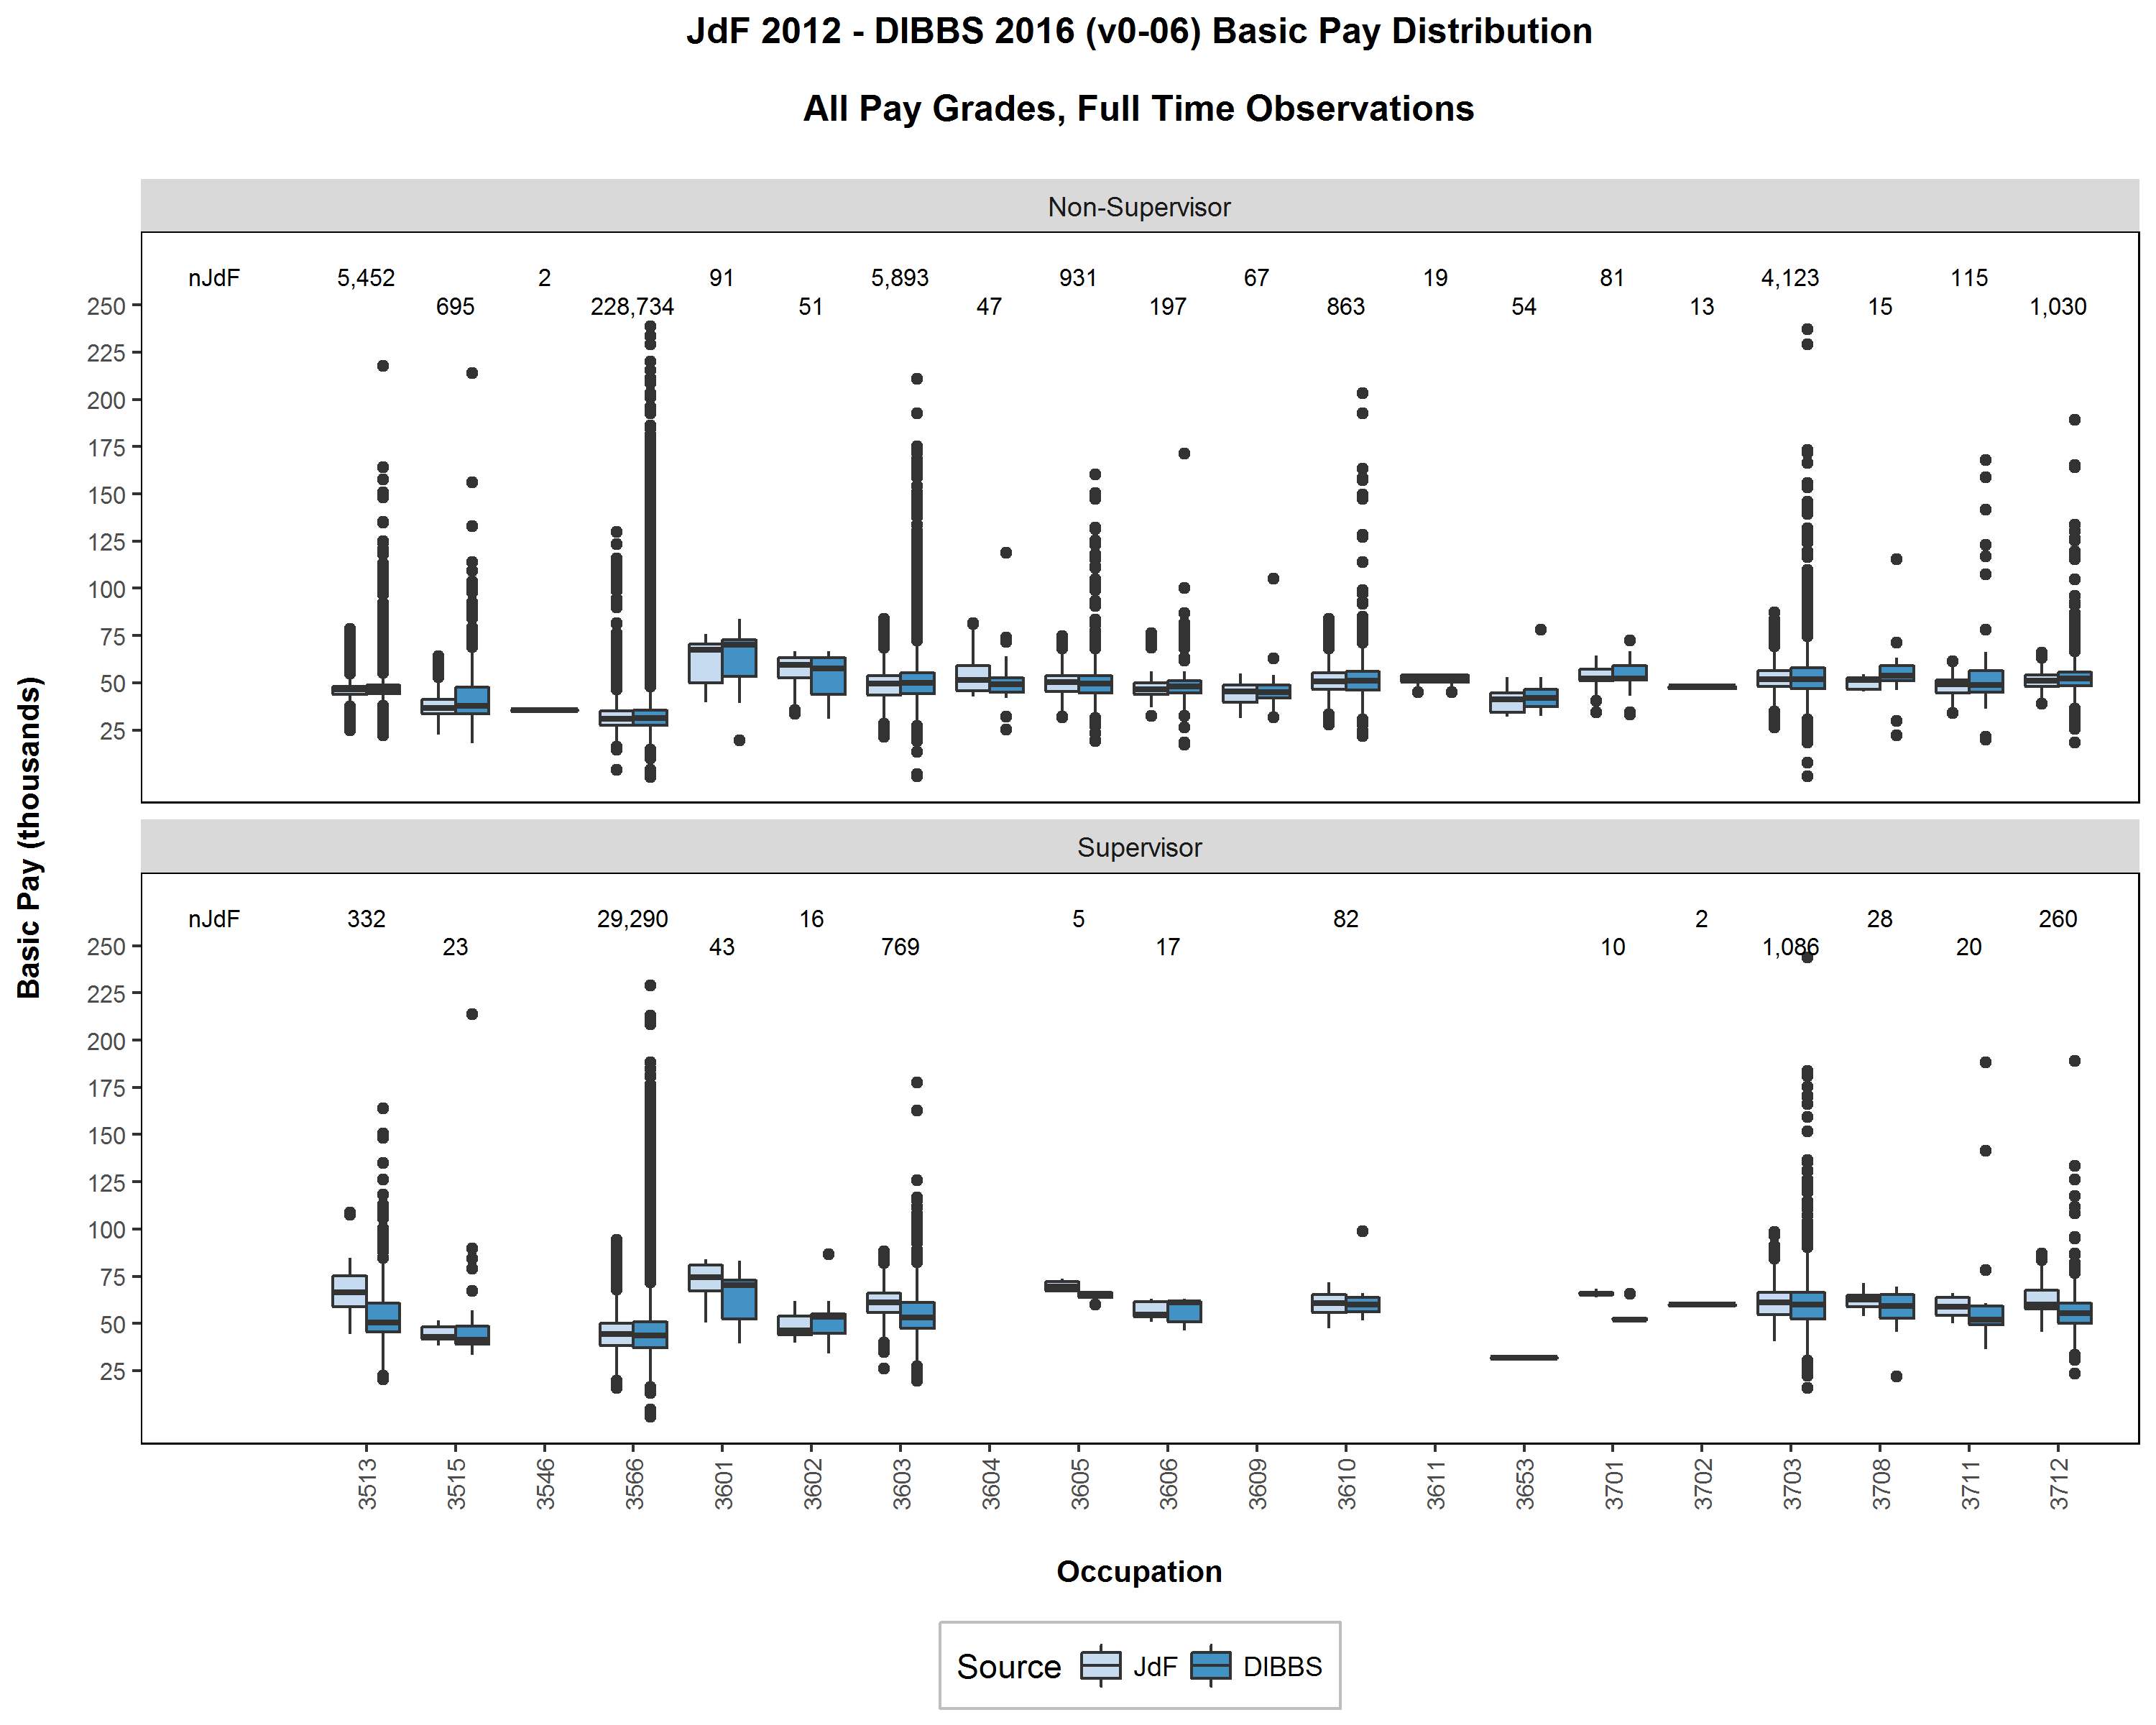
\includegraphics[width=6in, trim={0 1in 0 0.75in}, clip]{JdFDIBBSBasicPaySupervisoryStatusOccupation521.png}
        \caption{Occupations 3513 through 3712 (trades)}
        \vspace{10pt}
    \end{subfigure}
    \begin{subfigure}{1\textwidth}
        \centering
        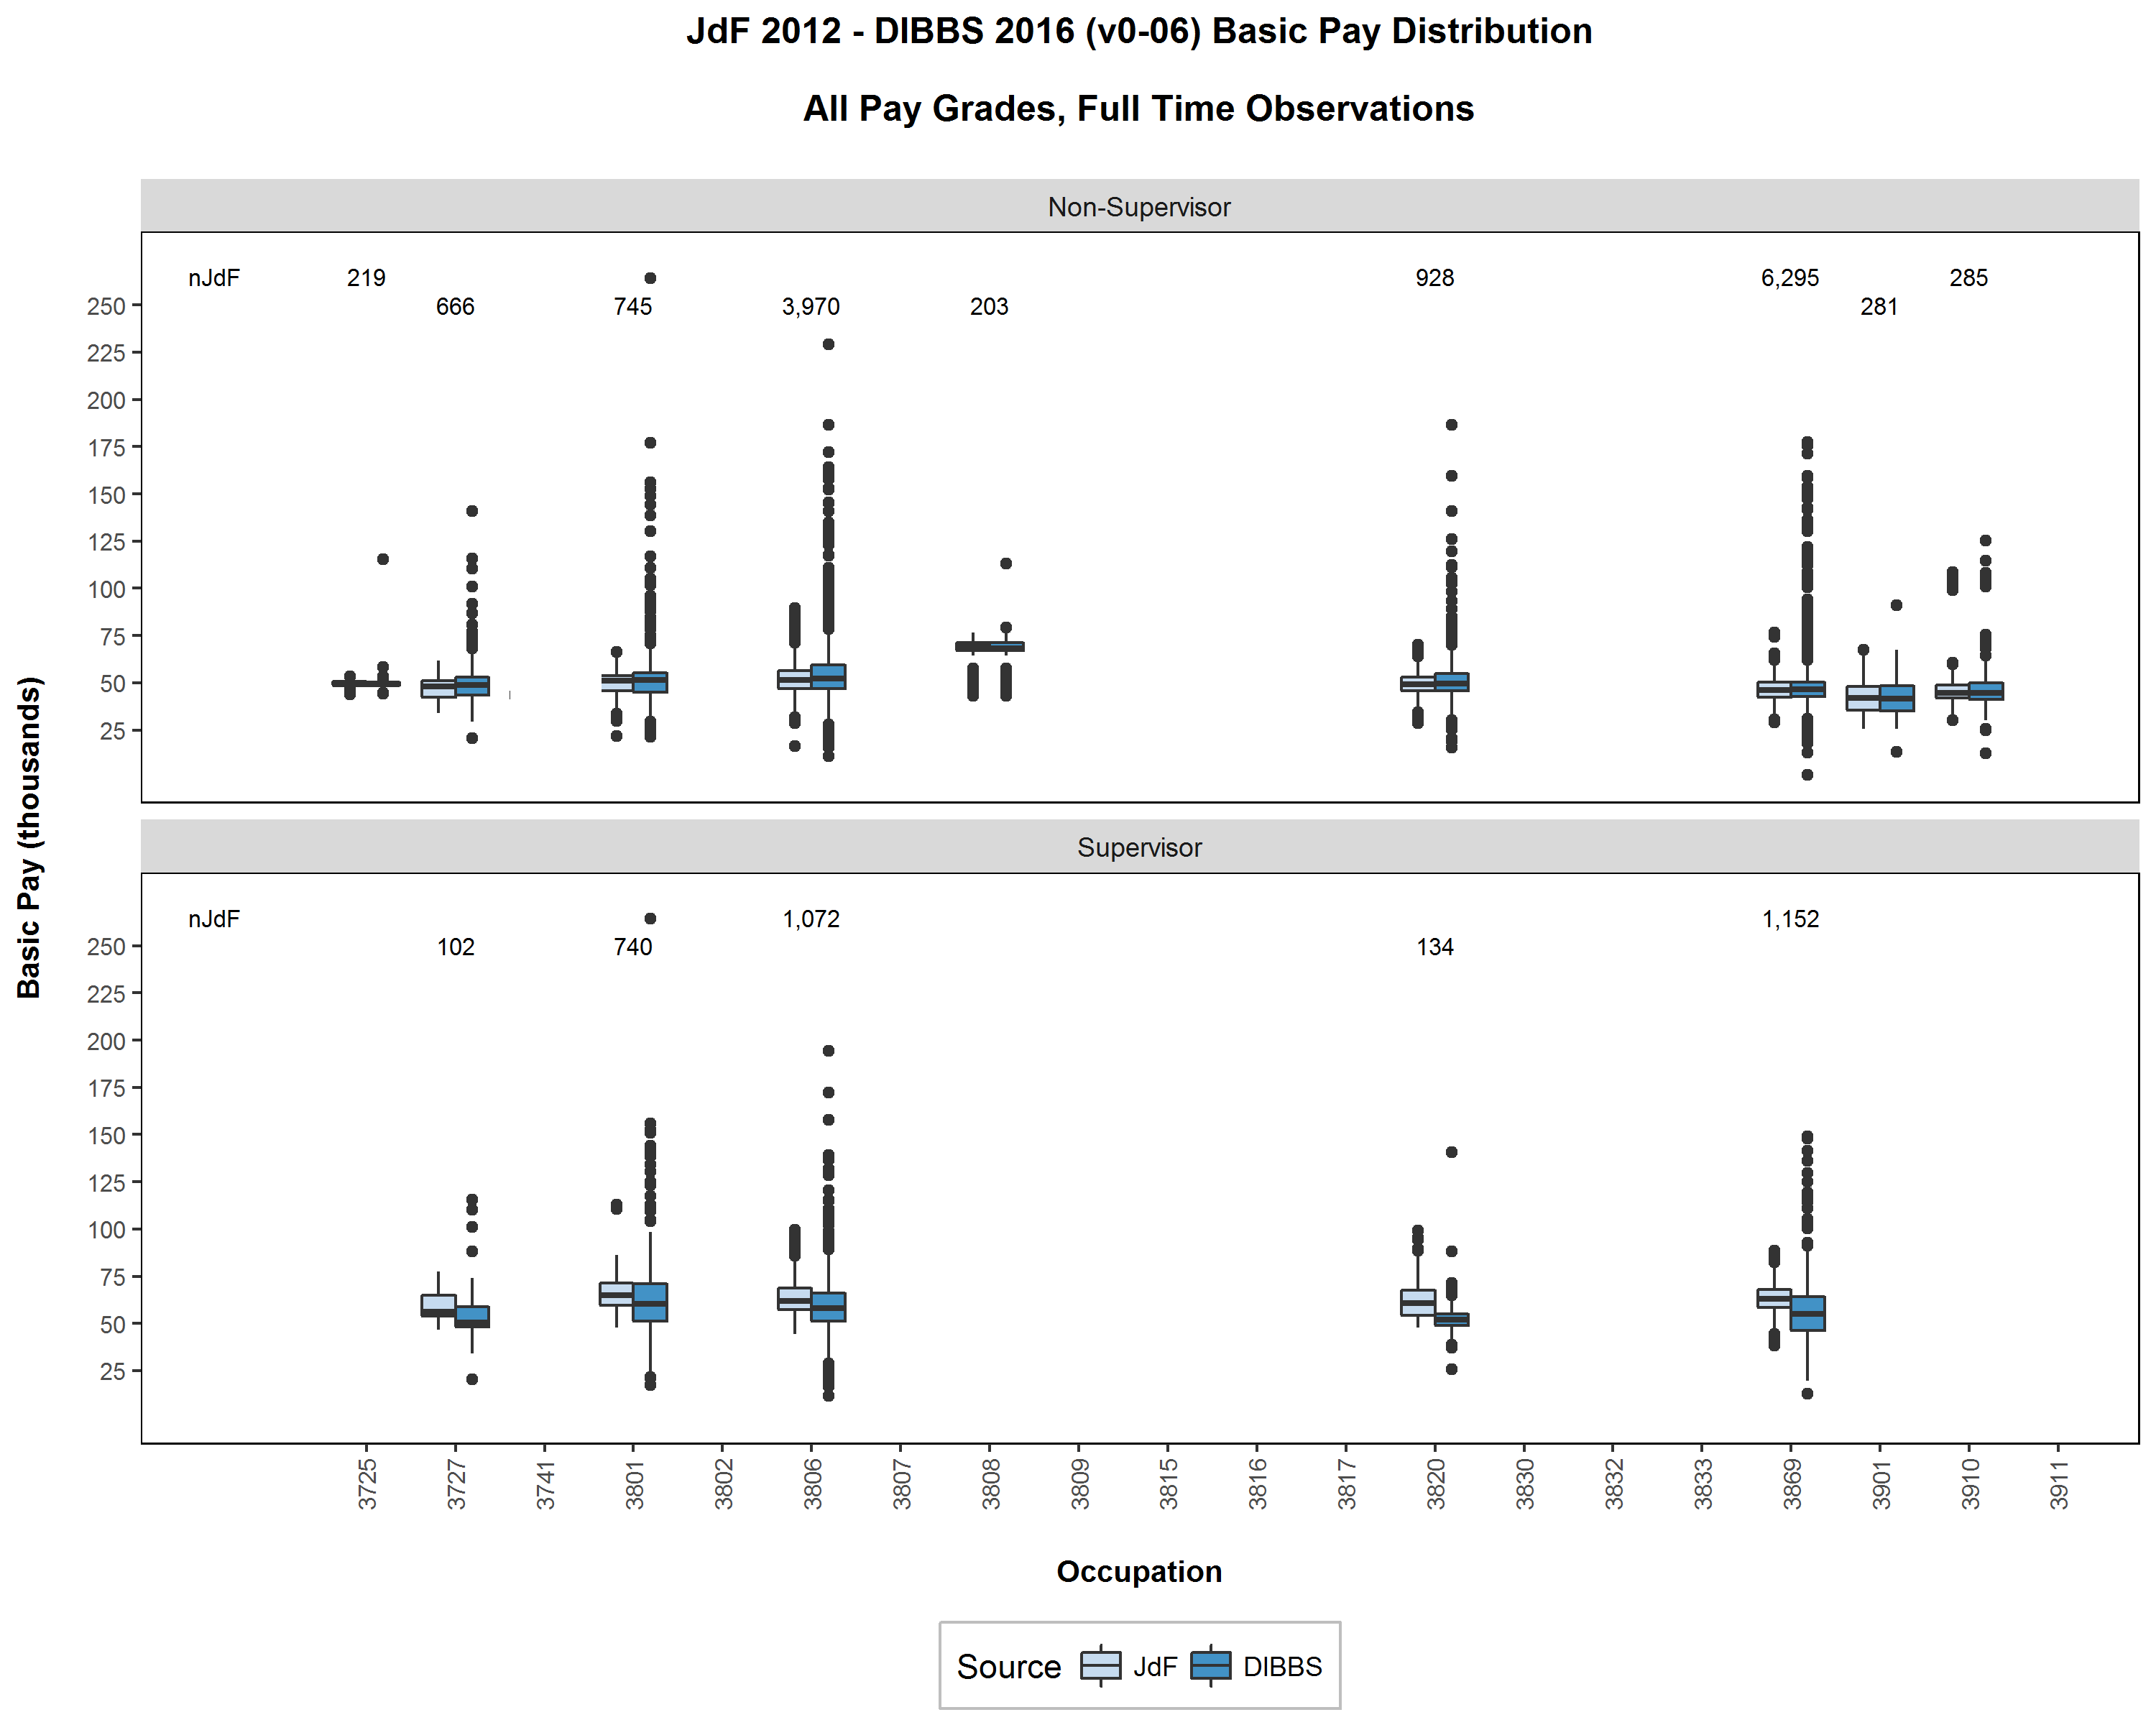
\includegraphics[width=6in, trim={0 1in 0 0.75in}, clip]{JdFDIBBSBasicPaySupervisoryStatusOccupation541.png}
        \caption{Occupations 3725 through 3911 (trades}
        \vspace{10pt}
    \end{subfigure}
    \caption{Basic pay distribution by occupation and supervisor status.  All agencies combined.  Authentic boxes on left, synthetic on right.}
    \label{figure:JdFDIBBSBasicPaySupervisoryStatusOccupation5}
\end{figure}

\clearpage

MEAN LOG(BASIC PAY) BY GENDER, RACE, AND YEAR\\

The relationship of mean basic basic pay to joint combinations of sex, race, and year is important in human capital research and must be maintained in the synthetic data.  Figure \ref{figure:RaceLogPayBySex-FY} plots mean log(pay) by year for females (on left) and males (on right) for races Native American (A), Asian (B), black (C), Hispanic (D), and white (E).  Dashed lines for synthetic data, solid lines for authentic.\\

Observation:  Differentiating colors may not be visible, but apparent pairings of lines (dashed near solid following similar trends) form race pairs.  Although some systematic difference appears between data sets, inter-year and overall trends are very similar.

\vspace{12pt}

\begin{figure}[h!]
    \centering
    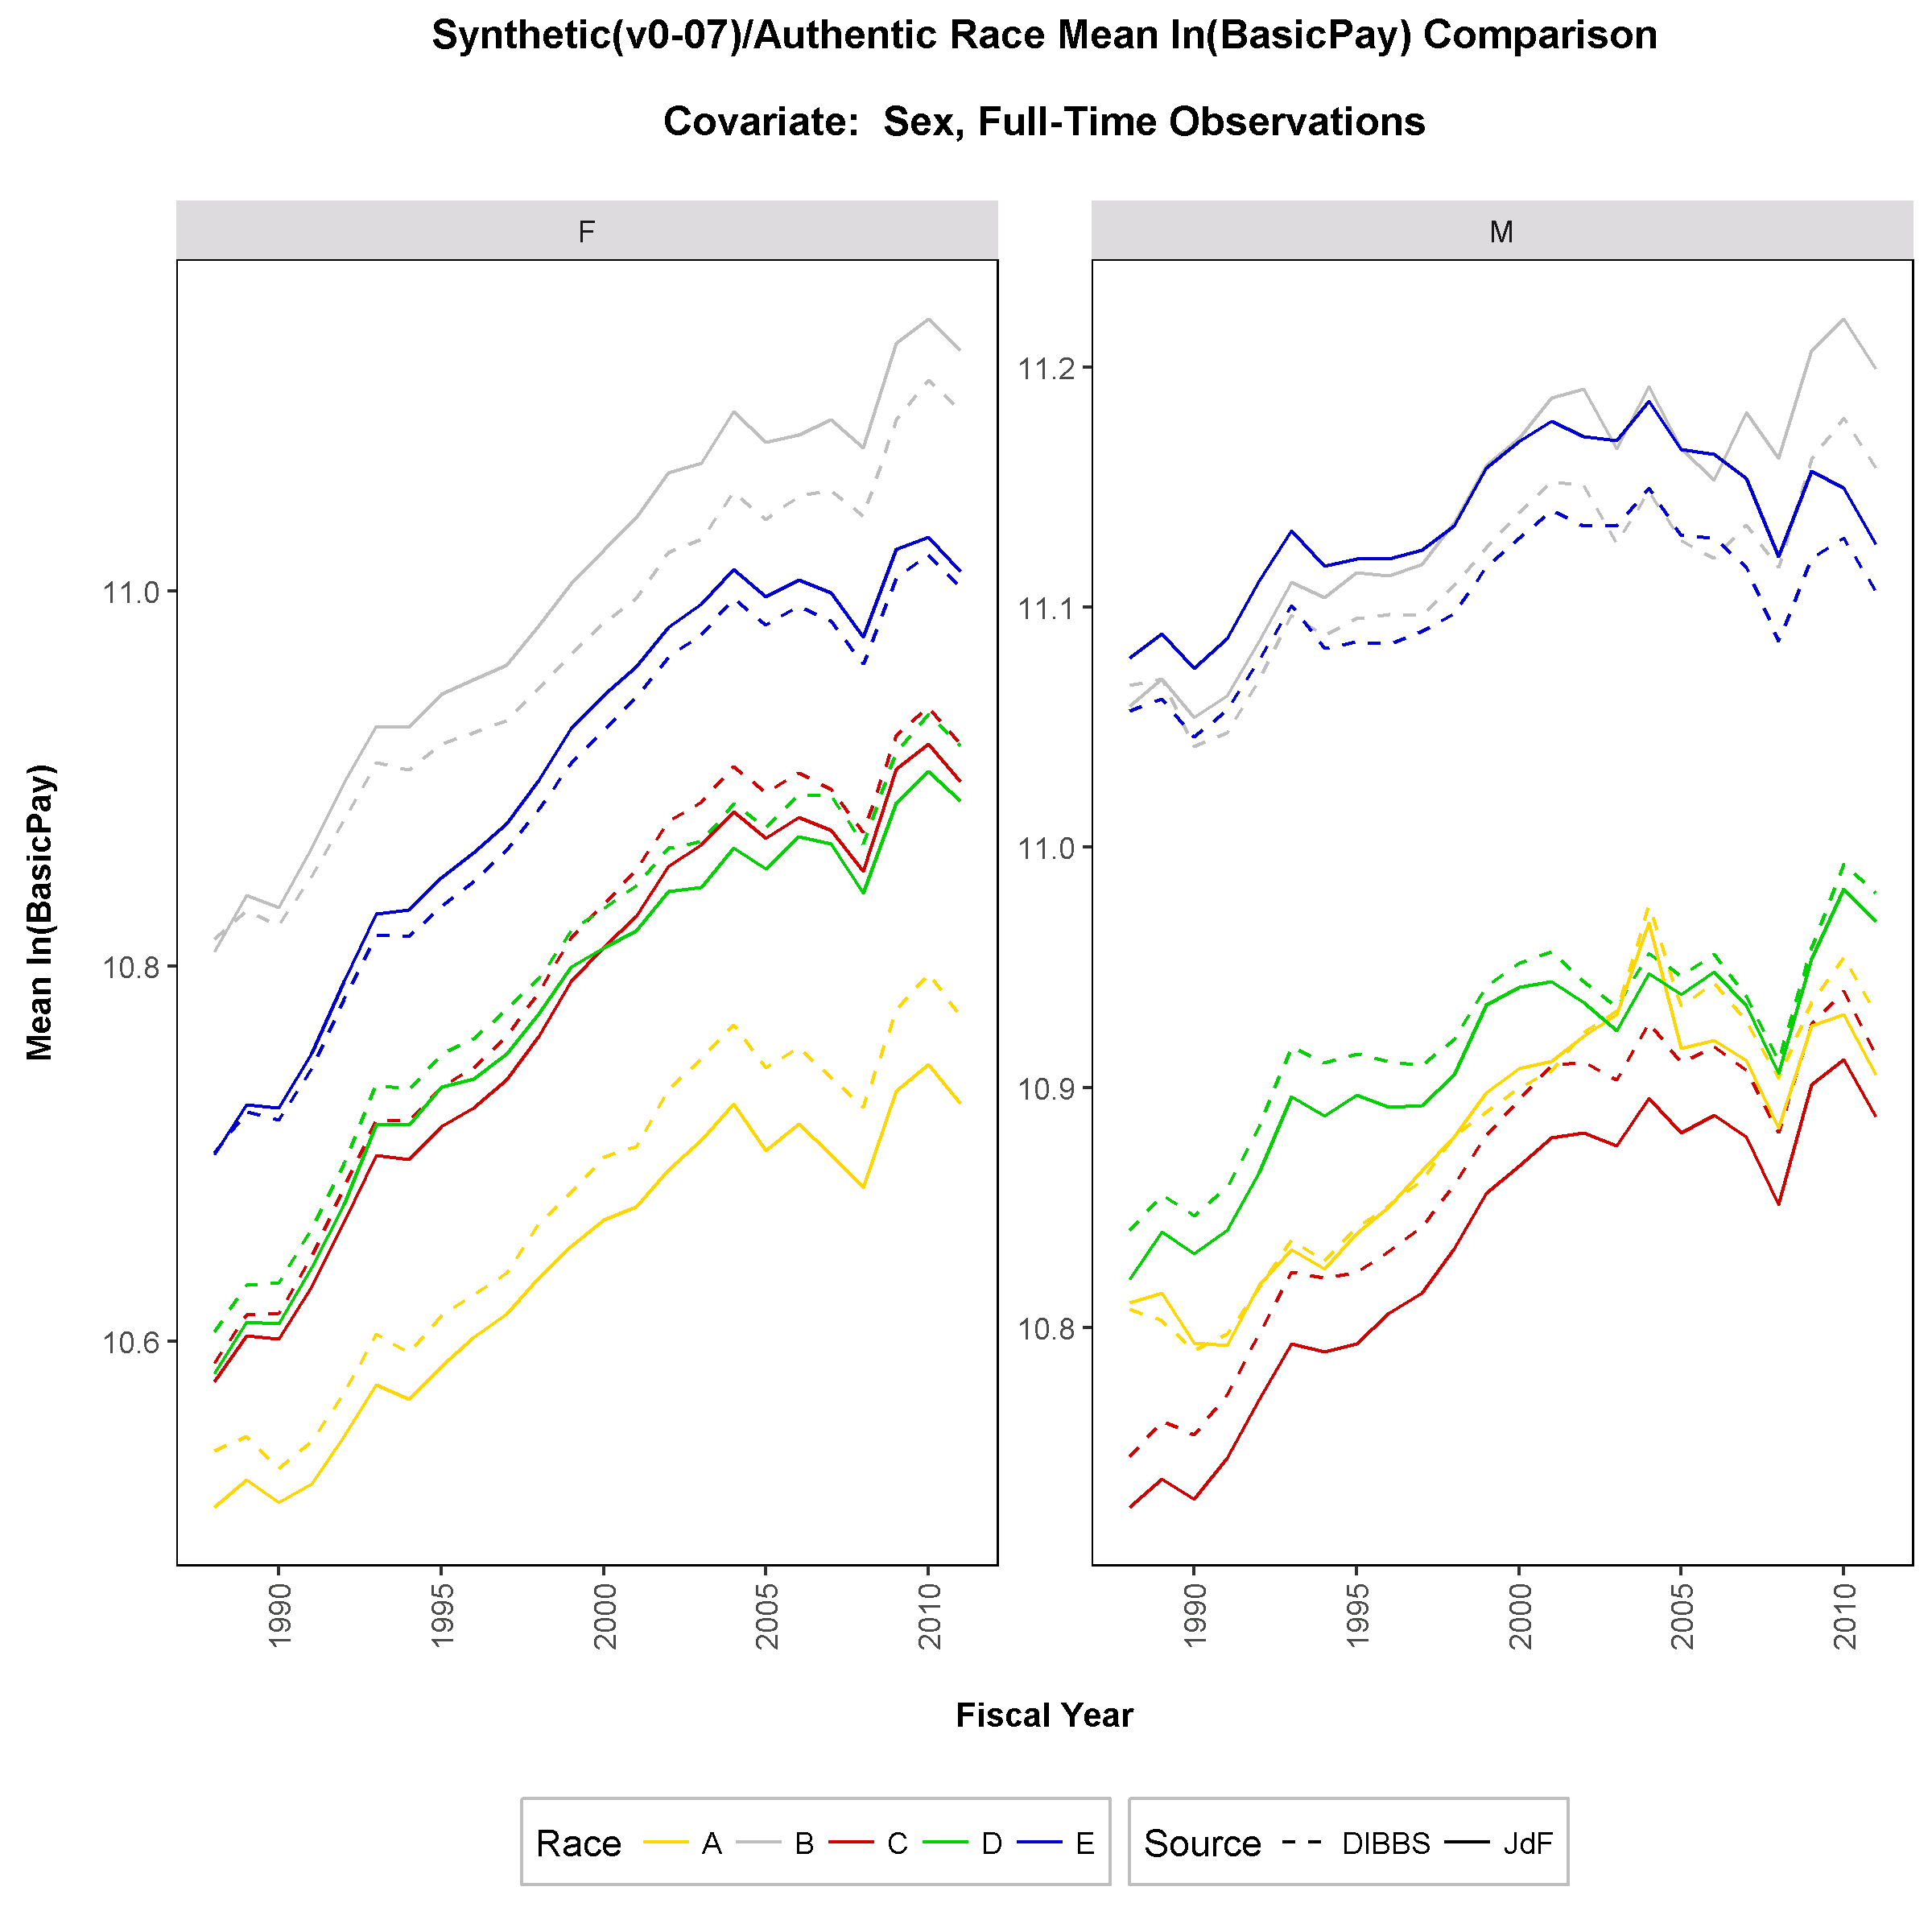
\includegraphics[width=6.5in, trim={0 0 0 0.75in}, clip]{RaceLogPayBySex-FY.png}
    \caption{Mean basic pay by sex, race, and year.  Female on left, male on right.  Race codes:  A = Native American, B = Asian, C = black, D = Hispanic, E = white.  Dashed line for synthetic data, solid line for authentic.}
    \label{figure:RaceLogPayBySex-FY}
\end{figure}

\clearpage

GENDER PAY DIFFERENTIAL FIXED EFFECTS QUANTILE REGRESSION MODEL\\

Figure \ref{figure:GenderPayDifferentialQuantileRegressionAgeRaceEdPanelv0-06} plots the 0.1, 0.5, and 0.9 quantile estimates of difference in log(basic pay) between federal employee women and men by year, controlled for race, age, education, agency, and occupation.\\

Observation:  Although some systematic separation appears between data sets, trends indicate similar proportion change with respect to time.

\vspace{20pt}

\begin{figure}[h!]
    \centering
    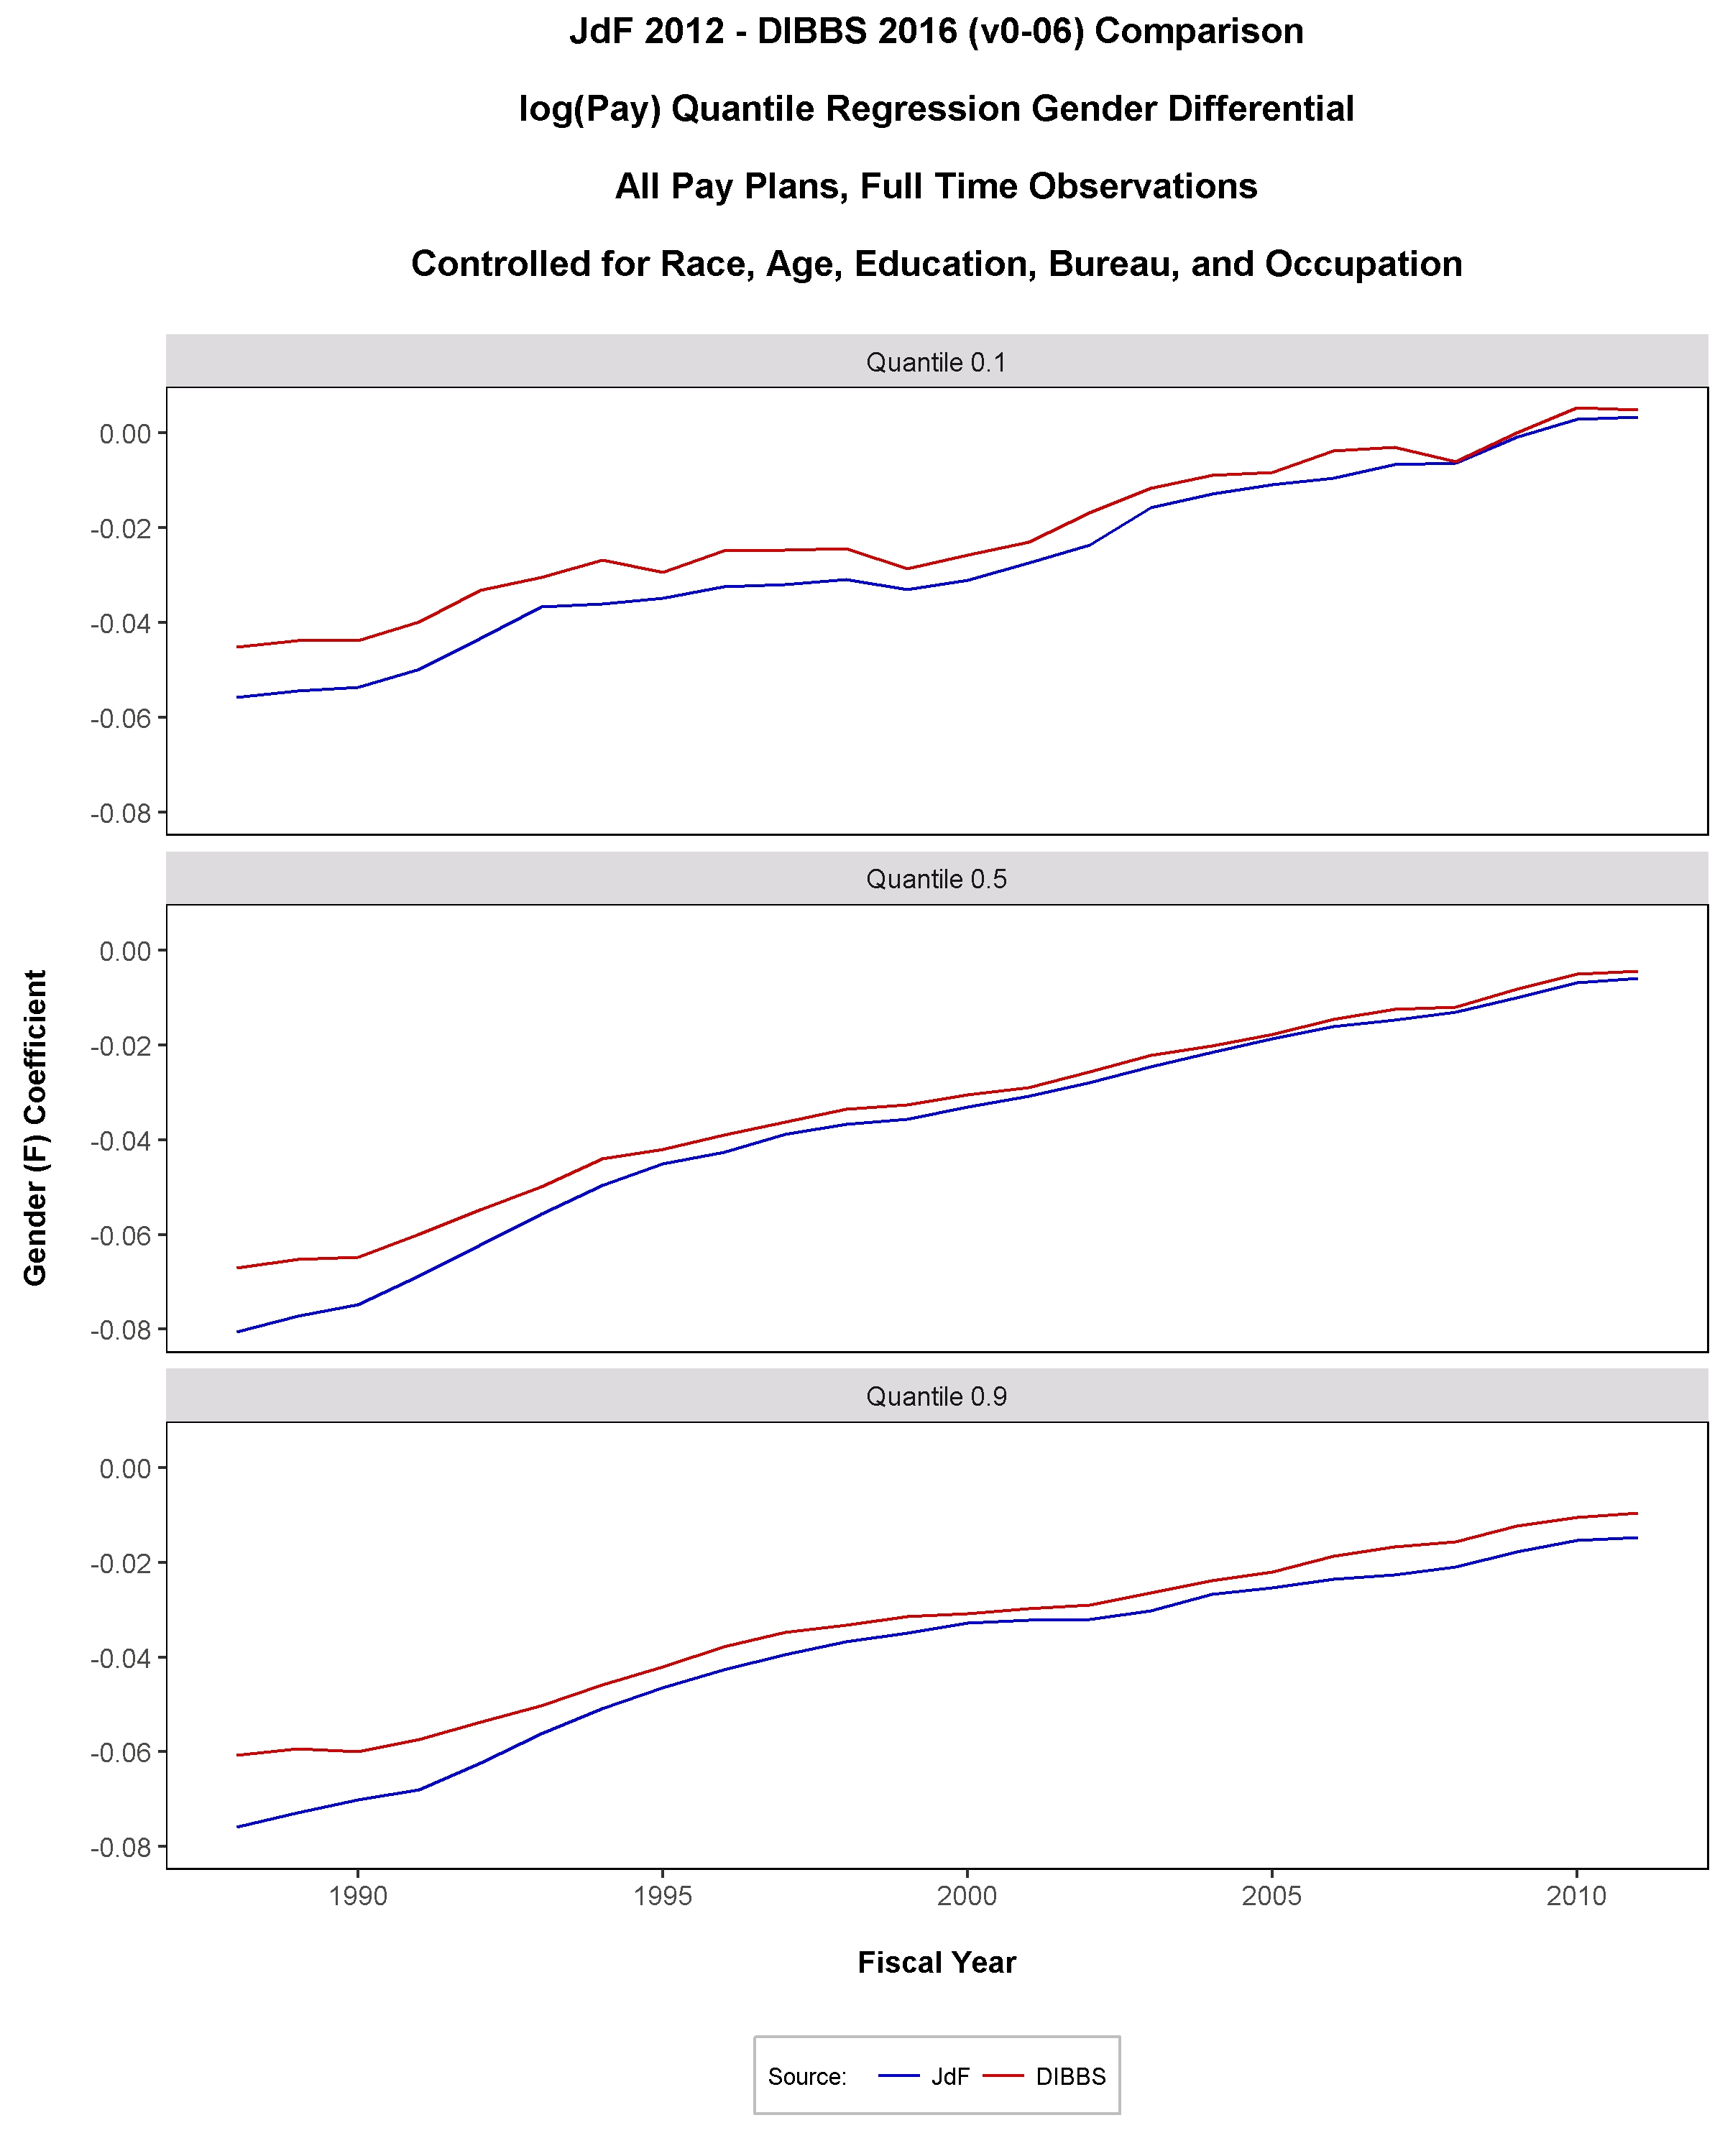
\includegraphics[width=6in, trim={0 0 0 1.5in}, clip]{GenderPayDifferentialQuantileRegressionAgeRaceEdPanelv0-06.png}
    \caption{Quantile estimates from gender pay disparity fixed effects model.  Upper line from synthetic data, lower line from authentic.}
    \label{figure:GenderPayDifferentialQuantileRegressionAgeRaceEdPanelv0-06}
\end{figure}

\clearpage

GENDER PROPORTION BY RACE, EDUCATION, AND YEAR\\

Proportion observations by gender is critical in models involving gender effects.  Figure \ref{figure:GenderProportionLogisticModelEducationRaceFYScaleFixedv0-06} plots proportion female employees by race, education, and year.  Fitted lines are logistic regression models.\\

Observation:  This four-way comparison (sex, race, education, and year) confirms good representation in synthetic data of gender proportion among important variable combinations in the authentic data.  Fitted logistic regression models have nearly identical trends through fiscal years.  Note the slight degradation in fit as observation count (n) decreases.\\

\vspace{20pt}

\begin{figure}[h!]
    \centering
    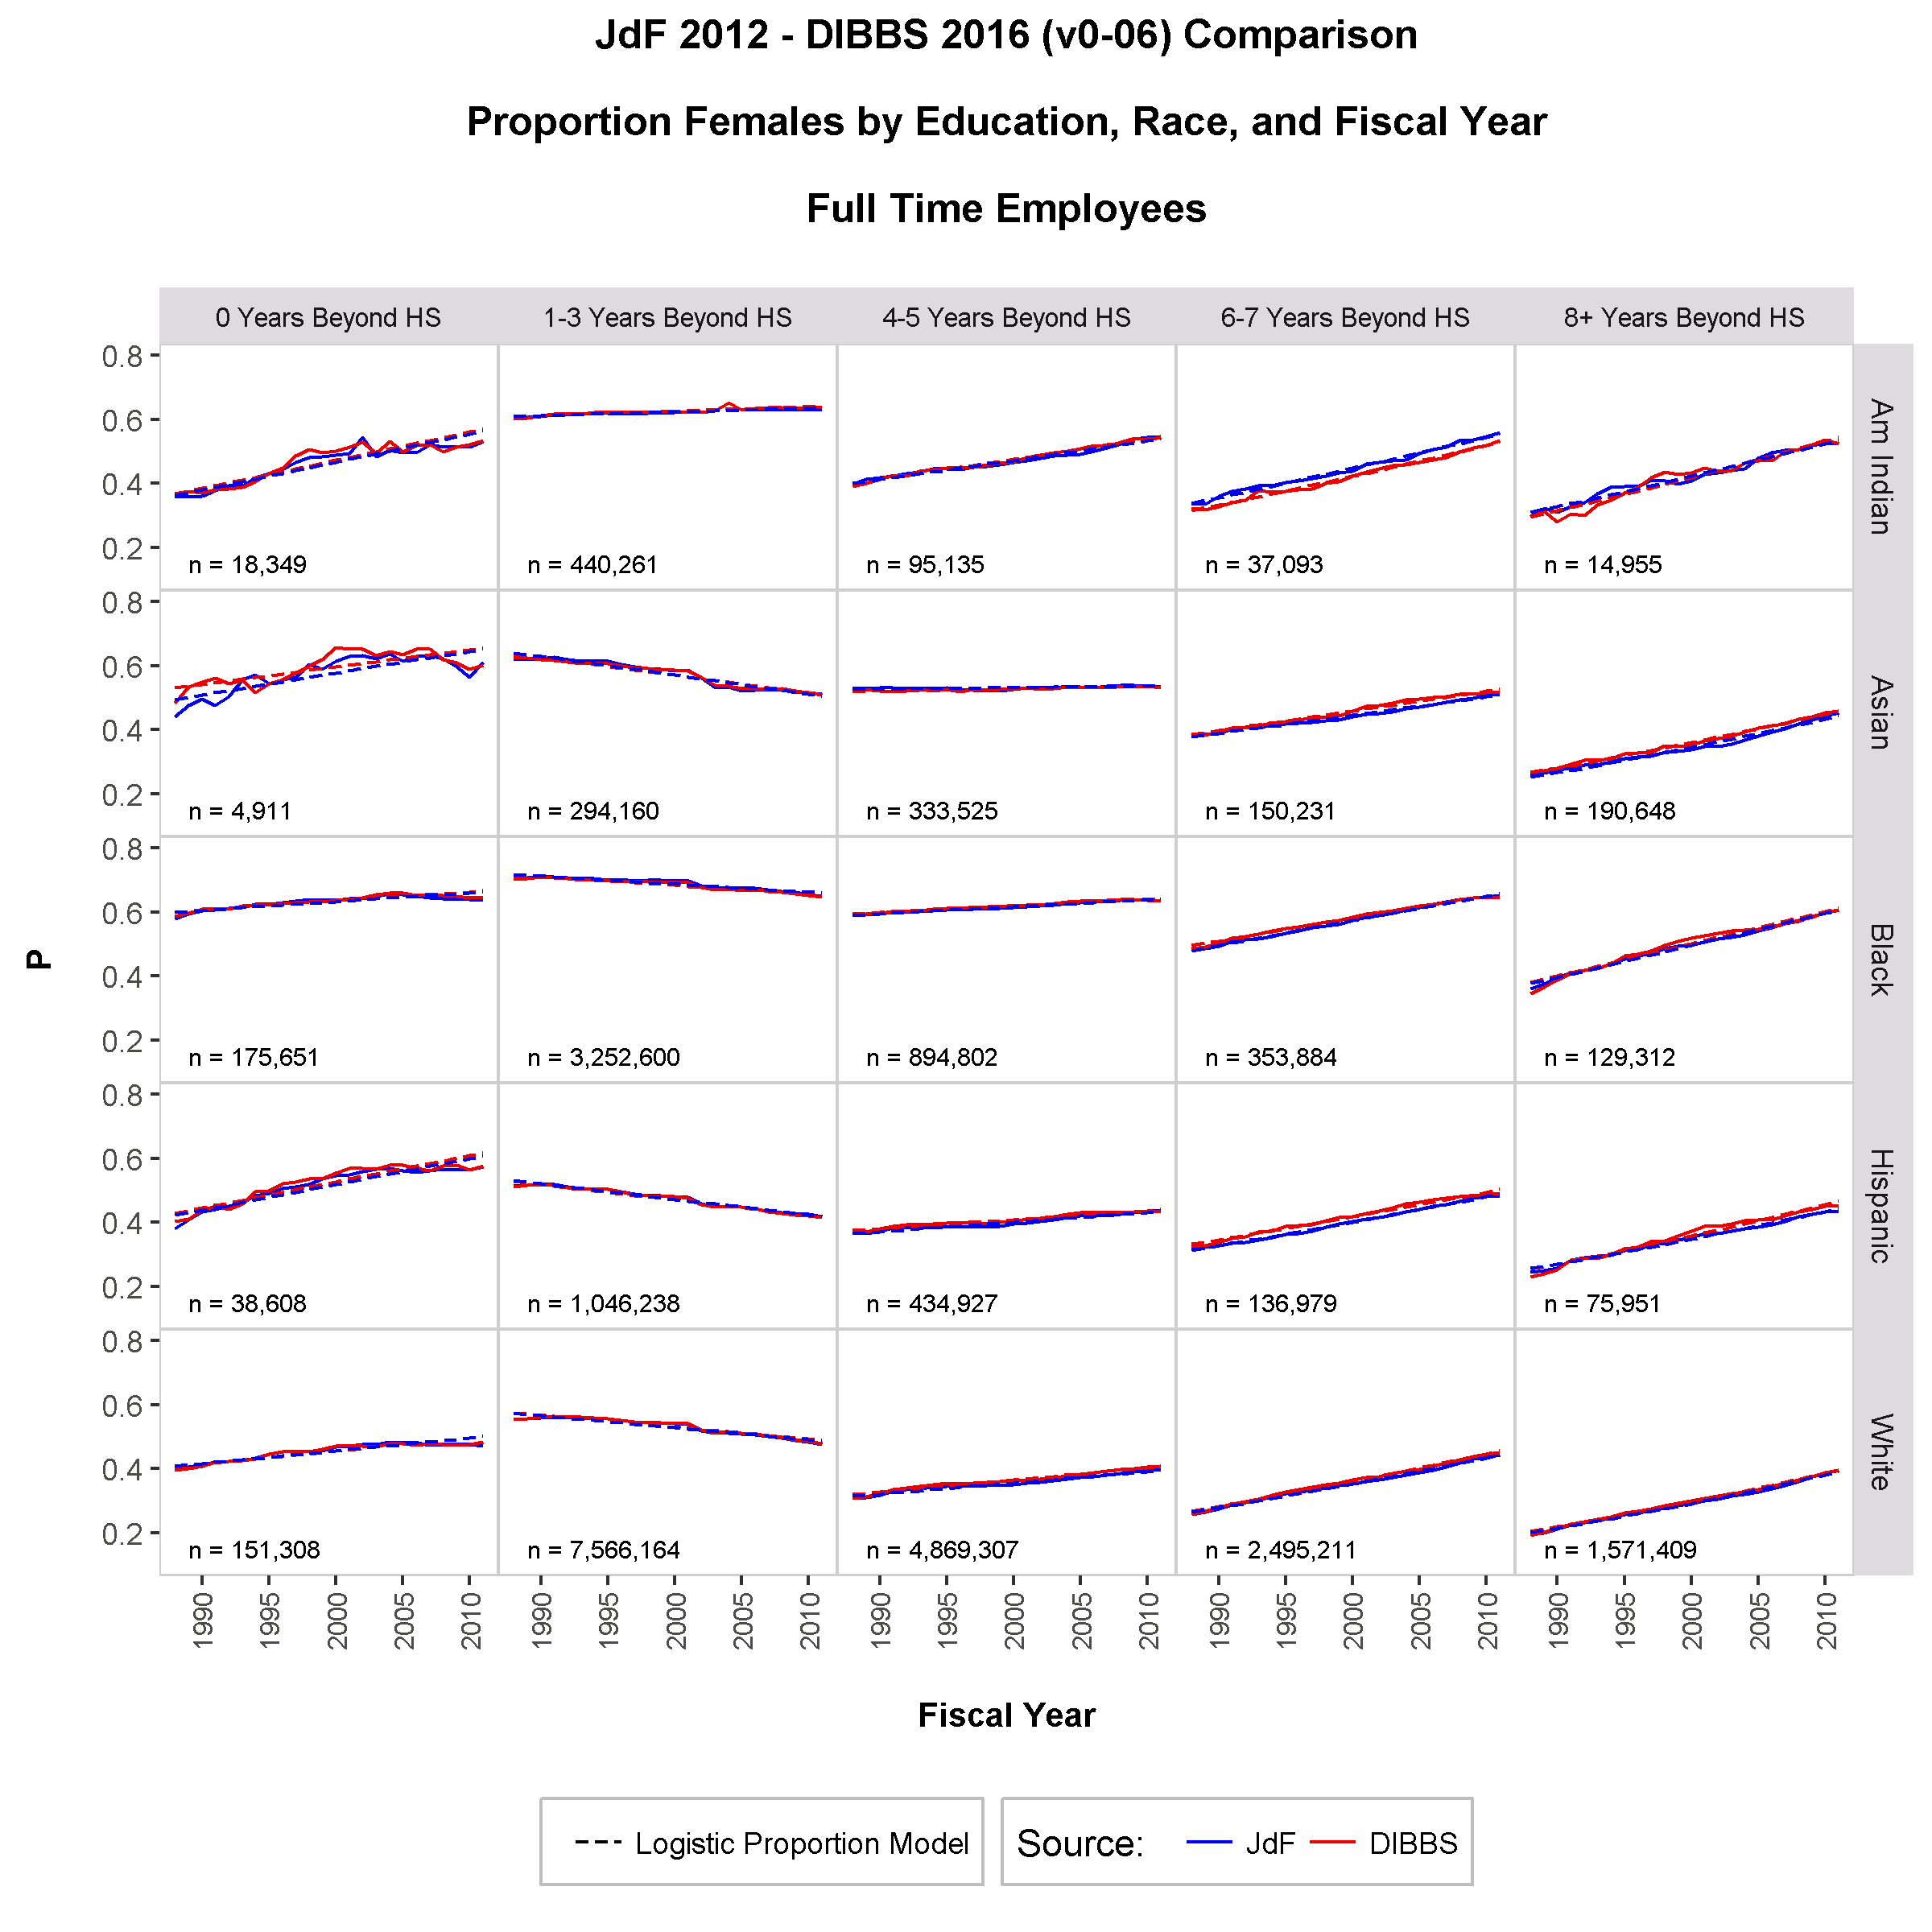
\includegraphics[width=6.5in, trim={0 0 0 1in}, clip]{GenderProportionLogisticModelEducationRaceFYScaleFixedv0-06.png}
    \caption{Proportion female observations by race, education, and year.  Fitted lines are logistic regression estimates.}
    \label{figure:GenderProportionLogisticModelEducationRaceFYScaleFixedv0-06}
\end{figure}

\clearpage

GENDER PROPORTION BY RACE, AGE, AND YEAR\\

Figures \ref{figure:GenderProportionLogisticModelFYRaceAgeA} through \ref{figure:GenderProportionLogisticModelFYRaceAgeE}, show for each race, proportion female employees by age and year.  Fitted lines are logistic regression models.\\

Observation:  These four-way comparisons (sex, race, age, and year) confirm good representation in synthetic data of gender proportion among important variable combinations in the authentic data.  Fitted logistic regression models have nearly identical trends through fiscal years.\\

Logistic models reveal agreement in trends between data sets.

\vspace{20pt}

\begin{figure}[h!]
    \centering
    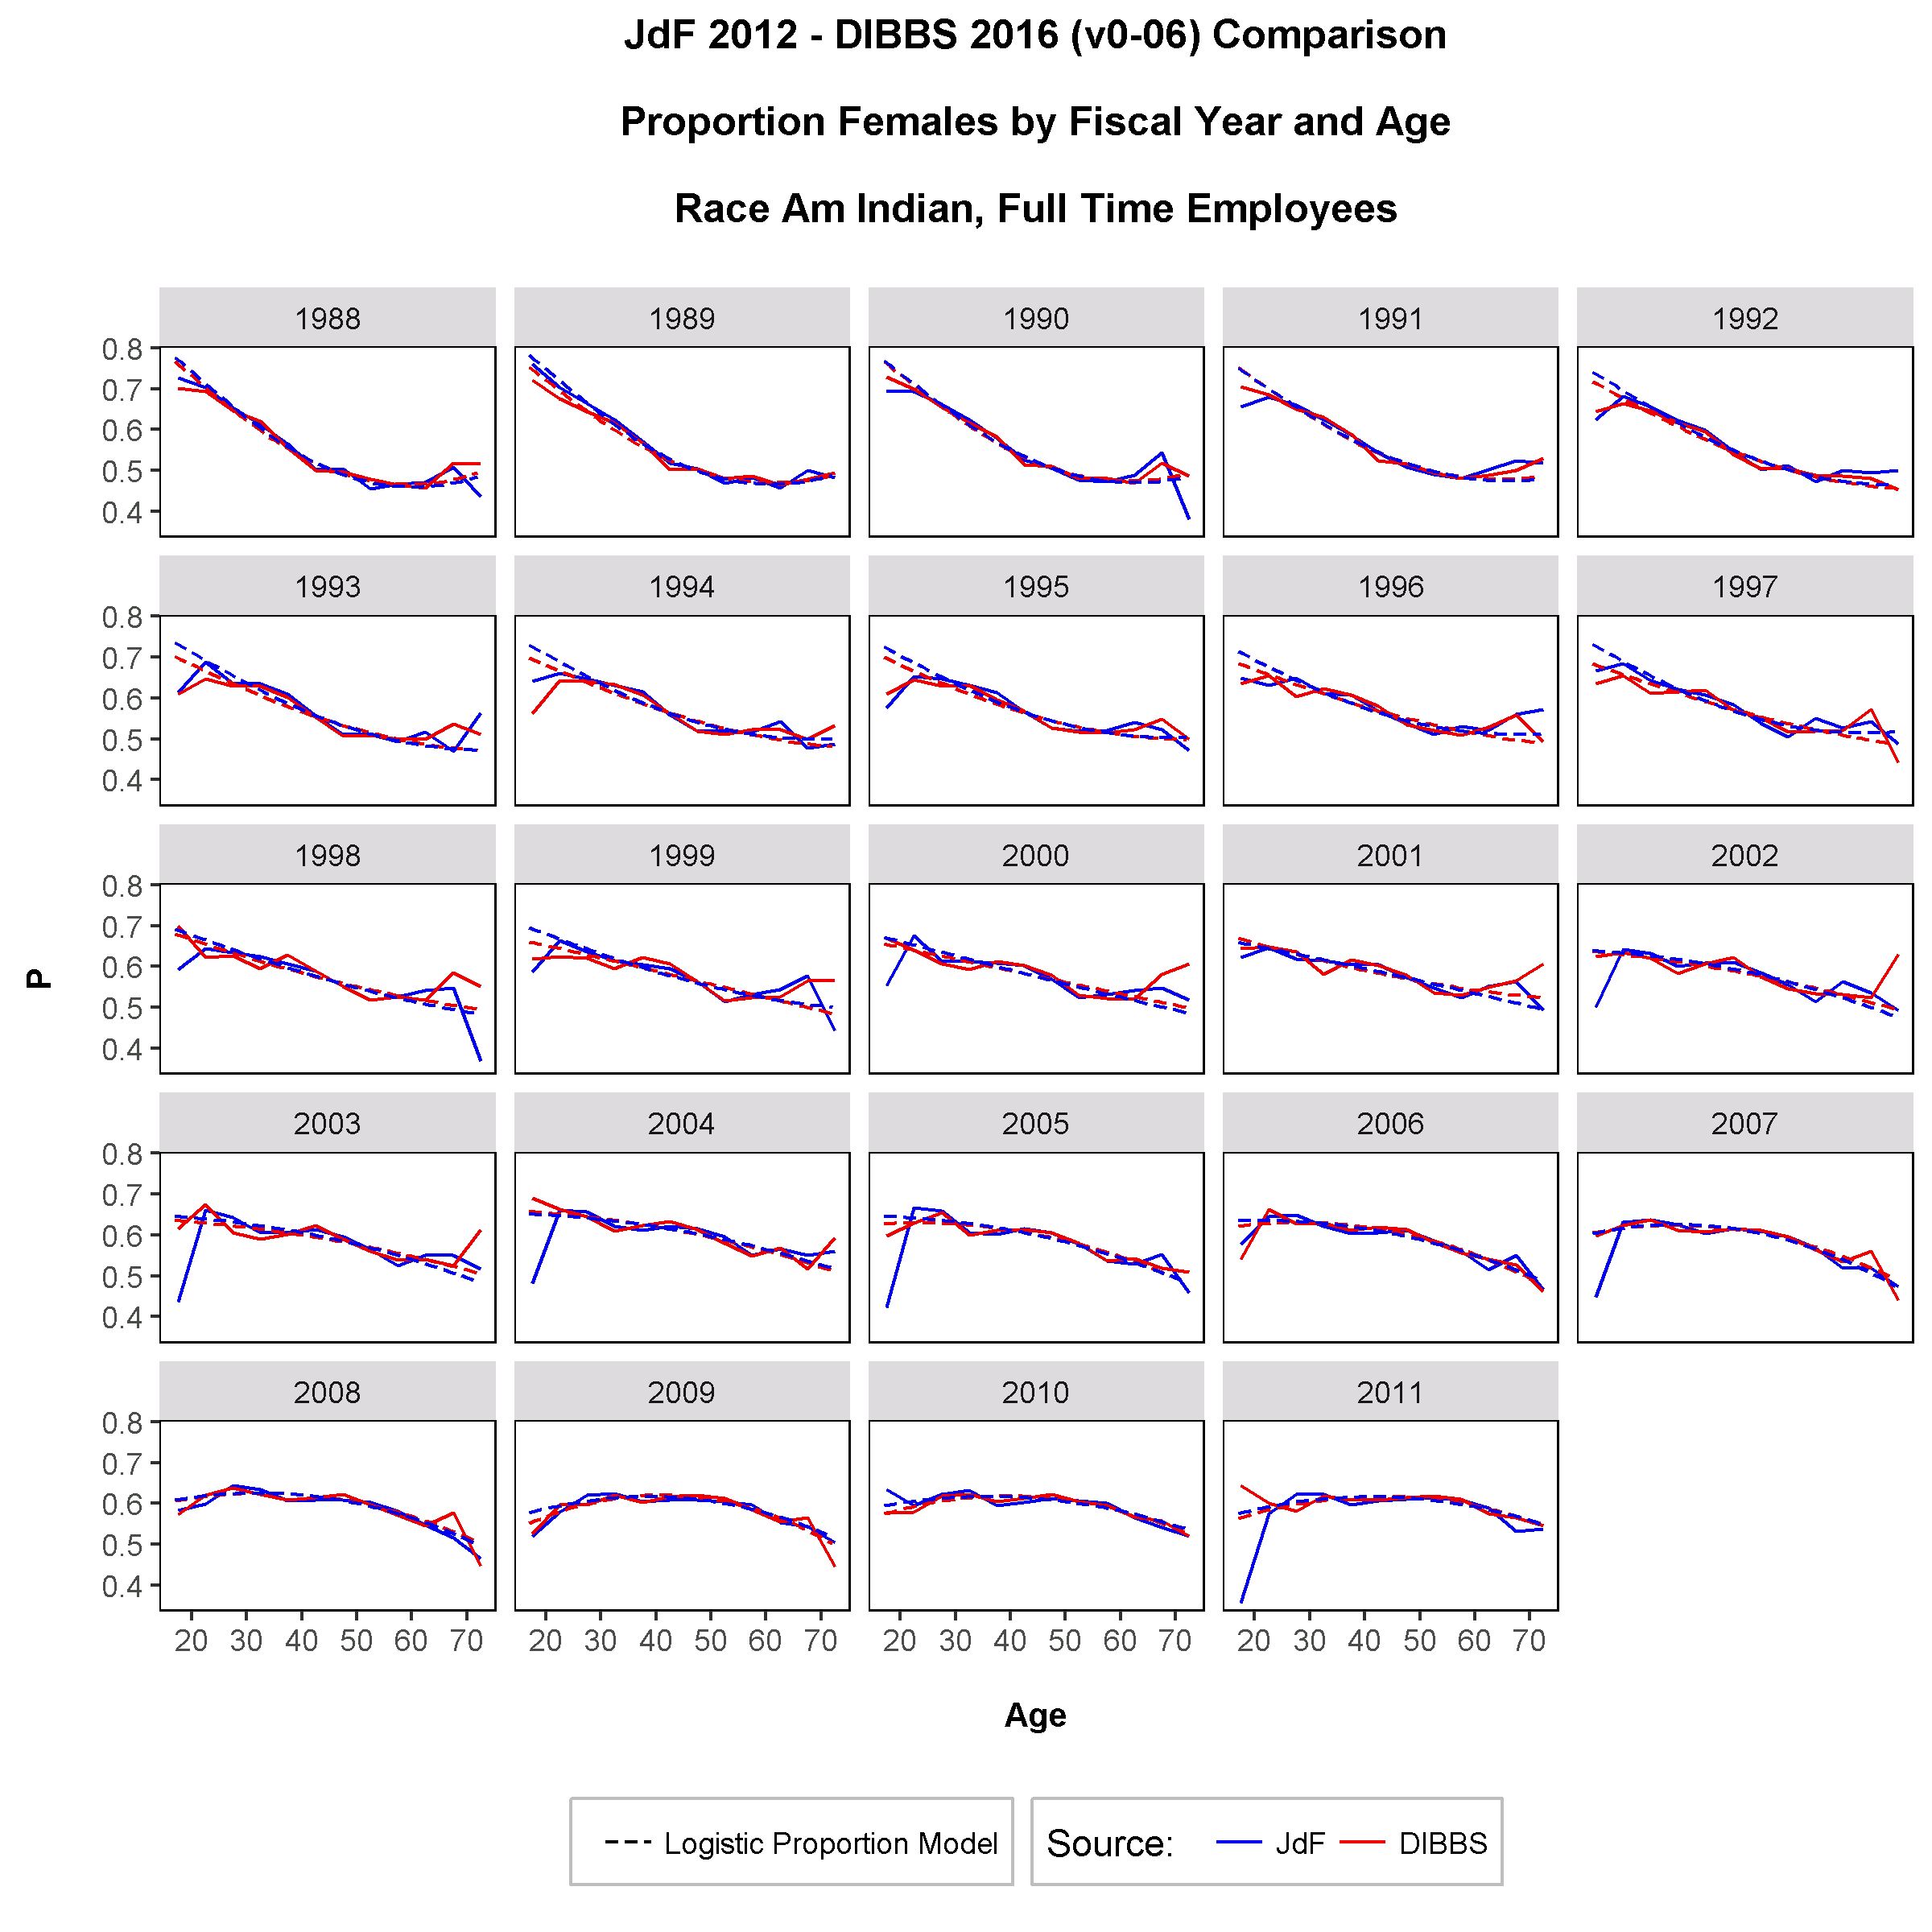
\includegraphics[width=6.5in, trim={0 0 0 1in}, clip]{GenderProportionLogisticModelFYRaceAgeAv0-06.png}
    \caption{Proportion female observations by education and year.  Race Native American.  Fitted lines are logistic regression estimates.}
    \label{figure:GenderProportionLogisticModelFYRaceAgeA}
\end{figure}

\clearpage

\begin{figure}[h]
    \centering
    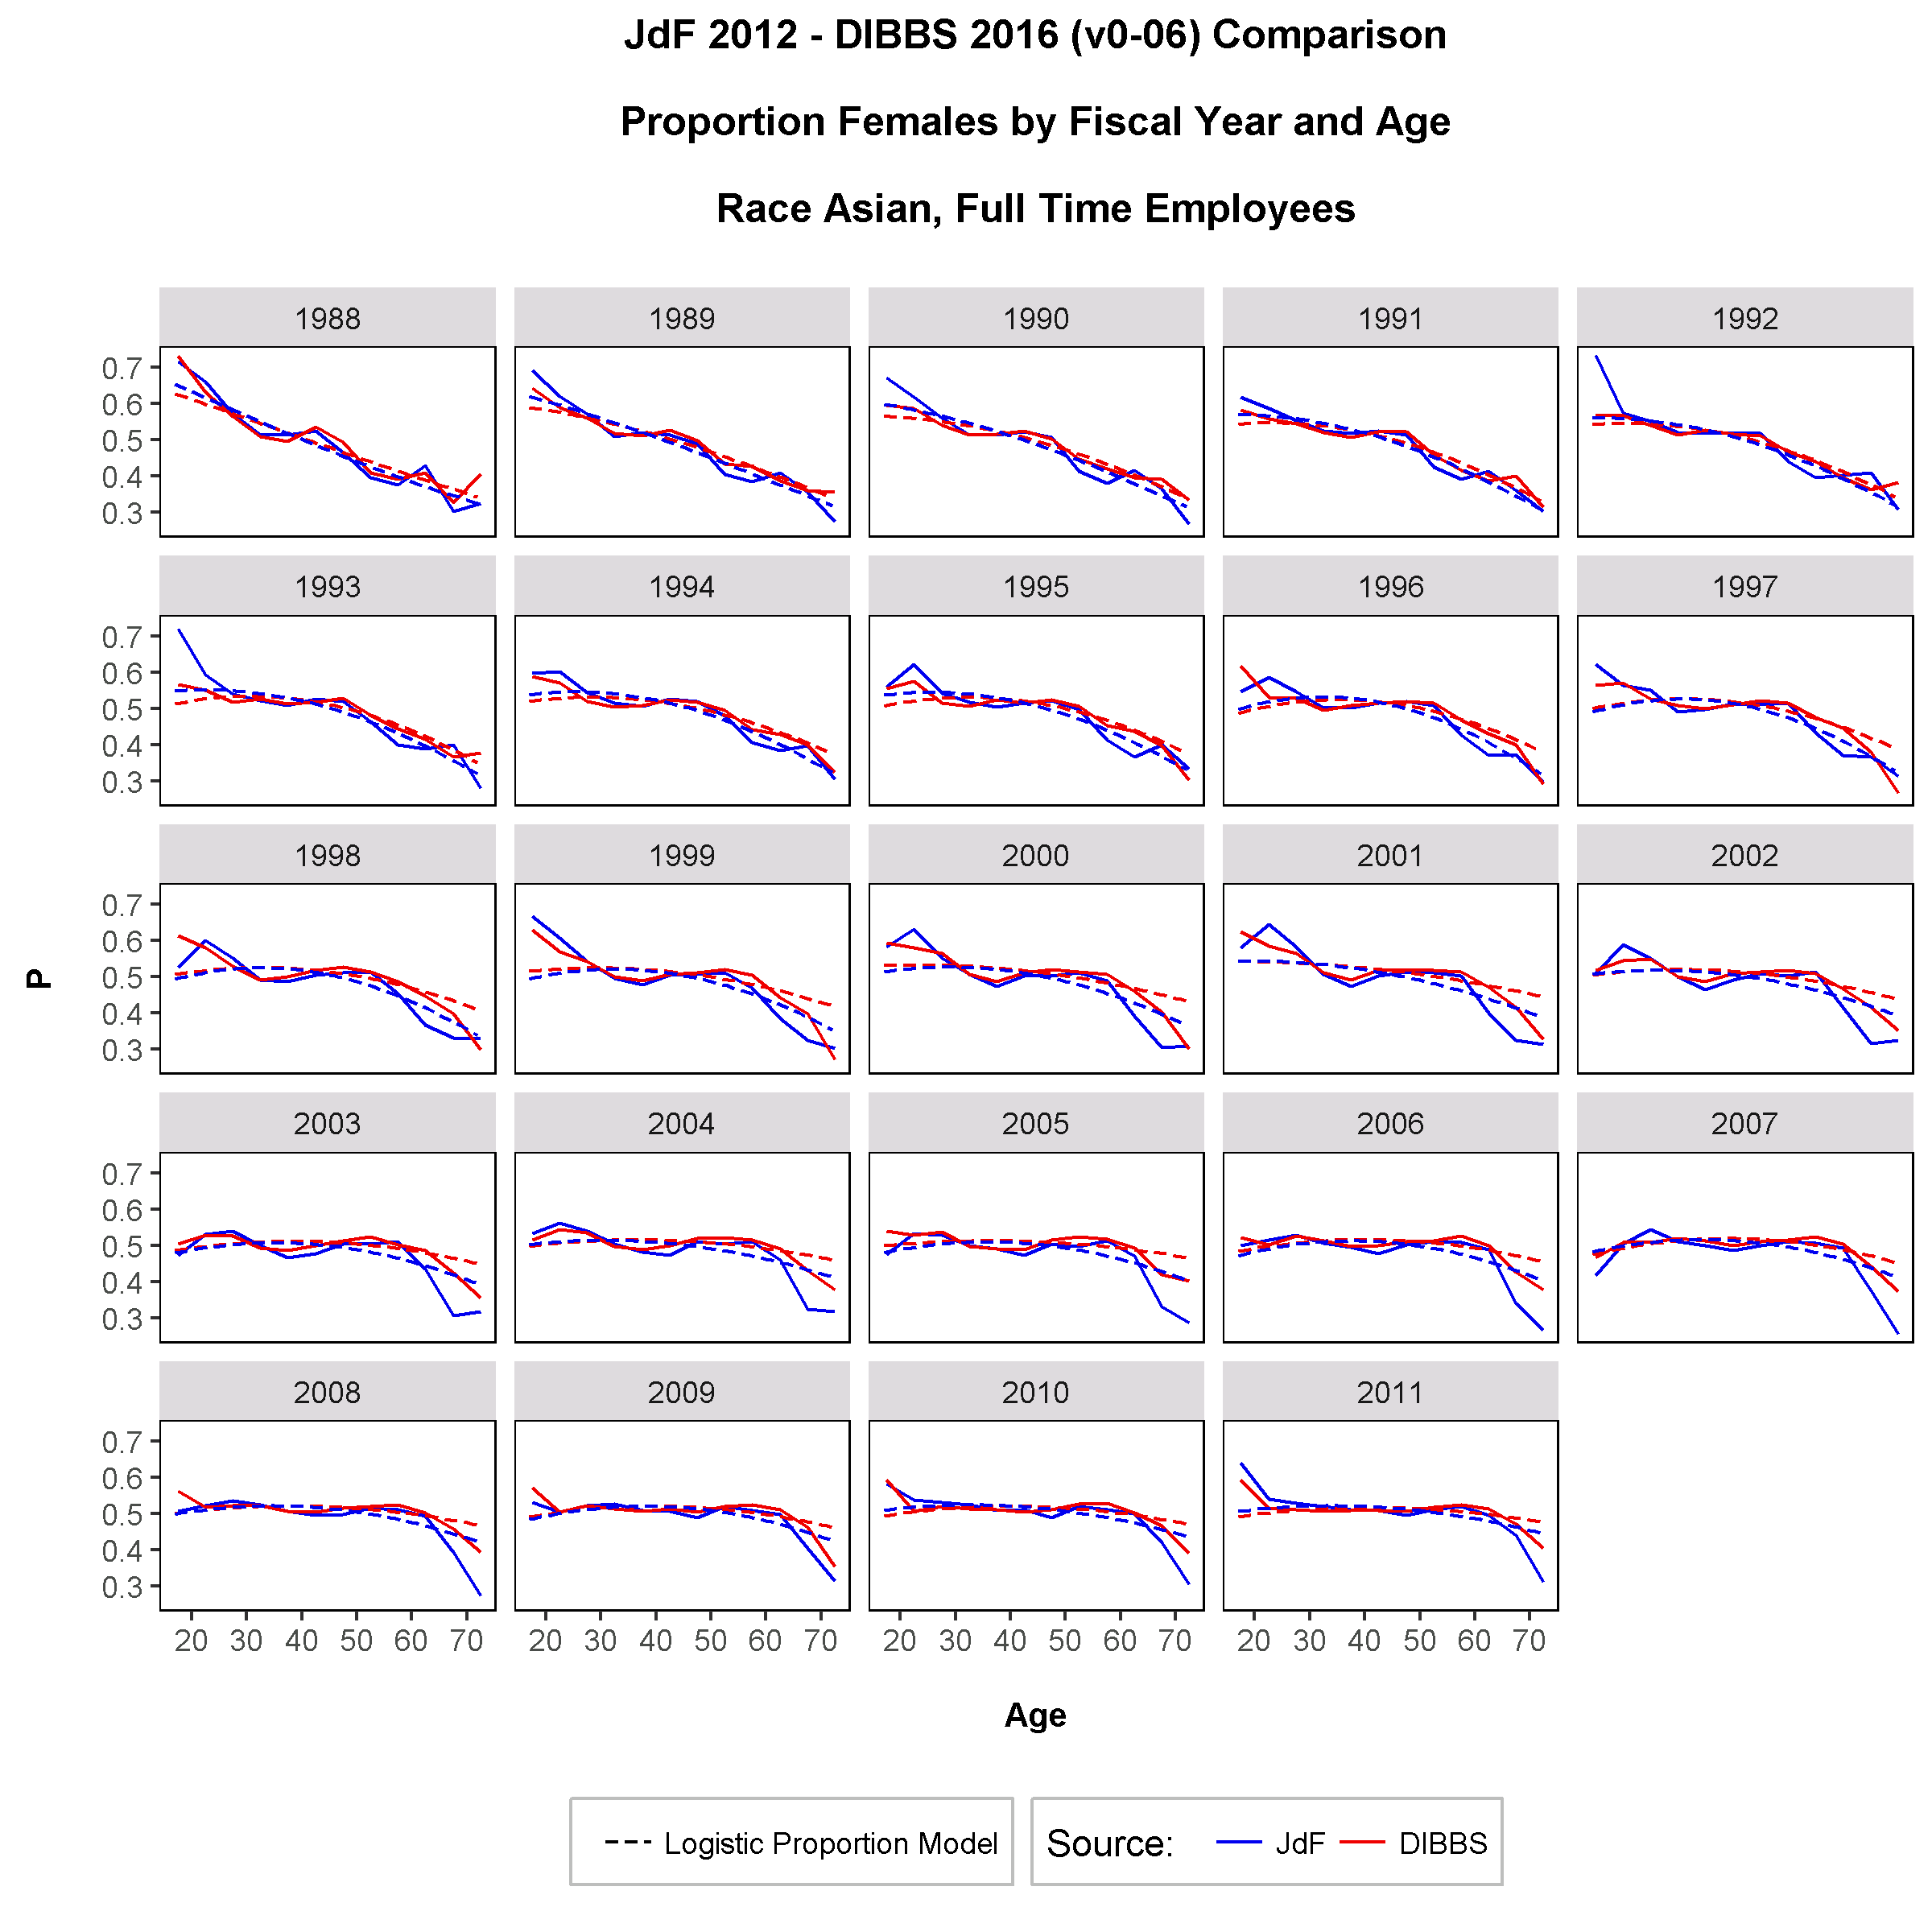
\includegraphics[width=6.5in, trim={0 0 0 1in}, clip]{GenderProportionLogisticModelFYRaceAgeBv0-06.png}
    \caption{Proportion female observations by education and year.  Race Asian.  Fitted lines are logistic regression estimates.}
    \label{figure:GenderProportionLogisticModelFYRaceAgeB}
\end{figure}

\clearpage

\begin{figure}[h]
    \centering
    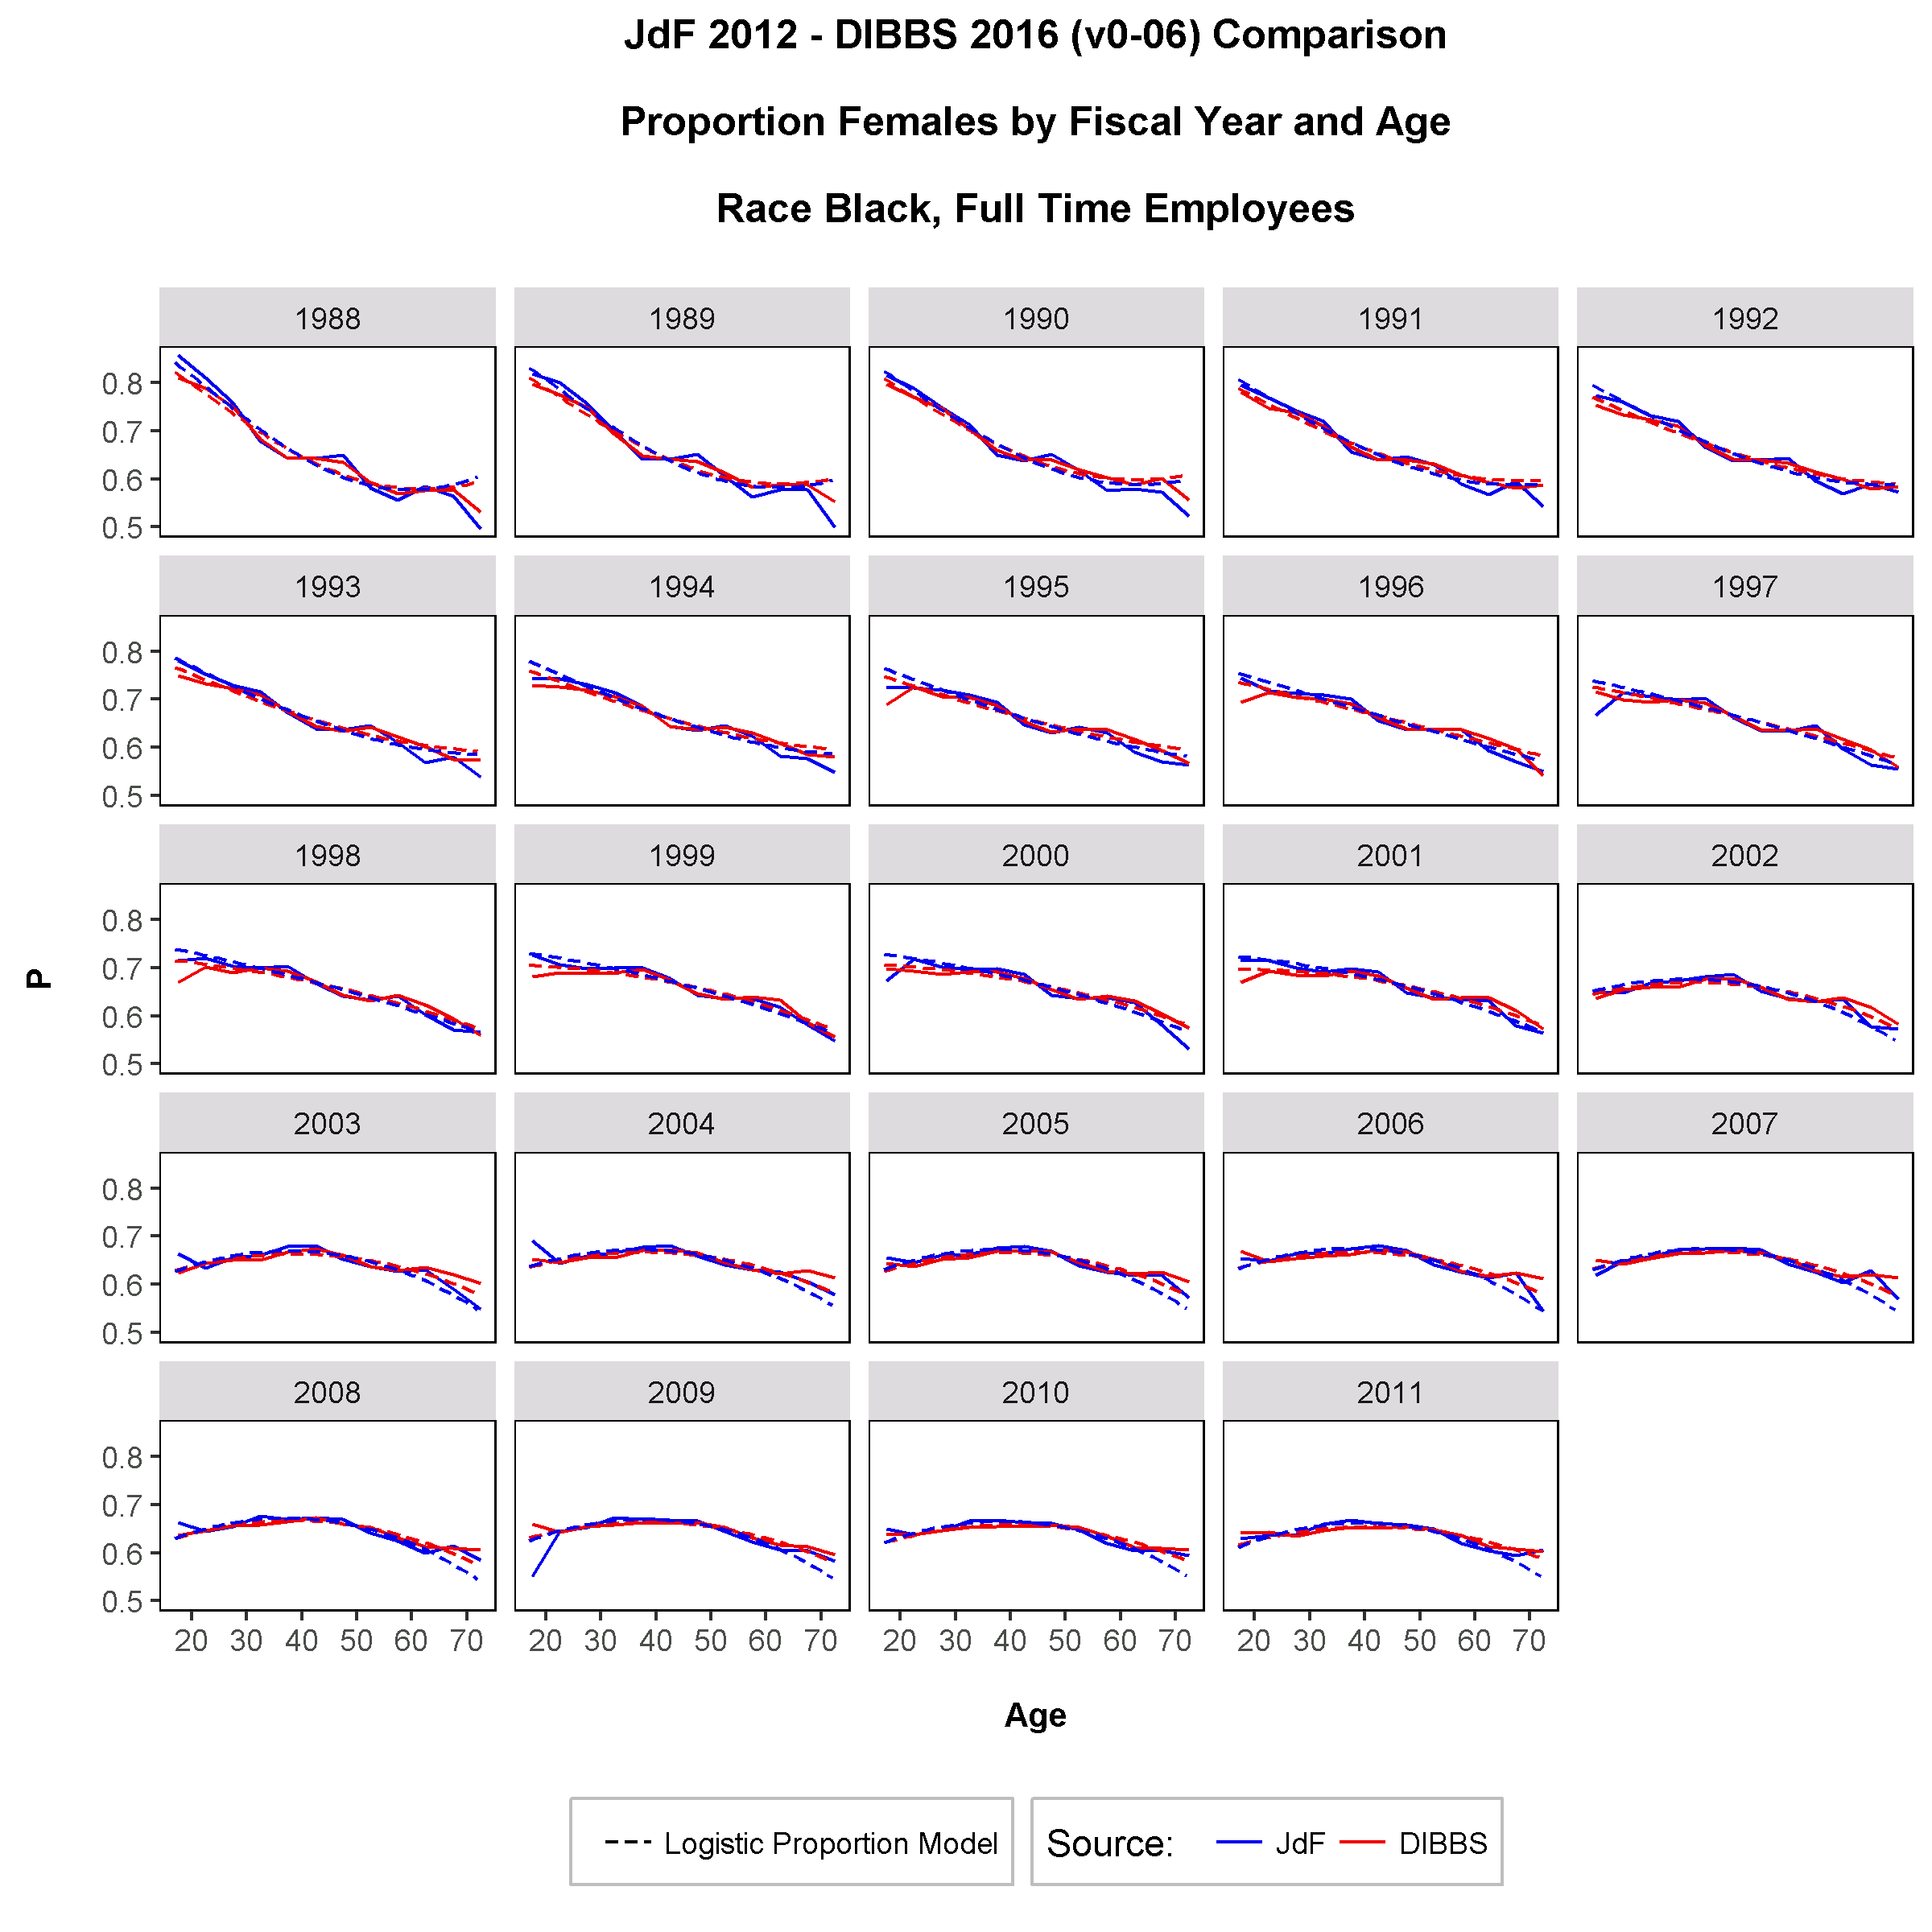
\includegraphics[width=6.5in, trim={0 0 0 1in}, clip]{GenderProportionLogisticModelFYRaceAgeCv0-06.png}
    \caption{Proportion female observations by education and year.  Race black.  Fitted lines are logistic regression estimates.}
    \label{figure:GenderProportionLogisticModelFYRaceAgeC}
\end{figure}

\clearpage

\begin{figure}[h]
    \centering
    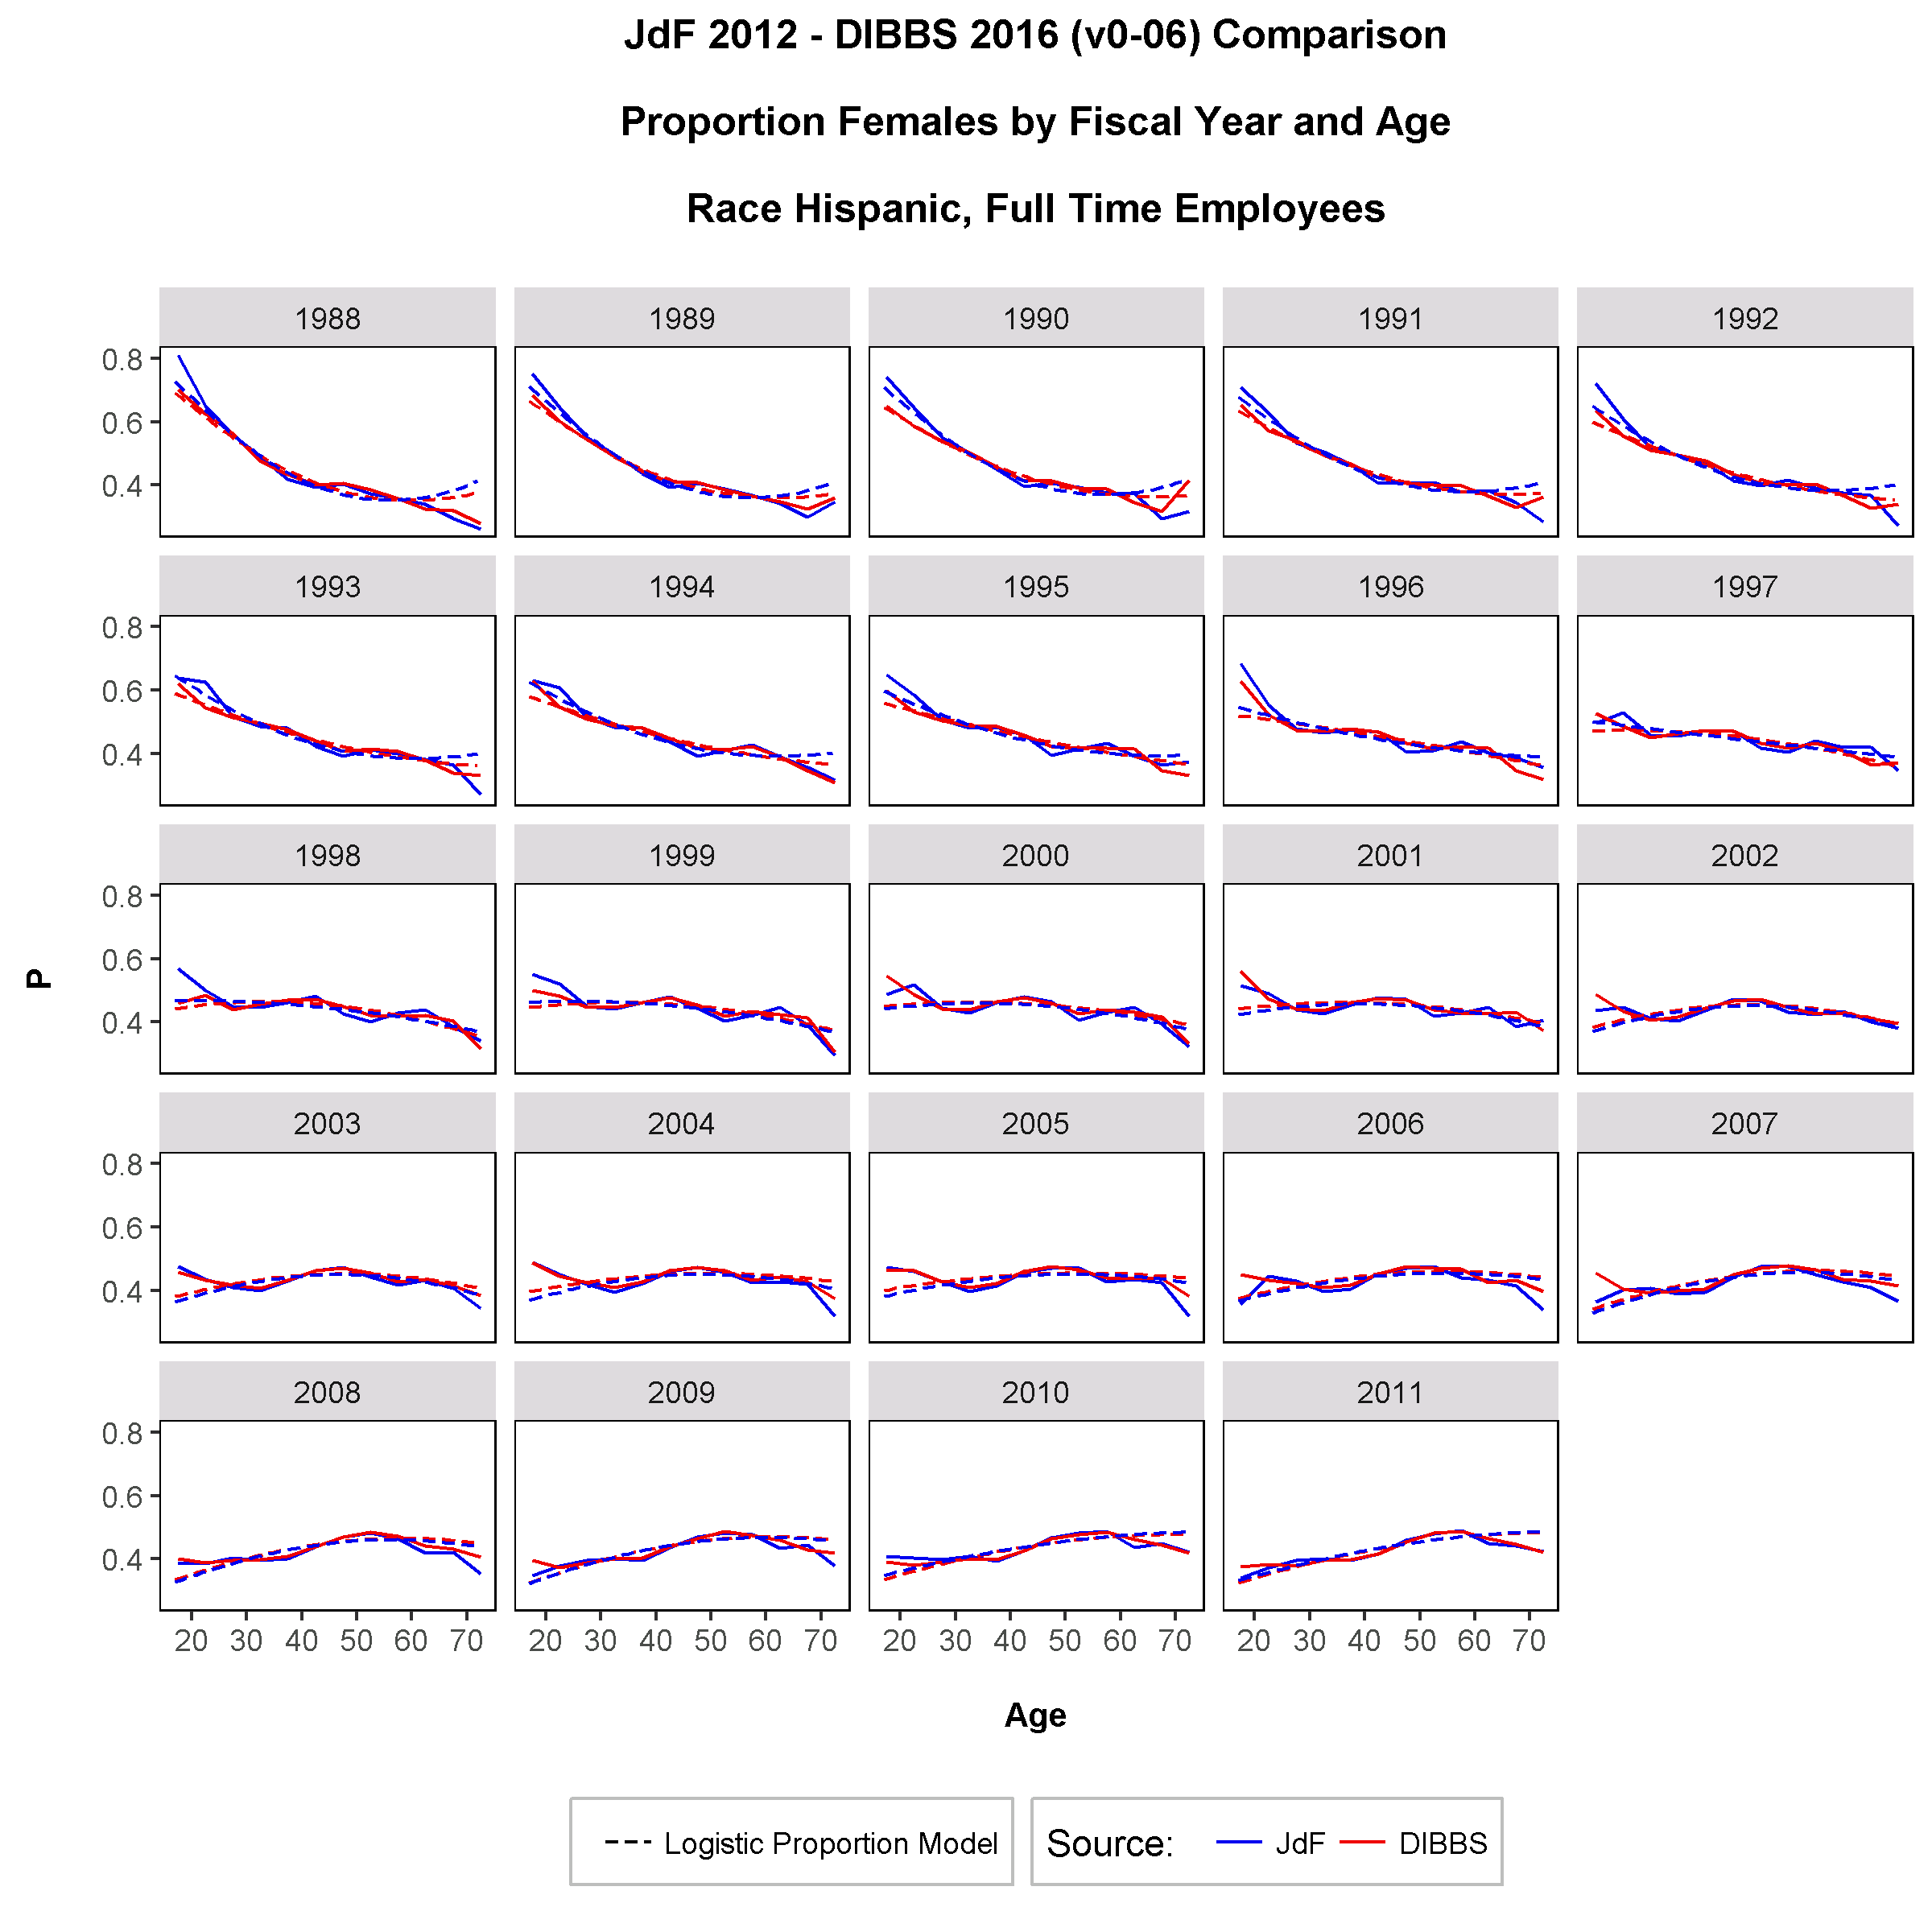
\includegraphics[width=6.5in, trim={0 0 0 1in}, clip]{GenderProportionLogisticModelFYRaceAgeDv0-06.png}
    \caption{Proportion female observations by education and year.  Race Hispanic.  Fitted lines are logistic regression estimates.}
    \label{figure:GenderProportionLogisticModelFYRaceAgeD}
\end{figure}

\clearpage

\begin{figure}[h]
\centering
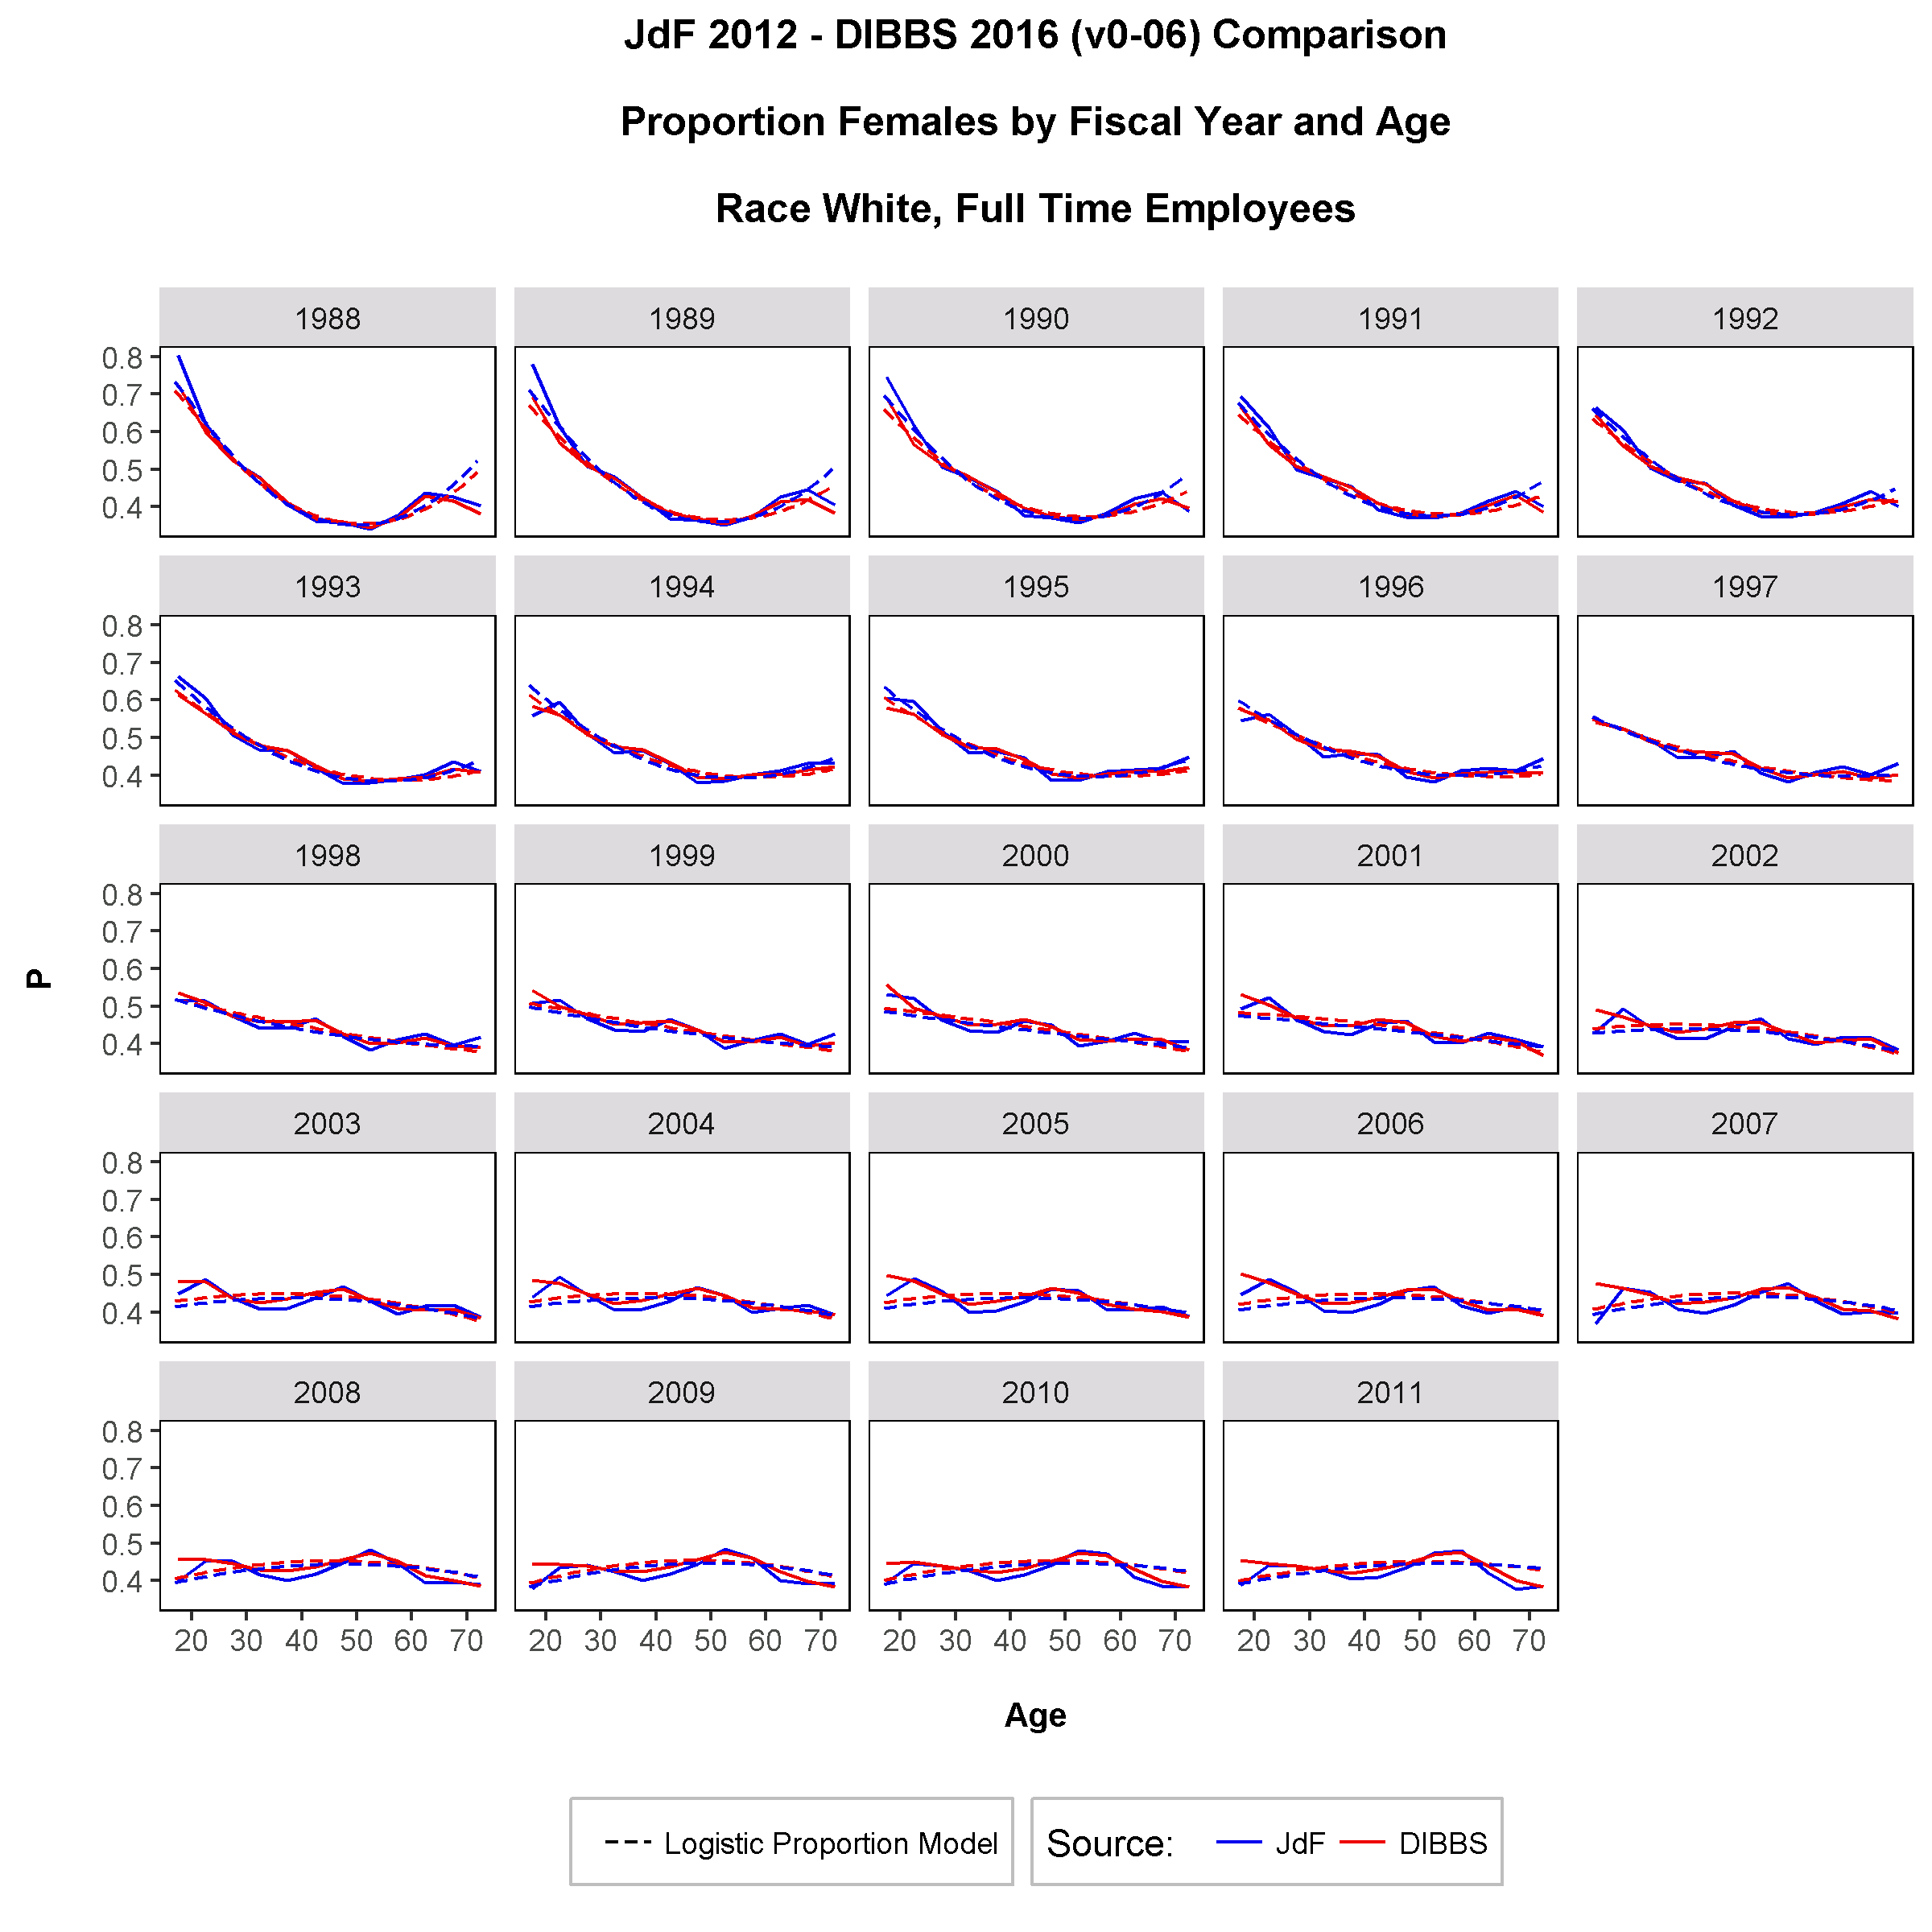
\includegraphics[width=6.5in, trim={0 0 0 1in}, clip]{GenderProportionLogisticModelFYRaceAgeEv0-06.png}
\caption{Proportion female observations by education and year.  Race white.  Fitted lines are logistic regression estimates.}
\label{figure:GenderProportionLogisticModelFYRaceAgeE}
\end{figure}

\clearpage





\end{spacing}


\newpage

\begingroup
\begin{spacing}{1.0}
    \raggedright
    \bibliography{DataUtilityBibliography}
\end{spacing}
\endgroup

\end{document}